\documentclass[twoside]{book}

% Packages required by doxygen
\usepackage{fixltx2e}
\usepackage{calc}
\usepackage{doxygen}
\usepackage[export]{adjustbox} % also loads graphicx
\usepackage{graphicx}
\usepackage[utf8]{inputenc}
\usepackage{makeidx}
\usepackage{multicol}
\usepackage{multirow}
\PassOptionsToPackage{warn}{textcomp}
\usepackage{textcomp}
\usepackage[nointegrals]{wasysym}
\usepackage[table]{xcolor}

% Font selection
\usepackage[T1]{fontenc}
\usepackage[scaled=.90]{helvet}
\usepackage{courier}
\usepackage{amssymb}
\usepackage{sectsty}
\renewcommand{\familydefault}{\sfdefault}
\allsectionsfont{%
  \fontseries{bc}\selectfont%
  \color{darkgray}%
}
\renewcommand{\DoxyLabelFont}{%
  \fontseries{bc}\selectfont%
  \color{darkgray}%
}
\newcommand{\+}{\discretionary{\mbox{\scriptsize$\hookleftarrow$}}{}{}}

% Page & text layout
\usepackage{geometry}
\geometry{%
  a4paper,%
  top=2.5cm,%
  bottom=2.5cm,%
  left=2.5cm,%
  right=2.5cm%
}
\tolerance=750
\hfuzz=15pt
\hbadness=750
\setlength{\emergencystretch}{15pt}
\setlength{\parindent}{0cm}
\setlength{\parskip}{3ex plus 2ex minus 2ex}
\makeatletter
\renewcommand{\paragraph}{%
  \@startsection{paragraph}{4}{0ex}{-1.0ex}{1.0ex}{%
    \normalfont\normalsize\bfseries\SS@parafont%
  }%
}
\renewcommand{\subparagraph}{%
  \@startsection{subparagraph}{5}{0ex}{-1.0ex}{1.0ex}{%
    \normalfont\normalsize\bfseries\SS@subparafont%
  }%
}
\makeatother

% Headers & footers
\usepackage{fancyhdr}
\pagestyle{fancyplain}
\fancyhead[LE]{\fancyplain{}{\bfseries\thepage}}
\fancyhead[CE]{\fancyplain{}{}}
\fancyhead[RE]{\fancyplain{}{\bfseries\leftmark}}
\fancyhead[LO]{\fancyplain{}{\bfseries\rightmark}}
\fancyhead[CO]{\fancyplain{}{}}
\fancyhead[RO]{\fancyplain{}{\bfseries\thepage}}
\fancyfoot[LE]{\fancyplain{}{}}
\fancyfoot[CE]{\fancyplain{}{}}
\fancyfoot[RE]{\fancyplain{}{\bfseries\scriptsize Generated by Doxygen }}
\fancyfoot[LO]{\fancyplain{}{\bfseries\scriptsize Generated by Doxygen }}
\fancyfoot[CO]{\fancyplain{}{}}
\fancyfoot[RO]{\fancyplain{}{}}
\renewcommand{\footrulewidth}{0.4pt}
\renewcommand{\chaptermark}[1]{%
  \markboth{#1}{}%
}
\renewcommand{\sectionmark}[1]{%
  \markright{\thesection\ #1}%
}

% Indices & bibliography
\usepackage{natbib}
\usepackage[titles]{tocloft}
\setcounter{tocdepth}{3}
\setcounter{secnumdepth}{5}
\makeindex

% Hyperlinks (required, but should be loaded last)
\usepackage{ifpdf}
\ifpdf
  \usepackage[pdftex,pagebackref=true]{hyperref}
\else
  \usepackage[ps2pdf,pagebackref=true]{hyperref}
\fi
\hypersetup{%
  colorlinks=true,%
  linkcolor=blue,%
  citecolor=blue,%
  unicode%
}

% Custom commands
\newcommand{\clearemptydoublepage}{%
  \newpage{\pagestyle{empty}\cleardoublepage}%
}

\usepackage{caption}
\captionsetup{labelsep=space,justification=centering,font={bf},singlelinecheck=off,skip=4pt,position=top}

%===== C O N T E N T S =====

\begin{document}

% Titlepage & ToC
\hypersetup{pageanchor=false,
             bookmarksnumbered=true,
             pdfencoding=unicode
            }
\pagenumbering{alph}
\begin{titlepage}
\vspace*{7cm}
\begin{center}%
{\Large Common-\/\+Architecture\+Dependent }\\
\vspace*{1cm}
{\large Generated by Doxygen 1.8.13}\\
\end{center}
\end{titlepage}
\clearemptydoublepage
\pagenumbering{roman}
\tableofcontents
\clearemptydoublepage
\pagenumbering{arabic}
\hypersetup{pageanchor=true}

%--- Begin generated contents ---
\chapter{Hierarchical Index}
\section{Class Hierarchy}
This inheritance list is sorted roughly, but not completely, alphabetically\+:\begin{DoxyCompactList}
\item \contentsline{section}{Arch}{\pageref{classArch}}{}
\item \contentsline{section}{Arch\+\_\+dep}{\pageref{classArch__dep}}{}
\begin{DoxyCompactList}
\item \contentsline{section}{A\+RM}{\pageref{classARM}}{}
\item \contentsline{section}{M\+I\+PS}{\pageref{classMIPS}}{}
\end{DoxyCompactList}
\item \contentsline{section}{D\+A\+A\+Instruction}{\pageref{classDAAInstruction}}{}
\begin{DoxyCompactList}
\item \contentsline{section}{Add}{\pageref{classAdd}}{}
\item \contentsline{section}{Addiu}{\pageref{classAddiu}}{}
\item \contentsline{section}{A\+R\+M\+\_\+\+B\+R\+A\+N\+CH}{\pageref{classARM__BRANCH}}{}
\item \contentsline{section}{A\+R\+M\+\_\+\+C\+O\+M\+M\+ON}{\pageref{classARM__COMMON}}{}
\begin{DoxyCompactList}
\item \contentsline{section}{A\+R\+M\+\_\+\+A\+DD}{\pageref{classARM__ADD}}{}
\item \contentsline{section}{A\+R\+M\+\_\+\+L\+O\+AD}{\pageref{classARM__LOAD}}{}
\item \contentsline{section}{A\+R\+M\+\_\+\+L\+O\+A\+D\+\_\+\+M\+U\+L\+T\+I\+P\+LE}{\pageref{classARM__LOAD__MULTIPLE}}{}
\item \contentsline{section}{A\+R\+M\+\_\+\+L\+O\+G\+I\+C\+AL}{\pageref{classARM__LOGICAL}}{}
\item \contentsline{section}{A\+R\+M\+\_\+\+M\+OV}{\pageref{classARM__MOV}}{}
\item \contentsline{section}{A\+R\+M\+\_\+\+M\+UL}{\pageref{classARM__MUL}}{}
\item \contentsline{section}{A\+R\+M\+\_\+\+R\+E\+V\+E\+R\+S\+E\+\_\+\+S\+UB}{\pageref{classARM__REVERSE__SUB}}{}
\item \contentsline{section}{A\+R\+M\+\_\+\+S\+H\+I\+FT}{\pageref{classARM__SHIFT}}{}
\item \contentsline{section}{A\+R\+M\+\_\+\+S\+T\+O\+RE}{\pageref{classARM__STORE}}{}
\item \contentsline{section}{A\+R\+M\+\_\+\+S\+U\+B\+T\+R\+A\+CT}{\pageref{classARM__SUBTRACT}}{}
\end{DoxyCompactList}
\item \contentsline{section}{A\+R\+M\+\_\+\+C\+O\+M\+P\+A\+RE}{\pageref{classARM__COMPARE}}{}
\item \contentsline{section}{A\+R\+M\+\_\+\+N\+OP}{\pageref{classARM__NOP}}{}
\item \contentsline{section}{A\+R\+M\+\_\+\+P\+OP}{\pageref{classARM__POP}}{}
\item \contentsline{section}{A\+R\+M\+\_\+\+P\+U\+SH}{\pageref{classARM__PUSH}}{}
\item \contentsline{section}{A\+R\+M\+\_\+\+S\+T\+O\+R\+E\+\_\+\+M\+U\+L\+T\+I\+P\+LE}{\pageref{classARM__STORE__MULTIPLE}}{}
\item \contentsline{section}{A\+R\+M\+\_\+\+T\+O\+D\+O\+\_\+\+L\+O\+IC}{\pageref{classARM__TODO__LOIC}}{}
\item \contentsline{section}{D\+Call}{\pageref{classDCall}}{}
\item \contentsline{section}{D\+Load}{\pageref{classDLoad}}{}
\item \contentsline{section}{D\+Store}{\pageref{classDStore}}{}
\item \contentsline{section}{Kill\+Op1}{\pageref{classKillOp1}}{}
\item \contentsline{section}{Kill\+Op2}{\pageref{classKillOp2}}{}
\item \contentsline{section}{Li}{\pageref{classLi}}{}
\item \contentsline{section}{Lui}{\pageref{classLui}}{}
\item \contentsline{section}{Move}{\pageref{classMove}}{}
\item \contentsline{section}{Nop}{\pageref{classNop}}{}
\item \contentsline{section}{Shift}{\pageref{classShift}}{}
\item \contentsline{section}{Subu}{\pageref{classSubu}}{}
\end{DoxyCompactList}
\item \contentsline{section}{Instruction\+Format}{\pageref{classInstructionFormat}}{}
\begin{DoxyCompactList}
\item \contentsline{section}{Addr}{\pageref{classAddr}}{}
\item \contentsline{section}{Empty}{\pageref{classEmpty}}{}
\item \contentsline{section}{Hex}{\pageref{classHex}}{}
\item \contentsline{section}{rd}{\pageref{classrd}}{}
\item \contentsline{section}{rd\+\_\+hex}{\pageref{classrd__hex}}{}
\item \contentsline{section}{rd\+\_\+int}{\pageref{classrd__int}}{}
\item \contentsline{section}{rd\+\_\+mem}{\pageref{classrd__mem}}{}
\item \contentsline{section}{rd\+\_\+mem\+\_\+int}{\pageref{classrd__mem__int}}{}
\item \contentsline{section}{rd\+\_\+mem\+\_\+rs}{\pageref{classrd__mem__rs}}{}
\item \contentsline{section}{rd\+\_\+mem\+\_\+rs\+\_\+shifter}{\pageref{classrd__mem__rs__shifter}}{}
\item \contentsline{section}{rd\+\_\+rd\+\_\+rs\+\_\+rs}{\pageref{classrd__rd__rs__rs}}{}
\item \contentsline{section}{rd\+\_\+rs}{\pageref{classrd__rs}}{}
\item \contentsline{section}{rd\+\_\+rs\+\_\+hex}{\pageref{classrd__rs__hex}}{}
\item \contentsline{section}{rd\+\_\+rs\+\_\+int}{\pageref{classrd__rs__int}}{}
\item \contentsline{section}{rd\+\_\+rs\+\_\+rs}{\pageref{classrd__rs__rs}}{}
\item \contentsline{section}{rd\+\_\+rs\+\_\+rs\+\_\+rs}{\pageref{classrd__rs__rs__rs}}{}
\item \contentsline{section}{rd\+\_\+rs\+\_\+rs\+\_\+shifter}{\pageref{classrd__rs__rs__shifter}}{}
\item \contentsline{section}{rd\+\_\+rs\+\_\+shifter}{\pageref{classrd__rs__shifter}}{}
\item \contentsline{section}{rdlist}{\pageref{classrdlist}}{}
\item \contentsline{section}{rds\+\_\+hex}{\pageref{classrds__hex}}{}
\item \contentsline{section}{rds\+\_\+int}{\pageref{classrds__int}}{}
\item \contentsline{section}{rds\+\_\+rdlist}{\pageref{classrds__rdlist}}{}
\item \contentsline{section}{rds\+\_\+rds\+\_\+rs\+\_\+rs}{\pageref{classrds__rds__rs__rs}}{}
\item \contentsline{section}{rds\+\_\+rslist}{\pageref{classrds__rslist}}{}
\item \contentsline{section}{rs}{\pageref{classrs}}{}
\item \contentsline{section}{rs\+\_\+addr}{\pageref{classrs__addr}}{}
\item \contentsline{section}{rs\+\_\+hex}{\pageref{classrs__hex}}{}
\item \contentsline{section}{rs\+\_\+int}{\pageref{classrs__int}}{}
\item \contentsline{section}{rs\+\_\+mem}{\pageref{classrs__mem}}{}
\item \contentsline{section}{rs\+\_\+mem\+\_\+int}{\pageref{classrs__mem__int}}{}
\item \contentsline{section}{rs\+\_\+mem\+\_\+rs}{\pageref{classrs__mem__rs}}{}
\item \contentsline{section}{rs\+\_\+mem\+\_\+rs\+\_\+shifter}{\pageref{classrs__mem__rs__shifter}}{}
\item \contentsline{section}{rs\+\_\+rd}{\pageref{classrs__rd}}{}
\item \contentsline{section}{rs\+\_\+rdlist}{\pageref{classrs__rdlist}}{}
\item \contentsline{section}{rs\+\_\+rs}{\pageref{classrs__rs}}{}
\item \contentsline{section}{rs\+\_\+rs\+\_\+addr}{\pageref{classrs__rs__addr}}{}
\item \contentsline{section}{rs\+\_\+rs\+\_\+shifter}{\pageref{classrs__rs__shifter}}{}
\item \contentsline{section}{rs\+\_\+rslist}{\pageref{classrs__rslist}}{}
\item \contentsline{section}{rs\+\_\+zero\+\_\+hex}{\pageref{classrs__zero__hex}}{}
\item \contentsline{section}{rslist}{\pageref{classrslist}}{}
\item \contentsline{section}{zero\+\_\+rs\+\_\+rs}{\pageref{classzero__rs__rs}}{}
\end{DoxyCompactList}
\item \contentsline{section}{Instruction\+Type}{\pageref{classInstructionType}}{}
\begin{DoxyCompactList}
\item \contentsline{section}{Basic}{\pageref{classBasic}}{}
\item \contentsline{section}{Call}{\pageref{classCall}}{}
\item \contentsline{section}{Conditional\+Jump}{\pageref{classConditionalJump}}{}
\item \contentsline{section}{Load}{\pageref{classLoad}}{}
\item \contentsline{section}{Predicated\+Basic}{\pageref{classPredicatedBasic}}{}
\item \contentsline{section}{Predicated\+Load}{\pageref{classPredicatedLoad}}{}
\item \contentsline{section}{Predicated\+Store}{\pageref{classPredicatedStore}}{}
\item \contentsline{section}{Return}{\pageref{classReturn}}{}
\item \contentsline{section}{Store}{\pageref{classStore}}{}
\item \contentsline{section}{Unconditional\+Jump}{\pageref{classUnconditionalJump}}{}
\item \contentsline{section}{Word}{\pageref{classWord}}{}
\end{DoxyCompactList}
\item \contentsline{section}{Objdump\+Function}{\pageref{classObjdumpFunction}}{}
\item \contentsline{section}{Objdump\+Instruction}{\pageref{classObjdumpInstruction}}{}
\item \contentsline{section}{Objdump\+Section}{\pageref{classObjdumpSection}}{}
\item \contentsline{section}{Objdump\+Symbol\+Table}{\pageref{classObjdumpSymbolTable}}{}
\item \contentsline{section}{Objdump\+Variable}{\pageref{classObjdumpVariable}}{}
\item \contentsline{section}{Objdump\+Word}{\pageref{classObjdumpWord}}{}
\end{DoxyCompactList}

\chapter{Class Index}
\section{Class List}
Here are the classes, structs, unions and interfaces with brief descriptions\+:\begin{DoxyCompactList}
\item\contentsline{section}{\hyperlink{classInstructionARM}{Instruction\+A\+RM} }{\pageref{classInstructionARM}}{}
\item\contentsline{section}{\hyperlink{classLogger}{Logger} }{\pageref{classLogger}}{}
\item\contentsline{section}{\hyperlink{classUtl}{Utl} }{\pageref{classUtl}}{}
\end{DoxyCompactList}

\chapter{File Index}
\section{File List}
Here is a list of all files with brief descriptions\+:\begin{DoxyCompactList}
\item\contentsline{section}{src/\hyperlink{AddressAttribute_8h}{Address\+Attribute.\+h} }{\pageref{AddressAttribute_8h}}{}
\item\contentsline{section}{src/\hyperlink{ARMWordsAttribute_8h}{A\+R\+M\+Words\+Attribute.\+h} }{\pageref{ARMWordsAttribute_8h}}{}
\item\contentsline{section}{src/\hyperlink{GlobalAttributes_8h}{Global\+Attributes.\+h} }{\pageref{GlobalAttributes_8h}}{}
\item\contentsline{section}{src/\hyperlink{LoopTree_8h}{Loop\+Tree.\+h} }{\pageref{LoopTree_8h}}{}
\item\contentsline{section}{src/\hyperlink{MetaInstructionAttribute_8h}{Meta\+Instruction\+Attribute.\+h} }{\pageref{MetaInstructionAttribute_8h}}{}
\item\contentsline{section}{src/\hyperlink{SymbolTableAttribute_8h}{Symbol\+Table\+Attribute.\+h} }{\pageref{SymbolTableAttribute_8h}}{}
\end{DoxyCompactList}

\chapter{Class Documentation}
\hypertarget{classAdd}{}\section{Add Class Reference}
\label{classAdd}\index{Add@{Add}}


{\ttfamily \#include $<$D\+A\+A\+Instruction\+\_\+\+M\+I\+P\+S.\+h$>$}

Inheritance diagram for Add\+:\begin{figure}[H]
\begin{center}
\leavevmode
\includegraphics[height=2.000000cm]{classAdd}
\end{center}
\end{figure}
\subsection*{Public Member Functions}
\begin{DoxyCompactItemize}
\item 
void \hyperlink{classAdd_a6048e7447a91cb9edd65eb94184f9494}{simulate} (vector$<$ string $>$ \&, vector$<$ bool $>$ \&, \hyperlink{DAAInstruction_8h_a1b0e70ac1a04f06c8132055ed01f589f}{stack\+Type} \&vstack, \hyperlink{DAAInstruction_8h_ac5cb793e9dac3fa9693da78b7e29ab30}{stack\+Prec\+Type} \&v\+Stack\+Precision, const string \&)
\end{DoxyCompactItemize}
\subsection*{Additional Inherited Members}


\subsection{Detailed Description}


 \subsubsection*{Arithmetic and Logical Instructions }

\subsection{Member Function Documentation}
\mbox{\Hypertarget{classAdd_a6048e7447a91cb9edd65eb94184f9494}\label{classAdd_a6048e7447a91cb9edd65eb94184f9494}} 
\index{Add@{Add}!simulate@{simulate}}
\index{simulate@{simulate}!Add@{Add}}
\subsubsection{\texorpdfstring{simulate()}{simulate()}}
{\footnotesize\ttfamily void Add\+::simulate (\begin{DoxyParamCaption}\item[{vector$<$ string $>$ \&}]{regs,  }\item[{vector$<$ bool $>$ \&}]{precision,  }\item[{\hyperlink{DAAInstruction_8h_a1b0e70ac1a04f06c8132055ed01f589f}{stack\+Type} \&}]{vstack,  }\item[{\hyperlink{DAAInstruction_8h_ac5cb793e9dac3fa9693da78b7e29ab30}{stack\+Prec\+Type} \&}]{v\+Stack\+Precision,  }\item[{const string \&}]{asm\+Instr }\end{DoxyParamCaption})\hspace{0.3cm}{\ttfamily [virtual]}}

An instruction must implement a method simulate to compute the state of registers after its execution.

regs contains the contents of the machine registers before the simulation of the instruction. In case some computation can be done on register contents, simulate keeps the computation in textual format (ex\+: \char`\"{}sp+4\char`\"{}). String \char`\"{}$\ast$\char`\"{} denote that nothing is known about the register (and then the precision for the given register is set to false).

asm\+Instr (input) contains the textual representation of the instruction

precision contains information on registers whose contents is known precisely.

There are situations where the contents of a register is not set to \char`\"{}$\ast$\char`\"{} and its precision is set to false (see for instance, instructions of category add, used to compute offsets in arrays)

Rq\+: regs and precision are modified by the simulate function 

Implements \hyperlink{classDAAInstruction_a61d0b9bece1e0ead89a46c0197276324}{D\+A\+A\+Instruction}.



The documentation for this class was generated from the following file\+:\begin{DoxyCompactItemize}
\item 
src/\hyperlink{DAAInstruction__MIPS_8h}{D\+A\+A\+Instruction\+\_\+\+M\+I\+P\+S.\+h}\end{DoxyCompactItemize}

\hypertarget{classAddiu}{}\section{Addiu Class Reference}
\label{classAddiu}\index{Addiu@{Addiu}}


{\ttfamily \#include $<$D\+A\+A\+Instruction\+\_\+\+M\+I\+P\+S.\+h$>$}

Inheritance diagram for Addiu\+:\begin{figure}[H]
\begin{center}
\leavevmode
\includegraphics[height=2.000000cm]{classAddiu}
\end{center}
\end{figure}
\subsection*{Public Member Functions}
\begin{DoxyCompactItemize}
\item 
void \hyperlink{classAddiu_aeb693e0251545bee996d120e0c8b245d}{simulate} (vector$<$ string $>$ \&, vector$<$ bool $>$ \&, \hyperlink{DAAInstruction_8h_a1b0e70ac1a04f06c8132055ed01f589f}{stack\+Type} \&vstack, \hyperlink{DAAInstruction_8h_ac5cb793e9dac3fa9693da78b7e29ab30}{stack\+Prec\+Type} \&v\+Stack\+Precision, const string \&)
\end{DoxyCompactItemize}
\subsection*{Additional Inherited Members}


\subsection{Member Function Documentation}
\mbox{\Hypertarget{classAddiu_aeb693e0251545bee996d120e0c8b245d}\label{classAddiu_aeb693e0251545bee996d120e0c8b245d}} 
\index{Addiu@{Addiu}!simulate@{simulate}}
\index{simulate@{simulate}!Addiu@{Addiu}}
\subsubsection{\texorpdfstring{simulate()}{simulate()}}
{\footnotesize\ttfamily void Addiu\+::simulate (\begin{DoxyParamCaption}\item[{vector$<$ string $>$ \&}]{regs,  }\item[{vector$<$ bool $>$ \&}]{precision,  }\item[{\hyperlink{DAAInstruction_8h_a1b0e70ac1a04f06c8132055ed01f589f}{stack\+Type} \&}]{vstack,  }\item[{\hyperlink{DAAInstruction_8h_ac5cb793e9dac3fa9693da78b7e29ab30}{stack\+Prec\+Type} \&}]{v\+Stack\+Precision,  }\item[{const string \&}]{asm\+Instr }\end{DoxyParamCaption})\hspace{0.3cm}{\ttfamily [virtual]}}

An instruction must implement a method simulate to compute the state of registers after its execution.

regs contains the contents of the machine registers before the simulation of the instruction. In case some computation can be done on register contents, simulate keeps the computation in textual format (ex\+: \char`\"{}sp+4\char`\"{}). String \char`\"{}$\ast$\char`\"{} denote that nothing is known about the register (and then the precision for the given register is set to false).

asm\+Instr (input) contains the textual representation of the instruction

precision contains information on registers whose contents is known precisely.

There are situations where the contents of a register is not set to \char`\"{}$\ast$\char`\"{} and its precision is set to false (see for instance, instructions of category add, used to compute offsets in arrays)

Rq\+: regs and precision are modified by the simulate function 

Implements \hyperlink{classDAAInstruction_a61d0b9bece1e0ead89a46c0197276324}{D\+A\+A\+Instruction}.



The documentation for this class was generated from the following file\+:\begin{DoxyCompactItemize}
\item 
src/\hyperlink{DAAInstruction__MIPS_8h}{D\+A\+A\+Instruction\+\_\+\+M\+I\+P\+S.\+h}\end{DoxyCompactItemize}

\hypertarget{classAddr}{}\section{Addr Class Reference}
\label{classAddr}\index{Addr@{Addr}}


{\ttfamily \#include $<$Instruction\+Format.\+h$>$}

Inheritance diagram for Addr\+:\begin{figure}[H]
\begin{center}
\leavevmode
\includegraphics[height=2.000000cm]{classAddr}
\end{center}
\end{figure}
\subsection*{Public Member Functions}
\begin{DoxyCompactItemize}
\item 
bool \hyperlink{classAddr_aff6fd4bf7c93990b1427843fff9069ed}{is\+Format} (const vector$<$ string $>$ \&operands)
\item 
vector$<$ string $>$ \hyperlink{classAddr_a0ed20cdb01d8b11b023fa3b5e54bab29}{get\+Resource\+Inputs} (const vector$<$ string $>$ \&operands)
\item 
vector$<$ string $>$ \hyperlink{classAddr_aa42b861112df7333d93b3dd242e6621b}{get\+Resource\+Outputs} (const vector$<$ string $>$ \&operands)
\end{DoxyCompactItemize}


\subsection{Member Function Documentation}
\mbox{\Hypertarget{classAddr_a0ed20cdb01d8b11b023fa3b5e54bab29}\label{classAddr_a0ed20cdb01d8b11b023fa3b5e54bab29}} 
\index{Addr@{Addr}!get\+Resource\+Inputs@{get\+Resource\+Inputs}}
\index{get\+Resource\+Inputs@{get\+Resource\+Inputs}!Addr@{Addr}}
\subsubsection{\texorpdfstring{get\+Resource\+Inputs()}{getResourceInputs()}}
{\footnotesize\ttfamily vector$<$string$>$ Addr\+::get\+Resource\+Inputs (\begin{DoxyParamCaption}\item[{const vector$<$ string $>$ \&}]{operands }\end{DoxyParamCaption})\hspace{0.3cm}{\ttfamily [virtual]}}

Returns the input resources 

Implements \hyperlink{classInstructionFormat_a09775d3a3c22f40a0f44504664e586e4}{Instruction\+Format}.

\mbox{\Hypertarget{classAddr_aa42b861112df7333d93b3dd242e6621b}\label{classAddr_aa42b861112df7333d93b3dd242e6621b}} 
\index{Addr@{Addr}!get\+Resource\+Outputs@{get\+Resource\+Outputs}}
\index{get\+Resource\+Outputs@{get\+Resource\+Outputs}!Addr@{Addr}}
\subsubsection{\texorpdfstring{get\+Resource\+Outputs()}{getResourceOutputs()}}
{\footnotesize\ttfamily vector$<$string$>$ Addr\+::get\+Resource\+Outputs (\begin{DoxyParamCaption}\item[{const vector$<$ string $>$ \&}]{operands }\end{DoxyParamCaption})\hspace{0.3cm}{\ttfamily [virtual]}}

Returns the output resources 

Implements \hyperlink{classInstructionFormat_a95cd28ffb1bde59b67f676880ab10536}{Instruction\+Format}.

\mbox{\Hypertarget{classAddr_aff6fd4bf7c93990b1427843fff9069ed}\label{classAddr_aff6fd4bf7c93990b1427843fff9069ed}} 
\index{Addr@{Addr}!is\+Format@{is\+Format}}
\index{is\+Format@{is\+Format}!Addr@{Addr}}
\subsubsection{\texorpdfstring{is\+Format()}{isFormat()}}
{\footnotesize\ttfamily bool Addr\+::is\+Format (\begin{DoxyParamCaption}\item[{const vector$<$ string $>$ \&}]{operands }\end{DoxyParamCaption})\hspace{0.3cm}{\ttfamily [virtual]}}

Returns true if operands match the format 

Implements \hyperlink{classInstructionFormat_a9fdcf94dcd7d9a55ba86e7a63f04d1fe}{Instruction\+Format}.



The documentation for this class was generated from the following file\+:\begin{DoxyCompactItemize}
\item 
src/\hyperlink{InstructionFormat_8h}{Instruction\+Format.\+h}\end{DoxyCompactItemize}

\hypertarget{classArch}{}\section{Arch Class Reference}
\label{classArch}\index{Arch@{Arch}}


{\ttfamily \#include $<$arch.\+h$>$}

\subsection*{Static Public Member Functions}
\begin{DoxyCompactItemize}
\item 
static void \hyperlink{classArch_a6e55f92618422dfae2ecca4a8b760749}{init} (const string \&arch, const bool is\+\_\+big\+\_\+endian)
\item 
static void \hyperlink{classArch_a82f5b240caba345011c64b87f69d3573}{kill} ()
\item 
static \hyperlink{classArch__dep}{Arch\+\_\+dep} $\ast$ \hyperlink{classArch_a384595c0b0c27547c494ce68ea30390d}{get\+Instance} ()
\item 
static bool \hyperlink{classArch_a48a567260b0b9213386f2d1826f8e21c}{is\+Call} (const \hyperlink{classObjdumpInstruction}{Objdump\+Instruction} \&instr)
\item 
static bool \hyperlink{classArch_ad7b08b24c7d2e633ccb773fe9bd22489}{is\+Return} (const \hyperlink{classObjdumpInstruction}{Objdump\+Instruction} \&instr)
\item 
static bool \hyperlink{classArch_a852783c61c3b3c8d5b1025938fb59694}{is\+Unconditional\+Jump} (const \hyperlink{classObjdumpInstruction}{Objdump\+Instruction} \&instr)
\item 
static bool \hyperlink{classArch_a4384bfd7646ca7e0c945d6fb3b36db6f}{is\+Conditional\+Jump} (const \hyperlink{classObjdumpInstruction}{Objdump\+Instruction} \&instr)
\item 
static bool \hyperlink{classArch_a7c6ebd1702f075660199527678bd8612}{is\+Function} (const string \&line)
\item 
static bool \hyperlink{classArch_abcdc8f59823fa08c8dc1e06f67591e60}{is\+Instruction} (const string \&line)
\item 
static \hyperlink{classObjdumpFunction}{Objdump\+Function} \hyperlink{classArch_a086a563f23dcbab36b7238d131201471}{parse\+Function} (const string \&line)
\item 
static \hyperlink{classObjdumpInstruction}{Objdump\+Instruction} \hyperlink{classArch_a15814eafabeb6142fa46098767617d83}{parse\+Instruction} (const string \&line)
\item 
static t\+\_\+address \hyperlink{classArch_a14e634f478d8e7f6b76680184ffdddaf}{get\+Jump\+Destination} (const \hyperlink{classObjdumpInstruction}{Objdump\+Instruction} \&instr)
\item 
static int \hyperlink{classArch_a2cfdbdf8fe0435d65ce6549c4683fd0c}{get\+N\+B\+Instr\+In\+Delay\+Slot} ()
\item 
static int \hyperlink{classArch_af990ba7bfa96246fe0eda6248b5a9608}{get\+Instruction\+Size} ()
\item 
static bool \hyperlink{classArch_ad5c5d6cd8d1a555d0949baadfb83f59a}{is\+Mem\+Pattern} (const string \&operand)
\item 
static \hyperlink{classInstructionType}{Instruction\+Type} $\ast$ \hyperlink{classArch_adc29a91e6fd178a49f2bde6dcc441784}{get\+Instruction\+Type\+From\+Mnemonic} (const string \&mnemonic)
\item 
static \hyperlink{classInstructionType}{Instruction\+Type} $\ast$ \hyperlink{classArch_a25ad6eb3a759792bcb793b61cf629da0}{get\+Instruction\+Type\+From\+Asm} (const string \&instr)
\item 
static int \hyperlink{classArch_ad443b9fd33ae50f27aec5263ba980c47}{get\+Register\+Number} (const string \&reg\+\_\+name)
\item 
static bool \hyperlink{classArch_a23765c24091362fb1e974fba027cdfb1}{is\+Register\+Name} (const string \&reg\+\_\+name)
\item 
static bool \hyperlink{classArch_a5bd70d25a0dcb59d10cdb717c43842f2}{is\+Zero\+Register} (const string \&str)
\item 
static bool \hyperlink{classArch_ab872a6e1e060fce6dbd631ade563a482}{is\+Dec\+Number} (const string \&str)
\item 
static bool \hyperlink{classArch_a98b7249989defd4bdc9cd672592a0262}{is\+Hex\+Number} (const string \&str)
\item 
static bool \hyperlink{classArch_ada2832978d79268be376c443b65b37ed}{is\+Addr} (const string \&str)
\item 
static bool \hyperlink{classArch_a93077d5c7b72a0db0bea3bda59ca50c7}{is\+Load} (const string \&instr)
\item 
static bool \hyperlink{classArch_ab892d0c0ee92b3f04d371e84af1c44da}{is\+Store} (const string \&instr)
\item 
static int \hyperlink{classArch_ad07f05d2dfa30d60ae8a32642b029d10}{get\+Size\+Of\+Memory\+Access} (const string \&instr)
\item 
static bool \hyperlink{classArch_a580b03c8503aa94ed44905e2f525c6fb}{is\+Big\+Endian} ()
\item 
static vector$<$ string $>$ \hyperlink{classArch_a02fb24c4a3666859e5d503b370f980ec}{split\+Instruction} (const string \&instr)
\item 
static \hyperlink{classDAAInstruction}{D\+A\+A\+Instruction} $\ast$ \hyperlink{classArch_a056d89310ba797b493afff641bcc15c6}{get\+D\+A\+A\+Instruction} (const string \&instr)
\item 
static int \hyperlink{classArch_a4d1796b17b9dbaabed38ab10b8057013}{get\+Latency} (const string \&instr)
\item 
static vector$<$ string $>$ \hyperlink{classArch_ad43d2ee62f26a9fa2e193fa3a6cc8935}{extract\+Input\+Registers\+From\+Mem} (const string \&operand)
\item 
static vector$<$ string $>$ \hyperlink{classArch_a620da5dee3720e53e49e97ce6d7b3e0f}{extract\+Output\+Registers\+From\+Mem} (const string \&operand)
\item 
static vector$<$ string $>$ \hyperlink{classArch_a422c4ccd83e3652e7f11158272198397}{get\+Resource\+Functional\+Units} (const string \&instr)
\item 
static vector$<$ string $>$ \hyperlink{classArch_ac228ffb5a673b5250d0517a5bf6813b4}{get\+Resource\+Inputs} (const string \&instr)
\item 
static vector$<$ string $>$ \hyperlink{classArch_a368512825e8cdad354097faf60101ec1}{get\+Resource\+Outputs} (const string \&instr)
\item 
static bool \hyperlink{classArch_ad75950a3993e9fd3a94cb62a8211d2b3}{is\+Load\+Multiple} (const string \&instr)
\item 
static int \hyperlink{classArch_a3d6b18c0c59e806230a51f42a0373f1f}{get\+Number\+Of\+Loads} (const string \&instr)
\item 
static bool \hyperlink{classArch_a54f415f6f7c8adbc0cbd0a48f57f4fb1}{is\+Store\+Multiple} (const string \&instr)
\item 
static int \hyperlink{classArch_a16b3caaf64787815c74d2a1e73ccc64e}{get\+Number\+Of\+Stores} (const string \&instr)
\item 
static string \hyperlink{classArch_aa12bd08c634af2d42ea31a51461608eb}{get\+Callee\+Name} (const \hyperlink{classObjdumpInstruction}{Objdump\+Instruction} \&instr)
\item 
static void \hyperlink{classArch_a37495eac849d7f1e895656c67f28048c}{parse\+Symbol\+Table\+Line} (const string \&line, \hyperlink{classObjdumpSymbolTable}{Objdump\+Symbol\+Table} \&table)
\item 
static void \hyperlink{classArch_a76f94b5b6ae95117c9f50eb239c8b1f6}{parse\+Read\+Elf\+Line} (const string \&line, \hyperlink{classObjdumpSymbolTable}{Objdump\+Symbol\+Table} \&table)
\item 
static bool \hyperlink{classArch_aae45fad85b266ebdddeca74db6dc7757}{is\+Word} (const \hyperlink{classObjdumpInstruction}{Objdump\+Instruction} \&instr)
\item 
static \hyperlink{classObjdumpWord}{Objdump\+Word} \hyperlink{classArch_ae31c680981598a1b57f5f0cddd211e9d}{read\+Word\+Instruction} (const \hyperlink{classObjdumpInstruction}{Objdump\+Instruction} \&instr, \hyperlink{classObjdumpSymbolTable}{Objdump\+Symbol\+Table} \&table)
\item 
static string \hyperlink{classArch_a55683507cebf0818b780a01b537b3338}{get\+Architecture\+Name} ()
\item 
static bool \hyperlink{classArch_a76615e9f0fe6fee36d6bc97055ce5d69}{is\+Readelf\+Sections\+Marker} (const string \&line)
\item 
static bool \hyperlink{classArch_a84e4dcaf28bf07bfb13486a36f303e4b}{is\+Readelf\+Flags\+Marker} (const string \&line)
\item 
static bool \hyperlink{classArch_a0c35ca4d2805a080172f6c172762abe6}{is\+Objdump\+Symbol\+Table\+Marker} (const string \&line)
\item 
static bool \hyperlink{classArch_a1812a3a694bb2ee08f2d20a68e0796aa}{is\+Objdump\+Text\+Marker} (const string \&line)
\item 
static bool \hyperlink{classArch_afd6a6932c55aa195196b2c08936e4696}{is\+Pc\+In\+Input\+Resources} (const \hyperlink{classObjdumpInstruction}{Objdump\+Instruction} \&instr)
\item 
static bool \hyperlink{classArch_ae9c76e4a1181bc72d5babaac8a0521cf}{is\+Pc\+In\+Output\+Resources} (const \hyperlink{classObjdumpInstruction}{Objdump\+Instruction} \&instr)
\item 
static vector$<$ \hyperlink{classObjdumpWord}{Objdump\+Word} $>$ \hyperlink{classArch_aab44c957bca6c160dbd3638fc03220cd}{get\+Words\+From\+Instr} (const \hyperlink{classObjdumpInstruction}{Objdump\+Instruction} \&instr1, const \hyperlink{classObjdumpInstruction}{Objdump\+Instruction} \&instr2, vector$<$ \hyperlink{classObjdumpWord}{Objdump\+Word} $>$ words, bool \&is\+\_\+instr2\+\_\+consumed)
\item 
static bool \hyperlink{classArch_a804449edaaff729eb0b796b6854f3a58}{is\+Input\+Written\+Register} (const string \&operand)
\item 
static string \hyperlink{classArch_aff836e851e244ec98b8223f90a9b5742}{extract\+Register\+From\+Input\+Written\+Operand} (const string \&operand)
\item 
static bool \hyperlink{classArch_ae61d5eb0785fac7962ede07c619fc0bc}{is\+Register\+List} (const string \&operand)
\item 
static vector$<$ string $>$ \hyperlink{classArch_acb3c4868277968fb7ca1b5841bfc33a5}{extract\+Registers\+From\+Register\+List} (const string \&operand)
\item 
static int \hyperlink{classArch_a386c91cdb12d2a36af51dde5e0deb1e0}{get\+Size\+Register\+List} (const string \&operand)
\item 
static bool \hyperlink{classArch_ac5b9875dc1b688701498bbf6cde5d787}{is\+Shifter\+Operand} (const string \&operand)
\item 
static string \hyperlink{classArch_acbf901aa17d51e8b925888bf866f92b7}{extract\+Register\+From\+Shifter\+Operand} (const string \&operand)
\item 
static bool \hyperlink{classArch_aa364e6f5826999632dd128a19fc3d587}{get\+Register\+And\+Index\+Stack} (const string \&instruction\+Asm, string \&reg, int $\ast$i)
\item 
static bool \hyperlink{classArch_a05769e18b70c873d0eea0c9f220dabda}{get\+Load\+Store\+A\+R\+M\+Infos} (bool strong\+Context, string \&instr, string \&codeinstr, string \&oregister, \hyperlink{arch_8h_aa5cfff0cd9c5ad5ebda7aeecc4a50c2b}{Addressing\+Mode} $\ast$vaddrmode, \hyperlink{arch_8h_a63b66e201ffc27bbc8f89c8808382044}{offset\+Type} $\ast$Type\+Operand, string \&operand1, string \&operand2, string \&operand3)
\item 
static bool \hyperlink{classArch_ace290b0da62662b592bdfdf3e3c334c1}{is\+Pc\+Load\+Instruction} (string \&instr)
\item 
static bool \hyperlink{classArch_a3d4760d01a0a07e2d2c063baa991ac43}{get\+Instr1\+A\+R\+M\+Infos} (string \&instr, string \&codeinstr, string \&oregister, \hyperlink{arch_8h_a63b66e201ffc27bbc8f89c8808382044}{offset\+Type} $\ast$Type\+Operand, string \&operand1, string \&operand2)
\item 
static bool \hyperlink{classArch_a33a111fcd02dc3407328d37a38ad1bf8}{get\+Instr2\+A\+R\+M\+Infos} (string \&instr, string \&codeinstr, string \&oregister, \hyperlink{arch_8h_a63b66e201ffc27bbc8f89c8808382044}{offset\+Type} $\ast$Type\+Operand, string \&operand1, string \&operand2, string \&operand3)
\item 
static bool \hyperlink{classArch_a268deb415f38b6b4dec40ebb7ed5d00c}{is\+A\+R\+M\+Class\+Instr} (const string \&codeop, const string \&prefix)
\item 
static bool \hyperlink{classArch_a1ba2bb85ba1f4cb5e7d07506aa21397a}{is\+Conditionned\+A\+R\+M\+Instr} (const string \&codeop, const string \&prefix)
\item 
static bool \hyperlink{classArch_a2691fdefb6c6b0b7eb488564aa3f8db6}{get\+Multiple\+Load\+Store\+A\+R\+M\+Infos} (string \&instr, string \&codeinstr, string \&oregister, vector$<$ string $>$ \&reg\+List, bool $\ast$write\+Back)
\end{DoxyCompactItemize}


\subsection{Member Function Documentation}
\mbox{\Hypertarget{classArch_ad43d2ee62f26a9fa2e193fa3a6cc8935}\label{classArch_ad43d2ee62f26a9fa2e193fa3a6cc8935}} 
\index{Arch@{Arch}!extract\+Input\+Registers\+From\+Mem@{extract\+Input\+Registers\+From\+Mem}}
\index{extract\+Input\+Registers\+From\+Mem@{extract\+Input\+Registers\+From\+Mem}!Arch@{Arch}}
\subsubsection{\texorpdfstring{extract\+Input\+Registers\+From\+Mem()}{extractInputRegistersFromMem()}}
{\footnotesize\ttfamily static vector$<$string$>$ Arch\+::extract\+Input\+Registers\+From\+Mem (\begin{DoxyParamCaption}\item[{const string \&}]{operand }\end{DoxyParamCaption})\hspace{0.3cm}{\ttfamily [static]}}

\mbox{\Hypertarget{classArch_a620da5dee3720e53e49e97ce6d7b3e0f}\label{classArch_a620da5dee3720e53e49e97ce6d7b3e0f}} 
\index{Arch@{Arch}!extract\+Output\+Registers\+From\+Mem@{extract\+Output\+Registers\+From\+Mem}}
\index{extract\+Output\+Registers\+From\+Mem@{extract\+Output\+Registers\+From\+Mem}!Arch@{Arch}}
\subsubsection{\texorpdfstring{extract\+Output\+Registers\+From\+Mem()}{extractOutputRegistersFromMem()}}
{\footnotesize\ttfamily static vector$<$string$>$ Arch\+::extract\+Output\+Registers\+From\+Mem (\begin{DoxyParamCaption}\item[{const string \&}]{operand }\end{DoxyParamCaption})\hspace{0.3cm}{\ttfamily [static]}}

\mbox{\Hypertarget{classArch_aff836e851e244ec98b8223f90a9b5742}\label{classArch_aff836e851e244ec98b8223f90a9b5742}} 
\index{Arch@{Arch}!extract\+Register\+From\+Input\+Written\+Operand@{extract\+Register\+From\+Input\+Written\+Operand}}
\index{extract\+Register\+From\+Input\+Written\+Operand@{extract\+Register\+From\+Input\+Written\+Operand}!Arch@{Arch}}
\subsubsection{\texorpdfstring{extract\+Register\+From\+Input\+Written\+Operand()}{extractRegisterFromInputWrittenOperand()}}
{\footnotesize\ttfamily static string Arch\+::extract\+Register\+From\+Input\+Written\+Operand (\begin{DoxyParamCaption}\item[{const string \&}]{operand }\end{DoxyParamCaption})\hspace{0.3cm}{\ttfamily [static]}}

\mbox{\Hypertarget{classArch_acbf901aa17d51e8b925888bf866f92b7}\label{classArch_acbf901aa17d51e8b925888bf866f92b7}} 
\index{Arch@{Arch}!extract\+Register\+From\+Shifter\+Operand@{extract\+Register\+From\+Shifter\+Operand}}
\index{extract\+Register\+From\+Shifter\+Operand@{extract\+Register\+From\+Shifter\+Operand}!Arch@{Arch}}
\subsubsection{\texorpdfstring{extract\+Register\+From\+Shifter\+Operand()}{extractRegisterFromShifterOperand()}}
{\footnotesize\ttfamily static string Arch\+::extract\+Register\+From\+Shifter\+Operand (\begin{DoxyParamCaption}\item[{const string \&}]{operand }\end{DoxyParamCaption})\hspace{0.3cm}{\ttfamily [static]}}

\mbox{\Hypertarget{classArch_acb3c4868277968fb7ca1b5841bfc33a5}\label{classArch_acb3c4868277968fb7ca1b5841bfc33a5}} 
\index{Arch@{Arch}!extract\+Registers\+From\+Register\+List@{extract\+Registers\+From\+Register\+List}}
\index{extract\+Registers\+From\+Register\+List@{extract\+Registers\+From\+Register\+List}!Arch@{Arch}}
\subsubsection{\texorpdfstring{extract\+Registers\+From\+Register\+List()}{extractRegistersFromRegisterList()}}
{\footnotesize\ttfamily static vector$<$string$>$ Arch\+::extract\+Registers\+From\+Register\+List (\begin{DoxyParamCaption}\item[{const string \&}]{operand }\end{DoxyParamCaption})\hspace{0.3cm}{\ttfamily [static]}}

\mbox{\Hypertarget{classArch_a55683507cebf0818b780a01b537b3338}\label{classArch_a55683507cebf0818b780a01b537b3338}} 
\index{Arch@{Arch}!get\+Architecture\+Name@{get\+Architecture\+Name}}
\index{get\+Architecture\+Name@{get\+Architecture\+Name}!Arch@{Arch}}
\subsubsection{\texorpdfstring{get\+Architecture\+Name()}{getArchitectureName()}}
{\footnotesize\ttfamily static string Arch\+::get\+Architecture\+Name (\begin{DoxyParamCaption}{ }\end{DoxyParamCaption})\hspace{0.3cm}{\ttfamily [static]}}

\mbox{\Hypertarget{classArch_aa12bd08c634af2d42ea31a51461608eb}\label{classArch_aa12bd08c634af2d42ea31a51461608eb}} 
\index{Arch@{Arch}!get\+Callee\+Name@{get\+Callee\+Name}}
\index{get\+Callee\+Name@{get\+Callee\+Name}!Arch@{Arch}}
\subsubsection{\texorpdfstring{get\+Callee\+Name()}{getCalleeName()}}
{\footnotesize\ttfamily static string Arch\+::get\+Callee\+Name (\begin{DoxyParamCaption}\item[{const \hyperlink{classObjdumpInstruction}{Objdump\+Instruction} \&}]{instr }\end{DoxyParamCaption})\hspace{0.3cm}{\ttfamily [static]}}

\mbox{\Hypertarget{classArch_a056d89310ba797b493afff641bcc15c6}\label{classArch_a056d89310ba797b493afff641bcc15c6}} 
\index{Arch@{Arch}!get\+D\+A\+A\+Instruction@{get\+D\+A\+A\+Instruction}}
\index{get\+D\+A\+A\+Instruction@{get\+D\+A\+A\+Instruction}!Arch@{Arch}}
\subsubsection{\texorpdfstring{get\+D\+A\+A\+Instruction()}{getDAAInstruction()}}
{\footnotesize\ttfamily static \hyperlink{classDAAInstruction}{D\+A\+A\+Instruction}$\ast$ Arch\+::get\+D\+A\+A\+Instruction (\begin{DoxyParamCaption}\item[{const string \&}]{instr }\end{DoxyParamCaption})\hspace{0.3cm}{\ttfamily [static]}}

\mbox{\Hypertarget{classArch_a384595c0b0c27547c494ce68ea30390d}\label{classArch_a384595c0b0c27547c494ce68ea30390d}} 
\index{Arch@{Arch}!get\+Instance@{get\+Instance}}
\index{get\+Instance@{get\+Instance}!Arch@{Arch}}
\subsubsection{\texorpdfstring{get\+Instance()}{getInstance()}}
{\footnotesize\ttfamily static \hyperlink{classArch__dep}{Arch\+\_\+dep}$\ast$ Arch\+::get\+Instance (\begin{DoxyParamCaption}{ }\end{DoxyParamCaption})\hspace{0.3cm}{\ttfamily [static]}}

public accessor to the singleton \mbox{\Hypertarget{classArch_a3d4760d01a0a07e2d2c063baa991ac43}\label{classArch_a3d4760d01a0a07e2d2c063baa991ac43}} 
\index{Arch@{Arch}!get\+Instr1\+A\+R\+M\+Infos@{get\+Instr1\+A\+R\+M\+Infos}}
\index{get\+Instr1\+A\+R\+M\+Infos@{get\+Instr1\+A\+R\+M\+Infos}!Arch@{Arch}}
\subsubsection{\texorpdfstring{get\+Instr1\+A\+R\+M\+Infos()}{getInstr1ARMInfos()}}
{\footnotesize\ttfamily static bool Arch\+::get\+Instr1\+A\+R\+M\+Infos (\begin{DoxyParamCaption}\item[{string \&}]{instr,  }\item[{string \&}]{codeinstr,  }\item[{string \&}]{oregister,  }\item[{\hyperlink{arch_8h_a63b66e201ffc27bbc8f89c8808382044}{offset\+Type} $\ast$}]{Type\+Operand,  }\item[{string \&}]{operand1,  }\item[{string \&}]{operand2 }\end{DoxyParamCaption})\hspace{0.3cm}{\ttfamily [static]}}

\mbox{\Hypertarget{classArch_a33a111fcd02dc3407328d37a38ad1bf8}\label{classArch_a33a111fcd02dc3407328d37a38ad1bf8}} 
\index{Arch@{Arch}!get\+Instr2\+A\+R\+M\+Infos@{get\+Instr2\+A\+R\+M\+Infos}}
\index{get\+Instr2\+A\+R\+M\+Infos@{get\+Instr2\+A\+R\+M\+Infos}!Arch@{Arch}}
\subsubsection{\texorpdfstring{get\+Instr2\+A\+R\+M\+Infos()}{getInstr2ARMInfos()}}
{\footnotesize\ttfamily static bool Arch\+::get\+Instr2\+A\+R\+M\+Infos (\begin{DoxyParamCaption}\item[{string \&}]{instr,  }\item[{string \&}]{codeinstr,  }\item[{string \&}]{oregister,  }\item[{\hyperlink{arch_8h_a63b66e201ffc27bbc8f89c8808382044}{offset\+Type} $\ast$}]{Type\+Operand,  }\item[{string \&}]{operand1,  }\item[{string \&}]{operand2,  }\item[{string \&}]{operand3 }\end{DoxyParamCaption})\hspace{0.3cm}{\ttfamily [static]}}

\mbox{\Hypertarget{classArch_af990ba7bfa96246fe0eda6248b5a9608}\label{classArch_af990ba7bfa96246fe0eda6248b5a9608}} 
\index{Arch@{Arch}!get\+Instruction\+Size@{get\+Instruction\+Size}}
\index{get\+Instruction\+Size@{get\+Instruction\+Size}!Arch@{Arch}}
\subsubsection{\texorpdfstring{get\+Instruction\+Size()}{getInstructionSize()}}
{\footnotesize\ttfamily static int Arch\+::get\+Instruction\+Size (\begin{DoxyParamCaption}{ }\end{DoxyParamCaption})\hspace{0.3cm}{\ttfamily [static]}}

\mbox{\Hypertarget{classArch_a25ad6eb3a759792bcb793b61cf629da0}\label{classArch_a25ad6eb3a759792bcb793b61cf629da0}} 
\index{Arch@{Arch}!get\+Instruction\+Type\+From\+Asm@{get\+Instruction\+Type\+From\+Asm}}
\index{get\+Instruction\+Type\+From\+Asm@{get\+Instruction\+Type\+From\+Asm}!Arch@{Arch}}
\subsubsection{\texorpdfstring{get\+Instruction\+Type\+From\+Asm()}{getInstructionTypeFromAsm()}}
{\footnotesize\ttfamily static \hyperlink{classInstructionType}{Instruction\+Type}$\ast$ Arch\+::get\+Instruction\+Type\+From\+Asm (\begin{DoxyParamCaption}\item[{const string \&}]{instr }\end{DoxyParamCaption})\hspace{0.3cm}{\ttfamily [static]}}

\mbox{\Hypertarget{classArch_adc29a91e6fd178a49f2bde6dcc441784}\label{classArch_adc29a91e6fd178a49f2bde6dcc441784}} 
\index{Arch@{Arch}!get\+Instruction\+Type\+From\+Mnemonic@{get\+Instruction\+Type\+From\+Mnemonic}}
\index{get\+Instruction\+Type\+From\+Mnemonic@{get\+Instruction\+Type\+From\+Mnemonic}!Arch@{Arch}}
\subsubsection{\texorpdfstring{get\+Instruction\+Type\+From\+Mnemonic()}{getInstructionTypeFromMnemonic()}}
{\footnotesize\ttfamily static \hyperlink{classInstructionType}{Instruction\+Type}$\ast$ Arch\+::get\+Instruction\+Type\+From\+Mnemonic (\begin{DoxyParamCaption}\item[{const string \&}]{mnemonic }\end{DoxyParamCaption})\hspace{0.3cm}{\ttfamily [static]}}

\mbox{\Hypertarget{classArch_a14e634f478d8e7f6b76680184ffdddaf}\label{classArch_a14e634f478d8e7f6b76680184ffdddaf}} 
\index{Arch@{Arch}!get\+Jump\+Destination@{get\+Jump\+Destination}}
\index{get\+Jump\+Destination@{get\+Jump\+Destination}!Arch@{Arch}}
\subsubsection{\texorpdfstring{get\+Jump\+Destination()}{getJumpDestination()}}
{\footnotesize\ttfamily static t\+\_\+address Arch\+::get\+Jump\+Destination (\begin{DoxyParamCaption}\item[{const \hyperlink{classObjdumpInstruction}{Objdump\+Instruction} \&}]{instr }\end{DoxyParamCaption})\hspace{0.3cm}{\ttfamily [static]}}

\mbox{\Hypertarget{classArch_a4d1796b17b9dbaabed38ab10b8057013}\label{classArch_a4d1796b17b9dbaabed38ab10b8057013}} 
\index{Arch@{Arch}!get\+Latency@{get\+Latency}}
\index{get\+Latency@{get\+Latency}!Arch@{Arch}}
\subsubsection{\texorpdfstring{get\+Latency()}{getLatency()}}
{\footnotesize\ttfamily static int Arch\+::get\+Latency (\begin{DoxyParamCaption}\item[{const string \&}]{instr }\end{DoxyParamCaption})\hspace{0.3cm}{\ttfamily [static]}}

\mbox{\Hypertarget{classArch_a05769e18b70c873d0eea0c9f220dabda}\label{classArch_a05769e18b70c873d0eea0c9f220dabda}} 
\index{Arch@{Arch}!get\+Load\+Store\+A\+R\+M\+Infos@{get\+Load\+Store\+A\+R\+M\+Infos}}
\index{get\+Load\+Store\+A\+R\+M\+Infos@{get\+Load\+Store\+A\+R\+M\+Infos}!Arch@{Arch}}
\subsubsection{\texorpdfstring{get\+Load\+Store\+A\+R\+M\+Infos()}{getLoadStoreARMInfos()}}
{\footnotesize\ttfamily static bool Arch\+::get\+Load\+Store\+A\+R\+M\+Infos (\begin{DoxyParamCaption}\item[{bool}]{strong\+Context,  }\item[{string \&}]{instr,  }\item[{string \&}]{codeinstr,  }\item[{string \&}]{oregister,  }\item[{\hyperlink{arch_8h_aa5cfff0cd9c5ad5ebda7aeecc4a50c2b}{Addressing\+Mode} $\ast$}]{vaddrmode,  }\item[{\hyperlink{arch_8h_a63b66e201ffc27bbc8f89c8808382044}{offset\+Type} $\ast$}]{Type\+Operand,  }\item[{string \&}]{operand1,  }\item[{string \&}]{operand2,  }\item[{string \&}]{operand3 }\end{DoxyParamCaption})\hspace{0.3cm}{\ttfamily [static]}}

\mbox{\Hypertarget{classArch_a2691fdefb6c6b0b7eb488564aa3f8db6}\label{classArch_a2691fdefb6c6b0b7eb488564aa3f8db6}} 
\index{Arch@{Arch}!get\+Multiple\+Load\+Store\+A\+R\+M\+Infos@{get\+Multiple\+Load\+Store\+A\+R\+M\+Infos}}
\index{get\+Multiple\+Load\+Store\+A\+R\+M\+Infos@{get\+Multiple\+Load\+Store\+A\+R\+M\+Infos}!Arch@{Arch}}
\subsubsection{\texorpdfstring{get\+Multiple\+Load\+Store\+A\+R\+M\+Infos()}{getMultipleLoadStoreARMInfos()}}
{\footnotesize\ttfamily static bool Arch\+::get\+Multiple\+Load\+Store\+A\+R\+M\+Infos (\begin{DoxyParamCaption}\item[{string \&}]{instr,  }\item[{string \&}]{codeinstr,  }\item[{string \&}]{oregister,  }\item[{vector$<$ string $>$ \&}]{reg\+List,  }\item[{bool $\ast$}]{write\+Back }\end{DoxyParamCaption})\hspace{0.3cm}{\ttfamily [static]}}

\mbox{\Hypertarget{classArch_a2cfdbdf8fe0435d65ce6549c4683fd0c}\label{classArch_a2cfdbdf8fe0435d65ce6549c4683fd0c}} 
\index{Arch@{Arch}!get\+N\+B\+Instr\+In\+Delay\+Slot@{get\+N\+B\+Instr\+In\+Delay\+Slot}}
\index{get\+N\+B\+Instr\+In\+Delay\+Slot@{get\+N\+B\+Instr\+In\+Delay\+Slot}!Arch@{Arch}}
\subsubsection{\texorpdfstring{get\+N\+B\+Instr\+In\+Delay\+Slot()}{getNBInstrInDelaySlot()}}
{\footnotesize\ttfamily static int Arch\+::get\+N\+B\+Instr\+In\+Delay\+Slot (\begin{DoxyParamCaption}{ }\end{DoxyParamCaption})\hspace{0.3cm}{\ttfamily [static]}}

\mbox{\Hypertarget{classArch_a3d6b18c0c59e806230a51f42a0373f1f}\label{classArch_a3d6b18c0c59e806230a51f42a0373f1f}} 
\index{Arch@{Arch}!get\+Number\+Of\+Loads@{get\+Number\+Of\+Loads}}
\index{get\+Number\+Of\+Loads@{get\+Number\+Of\+Loads}!Arch@{Arch}}
\subsubsection{\texorpdfstring{get\+Number\+Of\+Loads()}{getNumberOfLoads()}}
{\footnotesize\ttfamily static int Arch\+::get\+Number\+Of\+Loads (\begin{DoxyParamCaption}\item[{const string \&}]{instr }\end{DoxyParamCaption})\hspace{0.3cm}{\ttfamily [static]}}

\mbox{\Hypertarget{classArch_a16b3caaf64787815c74d2a1e73ccc64e}\label{classArch_a16b3caaf64787815c74d2a1e73ccc64e}} 
\index{Arch@{Arch}!get\+Number\+Of\+Stores@{get\+Number\+Of\+Stores}}
\index{get\+Number\+Of\+Stores@{get\+Number\+Of\+Stores}!Arch@{Arch}}
\subsubsection{\texorpdfstring{get\+Number\+Of\+Stores()}{getNumberOfStores()}}
{\footnotesize\ttfamily static int Arch\+::get\+Number\+Of\+Stores (\begin{DoxyParamCaption}\item[{const string \&}]{instr }\end{DoxyParamCaption})\hspace{0.3cm}{\ttfamily [static]}}

\mbox{\Hypertarget{classArch_aa364e6f5826999632dd128a19fc3d587}\label{classArch_aa364e6f5826999632dd128a19fc3d587}} 
\index{Arch@{Arch}!get\+Register\+And\+Index\+Stack@{get\+Register\+And\+Index\+Stack}}
\index{get\+Register\+And\+Index\+Stack@{get\+Register\+And\+Index\+Stack}!Arch@{Arch}}
\subsubsection{\texorpdfstring{get\+Register\+And\+Index\+Stack()}{getRegisterAndIndexStack()}}
{\footnotesize\ttfamily static bool Arch\+::get\+Register\+And\+Index\+Stack (\begin{DoxyParamCaption}\item[{const string \&}]{instruction\+Asm,  }\item[{string \&}]{reg,  }\item[{int $\ast$}]{i }\end{DoxyParamCaption})\hspace{0.3cm}{\ttfamily [static]}}

\mbox{\Hypertarget{classArch_ad443b9fd33ae50f27aec5263ba980c47}\label{classArch_ad443b9fd33ae50f27aec5263ba980c47}} 
\index{Arch@{Arch}!get\+Register\+Number@{get\+Register\+Number}}
\index{get\+Register\+Number@{get\+Register\+Number}!Arch@{Arch}}
\subsubsection{\texorpdfstring{get\+Register\+Number()}{getRegisterNumber()}}
{\footnotesize\ttfamily static int Arch\+::get\+Register\+Number (\begin{DoxyParamCaption}\item[{const string \&}]{reg\+\_\+name }\end{DoxyParamCaption})\hspace{0.3cm}{\ttfamily [static]}}

\mbox{\Hypertarget{classArch_a422c4ccd83e3652e7f11158272198397}\label{classArch_a422c4ccd83e3652e7f11158272198397}} 
\index{Arch@{Arch}!get\+Resource\+Functional\+Units@{get\+Resource\+Functional\+Units}}
\index{get\+Resource\+Functional\+Units@{get\+Resource\+Functional\+Units}!Arch@{Arch}}
\subsubsection{\texorpdfstring{get\+Resource\+Functional\+Units()}{getResourceFunctionalUnits()}}
{\footnotesize\ttfamily static vector$<$string$>$ Arch\+::get\+Resource\+Functional\+Units (\begin{DoxyParamCaption}\item[{const string \&}]{instr }\end{DoxyParamCaption})\hspace{0.3cm}{\ttfamily [static]}}

\mbox{\Hypertarget{classArch_ac228ffb5a673b5250d0517a5bf6813b4}\label{classArch_ac228ffb5a673b5250d0517a5bf6813b4}} 
\index{Arch@{Arch}!get\+Resource\+Inputs@{get\+Resource\+Inputs}}
\index{get\+Resource\+Inputs@{get\+Resource\+Inputs}!Arch@{Arch}}
\subsubsection{\texorpdfstring{get\+Resource\+Inputs()}{getResourceInputs()}}
{\footnotesize\ttfamily static vector$<$string$>$ Arch\+::get\+Resource\+Inputs (\begin{DoxyParamCaption}\item[{const string \&}]{instr }\end{DoxyParamCaption})\hspace{0.3cm}{\ttfamily [static]}}

\mbox{\Hypertarget{classArch_a368512825e8cdad354097faf60101ec1}\label{classArch_a368512825e8cdad354097faf60101ec1}} 
\index{Arch@{Arch}!get\+Resource\+Outputs@{get\+Resource\+Outputs}}
\index{get\+Resource\+Outputs@{get\+Resource\+Outputs}!Arch@{Arch}}
\subsubsection{\texorpdfstring{get\+Resource\+Outputs()}{getResourceOutputs()}}
{\footnotesize\ttfamily static vector$<$string$>$ Arch\+::get\+Resource\+Outputs (\begin{DoxyParamCaption}\item[{const string \&}]{instr }\end{DoxyParamCaption})\hspace{0.3cm}{\ttfamily [static]}}

\mbox{\Hypertarget{classArch_ad07f05d2dfa30d60ae8a32642b029d10}\label{classArch_ad07f05d2dfa30d60ae8a32642b029d10}} 
\index{Arch@{Arch}!get\+Size\+Of\+Memory\+Access@{get\+Size\+Of\+Memory\+Access}}
\index{get\+Size\+Of\+Memory\+Access@{get\+Size\+Of\+Memory\+Access}!Arch@{Arch}}
\subsubsection{\texorpdfstring{get\+Size\+Of\+Memory\+Access()}{getSizeOfMemoryAccess()}}
{\footnotesize\ttfamily static int Arch\+::get\+Size\+Of\+Memory\+Access (\begin{DoxyParamCaption}\item[{const string \&}]{instr }\end{DoxyParamCaption})\hspace{0.3cm}{\ttfamily [static]}}

\mbox{\Hypertarget{classArch_a386c91cdb12d2a36af51dde5e0deb1e0}\label{classArch_a386c91cdb12d2a36af51dde5e0deb1e0}} 
\index{Arch@{Arch}!get\+Size\+Register\+List@{get\+Size\+Register\+List}}
\index{get\+Size\+Register\+List@{get\+Size\+Register\+List}!Arch@{Arch}}
\subsubsection{\texorpdfstring{get\+Size\+Register\+List()}{getSizeRegisterList()}}
{\footnotesize\ttfamily static int Arch\+::get\+Size\+Register\+List (\begin{DoxyParamCaption}\item[{const string \&}]{operand }\end{DoxyParamCaption})\hspace{0.3cm}{\ttfamily [static]}}

\mbox{\Hypertarget{classArch_aab44c957bca6c160dbd3638fc03220cd}\label{classArch_aab44c957bca6c160dbd3638fc03220cd}} 
\index{Arch@{Arch}!get\+Words\+From\+Instr@{get\+Words\+From\+Instr}}
\index{get\+Words\+From\+Instr@{get\+Words\+From\+Instr}!Arch@{Arch}}
\subsubsection{\texorpdfstring{get\+Words\+From\+Instr()}{getWordsFromInstr()}}
{\footnotesize\ttfamily static vector$<$\hyperlink{classObjdumpWord}{Objdump\+Word}$>$ Arch\+::get\+Words\+From\+Instr (\begin{DoxyParamCaption}\item[{const \hyperlink{classObjdumpInstruction}{Objdump\+Instruction} \&}]{instr1,  }\item[{const \hyperlink{classObjdumpInstruction}{Objdump\+Instruction} \&}]{instr2,  }\item[{vector$<$ \hyperlink{classObjdumpWord}{Objdump\+Word} $>$}]{words,  }\item[{bool \&}]{is\+\_\+instr2\+\_\+consumed }\end{DoxyParamCaption})\hspace{0.3cm}{\ttfamily [static]}}

\mbox{\Hypertarget{classArch_a6e55f92618422dfae2ecca4a8b760749}\label{classArch_a6e55f92618422dfae2ecca4a8b760749}} 
\index{Arch@{Arch}!init@{init}}
\index{init@{init}!Arch@{Arch}}
\subsubsection{\texorpdfstring{init()}{init()}}
{\footnotesize\ttfamily static void Arch\+::init (\begin{DoxyParamCaption}\item[{const string \&}]{arch,  }\item[{const bool}]{is\+\_\+big\+\_\+endian }\end{DoxyParamCaption})\hspace{0.3cm}{\ttfamily [static]}}

public constructor of the singleton \mbox{\Hypertarget{classArch_ada2832978d79268be376c443b65b37ed}\label{classArch_ada2832978d79268be376c443b65b37ed}} 
\index{Arch@{Arch}!is\+Addr@{is\+Addr}}
\index{is\+Addr@{is\+Addr}!Arch@{Arch}}
\subsubsection{\texorpdfstring{is\+Addr()}{isAddr()}}
{\footnotesize\ttfamily static bool Arch\+::is\+Addr (\begin{DoxyParamCaption}\item[{const string \&}]{str }\end{DoxyParamCaption})\hspace{0.3cm}{\ttfamily [static]}}

\mbox{\Hypertarget{classArch_a268deb415f38b6b4dec40ebb7ed5d00c}\label{classArch_a268deb415f38b6b4dec40ebb7ed5d00c}} 
\index{Arch@{Arch}!is\+A\+R\+M\+Class\+Instr@{is\+A\+R\+M\+Class\+Instr}}
\index{is\+A\+R\+M\+Class\+Instr@{is\+A\+R\+M\+Class\+Instr}!Arch@{Arch}}
\subsubsection{\texorpdfstring{is\+A\+R\+M\+Class\+Instr()}{isARMClassInstr()}}
{\footnotesize\ttfamily static bool Arch\+::is\+A\+R\+M\+Class\+Instr (\begin{DoxyParamCaption}\item[{const string \&}]{codeop,  }\item[{const string \&}]{prefix }\end{DoxyParamCaption})\hspace{0.3cm}{\ttfamily [static]}}

\mbox{\Hypertarget{classArch_a580b03c8503aa94ed44905e2f525c6fb}\label{classArch_a580b03c8503aa94ed44905e2f525c6fb}} 
\index{Arch@{Arch}!is\+Big\+Endian@{is\+Big\+Endian}}
\index{is\+Big\+Endian@{is\+Big\+Endian}!Arch@{Arch}}
\subsubsection{\texorpdfstring{is\+Big\+Endian()}{isBigEndian()}}
{\footnotesize\ttfamily static bool Arch\+::is\+Big\+Endian (\begin{DoxyParamCaption}{ }\end{DoxyParamCaption})\hspace{0.3cm}{\ttfamily [static]}}

\mbox{\Hypertarget{classArch_a48a567260b0b9213386f2d1826f8e21c}\label{classArch_a48a567260b0b9213386f2d1826f8e21c}} 
\index{Arch@{Arch}!is\+Call@{is\+Call}}
\index{is\+Call@{is\+Call}!Arch@{Arch}}
\subsubsection{\texorpdfstring{is\+Call()}{isCall()}}
{\footnotesize\ttfamily static bool Arch\+::is\+Call (\begin{DoxyParamCaption}\item[{const \hyperlink{classObjdumpInstruction}{Objdump\+Instruction} \&}]{instr }\end{DoxyParamCaption})\hspace{0.3cm}{\ttfamily [static]}}

\mbox{\Hypertarget{classArch_a4384bfd7646ca7e0c945d6fb3b36db6f}\label{classArch_a4384bfd7646ca7e0c945d6fb3b36db6f}} 
\index{Arch@{Arch}!is\+Conditional\+Jump@{is\+Conditional\+Jump}}
\index{is\+Conditional\+Jump@{is\+Conditional\+Jump}!Arch@{Arch}}
\subsubsection{\texorpdfstring{is\+Conditional\+Jump()}{isConditionalJump()}}
{\footnotesize\ttfamily static bool Arch\+::is\+Conditional\+Jump (\begin{DoxyParamCaption}\item[{const \hyperlink{classObjdumpInstruction}{Objdump\+Instruction} \&}]{instr }\end{DoxyParamCaption})\hspace{0.3cm}{\ttfamily [static]}}

\mbox{\Hypertarget{classArch_a1ba2bb85ba1f4cb5e7d07506aa21397a}\label{classArch_a1ba2bb85ba1f4cb5e7d07506aa21397a}} 
\index{Arch@{Arch}!is\+Conditionned\+A\+R\+M\+Instr@{is\+Conditionned\+A\+R\+M\+Instr}}
\index{is\+Conditionned\+A\+R\+M\+Instr@{is\+Conditionned\+A\+R\+M\+Instr}!Arch@{Arch}}
\subsubsection{\texorpdfstring{is\+Conditionned\+A\+R\+M\+Instr()}{isConditionnedARMInstr()}}
{\footnotesize\ttfamily static bool Arch\+::is\+Conditionned\+A\+R\+M\+Instr (\begin{DoxyParamCaption}\item[{const string \&}]{codeop,  }\item[{const string \&}]{prefix }\end{DoxyParamCaption})\hspace{0.3cm}{\ttfamily [static]}}

\mbox{\Hypertarget{classArch_ab872a6e1e060fce6dbd631ade563a482}\label{classArch_ab872a6e1e060fce6dbd631ade563a482}} 
\index{Arch@{Arch}!is\+Dec\+Number@{is\+Dec\+Number}}
\index{is\+Dec\+Number@{is\+Dec\+Number}!Arch@{Arch}}
\subsubsection{\texorpdfstring{is\+Dec\+Number()}{isDecNumber()}}
{\footnotesize\ttfamily static bool Arch\+::is\+Dec\+Number (\begin{DoxyParamCaption}\item[{const string \&}]{str }\end{DoxyParamCaption})\hspace{0.3cm}{\ttfamily [static]}}

\mbox{\Hypertarget{classArch_a7c6ebd1702f075660199527678bd8612}\label{classArch_a7c6ebd1702f075660199527678bd8612}} 
\index{Arch@{Arch}!is\+Function@{is\+Function}}
\index{is\+Function@{is\+Function}!Arch@{Arch}}
\subsubsection{\texorpdfstring{is\+Function()}{isFunction()}}
{\footnotesize\ttfamily static bool Arch\+::is\+Function (\begin{DoxyParamCaption}\item[{const string \&}]{line }\end{DoxyParamCaption})\hspace{0.3cm}{\ttfamily [static]}}

\mbox{\Hypertarget{classArch_a98b7249989defd4bdc9cd672592a0262}\label{classArch_a98b7249989defd4bdc9cd672592a0262}} 
\index{Arch@{Arch}!is\+Hex\+Number@{is\+Hex\+Number}}
\index{is\+Hex\+Number@{is\+Hex\+Number}!Arch@{Arch}}
\subsubsection{\texorpdfstring{is\+Hex\+Number()}{isHexNumber()}}
{\footnotesize\ttfamily static bool Arch\+::is\+Hex\+Number (\begin{DoxyParamCaption}\item[{const string \&}]{str }\end{DoxyParamCaption})\hspace{0.3cm}{\ttfamily [static]}}

\mbox{\Hypertarget{classArch_a804449edaaff729eb0b796b6854f3a58}\label{classArch_a804449edaaff729eb0b796b6854f3a58}} 
\index{Arch@{Arch}!is\+Input\+Written\+Register@{is\+Input\+Written\+Register}}
\index{is\+Input\+Written\+Register@{is\+Input\+Written\+Register}!Arch@{Arch}}
\subsubsection{\texorpdfstring{is\+Input\+Written\+Register()}{isInputWrittenRegister()}}
{\footnotesize\ttfamily static bool Arch\+::is\+Input\+Written\+Register (\begin{DoxyParamCaption}\item[{const string \&}]{operand }\end{DoxyParamCaption})\hspace{0.3cm}{\ttfamily [static]}}

\mbox{\Hypertarget{classArch_abcdc8f59823fa08c8dc1e06f67591e60}\label{classArch_abcdc8f59823fa08c8dc1e06f67591e60}} 
\index{Arch@{Arch}!is\+Instruction@{is\+Instruction}}
\index{is\+Instruction@{is\+Instruction}!Arch@{Arch}}
\subsubsection{\texorpdfstring{is\+Instruction()}{isInstruction()}}
{\footnotesize\ttfamily static bool Arch\+::is\+Instruction (\begin{DoxyParamCaption}\item[{const string \&}]{line }\end{DoxyParamCaption})\hspace{0.3cm}{\ttfamily [static]}}

\mbox{\Hypertarget{classArch_a93077d5c7b72a0db0bea3bda59ca50c7}\label{classArch_a93077d5c7b72a0db0bea3bda59ca50c7}} 
\index{Arch@{Arch}!is\+Load@{is\+Load}}
\index{is\+Load@{is\+Load}!Arch@{Arch}}
\subsubsection{\texorpdfstring{is\+Load()}{isLoad()}}
{\footnotesize\ttfamily static bool Arch\+::is\+Load (\begin{DoxyParamCaption}\item[{const string \&}]{instr }\end{DoxyParamCaption})\hspace{0.3cm}{\ttfamily [static]}}

\mbox{\Hypertarget{classArch_ad75950a3993e9fd3a94cb62a8211d2b3}\label{classArch_ad75950a3993e9fd3a94cb62a8211d2b3}} 
\index{Arch@{Arch}!is\+Load\+Multiple@{is\+Load\+Multiple}}
\index{is\+Load\+Multiple@{is\+Load\+Multiple}!Arch@{Arch}}
\subsubsection{\texorpdfstring{is\+Load\+Multiple()}{isLoadMultiple()}}
{\footnotesize\ttfamily static bool Arch\+::is\+Load\+Multiple (\begin{DoxyParamCaption}\item[{const string \&}]{instr }\end{DoxyParamCaption})\hspace{0.3cm}{\ttfamily [static]}}

\mbox{\Hypertarget{classArch_ad5c5d6cd8d1a555d0949baadfb83f59a}\label{classArch_ad5c5d6cd8d1a555d0949baadfb83f59a}} 
\index{Arch@{Arch}!is\+Mem\+Pattern@{is\+Mem\+Pattern}}
\index{is\+Mem\+Pattern@{is\+Mem\+Pattern}!Arch@{Arch}}
\subsubsection{\texorpdfstring{is\+Mem\+Pattern()}{isMemPattern()}}
{\footnotesize\ttfamily static bool Arch\+::is\+Mem\+Pattern (\begin{DoxyParamCaption}\item[{const string \&}]{operand }\end{DoxyParamCaption})\hspace{0.3cm}{\ttfamily [static]}}

\mbox{\Hypertarget{classArch_a0c35ca4d2805a080172f6c172762abe6}\label{classArch_a0c35ca4d2805a080172f6c172762abe6}} 
\index{Arch@{Arch}!is\+Objdump\+Symbol\+Table\+Marker@{is\+Objdump\+Symbol\+Table\+Marker}}
\index{is\+Objdump\+Symbol\+Table\+Marker@{is\+Objdump\+Symbol\+Table\+Marker}!Arch@{Arch}}
\subsubsection{\texorpdfstring{is\+Objdump\+Symbol\+Table\+Marker()}{isObjdumpSymbolTableMarker()}}
{\footnotesize\ttfamily static bool Arch\+::is\+Objdump\+Symbol\+Table\+Marker (\begin{DoxyParamCaption}\item[{const string \&}]{line }\end{DoxyParamCaption})\hspace{0.3cm}{\ttfamily [static]}}

\mbox{\Hypertarget{classArch_a1812a3a694bb2ee08f2d20a68e0796aa}\label{classArch_a1812a3a694bb2ee08f2d20a68e0796aa}} 
\index{Arch@{Arch}!is\+Objdump\+Text\+Marker@{is\+Objdump\+Text\+Marker}}
\index{is\+Objdump\+Text\+Marker@{is\+Objdump\+Text\+Marker}!Arch@{Arch}}
\subsubsection{\texorpdfstring{is\+Objdump\+Text\+Marker()}{isObjdumpTextMarker()}}
{\footnotesize\ttfamily static bool Arch\+::is\+Objdump\+Text\+Marker (\begin{DoxyParamCaption}\item[{const string \&}]{line }\end{DoxyParamCaption})\hspace{0.3cm}{\ttfamily [static]}}

\mbox{\Hypertarget{classArch_afd6a6932c55aa195196b2c08936e4696}\label{classArch_afd6a6932c55aa195196b2c08936e4696}} 
\index{Arch@{Arch}!is\+Pc\+In\+Input\+Resources@{is\+Pc\+In\+Input\+Resources}}
\index{is\+Pc\+In\+Input\+Resources@{is\+Pc\+In\+Input\+Resources}!Arch@{Arch}}
\subsubsection{\texorpdfstring{is\+Pc\+In\+Input\+Resources()}{isPcInInputResources()}}
{\footnotesize\ttfamily static bool Arch\+::is\+Pc\+In\+Input\+Resources (\begin{DoxyParamCaption}\item[{const \hyperlink{classObjdumpInstruction}{Objdump\+Instruction} \&}]{instr }\end{DoxyParamCaption})\hspace{0.3cm}{\ttfamily [static]}}

\mbox{\Hypertarget{classArch_ae9c76e4a1181bc72d5babaac8a0521cf}\label{classArch_ae9c76e4a1181bc72d5babaac8a0521cf}} 
\index{Arch@{Arch}!is\+Pc\+In\+Output\+Resources@{is\+Pc\+In\+Output\+Resources}}
\index{is\+Pc\+In\+Output\+Resources@{is\+Pc\+In\+Output\+Resources}!Arch@{Arch}}
\subsubsection{\texorpdfstring{is\+Pc\+In\+Output\+Resources()}{isPcInOutputResources()}}
{\footnotesize\ttfamily static bool Arch\+::is\+Pc\+In\+Output\+Resources (\begin{DoxyParamCaption}\item[{const \hyperlink{classObjdumpInstruction}{Objdump\+Instruction} \&}]{instr }\end{DoxyParamCaption})\hspace{0.3cm}{\ttfamily [static]}}

\mbox{\Hypertarget{classArch_ace290b0da62662b592bdfdf3e3c334c1}\label{classArch_ace290b0da62662b592bdfdf3e3c334c1}} 
\index{Arch@{Arch}!is\+Pc\+Load\+Instruction@{is\+Pc\+Load\+Instruction}}
\index{is\+Pc\+Load\+Instruction@{is\+Pc\+Load\+Instruction}!Arch@{Arch}}
\subsubsection{\texorpdfstring{is\+Pc\+Load\+Instruction()}{isPcLoadInstruction()}}
{\footnotesize\ttfamily static bool Arch\+::is\+Pc\+Load\+Instruction (\begin{DoxyParamCaption}\item[{string \&}]{instr }\end{DoxyParamCaption})\hspace{0.3cm}{\ttfamily [static]}}

\mbox{\Hypertarget{classArch_a84e4dcaf28bf07bfb13486a36f303e4b}\label{classArch_a84e4dcaf28bf07bfb13486a36f303e4b}} 
\index{Arch@{Arch}!is\+Readelf\+Flags\+Marker@{is\+Readelf\+Flags\+Marker}}
\index{is\+Readelf\+Flags\+Marker@{is\+Readelf\+Flags\+Marker}!Arch@{Arch}}
\subsubsection{\texorpdfstring{is\+Readelf\+Flags\+Marker()}{isReadelfFlagsMarker()}}
{\footnotesize\ttfamily static bool Arch\+::is\+Readelf\+Flags\+Marker (\begin{DoxyParamCaption}\item[{const string \&}]{line }\end{DoxyParamCaption})\hspace{0.3cm}{\ttfamily [static]}}

\mbox{\Hypertarget{classArch_a76615e9f0fe6fee36d6bc97055ce5d69}\label{classArch_a76615e9f0fe6fee36d6bc97055ce5d69}} 
\index{Arch@{Arch}!is\+Readelf\+Sections\+Marker@{is\+Readelf\+Sections\+Marker}}
\index{is\+Readelf\+Sections\+Marker@{is\+Readelf\+Sections\+Marker}!Arch@{Arch}}
\subsubsection{\texorpdfstring{is\+Readelf\+Sections\+Marker()}{isReadelfSectionsMarker()}}
{\footnotesize\ttfamily static bool Arch\+::is\+Readelf\+Sections\+Marker (\begin{DoxyParamCaption}\item[{const string \&}]{line }\end{DoxyParamCaption})\hspace{0.3cm}{\ttfamily [static]}}

\mbox{\Hypertarget{classArch_ae61d5eb0785fac7962ede07c619fc0bc}\label{classArch_ae61d5eb0785fac7962ede07c619fc0bc}} 
\index{Arch@{Arch}!is\+Register\+List@{is\+Register\+List}}
\index{is\+Register\+List@{is\+Register\+List}!Arch@{Arch}}
\subsubsection{\texorpdfstring{is\+Register\+List()}{isRegisterList()}}
{\footnotesize\ttfamily static bool Arch\+::is\+Register\+List (\begin{DoxyParamCaption}\item[{const string \&}]{operand }\end{DoxyParamCaption})\hspace{0.3cm}{\ttfamily [static]}}

\mbox{\Hypertarget{classArch_a23765c24091362fb1e974fba027cdfb1}\label{classArch_a23765c24091362fb1e974fba027cdfb1}} 
\index{Arch@{Arch}!is\+Register\+Name@{is\+Register\+Name}}
\index{is\+Register\+Name@{is\+Register\+Name}!Arch@{Arch}}
\subsubsection{\texorpdfstring{is\+Register\+Name()}{isRegisterName()}}
{\footnotesize\ttfamily static bool Arch\+::is\+Register\+Name (\begin{DoxyParamCaption}\item[{const string \&}]{reg\+\_\+name }\end{DoxyParamCaption})\hspace{0.3cm}{\ttfamily [static]}}

\mbox{\Hypertarget{classArch_ad7b08b24c7d2e633ccb773fe9bd22489}\label{classArch_ad7b08b24c7d2e633ccb773fe9bd22489}} 
\index{Arch@{Arch}!is\+Return@{is\+Return}}
\index{is\+Return@{is\+Return}!Arch@{Arch}}
\subsubsection{\texorpdfstring{is\+Return()}{isReturn()}}
{\footnotesize\ttfamily static bool Arch\+::is\+Return (\begin{DoxyParamCaption}\item[{const \hyperlink{classObjdumpInstruction}{Objdump\+Instruction} \&}]{instr }\end{DoxyParamCaption})\hspace{0.3cm}{\ttfamily [static]}}

\mbox{\Hypertarget{classArch_ac5b9875dc1b688701498bbf6cde5d787}\label{classArch_ac5b9875dc1b688701498bbf6cde5d787}} 
\index{Arch@{Arch}!is\+Shifter\+Operand@{is\+Shifter\+Operand}}
\index{is\+Shifter\+Operand@{is\+Shifter\+Operand}!Arch@{Arch}}
\subsubsection{\texorpdfstring{is\+Shifter\+Operand()}{isShifterOperand()}}
{\footnotesize\ttfamily static bool Arch\+::is\+Shifter\+Operand (\begin{DoxyParamCaption}\item[{const string \&}]{operand }\end{DoxyParamCaption})\hspace{0.3cm}{\ttfamily [static]}}

\mbox{\Hypertarget{classArch_ab892d0c0ee92b3f04d371e84af1c44da}\label{classArch_ab892d0c0ee92b3f04d371e84af1c44da}} 
\index{Arch@{Arch}!is\+Store@{is\+Store}}
\index{is\+Store@{is\+Store}!Arch@{Arch}}
\subsubsection{\texorpdfstring{is\+Store()}{isStore()}}
{\footnotesize\ttfamily static bool Arch\+::is\+Store (\begin{DoxyParamCaption}\item[{const string \&}]{instr }\end{DoxyParamCaption})\hspace{0.3cm}{\ttfamily [static]}}

\mbox{\Hypertarget{classArch_a54f415f6f7c8adbc0cbd0a48f57f4fb1}\label{classArch_a54f415f6f7c8adbc0cbd0a48f57f4fb1}} 
\index{Arch@{Arch}!is\+Store\+Multiple@{is\+Store\+Multiple}}
\index{is\+Store\+Multiple@{is\+Store\+Multiple}!Arch@{Arch}}
\subsubsection{\texorpdfstring{is\+Store\+Multiple()}{isStoreMultiple()}}
{\footnotesize\ttfamily static bool Arch\+::is\+Store\+Multiple (\begin{DoxyParamCaption}\item[{const string \&}]{instr }\end{DoxyParamCaption})\hspace{0.3cm}{\ttfamily [static]}}

\mbox{\Hypertarget{classArch_a852783c61c3b3c8d5b1025938fb59694}\label{classArch_a852783c61c3b3c8d5b1025938fb59694}} 
\index{Arch@{Arch}!is\+Unconditional\+Jump@{is\+Unconditional\+Jump}}
\index{is\+Unconditional\+Jump@{is\+Unconditional\+Jump}!Arch@{Arch}}
\subsubsection{\texorpdfstring{is\+Unconditional\+Jump()}{isUnconditionalJump()}}
{\footnotesize\ttfamily static bool Arch\+::is\+Unconditional\+Jump (\begin{DoxyParamCaption}\item[{const \hyperlink{classObjdumpInstruction}{Objdump\+Instruction} \&}]{instr }\end{DoxyParamCaption})\hspace{0.3cm}{\ttfamily [static]}}

\mbox{\Hypertarget{classArch_aae45fad85b266ebdddeca74db6dc7757}\label{classArch_aae45fad85b266ebdddeca74db6dc7757}} 
\index{Arch@{Arch}!is\+Word@{is\+Word}}
\index{is\+Word@{is\+Word}!Arch@{Arch}}
\subsubsection{\texorpdfstring{is\+Word()}{isWord()}}
{\footnotesize\ttfamily static bool Arch\+::is\+Word (\begin{DoxyParamCaption}\item[{const \hyperlink{classObjdumpInstruction}{Objdump\+Instruction} \&}]{instr }\end{DoxyParamCaption})\hspace{0.3cm}{\ttfamily [static]}}

\mbox{\Hypertarget{classArch_a5bd70d25a0dcb59d10cdb717c43842f2}\label{classArch_a5bd70d25a0dcb59d10cdb717c43842f2}} 
\index{Arch@{Arch}!is\+Zero\+Register@{is\+Zero\+Register}}
\index{is\+Zero\+Register@{is\+Zero\+Register}!Arch@{Arch}}
\subsubsection{\texorpdfstring{is\+Zero\+Register()}{isZeroRegister()}}
{\footnotesize\ttfamily static bool Arch\+::is\+Zero\+Register (\begin{DoxyParamCaption}\item[{const string \&}]{str }\end{DoxyParamCaption})\hspace{0.3cm}{\ttfamily [static]}}

\mbox{\Hypertarget{classArch_a82f5b240caba345011c64b87f69d3573}\label{classArch_a82f5b240caba345011c64b87f69d3573}} 
\index{Arch@{Arch}!kill@{kill}}
\index{kill@{kill}!Arch@{Arch}}
\subsubsection{\texorpdfstring{kill()}{kill()}}
{\footnotesize\ttfamily static void Arch\+::kill (\begin{DoxyParamCaption}{ }\end{DoxyParamCaption})\hspace{0.3cm}{\ttfamily [static]}}

public destructor of the singleton \mbox{\Hypertarget{classArch_a086a563f23dcbab36b7238d131201471}\label{classArch_a086a563f23dcbab36b7238d131201471}} 
\index{Arch@{Arch}!parse\+Function@{parse\+Function}}
\index{parse\+Function@{parse\+Function}!Arch@{Arch}}
\subsubsection{\texorpdfstring{parse\+Function()}{parseFunction()}}
{\footnotesize\ttfamily static \hyperlink{classObjdumpFunction}{Objdump\+Function} Arch\+::parse\+Function (\begin{DoxyParamCaption}\item[{const string \&}]{line }\end{DoxyParamCaption})\hspace{0.3cm}{\ttfamily [static]}}

\mbox{\Hypertarget{classArch_a15814eafabeb6142fa46098767617d83}\label{classArch_a15814eafabeb6142fa46098767617d83}} 
\index{Arch@{Arch}!parse\+Instruction@{parse\+Instruction}}
\index{parse\+Instruction@{parse\+Instruction}!Arch@{Arch}}
\subsubsection{\texorpdfstring{parse\+Instruction()}{parseInstruction()}}
{\footnotesize\ttfamily static \hyperlink{classObjdumpInstruction}{Objdump\+Instruction} Arch\+::parse\+Instruction (\begin{DoxyParamCaption}\item[{const string \&}]{line }\end{DoxyParamCaption})\hspace{0.3cm}{\ttfamily [static]}}

\mbox{\Hypertarget{classArch_a76f94b5b6ae95117c9f50eb239c8b1f6}\label{classArch_a76f94b5b6ae95117c9f50eb239c8b1f6}} 
\index{Arch@{Arch}!parse\+Read\+Elf\+Line@{parse\+Read\+Elf\+Line}}
\index{parse\+Read\+Elf\+Line@{parse\+Read\+Elf\+Line}!Arch@{Arch}}
\subsubsection{\texorpdfstring{parse\+Read\+Elf\+Line()}{parseReadElfLine()}}
{\footnotesize\ttfamily static void Arch\+::parse\+Read\+Elf\+Line (\begin{DoxyParamCaption}\item[{const string \&}]{line,  }\item[{\hyperlink{classObjdumpSymbolTable}{Objdump\+Symbol\+Table} \&}]{table }\end{DoxyParamCaption})\hspace{0.3cm}{\ttfamily [static]}}

\mbox{\Hypertarget{classArch_a37495eac849d7f1e895656c67f28048c}\label{classArch_a37495eac849d7f1e895656c67f28048c}} 
\index{Arch@{Arch}!parse\+Symbol\+Table\+Line@{parse\+Symbol\+Table\+Line}}
\index{parse\+Symbol\+Table\+Line@{parse\+Symbol\+Table\+Line}!Arch@{Arch}}
\subsubsection{\texorpdfstring{parse\+Symbol\+Table\+Line()}{parseSymbolTableLine()}}
{\footnotesize\ttfamily static void Arch\+::parse\+Symbol\+Table\+Line (\begin{DoxyParamCaption}\item[{const string \&}]{line,  }\item[{\hyperlink{classObjdumpSymbolTable}{Objdump\+Symbol\+Table} \&}]{table }\end{DoxyParamCaption})\hspace{0.3cm}{\ttfamily [static]}}

\mbox{\Hypertarget{classArch_ae31c680981598a1b57f5f0cddd211e9d}\label{classArch_ae31c680981598a1b57f5f0cddd211e9d}} 
\index{Arch@{Arch}!read\+Word\+Instruction@{read\+Word\+Instruction}}
\index{read\+Word\+Instruction@{read\+Word\+Instruction}!Arch@{Arch}}
\subsubsection{\texorpdfstring{read\+Word\+Instruction()}{readWordInstruction()}}
{\footnotesize\ttfamily static \hyperlink{classObjdumpWord}{Objdump\+Word} Arch\+::read\+Word\+Instruction (\begin{DoxyParamCaption}\item[{const \hyperlink{classObjdumpInstruction}{Objdump\+Instruction} \&}]{instr,  }\item[{\hyperlink{classObjdumpSymbolTable}{Objdump\+Symbol\+Table} \&}]{table }\end{DoxyParamCaption})\hspace{0.3cm}{\ttfamily [static]}}

\mbox{\Hypertarget{classArch_a02fb24c4a3666859e5d503b370f980ec}\label{classArch_a02fb24c4a3666859e5d503b370f980ec}} 
\index{Arch@{Arch}!split\+Instruction@{split\+Instruction}}
\index{split\+Instruction@{split\+Instruction}!Arch@{Arch}}
\subsubsection{\texorpdfstring{split\+Instruction()}{splitInstruction()}}
{\footnotesize\ttfamily static vector$<$string$>$ Arch\+::split\+Instruction (\begin{DoxyParamCaption}\item[{const string \&}]{instr }\end{DoxyParamCaption})\hspace{0.3cm}{\ttfamily [static]}}



The documentation for this class was generated from the following file\+:\begin{DoxyCompactItemize}
\item 
src/\hyperlink{arch_8h}{arch.\+h}\end{DoxyCompactItemize}

\hypertarget{classArch__dep}{}\section{Arch\+\_\+dep Class Reference}
\label{classArch__dep}\index{Arch\+\_\+dep@{Arch\+\_\+dep}}


{\ttfamily \#include $<$arch.\+h$>$}

Inheritance diagram for Arch\+\_\+dep\+:\begin{figure}[H]
\begin{center}
\leavevmode
\includegraphics[height=2.000000cm]{classArch__dep}
\end{center}
\end{figure}
\subsection*{Public Member Functions}
\begin{DoxyCompactItemize}
\item 
virtual \hyperlink{classArch__dep_ace6563eaed5469d5c65d1373dbf6e1cd}{$\sim$\+Arch\+\_\+dep} ()
\item 
virtual bool \hyperlink{classArch__dep_a2734ff9ad6b2d894a2573eaedcd46989}{is\+Big\+Endian} ()=0
\item 
bool \hyperlink{classArch__dep_a0e7d21d956903e11000d78cab233c24d}{is\+Call} (const \hyperlink{classObjdumpInstruction}{Objdump\+Instruction} \&instr)
\item 
bool \hyperlink{classArch__dep_ac03cfb1337393303f438f7915bcc23a9}{is\+Unconditional\+Jump} (const \hyperlink{classObjdumpInstruction}{Objdump\+Instruction} \&instr)
\item 
bool \hyperlink{classArch__dep_ac1df28408e3ed4390827a8922d833383}{is\+Conditional\+Jump} (const \hyperlink{classObjdumpInstruction}{Objdump\+Instruction} \&instr)
\item 
virtual bool \hyperlink{classArch__dep_ae876048f1f6ac62a6f7cb84067189866}{is\+Function} (const string \&line)=0
\item 
virtual bool \hyperlink{classArch__dep_ac537200db0a4cdd0eb3321b65111ccd5}{is\+Instruction} (const string \&line)=0
\item 
virtual \hyperlink{classObjdumpFunction}{Objdump\+Function} \hyperlink{classArch__dep_a5d004c41d6eaf7975b69f767a52d2e30}{parse\+Function} (const string \&line)=0
\item 
virtual \hyperlink{classObjdumpInstruction}{Objdump\+Instruction} \hyperlink{classArch__dep_a6408104eb77881932f05dab9e913ca87}{parse\+Instruction} (const string \&line)=0
\item 
virtual t\+\_\+address \hyperlink{classArch__dep_a78780a4581807e2974057810e6aaa6c1}{get\+Jump\+Destination} (const \hyperlink{classObjdumpInstruction}{Objdump\+Instruction} \&instr)=0
\item 
virtual bool \hyperlink{classArch__dep_aa965a7ac1af14109f60aa2ceab99b6d6}{is\+Mem\+Pattern} (const string \&operand)=0
\item 
virtual vector$<$ string $>$ \hyperlink{classArch__dep_a02bb8952fdf52e2a11ca009509b7bf46}{extract\+Input\+Registers\+From\+Mem} (const string \&operand)=0
\item 
virtual vector$<$ string $>$ \hyperlink{classArch__dep_a4ef649eb06dedb67fe215fc7665f48ba}{extract\+Output\+Registers\+From\+Mem} (const string \&operand)=0
\item 
virtual vector$<$ string $>$ \hyperlink{classArch__dep_a6aa967ba3a9e3cf2954cc376c6ce6a06}{get\+Resource\+Functional\+Units} (const string \&instr)
\item 
virtual bool \hyperlink{classArch__dep_a1d8126e04db14a502e3b26be2f032552}{is\+Load\+Multiple} (const string \&instr)=0
\item 
virtual int \hyperlink{classArch__dep_a914556a124481b77698440f0cf6a5f24}{get\+Number\+Of\+Loads} (const string \&instr)=0
\item 
virtual bool \hyperlink{classArch__dep_a54438a476a16d55659124aea0c38397a}{is\+Store\+Multiple} (const string \&instr)=0
\item 
virtual int \hyperlink{classArch__dep_afd76af2d5947f461e8a04be6b45c2596}{get\+Number\+Of\+Stores} (const string \&instr)=0
\item 
virtual bool \hyperlink{classArch__dep_a0f8a68b8dc2188a0578f3b4d92a289ca}{is\+Return} (const \hyperlink{classObjdumpInstruction}{Objdump\+Instruction} \&instr)=0
\item 
virtual string \hyperlink{classArch__dep_ad09e79609dda858cdbd651064623ae2b}{get\+Callee\+Name} (const \hyperlink{classObjdumpInstruction}{Objdump\+Instruction} \&instr)=0
\item 
virtual void \hyperlink{classArch__dep_a5d50b1a54bf2afc034b813d1008c9f8e}{parse\+Symbol\+Table\+Line} (const string \&line, \hyperlink{classObjdumpSymbolTable}{Objdump\+Symbol\+Table} \&table)=0
\item 
void \hyperlink{classArch__dep_abf6d4090f19269e8718b2597984f52e7}{parse\+Read\+Elf\+Line} (const string \&line, \hyperlink{classObjdumpSymbolTable}{Objdump\+Symbol\+Table} \&table)
\item 
bool \hyperlink{classArch__dep_a690346c11242f24dc8d692f864e20ccc}{is\+Word} (const \hyperlink{classObjdumpInstruction}{Objdump\+Instruction} \&instr)
\item 
virtual \hyperlink{classObjdumpWord}{Objdump\+Word} \hyperlink{classArch__dep_a9e6075dd5bc43a1522aa65f2d11dad06}{read\+Word\+Instruction} (const \hyperlink{classObjdumpInstruction}{Objdump\+Instruction} \&instr, \hyperlink{classObjdumpSymbolTable}{Objdump\+Symbol\+Table} \&table)=0
\item 
bool \hyperlink{classArch__dep_af20f87a328dec6fd2c1fe8d8106c00cb}{is\+Readelf\+Sections\+Marker} (const string \&line)
\item 
bool \hyperlink{classArch__dep_ac38abb4817048b6cb4c996042f478318}{is\+Readelf\+Flags\+Marker} (const string \&line)
\item 
bool \hyperlink{classArch__dep_ae888c716d93a4d70216826f31997a0b1}{is\+Objdump\+Symbol\+Table\+Marker} (const string \&line)
\item 
bool \hyperlink{classArch__dep_ae6672e820c8f1210a9ce6cfa51432560}{is\+Objdump\+Text\+Marker} (const string \&line)
\item 
virtual bool \hyperlink{classArch__dep_ac6456dfba496bcf104d460c8610a484f}{is\+Pc\+In\+Input\+Resources} (const \hyperlink{classObjdumpInstruction}{Objdump\+Instruction} \&instr)=0
\item 
virtual bool \hyperlink{classArch__dep_a89b89f3e5248442dda296986f5673bb6}{is\+Pc\+In\+Output\+Resources} (const \hyperlink{classObjdumpInstruction}{Objdump\+Instruction} \&instr)=0
\item 
virtual vector$<$ \hyperlink{classObjdumpWord}{Objdump\+Word} $>$ \hyperlink{classArch__dep_a00e2fabd6cc0f5b9c36593a67f793d7a}{get\+Words\+From\+Instr} (const \hyperlink{classObjdumpInstruction}{Objdump\+Instruction} \&instr1, const \hyperlink{classObjdumpInstruction}{Objdump\+Instruction} \&instr2, vector$<$ \hyperlink{classObjdumpWord}{Objdump\+Word} $>$ words, bool \&is\+\_\+instr2\+\_\+consumed)=0
\item 
virtual bool \hyperlink{classArch__dep_a3d926dc01afb4aebf1136dbe0962a30d}{is\+Input\+Written\+Register} (const string \&operand)=0
\item 
virtual string \hyperlink{classArch__dep_a286da739265c852e98f2efd622615b96}{extract\+Register\+From\+Input\+Written\+Operand} (const string \&operand)=0
\item 
virtual bool \hyperlink{classArch__dep_a6c37096e67b2c02e9c0bd38313245979}{is\+Register\+List} (const string \&operand)=0
\item 
virtual vector$<$ string $>$ \hyperlink{classArch__dep_afac73b40e179fbab3fc0954aa060548f}{extract\+Registers\+From\+Register\+List} (const string \&operand)=0
\item 
virtual int \hyperlink{classArch__dep_aff5899fb3e5793bf07f43512bfcc04e1}{get\+Size\+Register\+List} (const string \&operand)=0
\item 
virtual bool \hyperlink{classArch__dep_ad56e95263903d54aabbb91efdcf7eba4}{is\+Shifter\+Operand} (const string \&operand)=0
\item 
virtual string \hyperlink{classArch__dep_a58002697a2ce55ff09eee606807cfab3}{extract\+Register\+From\+Shifter\+Operand} (const string \&operand)=0
\item 
virtual bool \hyperlink{classArch__dep_a449f2174ec019b4526e1904716d7bae1}{get\+Register\+And\+Index\+Stack} (const string \&instruction\+Asm, string \&reg, int $\ast$i)=0
\item 
virtual bool \hyperlink{classArch__dep_a18db69d3e03bcfbcf5b7d3b36b4f409c}{get\+Load\+Store\+A\+R\+M\+Infos} (bool strong\+Context, string \&instr, string \&codeinstr, string \&oregister, \hyperlink{arch_8h_aa5cfff0cd9c5ad5ebda7aeecc4a50c2b}{Addressing\+Mode} $\ast$vaddrmode, \hyperlink{arch_8h_a63b66e201ffc27bbc8f89c8808382044}{offset\+Type} $\ast$Type\+Operand, string \&operand1, string \&operand2, string \&operand3)=0
\item 
virtual bool \hyperlink{classArch__dep_aa96008928838f1ff0f96ba83b07b90e2}{is\+Pc\+Load\+Instruction} (string \&instr)=0
\item 
virtual bool \hyperlink{classArch__dep_a30cdbcdc129741df876bda79fd76e9fe}{get\+Instr1\+A\+R\+M\+Infos} (string \&instr, string \&codeinstr, string \&oregister, \hyperlink{arch_8h_a63b66e201ffc27bbc8f89c8808382044}{offset\+Type} $\ast$Type\+Operand, string \&operand1, string \&operand2)=0
\item 
virtual bool \hyperlink{classArch__dep_ae9c1e0474e6414808dc6c8658ef0ddba}{get\+Instr2\+A\+R\+M\+Infos} (string \&instr, string \&codeinstr, string \&oregister, \hyperlink{arch_8h_a63b66e201ffc27bbc8f89c8808382044}{offset\+Type} $\ast$Type\+Operand, string \&operand1, string \&operand2, string \&operand3)=0
\item 
virtual bool \hyperlink{classArch__dep_a71398abb52e277ead74615af892a2dd8}{is\+A\+R\+M\+Class\+Instr} (const string \&codeop, const string \&prefix)=0
\item 
virtual bool \hyperlink{classArch__dep_a41eb152029e2792b59337bc4b370ec9f}{is\+Conditionned\+A\+R\+M\+Instr} (const string \&codeop, const string \&prefix)=0
\item 
virtual bool \hyperlink{classArch__dep_a6d74b532181cea3a40eb28b262a9f6f5}{get\+Multiple\+Load\+Store\+A\+R\+M\+Infos} (string \&instr, string \&codeinstr, string \&oregister, vector$<$ string $>$ \&reg\+List, bool $\ast$write\+Back)=0
\item 
vector$<$ string $>$ \hyperlink{classArch__dep_a62ba8da6b630eaffc886affddb769a55}{get\+Resource\+Inputs} (const string \&instr)
\item 
vector$<$ string $>$ \hyperlink{classArch__dep_a09460de38072b0a85ac88f64f0ed42c2}{get\+Resource\+Outputs} (const string \&instr)
\item 
vector$<$ string $>$ \hyperlink{classArch__dep_af07d99baab6b3f496f50bd44277f762e}{split\+Instruction} (const string \&instr)
\item 
\hyperlink{classInstructionType}{Instruction\+Type} $\ast$ \hyperlink{classArch__dep_a842926338441fd9f65a8775450a1b811}{get\+Instruction\+Type\+From\+Mnemonic} (const string \&mnemonic)
\item 
\hyperlink{classInstructionType}{Instruction\+Type} $\ast$ \hyperlink{classArch__dep_ab08ac366e83b7b1f32b982849c9c3ee5}{get\+Instruction\+Type\+From\+Asm} (const string \&instr)
\item 
virtual int \hyperlink{classArch__dep_a7f9d441d7b402294c6faf7b81ee5aa59}{get\+N\+B\+Instr\+In\+Delay\+Slot} ()=0
\item 
virtual int \hyperlink{classArch__dep_a845395b8503a23b2c192e8b4a05ccba9}{get\+Instruction\+Size} ()=0
\item 
int \hyperlink{classArch__dep_adb2c2145f6abeb415436bbe3d622cf70}{get\+Register\+Number} (const string \&reg\+\_\+name)
\item 
bool \hyperlink{classArch__dep_ac12a732622a72990042fc34c96ad0188}{is\+Register\+Name} (const string \&reg\+\_\+name)
\item 
bool \hyperlink{classArch__dep_aaf6d066028c438c8e01194eb13500468}{is\+Zero\+Register} (const string \&reg\+\_\+name)
\item 
bool \hyperlink{classArch__dep_a674e544699e6ba167f7e29e0ea046ffc}{is\+Dec\+Number} (const string \&str)
\item 
bool \hyperlink{classArch__dep_a7c5d045c231fa0aa3890f49c35614a0a}{is\+Hex\+Number} (const string \&str)
\item 
bool \hyperlink{classArch__dep_a4408d5e5fedffe7a6877f226db4ebc69}{is\+Addr} (const string \&str)
\item 
bool \hyperlink{classArch__dep_ac412d77ad36470a99dc562d3e318d78f}{is\+Load} (const string \&instr)
\item 
bool \hyperlink{classArch__dep_afff6d978b8e317027e9b6c97818fc6ab}{is\+Store} (const string \&instr)
\item 
int \hyperlink{classArch__dep_ac0af59ba86c85f71a733f9e56debc411}{get\+Size\+Of\+Memory\+Access} (const string \&instr)
\item 
\hyperlink{classDAAInstruction}{D\+A\+A\+Instruction} $\ast$ \hyperlink{classArch__dep_ab5a1e24af6e96eb1795aec07c1cd3578}{get\+D\+A\+A\+Instruction} (const string \&instr)
\item 
int \hyperlink{classArch__dep_a0b52e67e71b9108513e68020f0f741b7}{get\+Latency} (const string \&instr)
\end{DoxyCompactItemize}
\subsection*{Protected Member Functions}
\begin{DoxyCompactItemize}
\item 
virtual vector$<$ string $>$ \hyperlink{classArch__dep_abf3061756ea53bc4eb3c2447fca9fb5c}{split\+Operands} (const string \&operands)=0
\end{DoxyCompactItemize}
\subsection*{Protected Attributes}
\begin{DoxyCompactItemize}
\item 
int \hyperlink{classArch__dep_aef2b07cdb458eeabf49511678238d91c}{zero\+\_\+register\+\_\+num}
\item 
map$<$ string, \hyperlink{classInstructionType}{Instruction\+Type} $\ast$ $>$ \hyperlink{classArch__dep_a21dc91a47a70b553207b199458784f77}{mnemonic\+To\+Instruction\+Types}
\item 
map$<$ string, int $>$ \hyperlink{classArch__dep_adca30c5e86132ee9d152638d6db513bb}{regs}
\item 
map$<$ string, set$<$ \hyperlink{classInstructionFormat}{Instruction\+Format} $\ast$ $>$ $>$ \hyperlink{classArch__dep_aeeeb564f05fb3d397d87f2869663ad2e}{formats}
\item 
vector$<$ string $>$ \hyperlink{classArch__dep_aa92e4e668b37f15cabfca78f2ee4406a}{sections\+To\+Extract}
\item 
vector$<$ string $>$ \hyperlink{classArch__dep_a5be691cc406884dde58bcb792268cf4a}{readelf\+\_\+sections\+\_\+markers}
\item 
vector$<$ string $>$ \hyperlink{classArch__dep_a3c4bd1d73aa96100fcefbba1219ca9ba}{readelf\+\_\+flags\+\_\+markers}
\item 
vector$<$ string $>$ \hyperlink{classArch__dep_a142338c3f4ce8a5f312d436b395a9e44}{objdump\+\_\+text\+\_\+markers}
\item 
vector$<$ string $>$ \hyperlink{classArch__dep_a60ff2387eef16e09dceefea48a0da8ab}{objdump\+\_\+symboltable\+\_\+markers}
\end{DoxyCompactItemize}


\subsection{Constructor \& Destructor Documentation}
\mbox{\Hypertarget{classArch__dep_ace6563eaed5469d5c65d1373dbf6e1cd}\label{classArch__dep_ace6563eaed5469d5c65d1373dbf6e1cd}} 
\index{Arch\+\_\+dep@{Arch\+\_\+dep}!````~Arch\+\_\+dep@{$\sim$\+Arch\+\_\+dep}}
\index{````~Arch\+\_\+dep@{$\sim$\+Arch\+\_\+dep}!Arch\+\_\+dep@{Arch\+\_\+dep}}
\subsubsection{\texorpdfstring{$\sim$\+Arch\+\_\+dep()}{~Arch\_dep()}}
{\footnotesize\ttfamily virtual Arch\+\_\+dep\+::$\sim$\+Arch\+\_\+dep (\begin{DoxyParamCaption}{ }\end{DoxyParamCaption})\hspace{0.3cm}{\ttfamily [virtual]}}



\subsection{Member Function Documentation}
\mbox{\Hypertarget{classArch__dep_a02bb8952fdf52e2a11ca009509b7bf46}\label{classArch__dep_a02bb8952fdf52e2a11ca009509b7bf46}} 
\index{Arch\+\_\+dep@{Arch\+\_\+dep}!extract\+Input\+Registers\+From\+Mem@{extract\+Input\+Registers\+From\+Mem}}
\index{extract\+Input\+Registers\+From\+Mem@{extract\+Input\+Registers\+From\+Mem}!Arch\+\_\+dep@{Arch\+\_\+dep}}
\subsubsection{\texorpdfstring{extract\+Input\+Registers\+From\+Mem()}{extractInputRegistersFromMem()}}
{\footnotesize\ttfamily virtual vector$<$string$>$ Arch\+\_\+dep\+::extract\+Input\+Registers\+From\+Mem (\begin{DoxyParamCaption}\item[{const string \&}]{operand }\end{DoxyParamCaption})\hspace{0.3cm}{\ttfamily [pure virtual]}}

Returns the names of the input registers present in a memory access 

Implemented in \hyperlink{classARM_a9e3c7c33a89377beca2b31ebacf2793c}{A\+RM}, and \hyperlink{classMIPS_acf8659c9a36074bbe47455275a4829f7}{M\+I\+PS}.

\mbox{\Hypertarget{classArch__dep_a4ef649eb06dedb67fe215fc7665f48ba}\label{classArch__dep_a4ef649eb06dedb67fe215fc7665f48ba}} 
\index{Arch\+\_\+dep@{Arch\+\_\+dep}!extract\+Output\+Registers\+From\+Mem@{extract\+Output\+Registers\+From\+Mem}}
\index{extract\+Output\+Registers\+From\+Mem@{extract\+Output\+Registers\+From\+Mem}!Arch\+\_\+dep@{Arch\+\_\+dep}}
\subsubsection{\texorpdfstring{extract\+Output\+Registers\+From\+Mem()}{extractOutputRegistersFromMem()}}
{\footnotesize\ttfamily virtual vector$<$string$>$ Arch\+\_\+dep\+::extract\+Output\+Registers\+From\+Mem (\begin{DoxyParamCaption}\item[{const string \&}]{operand }\end{DoxyParamCaption})\hspace{0.3cm}{\ttfamily [pure virtual]}}

Returns the names of the ouput registers present in a memory access 

Implemented in \hyperlink{classARM_a4d2fbc77b15f4672ed20f06cc44e4c4e}{A\+RM}, and \hyperlink{classMIPS_af03518e68285f24da7a0b2e16020d8d2}{M\+I\+PS}.

\mbox{\Hypertarget{classArch__dep_a286da739265c852e98f2efd622615b96}\label{classArch__dep_a286da739265c852e98f2efd622615b96}} 
\index{Arch\+\_\+dep@{Arch\+\_\+dep}!extract\+Register\+From\+Input\+Written\+Operand@{extract\+Register\+From\+Input\+Written\+Operand}}
\index{extract\+Register\+From\+Input\+Written\+Operand@{extract\+Register\+From\+Input\+Written\+Operand}!Arch\+\_\+dep@{Arch\+\_\+dep}}
\subsubsection{\texorpdfstring{extract\+Register\+From\+Input\+Written\+Operand()}{extractRegisterFromInputWrittenOperand()}}
{\footnotesize\ttfamily virtual string Arch\+\_\+dep\+::extract\+Register\+From\+Input\+Written\+Operand (\begin{DoxyParamCaption}\item[{const string \&}]{operand }\end{DoxyParamCaption})\hspace{0.3cm}{\ttfamily [pure virtual]}}

Returns the name of the register in an Input Written Register pattern

O\+N\+LY U\+S\+ED W\+I\+TH \hyperlink{classARM}{A\+RM} A\+R\+C\+H\+I\+T\+E\+C\+T\+U\+RE 

Implemented in \hyperlink{classMIPS_a53017c6d42bb7bee24a36e45bf0300b9}{M\+I\+PS}, and \hyperlink{classARM_a32da27e5c024c3291b12a62ffc2b3070}{A\+RM}.

\mbox{\Hypertarget{classArch__dep_a58002697a2ce55ff09eee606807cfab3}\label{classArch__dep_a58002697a2ce55ff09eee606807cfab3}} 
\index{Arch\+\_\+dep@{Arch\+\_\+dep}!extract\+Register\+From\+Shifter\+Operand@{extract\+Register\+From\+Shifter\+Operand}}
\index{extract\+Register\+From\+Shifter\+Operand@{extract\+Register\+From\+Shifter\+Operand}!Arch\+\_\+dep@{Arch\+\_\+dep}}
\subsubsection{\texorpdfstring{extract\+Register\+From\+Shifter\+Operand()}{extractRegisterFromShifterOperand()}}
{\footnotesize\ttfamily virtual string Arch\+\_\+dep\+::extract\+Register\+From\+Shifter\+Operand (\begin{DoxyParamCaption}\item[{const string \&}]{operand }\end{DoxyParamCaption})\hspace{0.3cm}{\ttfamily [pure virtual]}}

Returns the name of the register which is used by the shifter (result can be empty)

O\+N\+LY U\+S\+ED W\+I\+TH \hyperlink{classARM}{A\+RM} A\+R\+C\+H\+I\+T\+E\+C\+T\+U\+RE 

Implemented in \hyperlink{classMIPS_ae48954f0e93827c1cb8225cac3857464}{M\+I\+PS}, and \hyperlink{classARM_a12e96058317496e995642601bd65fb12}{A\+RM}.

\mbox{\Hypertarget{classArch__dep_afac73b40e179fbab3fc0954aa060548f}\label{classArch__dep_afac73b40e179fbab3fc0954aa060548f}} 
\index{Arch\+\_\+dep@{Arch\+\_\+dep}!extract\+Registers\+From\+Register\+List@{extract\+Registers\+From\+Register\+List}}
\index{extract\+Registers\+From\+Register\+List@{extract\+Registers\+From\+Register\+List}!Arch\+\_\+dep@{Arch\+\_\+dep}}
\subsubsection{\texorpdfstring{extract\+Registers\+From\+Register\+List()}{extractRegistersFromRegisterList()}}
{\footnotesize\ttfamily virtual vector$<$string$>$ Arch\+\_\+dep\+::extract\+Registers\+From\+Register\+List (\begin{DoxyParamCaption}\item[{const string \&}]{operand }\end{DoxyParamCaption})\hspace{0.3cm}{\ttfamily [pure virtual]}}

Returns the name of the registers in the list

O\+N\+LY U\+S\+ED W\+I\+TH \hyperlink{classARM}{A\+RM} A\+R\+C\+H\+I\+T\+E\+C\+T\+U\+RE 

Implemented in \hyperlink{classMIPS_a6eecdd7a94436748b1bc224cf78ac075}{M\+I\+PS}, and \hyperlink{classARM_abbd225e086b20313a6eb5afbb45b955a}{A\+RM}.

\mbox{\Hypertarget{classArch__dep_ad09e79609dda858cdbd651064623ae2b}\label{classArch__dep_ad09e79609dda858cdbd651064623ae2b}} 
\index{Arch\+\_\+dep@{Arch\+\_\+dep}!get\+Callee\+Name@{get\+Callee\+Name}}
\index{get\+Callee\+Name@{get\+Callee\+Name}!Arch\+\_\+dep@{Arch\+\_\+dep}}
\subsubsection{\texorpdfstring{get\+Callee\+Name()}{getCalleeName()}}
{\footnotesize\ttfamily virtual string Arch\+\_\+dep\+::get\+Callee\+Name (\begin{DoxyParamCaption}\item[{const \hyperlink{classObjdumpInstruction}{Objdump\+Instruction} \&}]{instr }\end{DoxyParamCaption})\hspace{0.3cm}{\ttfamily [pure virtual]}}

Returns the name of the function called in a \hyperlink{classCall}{Call} Instruction 

Implemented in \hyperlink{classMIPS_adc2a687a1c64a5240d7d1ce7e294fdfc}{M\+I\+PS}, and \hyperlink{classARM_aefb97cfd945153e713c1303e467f9190}{A\+RM}.

\mbox{\Hypertarget{classArch__dep_ab5a1e24af6e96eb1795aec07c1cd3578}\label{classArch__dep_ab5a1e24af6e96eb1795aec07c1cd3578}} 
\index{Arch\+\_\+dep@{Arch\+\_\+dep}!get\+D\+A\+A\+Instruction@{get\+D\+A\+A\+Instruction}}
\index{get\+D\+A\+A\+Instruction@{get\+D\+A\+A\+Instruction}!Arch\+\_\+dep@{Arch\+\_\+dep}}
\subsubsection{\texorpdfstring{get\+D\+A\+A\+Instruction()}{getDAAInstruction()}}
{\footnotesize\ttfamily \hyperlink{classDAAInstruction}{D\+A\+A\+Instruction}$\ast$ Arch\+\_\+dep\+::get\+D\+A\+A\+Instruction (\begin{DoxyParamCaption}\item[{const string \&}]{instr }\end{DoxyParamCaption})}

Returns the address analysis instruction \mbox{\Hypertarget{classArch__dep_a30cdbcdc129741df876bda79fd76e9fe}\label{classArch__dep_a30cdbcdc129741df876bda79fd76e9fe}} 
\index{Arch\+\_\+dep@{Arch\+\_\+dep}!get\+Instr1\+A\+R\+M\+Infos@{get\+Instr1\+A\+R\+M\+Infos}}
\index{get\+Instr1\+A\+R\+M\+Infos@{get\+Instr1\+A\+R\+M\+Infos}!Arch\+\_\+dep@{Arch\+\_\+dep}}
\subsubsection{\texorpdfstring{get\+Instr1\+A\+R\+M\+Infos()}{getInstr1ARMInfos()}}
{\footnotesize\ttfamily virtual bool Arch\+\_\+dep\+::get\+Instr1\+A\+R\+M\+Infos (\begin{DoxyParamCaption}\item[{string \&}]{instr,  }\item[{string \&}]{codeinstr,  }\item[{string \&}]{oregister,  }\item[{\hyperlink{arch_8h_a63b66e201ffc27bbc8f89c8808382044}{offset\+Type} $\ast$}]{Type\+Operand,  }\item[{string \&}]{operand1,  }\item[{string \&}]{operand2 }\end{DoxyParamCaption})\hspace{0.3cm}{\ttfamily [pure virtual]}}



Implemented in \hyperlink{classMIPS_add97e24f0dff226385044368b82cb6f1}{M\+I\+PS}, and \hyperlink{classARM_a4434e1ab868a4d3a26940aaec3366dd0}{A\+RM}.

\mbox{\Hypertarget{classArch__dep_ae9c1e0474e6414808dc6c8658ef0ddba}\label{classArch__dep_ae9c1e0474e6414808dc6c8658ef0ddba}} 
\index{Arch\+\_\+dep@{Arch\+\_\+dep}!get\+Instr2\+A\+R\+M\+Infos@{get\+Instr2\+A\+R\+M\+Infos}}
\index{get\+Instr2\+A\+R\+M\+Infos@{get\+Instr2\+A\+R\+M\+Infos}!Arch\+\_\+dep@{Arch\+\_\+dep}}
\subsubsection{\texorpdfstring{get\+Instr2\+A\+R\+M\+Infos()}{getInstr2ARMInfos()}}
{\footnotesize\ttfamily virtual bool Arch\+\_\+dep\+::get\+Instr2\+A\+R\+M\+Infos (\begin{DoxyParamCaption}\item[{string \&}]{instr,  }\item[{string \&}]{codeinstr,  }\item[{string \&}]{oregister,  }\item[{\hyperlink{arch_8h_a63b66e201ffc27bbc8f89c8808382044}{offset\+Type} $\ast$}]{Type\+Operand,  }\item[{string \&}]{operand1,  }\item[{string \&}]{operand2,  }\item[{string \&}]{operand3 }\end{DoxyParamCaption})\hspace{0.3cm}{\ttfamily [pure virtual]}}



Implemented in \hyperlink{classMIPS_aefb9849f91cfe9bcb6baa71bcf0b4aa8}{M\+I\+PS}, and \hyperlink{classARM_a4a8d73d140cf70b7fb73d0359d9c52d0}{A\+RM}.

\mbox{\Hypertarget{classArch__dep_a845395b8503a23b2c192e8b4a05ccba9}\label{classArch__dep_a845395b8503a23b2c192e8b4a05ccba9}} 
\index{Arch\+\_\+dep@{Arch\+\_\+dep}!get\+Instruction\+Size@{get\+Instruction\+Size}}
\index{get\+Instruction\+Size@{get\+Instruction\+Size}!Arch\+\_\+dep@{Arch\+\_\+dep}}
\subsubsection{\texorpdfstring{get\+Instruction\+Size()}{getInstructionSize()}}
{\footnotesize\ttfamily virtual int Arch\+\_\+dep\+::get\+Instruction\+Size (\begin{DoxyParamCaption}{ }\end{DoxyParamCaption})\hspace{0.3cm}{\ttfamily [pure virtual]}}

Returns the size in bytes of an instruction 

Implemented in \hyperlink{classARM_a1eb1efd95035b2a16f65bb1f58916e7b}{A\+RM}, and \hyperlink{classMIPS_ad192996344511aa0152adf644cf84238}{M\+I\+PS}.

\mbox{\Hypertarget{classArch__dep_ab08ac366e83b7b1f32b982849c9c3ee5}\label{classArch__dep_ab08ac366e83b7b1f32b982849c9c3ee5}} 
\index{Arch\+\_\+dep@{Arch\+\_\+dep}!get\+Instruction\+Type\+From\+Asm@{get\+Instruction\+Type\+From\+Asm}}
\index{get\+Instruction\+Type\+From\+Asm@{get\+Instruction\+Type\+From\+Asm}!Arch\+\_\+dep@{Arch\+\_\+dep}}
\subsubsection{\texorpdfstring{get\+Instruction\+Type\+From\+Asm()}{getInstructionTypeFromAsm()}}
{\footnotesize\ttfamily \hyperlink{classInstructionType}{Instruction\+Type}$\ast$ Arch\+\_\+dep\+::get\+Instruction\+Type\+From\+Asm (\begin{DoxyParamCaption}\item[{const string \&}]{instr }\end{DoxyParamCaption})}

Returns the \hyperlink{classInstructionType}{Instruction\+Type} object which corresponds to the mnemonic present in instr \mbox{\Hypertarget{classArch__dep_a842926338441fd9f65a8775450a1b811}\label{classArch__dep_a842926338441fd9f65a8775450a1b811}} 
\index{Arch\+\_\+dep@{Arch\+\_\+dep}!get\+Instruction\+Type\+From\+Mnemonic@{get\+Instruction\+Type\+From\+Mnemonic}}
\index{get\+Instruction\+Type\+From\+Mnemonic@{get\+Instruction\+Type\+From\+Mnemonic}!Arch\+\_\+dep@{Arch\+\_\+dep}}
\subsubsection{\texorpdfstring{get\+Instruction\+Type\+From\+Mnemonic()}{getInstructionTypeFromMnemonic()}}
{\footnotesize\ttfamily \hyperlink{classInstructionType}{Instruction\+Type}$\ast$ Arch\+\_\+dep\+::get\+Instruction\+Type\+From\+Mnemonic (\begin{DoxyParamCaption}\item[{const string \&}]{mnemonic }\end{DoxyParamCaption})}

Returns the \hyperlink{classInstructionType}{Instruction\+Type} object which corresponds to the mnemonic \mbox{\Hypertarget{classArch__dep_a78780a4581807e2974057810e6aaa6c1}\label{classArch__dep_a78780a4581807e2974057810e6aaa6c1}} 
\index{Arch\+\_\+dep@{Arch\+\_\+dep}!get\+Jump\+Destination@{get\+Jump\+Destination}}
\index{get\+Jump\+Destination@{get\+Jump\+Destination}!Arch\+\_\+dep@{Arch\+\_\+dep}}
\subsubsection{\texorpdfstring{get\+Jump\+Destination()}{getJumpDestination()}}
{\footnotesize\ttfamily virtual t\+\_\+address Arch\+\_\+dep\+::get\+Jump\+Destination (\begin{DoxyParamCaption}\item[{const \hyperlink{classObjdumpInstruction}{Objdump\+Instruction} \&}]{instr }\end{DoxyParamCaption})\hspace{0.3cm}{\ttfamily [pure virtual]}}

Returns the jump target of instr 

Implemented in \hyperlink{classARM_ae889878d4d427bda74ca75645ca0f35a}{A\+RM}, and \hyperlink{classMIPS_a64b2312c1817faef2ca139497ffa7ec9}{M\+I\+PS}.

\mbox{\Hypertarget{classArch__dep_a0b52e67e71b9108513e68020f0f741b7}\label{classArch__dep_a0b52e67e71b9108513e68020f0f741b7}} 
\index{Arch\+\_\+dep@{Arch\+\_\+dep}!get\+Latency@{get\+Latency}}
\index{get\+Latency@{get\+Latency}!Arch\+\_\+dep@{Arch\+\_\+dep}}
\subsubsection{\texorpdfstring{get\+Latency()}{getLatency()}}
{\footnotesize\ttfamily int Arch\+\_\+dep\+::get\+Latency (\begin{DoxyParamCaption}\item[{const string \&}]{instr }\end{DoxyParamCaption})}

Returns the latency of the instruction \mbox{\Hypertarget{classArch__dep_a18db69d3e03bcfbcf5b7d3b36b4f409c}\label{classArch__dep_a18db69d3e03bcfbcf5b7d3b36b4f409c}} 
\index{Arch\+\_\+dep@{Arch\+\_\+dep}!get\+Load\+Store\+A\+R\+M\+Infos@{get\+Load\+Store\+A\+R\+M\+Infos}}
\index{get\+Load\+Store\+A\+R\+M\+Infos@{get\+Load\+Store\+A\+R\+M\+Infos}!Arch\+\_\+dep@{Arch\+\_\+dep}}
\subsubsection{\texorpdfstring{get\+Load\+Store\+A\+R\+M\+Infos()}{getLoadStoreARMInfos()}}
{\footnotesize\ttfamily virtual bool Arch\+\_\+dep\+::get\+Load\+Store\+A\+R\+M\+Infos (\begin{DoxyParamCaption}\item[{bool}]{strong\+Context,  }\item[{string \&}]{instr,  }\item[{string \&}]{codeinstr,  }\item[{string \&}]{oregister,  }\item[{\hyperlink{arch_8h_aa5cfff0cd9c5ad5ebda7aeecc4a50c2b}{Addressing\+Mode} $\ast$}]{vaddrmode,  }\item[{\hyperlink{arch_8h_a63b66e201ffc27bbc8f89c8808382044}{offset\+Type} $\ast$}]{Type\+Operand,  }\item[{string \&}]{operand1,  }\item[{string \&}]{operand2,  }\item[{string \&}]{operand3 }\end{DoxyParamCaption})\hspace{0.3cm}{\ttfamily [pure virtual]}}

O\+N\+LY U\+S\+ED W\+I\+TH \hyperlink{classARM}{A\+RM} A\+R\+C\+H\+I\+T\+E\+C\+T\+U\+RE 

Implemented in \hyperlink{classMIPS_a2aa733a21db8dc973feddaac233d66a2}{M\+I\+PS}, and \hyperlink{classARM_acb46d6be8fd6799ed147be2b86991897}{A\+RM}.

\mbox{\Hypertarget{classArch__dep_a6d74b532181cea3a40eb28b262a9f6f5}\label{classArch__dep_a6d74b532181cea3a40eb28b262a9f6f5}} 
\index{Arch\+\_\+dep@{Arch\+\_\+dep}!get\+Multiple\+Load\+Store\+A\+R\+M\+Infos@{get\+Multiple\+Load\+Store\+A\+R\+M\+Infos}}
\index{get\+Multiple\+Load\+Store\+A\+R\+M\+Infos@{get\+Multiple\+Load\+Store\+A\+R\+M\+Infos}!Arch\+\_\+dep@{Arch\+\_\+dep}}
\subsubsection{\texorpdfstring{get\+Multiple\+Load\+Store\+A\+R\+M\+Infos()}{getMultipleLoadStoreARMInfos()}}
{\footnotesize\ttfamily virtual bool Arch\+\_\+dep\+::get\+Multiple\+Load\+Store\+A\+R\+M\+Infos (\begin{DoxyParamCaption}\item[{string \&}]{instr,  }\item[{string \&}]{codeinstr,  }\item[{string \&}]{oregister,  }\item[{vector$<$ string $>$ \&}]{reg\+List,  }\item[{bool $\ast$}]{write\+Back }\end{DoxyParamCaption})\hspace{0.3cm}{\ttfamily [pure virtual]}}



Implemented in \hyperlink{classMIPS_ae09bc40a4598430935a4deb91e81703c}{M\+I\+PS}, and \hyperlink{classARM_a8dc99512e617606f2fb5386b59a8ae47}{A\+RM}.

\mbox{\Hypertarget{classArch__dep_a7f9d441d7b402294c6faf7b81ee5aa59}\label{classArch__dep_a7f9d441d7b402294c6faf7b81ee5aa59}} 
\index{Arch\+\_\+dep@{Arch\+\_\+dep}!get\+N\+B\+Instr\+In\+Delay\+Slot@{get\+N\+B\+Instr\+In\+Delay\+Slot}}
\index{get\+N\+B\+Instr\+In\+Delay\+Slot@{get\+N\+B\+Instr\+In\+Delay\+Slot}!Arch\+\_\+dep@{Arch\+\_\+dep}}
\subsubsection{\texorpdfstring{get\+N\+B\+Instr\+In\+Delay\+Slot()}{getNBInstrInDelaySlot()}}
{\footnotesize\ttfamily virtual int Arch\+\_\+dep\+::get\+N\+B\+Instr\+In\+Delay\+Slot (\begin{DoxyParamCaption}{ }\end{DoxyParamCaption})\hspace{0.3cm}{\ttfamily [pure virtual]}}

Returns the number of instructions in the delay slot 

Implemented in \hyperlink{classARM_a3df5e5b89546f7dfa9e50dc9f8c3518b}{A\+RM}, and \hyperlink{classMIPS_a15519e774487809038024a6cc0febab3}{M\+I\+PS}.

\mbox{\Hypertarget{classArch__dep_a914556a124481b77698440f0cf6a5f24}\label{classArch__dep_a914556a124481b77698440f0cf6a5f24}} 
\index{Arch\+\_\+dep@{Arch\+\_\+dep}!get\+Number\+Of\+Loads@{get\+Number\+Of\+Loads}}
\index{get\+Number\+Of\+Loads@{get\+Number\+Of\+Loads}!Arch\+\_\+dep@{Arch\+\_\+dep}}
\subsubsection{\texorpdfstring{get\+Number\+Of\+Loads()}{getNumberOfLoads()}}
{\footnotesize\ttfamily virtual int Arch\+\_\+dep\+::get\+Number\+Of\+Loads (\begin{DoxyParamCaption}\item[{const string \&}]{instr }\end{DoxyParamCaption})\hspace{0.3cm}{\ttfamily [pure virtual]}}

Returns the number of Loads in an instruction 

Implemented in \hyperlink{classARM_afaa30a7fb0948c057acfc2673c4dc4c6}{A\+RM}, and \hyperlink{classMIPS_ad2447a7ac47005463a13e4e78dd55594}{M\+I\+PS}.

\mbox{\Hypertarget{classArch__dep_afd76af2d5947f461e8a04be6b45c2596}\label{classArch__dep_afd76af2d5947f461e8a04be6b45c2596}} 
\index{Arch\+\_\+dep@{Arch\+\_\+dep}!get\+Number\+Of\+Stores@{get\+Number\+Of\+Stores}}
\index{get\+Number\+Of\+Stores@{get\+Number\+Of\+Stores}!Arch\+\_\+dep@{Arch\+\_\+dep}}
\subsubsection{\texorpdfstring{get\+Number\+Of\+Stores()}{getNumberOfStores()}}
{\footnotesize\ttfamily virtual int Arch\+\_\+dep\+::get\+Number\+Of\+Stores (\begin{DoxyParamCaption}\item[{const string \&}]{instr }\end{DoxyParamCaption})\hspace{0.3cm}{\ttfamily [pure virtual]}}

Returns the number of Stores in an instruction 

Implemented in \hyperlink{classARM_a624c0346f9f963c9f42ae155c67e728f}{A\+RM}, and \hyperlink{classMIPS_a8555188088fbf6dba02c37ca43e036c6}{M\+I\+PS}.

\mbox{\Hypertarget{classArch__dep_a449f2174ec019b4526e1904716d7bae1}\label{classArch__dep_a449f2174ec019b4526e1904716d7bae1}} 
\index{Arch\+\_\+dep@{Arch\+\_\+dep}!get\+Register\+And\+Index\+Stack@{get\+Register\+And\+Index\+Stack}}
\index{get\+Register\+And\+Index\+Stack@{get\+Register\+And\+Index\+Stack}!Arch\+\_\+dep@{Arch\+\_\+dep}}
\subsubsection{\texorpdfstring{get\+Register\+And\+Index\+Stack()}{getRegisterAndIndexStack()}}
{\footnotesize\ttfamily virtual bool Arch\+\_\+dep\+::get\+Register\+And\+Index\+Stack (\begin{DoxyParamCaption}\item[{const string \&}]{instruction\+Asm,  }\item[{string \&}]{reg,  }\item[{int $\ast$}]{i }\end{DoxyParamCaption})\hspace{0.3cm}{\ttfamily [pure virtual]}}



Implemented in \hyperlink{classMIPS_a32b86b25f6547ba12fc2a8bc348b4aad}{M\+I\+PS}, and \hyperlink{classARM_a19df5de29d005c2629ea2e02f3312ccf}{A\+RM}.

\mbox{\Hypertarget{classArch__dep_adb2c2145f6abeb415436bbe3d622cf70}\label{classArch__dep_adb2c2145f6abeb415436bbe3d622cf70}} 
\index{Arch\+\_\+dep@{Arch\+\_\+dep}!get\+Register\+Number@{get\+Register\+Number}}
\index{get\+Register\+Number@{get\+Register\+Number}!Arch\+\_\+dep@{Arch\+\_\+dep}}
\subsubsection{\texorpdfstring{get\+Register\+Number()}{getRegisterNumber()}}
{\footnotesize\ttfamily int Arch\+\_\+dep\+::get\+Register\+Number (\begin{DoxyParamCaption}\item[{const string \&}]{reg\+\_\+name }\end{DoxyParamCaption})}

Returns the register number of reg\+\_\+name \mbox{\Hypertarget{classArch__dep_a6aa967ba3a9e3cf2954cc376c6ce6a06}\label{classArch__dep_a6aa967ba3a9e3cf2954cc376c6ce6a06}} 
\index{Arch\+\_\+dep@{Arch\+\_\+dep}!get\+Resource\+Functional\+Units@{get\+Resource\+Functional\+Units}}
\index{get\+Resource\+Functional\+Units@{get\+Resource\+Functional\+Units}!Arch\+\_\+dep@{Arch\+\_\+dep}}
\subsubsection{\texorpdfstring{get\+Resource\+Functional\+Units()}{getResourceFunctionalUnits()}}
{\footnotesize\ttfamily virtual vector$<$string$>$ Arch\+\_\+dep\+::get\+Resource\+Functional\+Units (\begin{DoxyParamCaption}\item[{const string \&}]{instr }\end{DoxyParamCaption})\hspace{0.3cm}{\ttfamily [virtual]}}

Returns the functional units used by an instruction 

Reimplemented in \hyperlink{classARM_a1fa177cc34bbe368167488311b7ab5e5}{A\+RM}.

\mbox{\Hypertarget{classArch__dep_a62ba8da6b630eaffc886affddb769a55}\label{classArch__dep_a62ba8da6b630eaffc886affddb769a55}} 
\index{Arch\+\_\+dep@{Arch\+\_\+dep}!get\+Resource\+Inputs@{get\+Resource\+Inputs}}
\index{get\+Resource\+Inputs@{get\+Resource\+Inputs}!Arch\+\_\+dep@{Arch\+\_\+dep}}
\subsubsection{\texorpdfstring{get\+Resource\+Inputs()}{getResourceInputs()}}
{\footnotesize\ttfamily vector$<$string$>$ Arch\+\_\+dep\+::get\+Resource\+Inputs (\begin{DoxyParamCaption}\item[{const string \&}]{instr }\end{DoxyParamCaption})}

Returns the input resources \mbox{\Hypertarget{classArch__dep_a09460de38072b0a85ac88f64f0ed42c2}\label{classArch__dep_a09460de38072b0a85ac88f64f0ed42c2}} 
\index{Arch\+\_\+dep@{Arch\+\_\+dep}!get\+Resource\+Outputs@{get\+Resource\+Outputs}}
\index{get\+Resource\+Outputs@{get\+Resource\+Outputs}!Arch\+\_\+dep@{Arch\+\_\+dep}}
\subsubsection{\texorpdfstring{get\+Resource\+Outputs()}{getResourceOutputs()}}
{\footnotesize\ttfamily vector$<$string$>$ Arch\+\_\+dep\+::get\+Resource\+Outputs (\begin{DoxyParamCaption}\item[{const string \&}]{instr }\end{DoxyParamCaption})}

Returns the output resources \mbox{\Hypertarget{classArch__dep_ac0af59ba86c85f71a733f9e56debc411}\label{classArch__dep_ac0af59ba86c85f71a733f9e56debc411}} 
\index{Arch\+\_\+dep@{Arch\+\_\+dep}!get\+Size\+Of\+Memory\+Access@{get\+Size\+Of\+Memory\+Access}}
\index{get\+Size\+Of\+Memory\+Access@{get\+Size\+Of\+Memory\+Access}!Arch\+\_\+dep@{Arch\+\_\+dep}}
\subsubsection{\texorpdfstring{get\+Size\+Of\+Memory\+Access()}{getSizeOfMemoryAccess()}}
{\footnotesize\ttfamily int Arch\+\_\+dep\+::get\+Size\+Of\+Memory\+Access (\begin{DoxyParamCaption}\item[{const string \&}]{instr }\end{DoxyParamCaption})}

Returns the size of the memory access in bytes, if the instr is a load/store and 0 otherwise \mbox{\Hypertarget{classArch__dep_aff5899fb3e5793bf07f43512bfcc04e1}\label{classArch__dep_aff5899fb3e5793bf07f43512bfcc04e1}} 
\index{Arch\+\_\+dep@{Arch\+\_\+dep}!get\+Size\+Register\+List@{get\+Size\+Register\+List}}
\index{get\+Size\+Register\+List@{get\+Size\+Register\+List}!Arch\+\_\+dep@{Arch\+\_\+dep}}
\subsubsection{\texorpdfstring{get\+Size\+Register\+List()}{getSizeRegisterList()}}
{\footnotesize\ttfamily virtual int Arch\+\_\+dep\+::get\+Size\+Register\+List (\begin{DoxyParamCaption}\item[{const string \&}]{operand }\end{DoxyParamCaption})\hspace{0.3cm}{\ttfamily [pure virtual]}}

Returns the number of registers in operand assumed to be a register list.

O\+N\+LY U\+S\+ED W\+I\+TH \hyperlink{classARM}{A\+RM} A\+R\+C\+H\+I\+T\+E\+C\+T\+U\+RE 

Implemented in \hyperlink{classMIPS_a475db73349cc940f47e5e0c310ac8912}{M\+I\+PS}, and \hyperlink{classARM_a356b1ab7252a6f1183747378a2d66b08}{A\+RM}.

\mbox{\Hypertarget{classArch__dep_a00e2fabd6cc0f5b9c36593a67f793d7a}\label{classArch__dep_a00e2fabd6cc0f5b9c36593a67f793d7a}} 
\index{Arch\+\_\+dep@{Arch\+\_\+dep}!get\+Words\+From\+Instr@{get\+Words\+From\+Instr}}
\index{get\+Words\+From\+Instr@{get\+Words\+From\+Instr}!Arch\+\_\+dep@{Arch\+\_\+dep}}
\subsubsection{\texorpdfstring{get\+Words\+From\+Instr()}{getWordsFromInstr()}}
{\footnotesize\ttfamily virtual vector$<$\hyperlink{classObjdumpWord}{Objdump\+Word}$>$ Arch\+\_\+dep\+::get\+Words\+From\+Instr (\begin{DoxyParamCaption}\item[{const \hyperlink{classObjdumpInstruction}{Objdump\+Instruction} \&}]{instr1,  }\item[{const \hyperlink{classObjdumpInstruction}{Objdump\+Instruction} \&}]{instr2,  }\item[{vector$<$ \hyperlink{classObjdumpWord}{Objdump\+Word} $>$}]{words,  }\item[{bool \&}]{is\+\_\+instr2\+\_\+consumed }\end{DoxyParamCaption})\hspace{0.3cm}{\ttfamily [pure virtual]}}

Returns the .word used by a an instruction

O\+N\+LY U\+S\+ED W\+I\+TH \hyperlink{classARM}{A\+RM} A\+R\+C\+H\+I\+T\+E\+C\+T\+U\+RE 

Implemented in \hyperlink{classMIPS_a1e122412b5edefe1b92b2b4851255a69}{M\+I\+PS}, and \hyperlink{classARM_a550a39c74ccd7308c20d1a3259f25ca2}{A\+RM}.

\mbox{\Hypertarget{classArch__dep_a4408d5e5fedffe7a6877f226db4ebc69}\label{classArch__dep_a4408d5e5fedffe7a6877f226db4ebc69}} 
\index{Arch\+\_\+dep@{Arch\+\_\+dep}!is\+Addr@{is\+Addr}}
\index{is\+Addr@{is\+Addr}!Arch\+\_\+dep@{Arch\+\_\+dep}}
\subsubsection{\texorpdfstring{is\+Addr()}{isAddr()}}
{\footnotesize\ttfamily bool Arch\+\_\+dep\+::is\+Addr (\begin{DoxyParamCaption}\item[{const string \&}]{str }\end{DoxyParamCaption})}

Returns true if str is an addr (32 bits) \mbox{\Hypertarget{classArch__dep_a71398abb52e277ead74615af892a2dd8}\label{classArch__dep_a71398abb52e277ead74615af892a2dd8}} 
\index{Arch\+\_\+dep@{Arch\+\_\+dep}!is\+A\+R\+M\+Class\+Instr@{is\+A\+R\+M\+Class\+Instr}}
\index{is\+A\+R\+M\+Class\+Instr@{is\+A\+R\+M\+Class\+Instr}!Arch\+\_\+dep@{Arch\+\_\+dep}}
\subsubsection{\texorpdfstring{is\+A\+R\+M\+Class\+Instr()}{isARMClassInstr()}}
{\footnotesize\ttfamily virtual bool Arch\+\_\+dep\+::is\+A\+R\+M\+Class\+Instr (\begin{DoxyParamCaption}\item[{const string \&}]{codeop,  }\item[{const string \&}]{prefix }\end{DoxyParamCaption})\hspace{0.3cm}{\ttfamily [pure virtual]}}



Implemented in \hyperlink{classMIPS_aa234e9a3a6942ce0a38894fa4caddbd9}{M\+I\+PS}, and \hyperlink{classARM_a76b4f8a8fe1fb702277f5a4f2b9475d2}{A\+RM}.

\mbox{\Hypertarget{classArch__dep_a2734ff9ad6b2d894a2573eaedcd46989}\label{classArch__dep_a2734ff9ad6b2d894a2573eaedcd46989}} 
\index{Arch\+\_\+dep@{Arch\+\_\+dep}!is\+Big\+Endian@{is\+Big\+Endian}}
\index{is\+Big\+Endian@{is\+Big\+Endian}!Arch\+\_\+dep@{Arch\+\_\+dep}}
\subsubsection{\texorpdfstring{is\+Big\+Endian()}{isBigEndian()}}
{\footnotesize\ttfamily virtual bool Arch\+\_\+dep\+::is\+Big\+Endian (\begin{DoxyParamCaption}{ }\end{DoxyParamCaption})\hspace{0.3cm}{\ttfamily [pure virtual]}}

Returns code section indicator of an objdump file

Returns true if the architecture is a big endian architecture 

Implemented in \hyperlink{classARM_ae86effb7574c3627cd114ec35e5bd096}{A\+RM}, and \hyperlink{classMIPS_ae645fa32988ae74ef68ee141ee88a434}{M\+I\+PS}.

\mbox{\Hypertarget{classArch__dep_a0e7d21d956903e11000d78cab233c24d}\label{classArch__dep_a0e7d21d956903e11000d78cab233c24d}} 
\index{Arch\+\_\+dep@{Arch\+\_\+dep}!is\+Call@{is\+Call}}
\index{is\+Call@{is\+Call}!Arch\+\_\+dep@{Arch\+\_\+dep}}
\subsubsection{\texorpdfstring{is\+Call()}{isCall()}}
{\footnotesize\ttfamily bool Arch\+\_\+dep\+::is\+Call (\begin{DoxyParamCaption}\item[{const \hyperlink{classObjdumpInstruction}{Objdump\+Instruction} \&}]{instr }\end{DoxyParamCaption})}

Returns true if instr is a call instruction \mbox{\Hypertarget{classArch__dep_ac1df28408e3ed4390827a8922d833383}\label{classArch__dep_ac1df28408e3ed4390827a8922d833383}} 
\index{Arch\+\_\+dep@{Arch\+\_\+dep}!is\+Conditional\+Jump@{is\+Conditional\+Jump}}
\index{is\+Conditional\+Jump@{is\+Conditional\+Jump}!Arch\+\_\+dep@{Arch\+\_\+dep}}
\subsubsection{\texorpdfstring{is\+Conditional\+Jump()}{isConditionalJump()}}
{\footnotesize\ttfamily bool Arch\+\_\+dep\+::is\+Conditional\+Jump (\begin{DoxyParamCaption}\item[{const \hyperlink{classObjdumpInstruction}{Objdump\+Instruction} \&}]{instr }\end{DoxyParamCaption})}

Returns true if instr is a conditional jump instruction \mbox{\Hypertarget{classArch__dep_a41eb152029e2792b59337bc4b370ec9f}\label{classArch__dep_a41eb152029e2792b59337bc4b370ec9f}} 
\index{Arch\+\_\+dep@{Arch\+\_\+dep}!is\+Conditionned\+A\+R\+M\+Instr@{is\+Conditionned\+A\+R\+M\+Instr}}
\index{is\+Conditionned\+A\+R\+M\+Instr@{is\+Conditionned\+A\+R\+M\+Instr}!Arch\+\_\+dep@{Arch\+\_\+dep}}
\subsubsection{\texorpdfstring{is\+Conditionned\+A\+R\+M\+Instr()}{isConditionnedARMInstr()}}
{\footnotesize\ttfamily virtual bool Arch\+\_\+dep\+::is\+Conditionned\+A\+R\+M\+Instr (\begin{DoxyParamCaption}\item[{const string \&}]{codeop,  }\item[{const string \&}]{prefix }\end{DoxyParamCaption})\hspace{0.3cm}{\ttfamily [pure virtual]}}



Implemented in \hyperlink{classMIPS_a1ef435e9100290e46e91863960b64c71}{M\+I\+PS}, and \hyperlink{classARM_a9ef2e856b711bdb39806ebb3d59c4ee3}{A\+RM}.

\mbox{\Hypertarget{classArch__dep_a674e544699e6ba167f7e29e0ea046ffc}\label{classArch__dep_a674e544699e6ba167f7e29e0ea046ffc}} 
\index{Arch\+\_\+dep@{Arch\+\_\+dep}!is\+Dec\+Number@{is\+Dec\+Number}}
\index{is\+Dec\+Number@{is\+Dec\+Number}!Arch\+\_\+dep@{Arch\+\_\+dep}}
\subsubsection{\texorpdfstring{is\+Dec\+Number()}{isDecNumber()}}
{\footnotesize\ttfamily bool Arch\+\_\+dep\+::is\+Dec\+Number (\begin{DoxyParamCaption}\item[{const string \&}]{str }\end{DoxyParamCaption})}

Returns true if str is a positive or negative integer in Dec \mbox{\Hypertarget{classArch__dep_ae876048f1f6ac62a6f7cb84067189866}\label{classArch__dep_ae876048f1f6ac62a6f7cb84067189866}} 
\index{Arch\+\_\+dep@{Arch\+\_\+dep}!is\+Function@{is\+Function}}
\index{is\+Function@{is\+Function}!Arch\+\_\+dep@{Arch\+\_\+dep}}
\subsubsection{\texorpdfstring{is\+Function()}{isFunction()}}
{\footnotesize\ttfamily virtual bool Arch\+\_\+dep\+::is\+Function (\begin{DoxyParamCaption}\item[{const string \&}]{line }\end{DoxyParamCaption})\hspace{0.3cm}{\ttfamily [pure virtual]}}

Returns true if the line corresponds to a function declaration in the objdump file 

Implemented in \hyperlink{classARM_a97cd03133ef631d78cc567c8ded65433}{A\+RM}, and \hyperlink{classMIPS_a2de73769c68612b81e2e15b4eaf07969}{M\+I\+PS}.

\mbox{\Hypertarget{classArch__dep_a7c5d045c231fa0aa3890f49c35614a0a}\label{classArch__dep_a7c5d045c231fa0aa3890f49c35614a0a}} 
\index{Arch\+\_\+dep@{Arch\+\_\+dep}!is\+Hex\+Number@{is\+Hex\+Number}}
\index{is\+Hex\+Number@{is\+Hex\+Number}!Arch\+\_\+dep@{Arch\+\_\+dep}}
\subsubsection{\texorpdfstring{is\+Hex\+Number()}{isHexNumber()}}
{\footnotesize\ttfamily bool Arch\+\_\+dep\+::is\+Hex\+Number (\begin{DoxyParamCaption}\item[{const string \&}]{str }\end{DoxyParamCaption})}

Returns true if str is a positive integer in \hyperlink{classHex}{Hex} (0x...) \mbox{\Hypertarget{classArch__dep_a3d926dc01afb4aebf1136dbe0962a30d}\label{classArch__dep_a3d926dc01afb4aebf1136dbe0962a30d}} 
\index{Arch\+\_\+dep@{Arch\+\_\+dep}!is\+Input\+Written\+Register@{is\+Input\+Written\+Register}}
\index{is\+Input\+Written\+Register@{is\+Input\+Written\+Register}!Arch\+\_\+dep@{Arch\+\_\+dep}}
\subsubsection{\texorpdfstring{is\+Input\+Written\+Register()}{isInputWrittenRegister()}}
{\footnotesize\ttfamily virtual bool Arch\+\_\+dep\+::is\+Input\+Written\+Register (\begin{DoxyParamCaption}\item[{const string \&}]{operand }\end{DoxyParamCaption})\hspace{0.3cm}{\ttfamily [pure virtual]}}

Returns true if the operand is an Input register which is written

O\+N\+LY U\+S\+ED W\+I\+TH \hyperlink{classARM}{A\+RM} A\+R\+C\+H\+I\+T\+E\+C\+T\+U\+RE 

Implemented in \hyperlink{classMIPS_a9bdb629497575a212f34ee951f1adfe0}{M\+I\+PS}, and \hyperlink{classARM_a4c35c414b95295974d60a365443c1a4a}{A\+RM}.

\mbox{\Hypertarget{classArch__dep_ac537200db0a4cdd0eb3321b65111ccd5}\label{classArch__dep_ac537200db0a4cdd0eb3321b65111ccd5}} 
\index{Arch\+\_\+dep@{Arch\+\_\+dep}!is\+Instruction@{is\+Instruction}}
\index{is\+Instruction@{is\+Instruction}!Arch\+\_\+dep@{Arch\+\_\+dep}}
\subsubsection{\texorpdfstring{is\+Instruction()}{isInstruction()}}
{\footnotesize\ttfamily virtual bool Arch\+\_\+dep\+::is\+Instruction (\begin{DoxyParamCaption}\item[{const string \&}]{line }\end{DoxyParamCaption})\hspace{0.3cm}{\ttfamily [pure virtual]}}

Returns true if the line corresponds to an instruction in the objdump file 

Implemented in \hyperlink{classARM_abb7b6e518a9d8cb404ca7a30ad6e0326}{A\+RM}, and \hyperlink{classMIPS_a86a3224889b2d3e2486072b7bc5c26f3}{M\+I\+PS}.

\mbox{\Hypertarget{classArch__dep_ac412d77ad36470a99dc562d3e318d78f}\label{classArch__dep_ac412d77ad36470a99dc562d3e318d78f}} 
\index{Arch\+\_\+dep@{Arch\+\_\+dep}!is\+Load@{is\+Load}}
\index{is\+Load@{is\+Load}!Arch\+\_\+dep@{Arch\+\_\+dep}}
\subsubsection{\texorpdfstring{is\+Load()}{isLoad()}}
{\footnotesize\ttfamily bool Arch\+\_\+dep\+::is\+Load (\begin{DoxyParamCaption}\item[{const string \&}]{instr }\end{DoxyParamCaption})}

Returns true if instr is a load \mbox{\Hypertarget{classArch__dep_a1d8126e04db14a502e3b26be2f032552}\label{classArch__dep_a1d8126e04db14a502e3b26be2f032552}} 
\index{Arch\+\_\+dep@{Arch\+\_\+dep}!is\+Load\+Multiple@{is\+Load\+Multiple}}
\index{is\+Load\+Multiple@{is\+Load\+Multiple}!Arch\+\_\+dep@{Arch\+\_\+dep}}
\subsubsection{\texorpdfstring{is\+Load\+Multiple()}{isLoadMultiple()}}
{\footnotesize\ttfamily virtual bool Arch\+\_\+dep\+::is\+Load\+Multiple (\begin{DoxyParamCaption}\item[{const string \&}]{instr }\end{DoxyParamCaption})\hspace{0.3cm}{\ttfamily [pure virtual]}}

Returns true if the instructions is a \hyperlink{classLoad}{Load} of multiple data 

Implemented in \hyperlink{classARM_a426d805ed2f8ff041c2904b08f4f8953}{A\+RM}, and \hyperlink{classMIPS_aeb0b38a8be26d938889beb59ee1a98fb}{M\+I\+PS}.

\mbox{\Hypertarget{classArch__dep_aa965a7ac1af14109f60aa2ceab99b6d6}\label{classArch__dep_aa965a7ac1af14109f60aa2ceab99b6d6}} 
\index{Arch\+\_\+dep@{Arch\+\_\+dep}!is\+Mem\+Pattern@{is\+Mem\+Pattern}}
\index{is\+Mem\+Pattern@{is\+Mem\+Pattern}!Arch\+\_\+dep@{Arch\+\_\+dep}}
\subsubsection{\texorpdfstring{is\+Mem\+Pattern()}{isMemPattern()}}
{\footnotesize\ttfamily virtual bool Arch\+\_\+dep\+::is\+Mem\+Pattern (\begin{DoxyParamCaption}\item[{const string \&}]{operand }\end{DoxyParamCaption})\hspace{0.3cm}{\ttfamily [pure virtual]}}

Returns true if operand is a memory access pattern 

Implemented in \hyperlink{classARM_a0e3c93edce9d2f24aa69eac3accac2bb}{A\+RM}, and \hyperlink{classMIPS_a73e4206a1a7c2ee6461520c52fa5dcde}{M\+I\+PS}.

\mbox{\Hypertarget{classArch__dep_ae888c716d93a4d70216826f31997a0b1}\label{classArch__dep_ae888c716d93a4d70216826f31997a0b1}} 
\index{Arch\+\_\+dep@{Arch\+\_\+dep}!is\+Objdump\+Symbol\+Table\+Marker@{is\+Objdump\+Symbol\+Table\+Marker}}
\index{is\+Objdump\+Symbol\+Table\+Marker@{is\+Objdump\+Symbol\+Table\+Marker}!Arch\+\_\+dep@{Arch\+\_\+dep}}
\subsubsection{\texorpdfstring{is\+Objdump\+Symbol\+Table\+Marker()}{isObjdumpSymbolTableMarker()}}
{\footnotesize\ttfamily bool Arch\+\_\+dep\+::is\+Objdump\+Symbol\+Table\+Marker (\begin{DoxyParamCaption}\item[{const string \&}]{line }\end{DoxyParamCaption})}

Returns true if the input line is a marker of Symbol Table in an Objdump file \mbox{\Hypertarget{classArch__dep_ae6672e820c8f1210a9ce6cfa51432560}\label{classArch__dep_ae6672e820c8f1210a9ce6cfa51432560}} 
\index{Arch\+\_\+dep@{Arch\+\_\+dep}!is\+Objdump\+Text\+Marker@{is\+Objdump\+Text\+Marker}}
\index{is\+Objdump\+Text\+Marker@{is\+Objdump\+Text\+Marker}!Arch\+\_\+dep@{Arch\+\_\+dep}}
\subsubsection{\texorpdfstring{is\+Objdump\+Text\+Marker()}{isObjdumpTextMarker()}}
{\footnotesize\ttfamily bool Arch\+\_\+dep\+::is\+Objdump\+Text\+Marker (\begin{DoxyParamCaption}\item[{const string \&}]{line }\end{DoxyParamCaption})}

Returns true if the input line is a marker of Text Section in an Objdump file \mbox{\Hypertarget{classArch__dep_ac6456dfba496bcf104d460c8610a484f}\label{classArch__dep_ac6456dfba496bcf104d460c8610a484f}} 
\index{Arch\+\_\+dep@{Arch\+\_\+dep}!is\+Pc\+In\+Input\+Resources@{is\+Pc\+In\+Input\+Resources}}
\index{is\+Pc\+In\+Input\+Resources@{is\+Pc\+In\+Input\+Resources}!Arch\+\_\+dep@{Arch\+\_\+dep}}
\subsubsection{\texorpdfstring{is\+Pc\+In\+Input\+Resources()}{isPcInInputResources()}}
{\footnotesize\ttfamily virtual bool Arch\+\_\+dep\+::is\+Pc\+In\+Input\+Resources (\begin{DoxyParamCaption}\item[{const \hyperlink{classObjdumpInstruction}{Objdump\+Instruction} \&}]{instr }\end{DoxyParamCaption})\hspace{0.3cm}{\ttfamily [pure virtual]}}

Returns true if the instruction has PC (program counter) in input registers

O\+N\+LY U\+S\+ED W\+I\+TH \hyperlink{classARM}{A\+RM} A\+R\+C\+H\+I\+T\+E\+C\+T\+U\+RE 

Implemented in \hyperlink{classMIPS_affd67799c774ea1ca747f15d7a483a8c}{M\+I\+PS}, and \hyperlink{classARM_a3ead2b53ee35931a70471d265c5cc449}{A\+RM}.

\mbox{\Hypertarget{classArch__dep_a89b89f3e5248442dda296986f5673bb6}\label{classArch__dep_a89b89f3e5248442dda296986f5673bb6}} 
\index{Arch\+\_\+dep@{Arch\+\_\+dep}!is\+Pc\+In\+Output\+Resources@{is\+Pc\+In\+Output\+Resources}}
\index{is\+Pc\+In\+Output\+Resources@{is\+Pc\+In\+Output\+Resources}!Arch\+\_\+dep@{Arch\+\_\+dep}}
\subsubsection{\texorpdfstring{is\+Pc\+In\+Output\+Resources()}{isPcInOutputResources()}}
{\footnotesize\ttfamily virtual bool Arch\+\_\+dep\+::is\+Pc\+In\+Output\+Resources (\begin{DoxyParamCaption}\item[{const \hyperlink{classObjdumpInstruction}{Objdump\+Instruction} \&}]{instr }\end{DoxyParamCaption})\hspace{0.3cm}{\ttfamily [pure virtual]}}



Implemented in \hyperlink{classMIPS_a68497c5e46c6106133d4bf5a01db6e7d}{M\+I\+PS}, and \hyperlink{classARM_a664d4db9519b9a24f107cf3f23974453}{A\+RM}.

\mbox{\Hypertarget{classArch__dep_aa96008928838f1ff0f96ba83b07b90e2}\label{classArch__dep_aa96008928838f1ff0f96ba83b07b90e2}} 
\index{Arch\+\_\+dep@{Arch\+\_\+dep}!is\+Pc\+Load\+Instruction@{is\+Pc\+Load\+Instruction}}
\index{is\+Pc\+Load\+Instruction@{is\+Pc\+Load\+Instruction}!Arch\+\_\+dep@{Arch\+\_\+dep}}
\subsubsection{\texorpdfstring{is\+Pc\+Load\+Instruction()}{isPcLoadInstruction()}}
{\footnotesize\ttfamily virtual bool Arch\+\_\+dep\+::is\+Pc\+Load\+Instruction (\begin{DoxyParamCaption}\item[{string \&}]{instr }\end{DoxyParamCaption})\hspace{0.3cm}{\ttfamily [pure virtual]}}



Implemented in \hyperlink{classMIPS_ae38afe5659e9efe2ff909fa5c4acc047}{M\+I\+PS}, and \hyperlink{classARM_a765b29f0b8e3226723000d2f8d68ec8e}{A\+RM}.

\mbox{\Hypertarget{classArch__dep_ac38abb4817048b6cb4c996042f478318}\label{classArch__dep_ac38abb4817048b6cb4c996042f478318}} 
\index{Arch\+\_\+dep@{Arch\+\_\+dep}!is\+Readelf\+Flags\+Marker@{is\+Readelf\+Flags\+Marker}}
\index{is\+Readelf\+Flags\+Marker@{is\+Readelf\+Flags\+Marker}!Arch\+\_\+dep@{Arch\+\_\+dep}}
\subsubsection{\texorpdfstring{is\+Readelf\+Flags\+Marker()}{isReadelfFlagsMarker()}}
{\footnotesize\ttfamily bool Arch\+\_\+dep\+::is\+Readelf\+Flags\+Marker (\begin{DoxyParamCaption}\item[{const string \&}]{line }\end{DoxyParamCaption})}

Returns true if the input line is a marker of Flags in a Read\+E\+LF file \mbox{\Hypertarget{classArch__dep_af20f87a328dec6fd2c1fe8d8106c00cb}\label{classArch__dep_af20f87a328dec6fd2c1fe8d8106c00cb}} 
\index{Arch\+\_\+dep@{Arch\+\_\+dep}!is\+Readelf\+Sections\+Marker@{is\+Readelf\+Sections\+Marker}}
\index{is\+Readelf\+Sections\+Marker@{is\+Readelf\+Sections\+Marker}!Arch\+\_\+dep@{Arch\+\_\+dep}}
\subsubsection{\texorpdfstring{is\+Readelf\+Sections\+Marker()}{isReadelfSectionsMarker()}}
{\footnotesize\ttfamily bool Arch\+\_\+dep\+::is\+Readelf\+Sections\+Marker (\begin{DoxyParamCaption}\item[{const string \&}]{line }\end{DoxyParamCaption})}

Returns true if the input line is a marker of Sections in a Read\+E\+LF file \mbox{\Hypertarget{classArch__dep_a6c37096e67b2c02e9c0bd38313245979}\label{classArch__dep_a6c37096e67b2c02e9c0bd38313245979}} 
\index{Arch\+\_\+dep@{Arch\+\_\+dep}!is\+Register\+List@{is\+Register\+List}}
\index{is\+Register\+List@{is\+Register\+List}!Arch\+\_\+dep@{Arch\+\_\+dep}}
\subsubsection{\texorpdfstring{is\+Register\+List()}{isRegisterList()}}
{\footnotesize\ttfamily virtual bool Arch\+\_\+dep\+::is\+Register\+List (\begin{DoxyParamCaption}\item[{const string \&}]{operand }\end{DoxyParamCaption})\hspace{0.3cm}{\ttfamily [pure virtual]}}

Returns true if the operand is a register list

O\+N\+LY U\+S\+ED W\+I\+TH \hyperlink{classARM}{A\+RM} A\+R\+C\+H\+I\+T\+E\+C\+T\+U\+RE 

Implemented in \hyperlink{classMIPS_aa1efaf59e1d461388886db68f5e54e06}{M\+I\+PS}, and \hyperlink{classARM_a62f252e1f0782243bc908a080ca1b427}{A\+RM}.

\mbox{\Hypertarget{classArch__dep_ac12a732622a72990042fc34c96ad0188}\label{classArch__dep_ac12a732622a72990042fc34c96ad0188}} 
\index{Arch\+\_\+dep@{Arch\+\_\+dep}!is\+Register\+Name@{is\+Register\+Name}}
\index{is\+Register\+Name@{is\+Register\+Name}!Arch\+\_\+dep@{Arch\+\_\+dep}}
\subsubsection{\texorpdfstring{is\+Register\+Name()}{isRegisterName()}}
{\footnotesize\ttfamily bool Arch\+\_\+dep\+::is\+Register\+Name (\begin{DoxyParamCaption}\item[{const string \&}]{reg\+\_\+name }\end{DoxyParamCaption})}

Returns true if reg\+\_\+name is a register name \mbox{\Hypertarget{classArch__dep_a0f8a68b8dc2188a0578f3b4d92a289ca}\label{classArch__dep_a0f8a68b8dc2188a0578f3b4d92a289ca}} 
\index{Arch\+\_\+dep@{Arch\+\_\+dep}!is\+Return@{is\+Return}}
\index{is\+Return@{is\+Return}!Arch\+\_\+dep@{Arch\+\_\+dep}}
\subsubsection{\texorpdfstring{is\+Return()}{isReturn()}}
{\footnotesize\ttfamily virtual bool Arch\+\_\+dep\+::is\+Return (\begin{DoxyParamCaption}\item[{const \hyperlink{classObjdumpInstruction}{Objdump\+Instruction} \&}]{instr }\end{DoxyParamCaption})\hspace{0.3cm}{\ttfamily [pure virtual]}}

Returns true if instr is a return instruction 

Implemented in \hyperlink{classARM_a341bfe78c32b16cd589cc9b4775e38fe}{A\+RM}, and \hyperlink{classMIPS_af2307adac1cb8289cb7510829051f45d}{M\+I\+PS}.

\mbox{\Hypertarget{classArch__dep_ad56e95263903d54aabbb91efdcf7eba4}\label{classArch__dep_ad56e95263903d54aabbb91efdcf7eba4}} 
\index{Arch\+\_\+dep@{Arch\+\_\+dep}!is\+Shifter\+Operand@{is\+Shifter\+Operand}}
\index{is\+Shifter\+Operand@{is\+Shifter\+Operand}!Arch\+\_\+dep@{Arch\+\_\+dep}}
\subsubsection{\texorpdfstring{is\+Shifter\+Operand()}{isShifterOperand()}}
{\footnotesize\ttfamily virtual bool Arch\+\_\+dep\+::is\+Shifter\+Operand (\begin{DoxyParamCaption}\item[{const string \&}]{operand }\end{DoxyParamCaption})\hspace{0.3cm}{\ttfamily [pure virtual]}}

Returns true if the operand is a shifter

O\+N\+LY U\+S\+ED W\+I\+TH \hyperlink{classARM}{A\+RM} A\+R\+C\+H\+I\+T\+E\+C\+T\+U\+RE 

Implemented in \hyperlink{classMIPS_a9390579a78d85c1024dcde783bff27b7}{M\+I\+PS}, and \hyperlink{classARM_a1dae5cec5d67a1ebb5cfaf4c0c5a0936}{A\+RM}.

\mbox{\Hypertarget{classArch__dep_afff6d978b8e317027e9b6c97818fc6ab}\label{classArch__dep_afff6d978b8e317027e9b6c97818fc6ab}} 
\index{Arch\+\_\+dep@{Arch\+\_\+dep}!is\+Store@{is\+Store}}
\index{is\+Store@{is\+Store}!Arch\+\_\+dep@{Arch\+\_\+dep}}
\subsubsection{\texorpdfstring{is\+Store()}{isStore()}}
{\footnotesize\ttfamily bool Arch\+\_\+dep\+::is\+Store (\begin{DoxyParamCaption}\item[{const string \&}]{instr }\end{DoxyParamCaption})}

Returns true if instr is a store \mbox{\Hypertarget{classArch__dep_a54438a476a16d55659124aea0c38397a}\label{classArch__dep_a54438a476a16d55659124aea0c38397a}} 
\index{Arch\+\_\+dep@{Arch\+\_\+dep}!is\+Store\+Multiple@{is\+Store\+Multiple}}
\index{is\+Store\+Multiple@{is\+Store\+Multiple}!Arch\+\_\+dep@{Arch\+\_\+dep}}
\subsubsection{\texorpdfstring{is\+Store\+Multiple()}{isStoreMultiple()}}
{\footnotesize\ttfamily virtual bool Arch\+\_\+dep\+::is\+Store\+Multiple (\begin{DoxyParamCaption}\item[{const string \&}]{instr }\end{DoxyParamCaption})\hspace{0.3cm}{\ttfamily [pure virtual]}}

Returns true if the instructions is a \hyperlink{classStore}{Store} of multiple data 

Implemented in \hyperlink{classARM_a2c8848aa0ead5e445c3f637d527fae03}{A\+RM}, and \hyperlink{classMIPS_a781bec4f737ea512ada3f3fa166463c9}{M\+I\+PS}.

\mbox{\Hypertarget{classArch__dep_ac03cfb1337393303f438f7915bcc23a9}\label{classArch__dep_ac03cfb1337393303f438f7915bcc23a9}} 
\index{Arch\+\_\+dep@{Arch\+\_\+dep}!is\+Unconditional\+Jump@{is\+Unconditional\+Jump}}
\index{is\+Unconditional\+Jump@{is\+Unconditional\+Jump}!Arch\+\_\+dep@{Arch\+\_\+dep}}
\subsubsection{\texorpdfstring{is\+Unconditional\+Jump()}{isUnconditionalJump()}}
{\footnotesize\ttfamily bool Arch\+\_\+dep\+::is\+Unconditional\+Jump (\begin{DoxyParamCaption}\item[{const \hyperlink{classObjdumpInstruction}{Objdump\+Instruction} \&}]{instr }\end{DoxyParamCaption})}

Returns true if instr is an unconditional jump instruction \mbox{\Hypertarget{classArch__dep_a690346c11242f24dc8d692f864e20ccc}\label{classArch__dep_a690346c11242f24dc8d692f864e20ccc}} 
\index{Arch\+\_\+dep@{Arch\+\_\+dep}!is\+Word@{is\+Word}}
\index{is\+Word@{is\+Word}!Arch\+\_\+dep@{Arch\+\_\+dep}}
\subsubsection{\texorpdfstring{is\+Word()}{isWord()}}
{\footnotesize\ttfamily bool Arch\+\_\+dep\+::is\+Word (\begin{DoxyParamCaption}\item[{const \hyperlink{classObjdumpInstruction}{Objdump\+Instruction} \&}]{instr }\end{DoxyParamCaption})}

Returns true if instr is a \hyperlink{classWord}{Word} (not really an instruction) \mbox{\Hypertarget{classArch__dep_aaf6d066028c438c8e01194eb13500468}\label{classArch__dep_aaf6d066028c438c8e01194eb13500468}} 
\index{Arch\+\_\+dep@{Arch\+\_\+dep}!is\+Zero\+Register@{is\+Zero\+Register}}
\index{is\+Zero\+Register@{is\+Zero\+Register}!Arch\+\_\+dep@{Arch\+\_\+dep}}
\subsubsection{\texorpdfstring{is\+Zero\+Register()}{isZeroRegister()}}
{\footnotesize\ttfamily bool Arch\+\_\+dep\+::is\+Zero\+Register (\begin{DoxyParamCaption}\item[{const string \&}]{reg\+\_\+name }\end{DoxyParamCaption})}

Returns true if reg\+\_\+name is the register with a content set to 0 \mbox{\Hypertarget{classArch__dep_a5d004c41d6eaf7975b69f767a52d2e30}\label{classArch__dep_a5d004c41d6eaf7975b69f767a52d2e30}} 
\index{Arch\+\_\+dep@{Arch\+\_\+dep}!parse\+Function@{parse\+Function}}
\index{parse\+Function@{parse\+Function}!Arch\+\_\+dep@{Arch\+\_\+dep}}
\subsubsection{\texorpdfstring{parse\+Function()}{parseFunction()}}
{\footnotesize\ttfamily virtual \hyperlink{classObjdumpFunction}{Objdump\+Function} Arch\+\_\+dep\+::parse\+Function (\begin{DoxyParamCaption}\item[{const string \&}]{line }\end{DoxyParamCaption})\hspace{0.3cm}{\ttfamily [pure virtual]}}

Parser of a function declaration line 

Implemented in \hyperlink{classARM_a0f6b3ef390259fd4754cab9752609a20}{A\+RM}, and \hyperlink{classMIPS_a03874bd0a2a980e174ea447482a830c3}{M\+I\+PS}.

\mbox{\Hypertarget{classArch__dep_a6408104eb77881932f05dab9e913ca87}\label{classArch__dep_a6408104eb77881932f05dab9e913ca87}} 
\index{Arch\+\_\+dep@{Arch\+\_\+dep}!parse\+Instruction@{parse\+Instruction}}
\index{parse\+Instruction@{parse\+Instruction}!Arch\+\_\+dep@{Arch\+\_\+dep}}
\subsubsection{\texorpdfstring{parse\+Instruction()}{parseInstruction()}}
{\footnotesize\ttfamily virtual \hyperlink{classObjdumpInstruction}{Objdump\+Instruction} Arch\+\_\+dep\+::parse\+Instruction (\begin{DoxyParamCaption}\item[{const string \&}]{line }\end{DoxyParamCaption})\hspace{0.3cm}{\ttfamily [pure virtual]}}

Parser of an instruction line 

Implemented in \hyperlink{classARM_a386a5c3f261a13e7b4a5cd4a5b08f289}{A\+RM}, and \hyperlink{classMIPS_a8a3bbe0cf81cf032f3e8e1d1786c888f}{M\+I\+PS}.

\mbox{\Hypertarget{classArch__dep_abf6d4090f19269e8718b2597984f52e7}\label{classArch__dep_abf6d4090f19269e8718b2597984f52e7}} 
\index{Arch\+\_\+dep@{Arch\+\_\+dep}!parse\+Read\+Elf\+Line@{parse\+Read\+Elf\+Line}}
\index{parse\+Read\+Elf\+Line@{parse\+Read\+Elf\+Line}!Arch\+\_\+dep@{Arch\+\_\+dep}}
\subsubsection{\texorpdfstring{parse\+Read\+Elf\+Line()}{parseReadElfLine()}}
{\footnotesize\ttfamily void Arch\+\_\+dep\+::parse\+Read\+Elf\+Line (\begin{DoxyParamCaption}\item[{const string \&}]{line,  }\item[{\hyperlink{classObjdumpSymbolTable}{Objdump\+Symbol\+Table} \&}]{table }\end{DoxyParamCaption})}

Parse a line of the Read\+E\+LF file and update the \hyperlink{classObjdumpSymbolTable}{Objdump\+Symbol\+Table} object in parameter \mbox{\Hypertarget{classArch__dep_a5d50b1a54bf2afc034b813d1008c9f8e}\label{classArch__dep_a5d50b1a54bf2afc034b813d1008c9f8e}} 
\index{Arch\+\_\+dep@{Arch\+\_\+dep}!parse\+Symbol\+Table\+Line@{parse\+Symbol\+Table\+Line}}
\index{parse\+Symbol\+Table\+Line@{parse\+Symbol\+Table\+Line}!Arch\+\_\+dep@{Arch\+\_\+dep}}
\subsubsection{\texorpdfstring{parse\+Symbol\+Table\+Line()}{parseSymbolTableLine()}}
{\footnotesize\ttfamily virtual void Arch\+\_\+dep\+::parse\+Symbol\+Table\+Line (\begin{DoxyParamCaption}\item[{const string \&}]{line,  }\item[{\hyperlink{classObjdumpSymbolTable}{Objdump\+Symbol\+Table} \&}]{table }\end{DoxyParamCaption})\hspace{0.3cm}{\ttfamily [pure virtual]}}

Parse a line of the symbol table and update the \hyperlink{classObjdumpSymbolTable}{Objdump\+Symbol\+Table} object in parameter 

Implemented in \hyperlink{classMIPS_ae63e651cee1687716908f3c9f66d9f3f}{M\+I\+PS}, and \hyperlink{classARM_a894de997c1cde8f31a2e08e6a0c0487d}{A\+RM}.

\mbox{\Hypertarget{classArch__dep_a9e6075dd5bc43a1522aa65f2d11dad06}\label{classArch__dep_a9e6075dd5bc43a1522aa65f2d11dad06}} 
\index{Arch\+\_\+dep@{Arch\+\_\+dep}!read\+Word\+Instruction@{read\+Word\+Instruction}}
\index{read\+Word\+Instruction@{read\+Word\+Instruction}!Arch\+\_\+dep@{Arch\+\_\+dep}}
\subsubsection{\texorpdfstring{read\+Word\+Instruction()}{readWordInstruction()}}
{\footnotesize\ttfamily virtual \hyperlink{classObjdumpWord}{Objdump\+Word} Arch\+\_\+dep\+::read\+Word\+Instruction (\begin{DoxyParamCaption}\item[{const \hyperlink{classObjdumpInstruction}{Objdump\+Instruction} \&}]{instr,  }\item[{\hyperlink{classObjdumpSymbolTable}{Objdump\+Symbol\+Table} \&}]{table }\end{DoxyParamCaption})\hspace{0.3cm}{\ttfamily [pure virtual]}}

Returns an \hyperlink{classObjdumpWord}{Objdump\+Word} object containing all the useful information from instr

O\+N\+LY U\+S\+ED W\+I\+TH \hyperlink{classARM}{A\+RM} A\+R\+C\+H\+I\+T\+E\+C\+T\+U\+RE 

Implemented in \hyperlink{classMIPS_a28a3d7f0cc8a69881d46dfa1363351cf}{M\+I\+PS}, and \hyperlink{classARM_ac39db2497e0931f632be7c57ecfc932a}{A\+RM}.

\mbox{\Hypertarget{classArch__dep_af07d99baab6b3f496f50bd44277f762e}\label{classArch__dep_af07d99baab6b3f496f50bd44277f762e}} 
\index{Arch\+\_\+dep@{Arch\+\_\+dep}!split\+Instruction@{split\+Instruction}}
\index{split\+Instruction@{split\+Instruction}!Arch\+\_\+dep@{Arch\+\_\+dep}}
\subsubsection{\texorpdfstring{split\+Instruction()}{splitInstruction()}}
{\footnotesize\ttfamily vector$<$string$>$ Arch\+\_\+dep\+::split\+Instruction (\begin{DoxyParamCaption}\item[{const string \&}]{instr }\end{DoxyParamCaption})}

split each part of the instruction into a vector \mbox{\Hypertarget{classArch__dep_abf3061756ea53bc4eb3c2447fca9fb5c}\label{classArch__dep_abf3061756ea53bc4eb3c2447fca9fb5c}} 
\index{Arch\+\_\+dep@{Arch\+\_\+dep}!split\+Operands@{split\+Operands}}
\index{split\+Operands@{split\+Operands}!Arch\+\_\+dep@{Arch\+\_\+dep}}
\subsubsection{\texorpdfstring{split\+Operands()}{splitOperands()}}
{\footnotesize\ttfamily virtual vector$<$string$>$ Arch\+\_\+dep\+::split\+Operands (\begin{DoxyParamCaption}\item[{const string \&}]{operands }\end{DoxyParamCaption})\hspace{0.3cm}{\ttfamily [protected]}, {\ttfamily [pure virtual]}}

split the operands into a vector 

\subsection{Member Data Documentation}
\mbox{\Hypertarget{classArch__dep_aeeeb564f05fb3d397d87f2869663ad2e}\label{classArch__dep_aeeeb564f05fb3d397d87f2869663ad2e}} 
\index{Arch\+\_\+dep@{Arch\+\_\+dep}!formats@{formats}}
\index{formats@{formats}!Arch\+\_\+dep@{Arch\+\_\+dep}}
\subsubsection{\texorpdfstring{formats}{formats}}
{\footnotesize\ttfamily map$<$string, set$<$\hyperlink{classInstructionFormat}{Instruction\+Format}$\ast$$>$ $>$ Arch\+\_\+dep\+::formats\hspace{0.3cm}{\ttfamily [protected]}}

map which associate a string format with an \hyperlink{classInstructionFormat}{Instruction\+Format} object \mbox{\Hypertarget{classArch__dep_a21dc91a47a70b553207b199458784f77}\label{classArch__dep_a21dc91a47a70b553207b199458784f77}} 
\index{Arch\+\_\+dep@{Arch\+\_\+dep}!mnemonic\+To\+Instruction\+Types@{mnemonic\+To\+Instruction\+Types}}
\index{mnemonic\+To\+Instruction\+Types@{mnemonic\+To\+Instruction\+Types}!Arch\+\_\+dep@{Arch\+\_\+dep}}
\subsubsection{\texorpdfstring{mnemonic\+To\+Instruction\+Types}{mnemonicToInstructionTypes}}
{\footnotesize\ttfamily map$<$string, \hyperlink{classInstructionType}{Instruction\+Type}$\ast$$>$ Arch\+\_\+dep\+::mnemonic\+To\+Instruction\+Types\hspace{0.3cm}{\ttfamily [protected]}}

map which associate a mnemonic with an \hyperlink{classInstructionType}{Instruction\+Type} object \mbox{\Hypertarget{classArch__dep_a60ff2387eef16e09dceefea48a0da8ab}\label{classArch__dep_a60ff2387eef16e09dceefea48a0da8ab}} 
\index{Arch\+\_\+dep@{Arch\+\_\+dep}!objdump\+\_\+symboltable\+\_\+markers@{objdump\+\_\+symboltable\+\_\+markers}}
\index{objdump\+\_\+symboltable\+\_\+markers@{objdump\+\_\+symboltable\+\_\+markers}!Arch\+\_\+dep@{Arch\+\_\+dep}}
\subsubsection{\texorpdfstring{objdump\+\_\+symboltable\+\_\+markers}{objdump\_symboltable\_markers}}
{\footnotesize\ttfamily vector$<$string$>$ Arch\+\_\+dep\+::objdump\+\_\+symboltable\+\_\+markers\hspace{0.3cm}{\ttfamily [protected]}}

vector which contains symbol table section indicators of an objdump file \mbox{\Hypertarget{classArch__dep_a142338c3f4ce8a5f312d436b395a9e44}\label{classArch__dep_a142338c3f4ce8a5f312d436b395a9e44}} 
\index{Arch\+\_\+dep@{Arch\+\_\+dep}!objdump\+\_\+text\+\_\+markers@{objdump\+\_\+text\+\_\+markers}}
\index{objdump\+\_\+text\+\_\+markers@{objdump\+\_\+text\+\_\+markers}!Arch\+\_\+dep@{Arch\+\_\+dep}}
\subsubsection{\texorpdfstring{objdump\+\_\+text\+\_\+markers}{objdump\_text\_markers}}
{\footnotesize\ttfamily vector$<$string$>$ Arch\+\_\+dep\+::objdump\+\_\+text\+\_\+markers\hspace{0.3cm}{\ttfamily [protected]}}

vector which contains code section indicators of an objdump file \mbox{\Hypertarget{classArch__dep_a3c4bd1d73aa96100fcefbba1219ca9ba}\label{classArch__dep_a3c4bd1d73aa96100fcefbba1219ca9ba}} 
\index{Arch\+\_\+dep@{Arch\+\_\+dep}!readelf\+\_\+flags\+\_\+markers@{readelf\+\_\+flags\+\_\+markers}}
\index{readelf\+\_\+flags\+\_\+markers@{readelf\+\_\+flags\+\_\+markers}!Arch\+\_\+dep@{Arch\+\_\+dep}}
\subsubsection{\texorpdfstring{readelf\+\_\+flags\+\_\+markers}{readelf\_flags\_markers}}
{\footnotesize\ttfamily vector$<$string$>$ Arch\+\_\+dep\+::readelf\+\_\+flags\+\_\+markers\hspace{0.3cm}{\ttfamily [protected]}}

vector which contains flag list indicators of a readelf file \mbox{\Hypertarget{classArch__dep_a5be691cc406884dde58bcb792268cf4a}\label{classArch__dep_a5be691cc406884dde58bcb792268cf4a}} 
\index{Arch\+\_\+dep@{Arch\+\_\+dep}!readelf\+\_\+sections\+\_\+markers@{readelf\+\_\+sections\+\_\+markers}}
\index{readelf\+\_\+sections\+\_\+markers@{readelf\+\_\+sections\+\_\+markers}!Arch\+\_\+dep@{Arch\+\_\+dep}}
\subsubsection{\texorpdfstring{readelf\+\_\+sections\+\_\+markers}{readelf\_sections\_markers}}
{\footnotesize\ttfamily vector$<$string$>$ Arch\+\_\+dep\+::readelf\+\_\+sections\+\_\+markers\hspace{0.3cm}{\ttfamily [protected]}}

vector which contains section list indicators of a readelf file \mbox{\Hypertarget{classArch__dep_adca30c5e86132ee9d152638d6db513bb}\label{classArch__dep_adca30c5e86132ee9d152638d6db513bb}} 
\index{Arch\+\_\+dep@{Arch\+\_\+dep}!regs@{regs}}
\index{regs@{regs}!Arch\+\_\+dep@{Arch\+\_\+dep}}
\subsubsection{\texorpdfstring{regs}{regs}}
{\footnotesize\ttfamily map$<$string,int$>$ Arch\+\_\+dep\+::regs\hspace{0.3cm}{\ttfamily [protected]}}

map which associate a string register with its integer value \mbox{\Hypertarget{classArch__dep_aa92e4e668b37f15cabfca78f2ee4406a}\label{classArch__dep_aa92e4e668b37f15cabfca78f2ee4406a}} 
\index{Arch\+\_\+dep@{Arch\+\_\+dep}!sections\+To\+Extract@{sections\+To\+Extract}}
\index{sections\+To\+Extract@{sections\+To\+Extract}!Arch\+\_\+dep@{Arch\+\_\+dep}}
\subsubsection{\texorpdfstring{sections\+To\+Extract}{sectionsToExtract}}
{\footnotesize\ttfamily vector$<$string$>$ Arch\+\_\+dep\+::sections\+To\+Extract\hspace{0.3cm}{\ttfamily [protected]}}

vector which contains all the sections (name) to extract from the Read\+E\+LF file \mbox{\Hypertarget{classArch__dep_aef2b07cdb458eeabf49511678238d91c}\label{classArch__dep_aef2b07cdb458eeabf49511678238d91c}} 
\index{Arch\+\_\+dep@{Arch\+\_\+dep}!zero\+\_\+register\+\_\+num@{zero\+\_\+register\+\_\+num}}
\index{zero\+\_\+register\+\_\+num@{zero\+\_\+register\+\_\+num}!Arch\+\_\+dep@{Arch\+\_\+dep}}
\subsubsection{\texorpdfstring{zero\+\_\+register\+\_\+num}{zero\_register\_num}}
{\footnotesize\ttfamily int Arch\+\_\+dep\+::zero\+\_\+register\+\_\+num\hspace{0.3cm}{\ttfamily [protected]}}

code section indicator of an objdump file

number of the register which is set to 0 

The documentation for this class was generated from the following file\+:\begin{DoxyCompactItemize}
\item 
src/\hyperlink{arch_8h}{arch.\+h}\end{DoxyCompactItemize}

\hypertarget{classARM}{}\section{A\+RM Class Reference}
\label{classARM}\index{A\+RM@{A\+RM}}


{\ttfamily \#include $<$A\+R\+M.\+h$>$}

Inheritance diagram for A\+RM\+:\begin{figure}[H]
\begin{center}
\leavevmode
\includegraphics[height=2.000000cm]{classARM}
\end{center}
\end{figure}
\subsection*{Public Member Functions}
\begin{DoxyCompactItemize}
\item 
\hyperlink{classARM_a2b446b24478914f836c90c1aea2cb7da}{A\+RM} (const bool is\+\_\+big\+\_\+endian\+\_\+p)
\item 
\hyperlink{classARM_aee5c7c910009cb5d6fa8a81f8ac23be0}{$\sim$\+A\+RM} ()
\item 
bool \hyperlink{classARM_ae86effb7574c3627cd114ec35e5bd096}{is\+Big\+Endian} ()
\item 
bool \hyperlink{classARM_a97cd03133ef631d78cc567c8ded65433}{is\+Function} (const string \&line)
\item 
bool \hyperlink{classARM_abb7b6e518a9d8cb404ca7a30ad6e0326}{is\+Instruction} (const string \&line)
\item 
\hyperlink{classObjdumpFunction}{Objdump\+Function} \hyperlink{classARM_a0f6b3ef390259fd4754cab9752609a20}{parse\+Function} (const string \&line)
\item 
\hyperlink{classObjdumpInstruction}{Objdump\+Instruction} \hyperlink{classARM_a386a5c3f261a13e7b4a5cd4a5b08f289}{parse\+Instruction} (const string \&line)
\item 
t\+\_\+address \hyperlink{classARM_ae889878d4d427bda74ca75645ca0f35a}{get\+Jump\+Destination} (const \hyperlink{classObjdumpInstruction}{Objdump\+Instruction} \&instr)
\item 
string \hyperlink{classARM_aefb97cfd945153e713c1303e467f9190}{get\+Callee\+Name} (const \hyperlink{classObjdumpInstruction}{Objdump\+Instruction} \&instr)
\item 
void \hyperlink{classARM_a894de997c1cde8f31a2e08e6a0c0487d}{parse\+Symbol\+Table\+Line} (const string \&line, \hyperlink{classObjdumpSymbolTable}{Objdump\+Symbol\+Table} \&table)
\item 
\hyperlink{classObjdumpWord}{Objdump\+Word} \hyperlink{classARM_ac39db2497e0931f632be7c57ecfc932a}{read\+Word\+Instruction} (const \hyperlink{classObjdumpInstruction}{Objdump\+Instruction} \&instr, \hyperlink{classObjdumpSymbolTable}{Objdump\+Symbol\+Table} \&table)
\item 
bool \hyperlink{classARM_a3ead2b53ee35931a70471d265c5cc449}{is\+Pc\+In\+Input\+Resources} (const \hyperlink{classObjdumpInstruction}{Objdump\+Instruction} \&instr)
\item 
bool \hyperlink{classARM_a664d4db9519b9a24f107cf3f23974453}{is\+Pc\+In\+Output\+Resources} (const \hyperlink{classObjdumpInstruction}{Objdump\+Instruction} \&instr)
\item 
vector$<$ \hyperlink{classObjdumpWord}{Objdump\+Word} $>$ \hyperlink{classARM_a550a39c74ccd7308c20d1a3259f25ca2}{get\+Words\+From\+Instr} (const \hyperlink{classObjdumpInstruction}{Objdump\+Instruction} \&instr1, const \hyperlink{classObjdumpInstruction}{Objdump\+Instruction} \&instr2, vector$<$ \hyperlink{classObjdumpWord}{Objdump\+Word} $>$ words, bool \&is\+\_\+instr2\+\_\+consumed)
\item 
bool \hyperlink{classARM_a0e3c93edce9d2f24aa69eac3accac2bb}{is\+Mem\+Pattern} (const string \&operand)
\item 
vector$<$ string $>$ \hyperlink{classARM_a9e3c7c33a89377beca2b31ebacf2793c}{extract\+Input\+Registers\+From\+Mem} (const string \&operand)
\item 
vector$<$ string $>$ \hyperlink{classARM_a4d2fbc77b15f4672ed20f06cc44e4c4e}{extract\+Output\+Registers\+From\+Mem} (const string \&operand)
\item 
bool \hyperlink{classARM_a426d805ed2f8ff041c2904b08f4f8953}{is\+Load\+Multiple} (const string \&instr)
\item 
int \hyperlink{classARM_afaa30a7fb0948c057acfc2673c4dc4c6}{get\+Number\+Of\+Loads} (const string \&instr)
\item 
bool \hyperlink{classARM_a2c8848aa0ead5e445c3f637d527fae03}{is\+Store\+Multiple} (const string \&instr)
\item 
int \hyperlink{classARM_a624c0346f9f963c9f42ae155c67e728f}{get\+Number\+Of\+Stores} (const string \&instr)
\item 
bool \hyperlink{classARM_a341bfe78c32b16cd589cc9b4775e38fe}{is\+Return} (const \hyperlink{classObjdumpInstruction}{Objdump\+Instruction} \&instr)
\item 
bool \hyperlink{classARM_a4c35c414b95295974d60a365443c1a4a}{is\+Input\+Written\+Register} (const string \&operand)
\item 
string \hyperlink{classARM_a32da27e5c024c3291b12a62ffc2b3070}{extract\+Register\+From\+Input\+Written\+Operand} (const string \&operand)
\item 
bool \hyperlink{classARM_a62f252e1f0782243bc908a080ca1b427}{is\+Register\+List} (const string \&operand)
\item 
vector$<$ string $>$ \hyperlink{classARM_abbd225e086b20313a6eb5afbb45b955a}{extract\+Registers\+From\+Register\+List} (const string \&operand)
\item 
int \hyperlink{classARM_a356b1ab7252a6f1183747378a2d66b08}{get\+Size\+Register\+List} (const string \&operand)
\item 
bool \hyperlink{classARM_a1dae5cec5d67a1ebb5cfaf4c0c5a0936}{is\+Shifter\+Operand} (const string \&operand)
\item 
string \hyperlink{classARM_a12e96058317496e995642601bd65fb12}{extract\+Register\+From\+Shifter\+Operand} (const string \&operand)
\item 
int \hyperlink{classARM_a3df5e5b89546f7dfa9e50dc9f8c3518b}{get\+N\+B\+Instr\+In\+Delay\+Slot} ()
\item 
int \hyperlink{classARM_a1eb1efd95035b2a16f65bb1f58916e7b}{get\+Instruction\+Size} ()
\item 
vector$<$ string $>$ \hyperlink{classARM_a1fa177cc34bbe368167488311b7ab5e5}{get\+Resource\+Functional\+Units} (const string \&instr)
\item 
bool \hyperlink{classARM_acb46d6be8fd6799ed147be2b86991897}{get\+Load\+Store\+A\+R\+M\+Infos} (bool strong\+Context, string \&instr, string \&codeinstr, string \&oregister, \hyperlink{arch_8h_aa5cfff0cd9c5ad5ebda7aeecc4a50c2b}{Addressing\+Mode} $\ast$vaddrmode, \hyperlink{arch_8h_a63b66e201ffc27bbc8f89c8808382044}{offset\+Type} $\ast$Type\+Operand, string \&operand1, string \&operand2, string \&operand3)
\item 
bool \hyperlink{classARM_a765b29f0b8e3226723000d2f8d68ec8e}{is\+Pc\+Load\+Instruction} (string \&instr)
\item 
bool \hyperlink{classARM_a4434e1ab868a4d3a26940aaec3366dd0}{get\+Instr1\+A\+R\+M\+Infos} (string \&instr, string \&codeinstr, string \&oregister, \hyperlink{arch_8h_a63b66e201ffc27bbc8f89c8808382044}{offset\+Type} $\ast$Type\+Operand, string \&operand1, string \&operand2)
\item 
bool \hyperlink{classARM_a4a8d73d140cf70b7fb73d0359d9c52d0}{get\+Instr2\+A\+R\+M\+Infos} (string \&instr, string \&codeinstr, string \&oregister, \hyperlink{arch_8h_a63b66e201ffc27bbc8f89c8808382044}{offset\+Type} $\ast$Type\+Operand, string \&operand1, string \&operand2, string \&operand3)
\item 
bool \hyperlink{classARM_a8dc99512e617606f2fb5386b59a8ae47}{get\+Multiple\+Load\+Store\+A\+R\+M\+Infos} (string \&instr, string \&codeinstr, string \&oregister, vector$<$ string $>$ \&reg\+List, bool $\ast$write\+Back)
\item 
bool \hyperlink{classARM_a76b4f8a8fe1fb702277f5a4f2b9475d2}{is\+A\+R\+M\+Class\+Instr} (const string \&codeinstr, const string \&prefix)
\item 
bool \hyperlink{classARM_a9ef2e856b711bdb39806ebb3d59c4ee3}{is\+Conditionned\+A\+R\+M\+Instr} (const string \&codeop, const string \&prefix)
\item 
bool \hyperlink{classARM_a19df5de29d005c2629ea2e02f3312ccf}{get\+Register\+And\+Index\+Stack} (const string \&instruction\+Asm, string \&reg, int $\ast$i)
\item 
int \hyperlink{classARM_a6ae1ddccf77484346590d15bf21ccba8}{get\+Memory\+Store\+Latency} ()
\item 
int \hyperlink{classARM_a39ad50b9e5d9909bd1f7c0ecbde69f25}{get\+Memory\+Load\+Latency} ()
\item 
void \hyperlink{classARM_ab7fdb3a96c6a785bd70a0b035a88b612}{set\+Memory\+Store\+Latency} (int val)
\item 
void \hyperlink{classARM_af9a9f3ab8e708795e6721af9de0f956e}{set\+Memory\+Load\+Latency} (int val)
\end{DoxyCompactItemize}
\subsection*{Additional Inherited Members}


\subsection{Constructor \& Destructor Documentation}
\mbox{\Hypertarget{classARM_a2b446b24478914f836c90c1aea2cb7da}\label{classARM_a2b446b24478914f836c90c1aea2cb7da}} 
\index{A\+RM@{A\+RM}!A\+RM@{A\+RM}}
\index{A\+RM@{A\+RM}!A\+RM@{A\+RM}}
\subsubsection{\texorpdfstring{A\+R\+M()}{ARM()}}
{\footnotesize\ttfamily A\+R\+M\+::\+A\+RM (\begin{DoxyParamCaption}\item[{const bool}]{is\+\_\+big\+\_\+endian\+\_\+p }\end{DoxyParamCaption})}

constructor \mbox{\Hypertarget{classARM_aee5c7c910009cb5d6fa8a81f8ac23be0}\label{classARM_aee5c7c910009cb5d6fa8a81f8ac23be0}} 
\index{A\+RM@{A\+RM}!````~A\+RM@{$\sim$\+A\+RM}}
\index{````~A\+RM@{$\sim$\+A\+RM}!A\+RM@{A\+RM}}
\subsubsection{\texorpdfstring{$\sim$\+A\+R\+M()}{~ARM()}}
{\footnotesize\ttfamily A\+R\+M\+::$\sim$\+A\+RM (\begin{DoxyParamCaption}{ }\end{DoxyParamCaption})}

destructor 

\subsection{Member Function Documentation}
\mbox{\Hypertarget{classARM_a9e3c7c33a89377beca2b31ebacf2793c}\label{classARM_a9e3c7c33a89377beca2b31ebacf2793c}} 
\index{A\+RM@{A\+RM}!extract\+Input\+Registers\+From\+Mem@{extract\+Input\+Registers\+From\+Mem}}
\index{extract\+Input\+Registers\+From\+Mem@{extract\+Input\+Registers\+From\+Mem}!A\+RM@{A\+RM}}
\subsubsection{\texorpdfstring{extract\+Input\+Registers\+From\+Mem()}{extractInputRegistersFromMem()}}
{\footnotesize\ttfamily vector$<$string$>$ A\+R\+M\+::extract\+Input\+Registers\+From\+Mem (\begin{DoxyParamCaption}\item[{const string \&}]{operand }\end{DoxyParamCaption})\hspace{0.3cm}{\ttfamily [virtual]}}

Returns the names of the input registers present in operand 

Implements \hyperlink{classArch__dep_a02bb8952fdf52e2a11ca009509b7bf46}{Arch\+\_\+dep}.

\mbox{\Hypertarget{classARM_a4d2fbc77b15f4672ed20f06cc44e4c4e}\label{classARM_a4d2fbc77b15f4672ed20f06cc44e4c4e}} 
\index{A\+RM@{A\+RM}!extract\+Output\+Registers\+From\+Mem@{extract\+Output\+Registers\+From\+Mem}}
\index{extract\+Output\+Registers\+From\+Mem@{extract\+Output\+Registers\+From\+Mem}!A\+RM@{A\+RM}}
\subsubsection{\texorpdfstring{extract\+Output\+Registers\+From\+Mem()}{extractOutputRegistersFromMem()}}
{\footnotesize\ttfamily vector$<$string$>$ A\+R\+M\+::extract\+Output\+Registers\+From\+Mem (\begin{DoxyParamCaption}\item[{const string \&}]{operand }\end{DoxyParamCaption})\hspace{0.3cm}{\ttfamily [virtual]}}

Returns the names of the ouput registers present in operand 

Implements \hyperlink{classArch__dep_a4ef649eb06dedb67fe215fc7665f48ba}{Arch\+\_\+dep}.

\mbox{\Hypertarget{classARM_a32da27e5c024c3291b12a62ffc2b3070}\label{classARM_a32da27e5c024c3291b12a62ffc2b3070}} 
\index{A\+RM@{A\+RM}!extract\+Register\+From\+Input\+Written\+Operand@{extract\+Register\+From\+Input\+Written\+Operand}}
\index{extract\+Register\+From\+Input\+Written\+Operand@{extract\+Register\+From\+Input\+Written\+Operand}!A\+RM@{A\+RM}}
\subsubsection{\texorpdfstring{extract\+Register\+From\+Input\+Written\+Operand()}{extractRegisterFromInputWrittenOperand()}}
{\footnotesize\ttfamily string A\+R\+M\+::extract\+Register\+From\+Input\+Written\+Operand (\begin{DoxyParamCaption}\item[{const string \&}]{operand }\end{DoxyParamCaption})\hspace{0.3cm}{\ttfamily [virtual]}}

Returns the name of the register in an Input Written Register pattern 

Implements \hyperlink{classArch__dep_a286da739265c852e98f2efd622615b96}{Arch\+\_\+dep}.

\mbox{\Hypertarget{classARM_a12e96058317496e995642601bd65fb12}\label{classARM_a12e96058317496e995642601bd65fb12}} 
\index{A\+RM@{A\+RM}!extract\+Register\+From\+Shifter\+Operand@{extract\+Register\+From\+Shifter\+Operand}}
\index{extract\+Register\+From\+Shifter\+Operand@{extract\+Register\+From\+Shifter\+Operand}!A\+RM@{A\+RM}}
\subsubsection{\texorpdfstring{extract\+Register\+From\+Shifter\+Operand()}{extractRegisterFromShifterOperand()}}
{\footnotesize\ttfamily string A\+R\+M\+::extract\+Register\+From\+Shifter\+Operand (\begin{DoxyParamCaption}\item[{const string \&}]{operand }\end{DoxyParamCaption})\hspace{0.3cm}{\ttfamily [virtual]}}

Returns the name of the register which is used by the shifter (result can be empty) 

Implements \hyperlink{classArch__dep_a58002697a2ce55ff09eee606807cfab3}{Arch\+\_\+dep}.

\mbox{\Hypertarget{classARM_abbd225e086b20313a6eb5afbb45b955a}\label{classARM_abbd225e086b20313a6eb5afbb45b955a}} 
\index{A\+RM@{A\+RM}!extract\+Registers\+From\+Register\+List@{extract\+Registers\+From\+Register\+List}}
\index{extract\+Registers\+From\+Register\+List@{extract\+Registers\+From\+Register\+List}!A\+RM@{A\+RM}}
\subsubsection{\texorpdfstring{extract\+Registers\+From\+Register\+List()}{extractRegistersFromRegisterList()}}
{\footnotesize\ttfamily vector$<$string$>$ A\+R\+M\+::extract\+Registers\+From\+Register\+List (\begin{DoxyParamCaption}\item[{const string \&}]{operand }\end{DoxyParamCaption})\hspace{0.3cm}{\ttfamily [virtual]}}

Returns the name of the registers in the list 

Implements \hyperlink{classArch__dep_afac73b40e179fbab3fc0954aa060548f}{Arch\+\_\+dep}.

\mbox{\Hypertarget{classARM_aefb97cfd945153e713c1303e467f9190}\label{classARM_aefb97cfd945153e713c1303e467f9190}} 
\index{A\+RM@{A\+RM}!get\+Callee\+Name@{get\+Callee\+Name}}
\index{get\+Callee\+Name@{get\+Callee\+Name}!A\+RM@{A\+RM}}
\subsubsection{\texorpdfstring{get\+Callee\+Name()}{getCalleeName()}}
{\footnotesize\ttfamily string A\+R\+M\+::get\+Callee\+Name (\begin{DoxyParamCaption}\item[{const \hyperlink{classObjdumpInstruction}{Objdump\+Instruction} \&}]{instr }\end{DoxyParamCaption})\hspace{0.3cm}{\ttfamily [virtual]}}

Returns the name of the function called in a \hyperlink{classCall}{Call} Instruction 

Implements \hyperlink{classArch__dep_ad09e79609dda858cdbd651064623ae2b}{Arch\+\_\+dep}.

\mbox{\Hypertarget{classARM_a4434e1ab868a4d3a26940aaec3366dd0}\label{classARM_a4434e1ab868a4d3a26940aaec3366dd0}} 
\index{A\+RM@{A\+RM}!get\+Instr1\+A\+R\+M\+Infos@{get\+Instr1\+A\+R\+M\+Infos}}
\index{get\+Instr1\+A\+R\+M\+Infos@{get\+Instr1\+A\+R\+M\+Infos}!A\+RM@{A\+RM}}
\subsubsection{\texorpdfstring{get\+Instr1\+A\+R\+M\+Infos()}{getInstr1ARMInfos()}}
{\footnotesize\ttfamily bool A\+R\+M\+::get\+Instr1\+A\+R\+M\+Infos (\begin{DoxyParamCaption}\item[{string \&}]{instr,  }\item[{string \&}]{codeinstr,  }\item[{string \&}]{oregister,  }\item[{\hyperlink{arch_8h_a63b66e201ffc27bbc8f89c8808382044}{offset\+Type} $\ast$}]{Type\+Operand,  }\item[{string \&}]{operand1,  }\item[{string \&}]{operand2 }\end{DoxyParamCaption})\hspace{0.3cm}{\ttfamily [virtual]}}



Implements \hyperlink{classArch__dep_a30cdbcdc129741df876bda79fd76e9fe}{Arch\+\_\+dep}.

\mbox{\Hypertarget{classARM_a4a8d73d140cf70b7fb73d0359d9c52d0}\label{classARM_a4a8d73d140cf70b7fb73d0359d9c52d0}} 
\index{A\+RM@{A\+RM}!get\+Instr2\+A\+R\+M\+Infos@{get\+Instr2\+A\+R\+M\+Infos}}
\index{get\+Instr2\+A\+R\+M\+Infos@{get\+Instr2\+A\+R\+M\+Infos}!A\+RM@{A\+RM}}
\subsubsection{\texorpdfstring{get\+Instr2\+A\+R\+M\+Infos()}{getInstr2ARMInfos()}}
{\footnotesize\ttfamily bool A\+R\+M\+::get\+Instr2\+A\+R\+M\+Infos (\begin{DoxyParamCaption}\item[{string \&}]{instr,  }\item[{string \&}]{codeinstr,  }\item[{string \&}]{oregister,  }\item[{\hyperlink{arch_8h_a63b66e201ffc27bbc8f89c8808382044}{offset\+Type} $\ast$}]{Type\+Operand,  }\item[{string \&}]{operand1,  }\item[{string \&}]{operand2,  }\item[{string \&}]{operand3 }\end{DoxyParamCaption})\hspace{0.3cm}{\ttfamily [virtual]}}



Implements \hyperlink{classArch__dep_ae9c1e0474e6414808dc6c8658ef0ddba}{Arch\+\_\+dep}.

\mbox{\Hypertarget{classARM_a1eb1efd95035b2a16f65bb1f58916e7b}\label{classARM_a1eb1efd95035b2a16f65bb1f58916e7b}} 
\index{A\+RM@{A\+RM}!get\+Instruction\+Size@{get\+Instruction\+Size}}
\index{get\+Instruction\+Size@{get\+Instruction\+Size}!A\+RM@{A\+RM}}
\subsubsection{\texorpdfstring{get\+Instruction\+Size()}{getInstructionSize()}}
{\footnotesize\ttfamily int A\+R\+M\+::get\+Instruction\+Size (\begin{DoxyParamCaption}{ }\end{DoxyParamCaption})\hspace{0.3cm}{\ttfamily [inline]}, {\ttfamily [virtual]}}

Returns the size in bytes of an instruction 

Implements \hyperlink{classArch__dep_a845395b8503a23b2c192e8b4a05ccba9}{Arch\+\_\+dep}.

\mbox{\Hypertarget{classARM_ae889878d4d427bda74ca75645ca0f35a}\label{classARM_ae889878d4d427bda74ca75645ca0f35a}} 
\index{A\+RM@{A\+RM}!get\+Jump\+Destination@{get\+Jump\+Destination}}
\index{get\+Jump\+Destination@{get\+Jump\+Destination}!A\+RM@{A\+RM}}
\subsubsection{\texorpdfstring{get\+Jump\+Destination()}{getJumpDestination()}}
{\footnotesize\ttfamily t\+\_\+address A\+R\+M\+::get\+Jump\+Destination (\begin{DoxyParamCaption}\item[{const \hyperlink{classObjdumpInstruction}{Objdump\+Instruction} \&}]{instr }\end{DoxyParamCaption})\hspace{0.3cm}{\ttfamily [virtual]}}

Returns the jump target of instr 

Implements \hyperlink{classArch__dep_a78780a4581807e2974057810e6aaa6c1}{Arch\+\_\+dep}.

\mbox{\Hypertarget{classARM_acb46d6be8fd6799ed147be2b86991897}\label{classARM_acb46d6be8fd6799ed147be2b86991897}} 
\index{A\+RM@{A\+RM}!get\+Load\+Store\+A\+R\+M\+Infos@{get\+Load\+Store\+A\+R\+M\+Infos}}
\index{get\+Load\+Store\+A\+R\+M\+Infos@{get\+Load\+Store\+A\+R\+M\+Infos}!A\+RM@{A\+RM}}
\subsubsection{\texorpdfstring{get\+Load\+Store\+A\+R\+M\+Infos()}{getLoadStoreARMInfos()}}
{\footnotesize\ttfamily bool A\+R\+M\+::get\+Load\+Store\+A\+R\+M\+Infos (\begin{DoxyParamCaption}\item[{bool}]{strong\+Context,  }\item[{string \&}]{instr,  }\item[{string \&}]{codeinstr,  }\item[{string \&}]{oregister,  }\item[{\hyperlink{arch_8h_aa5cfff0cd9c5ad5ebda7aeecc4a50c2b}{Addressing\+Mode} $\ast$}]{vaddrmode,  }\item[{\hyperlink{arch_8h_a63b66e201ffc27bbc8f89c8808382044}{offset\+Type} $\ast$}]{Type\+Operand,  }\item[{string \&}]{operand1,  }\item[{string \&}]{operand2,  }\item[{string \&}]{operand3 }\end{DoxyParamCaption})\hspace{0.3cm}{\ttfamily [virtual]}}

O\+N\+LY U\+S\+ED W\+I\+TH \hyperlink{classARM}{A\+RM} A\+R\+C\+H\+I\+T\+E\+C\+T\+U\+RE 

Implements \hyperlink{classArch__dep_a18db69d3e03bcfbcf5b7d3b36b4f409c}{Arch\+\_\+dep}.

\mbox{\Hypertarget{classARM_a39ad50b9e5d9909bd1f7c0ecbde69f25}\label{classARM_a39ad50b9e5d9909bd1f7c0ecbde69f25}} 
\index{A\+RM@{A\+RM}!get\+Memory\+Load\+Latency@{get\+Memory\+Load\+Latency}}
\index{get\+Memory\+Load\+Latency@{get\+Memory\+Load\+Latency}!A\+RM@{A\+RM}}
\subsubsection{\texorpdfstring{get\+Memory\+Load\+Latency()}{getMemoryLoadLatency()}}
{\footnotesize\ttfamily int A\+R\+M\+::get\+Memory\+Load\+Latency (\begin{DoxyParamCaption}{ }\end{DoxyParamCaption})}

\mbox{\Hypertarget{classARM_a6ae1ddccf77484346590d15bf21ccba8}\label{classARM_a6ae1ddccf77484346590d15bf21ccba8}} 
\index{A\+RM@{A\+RM}!get\+Memory\+Store\+Latency@{get\+Memory\+Store\+Latency}}
\index{get\+Memory\+Store\+Latency@{get\+Memory\+Store\+Latency}!A\+RM@{A\+RM}}
\subsubsection{\texorpdfstring{get\+Memory\+Store\+Latency()}{getMemoryStoreLatency()}}
{\footnotesize\ttfamily int A\+R\+M\+::get\+Memory\+Store\+Latency (\begin{DoxyParamCaption}{ }\end{DoxyParamCaption})}

\mbox{\Hypertarget{classARM_a8dc99512e617606f2fb5386b59a8ae47}\label{classARM_a8dc99512e617606f2fb5386b59a8ae47}} 
\index{A\+RM@{A\+RM}!get\+Multiple\+Load\+Store\+A\+R\+M\+Infos@{get\+Multiple\+Load\+Store\+A\+R\+M\+Infos}}
\index{get\+Multiple\+Load\+Store\+A\+R\+M\+Infos@{get\+Multiple\+Load\+Store\+A\+R\+M\+Infos}!A\+RM@{A\+RM}}
\subsubsection{\texorpdfstring{get\+Multiple\+Load\+Store\+A\+R\+M\+Infos()}{getMultipleLoadStoreARMInfos()}}
{\footnotesize\ttfamily bool A\+R\+M\+::get\+Multiple\+Load\+Store\+A\+R\+M\+Infos (\begin{DoxyParamCaption}\item[{string \&}]{instr,  }\item[{string \&}]{codeinstr,  }\item[{string \&}]{oregister,  }\item[{vector$<$ string $>$ \&}]{reg\+List,  }\item[{bool $\ast$}]{write\+Back }\end{DoxyParamCaption})\hspace{0.3cm}{\ttfamily [virtual]}}



Implements \hyperlink{classArch__dep_a6d74b532181cea3a40eb28b262a9f6f5}{Arch\+\_\+dep}.

\mbox{\Hypertarget{classARM_a3df5e5b89546f7dfa9e50dc9f8c3518b}\label{classARM_a3df5e5b89546f7dfa9e50dc9f8c3518b}} 
\index{A\+RM@{A\+RM}!get\+N\+B\+Instr\+In\+Delay\+Slot@{get\+N\+B\+Instr\+In\+Delay\+Slot}}
\index{get\+N\+B\+Instr\+In\+Delay\+Slot@{get\+N\+B\+Instr\+In\+Delay\+Slot}!A\+RM@{A\+RM}}
\subsubsection{\texorpdfstring{get\+N\+B\+Instr\+In\+Delay\+Slot()}{getNBInstrInDelaySlot()}}
{\footnotesize\ttfamily int A\+R\+M\+::get\+N\+B\+Instr\+In\+Delay\+Slot (\begin{DoxyParamCaption}{ }\end{DoxyParamCaption})\hspace{0.3cm}{\ttfamily [inline]}, {\ttfamily [virtual]}}

Returns the number of instructions in the delay slot 

Implements \hyperlink{classArch__dep_a7f9d441d7b402294c6faf7b81ee5aa59}{Arch\+\_\+dep}.

\mbox{\Hypertarget{classARM_afaa30a7fb0948c057acfc2673c4dc4c6}\label{classARM_afaa30a7fb0948c057acfc2673c4dc4c6}} 
\index{A\+RM@{A\+RM}!get\+Number\+Of\+Loads@{get\+Number\+Of\+Loads}}
\index{get\+Number\+Of\+Loads@{get\+Number\+Of\+Loads}!A\+RM@{A\+RM}}
\subsubsection{\texorpdfstring{get\+Number\+Of\+Loads()}{getNumberOfLoads()}}
{\footnotesize\ttfamily int A\+R\+M\+::get\+Number\+Of\+Loads (\begin{DoxyParamCaption}\item[{const string \&}]{instr }\end{DoxyParamCaption})\hspace{0.3cm}{\ttfamily [virtual]}}

Returns the number of Loads in an instruction 

Implements \hyperlink{classArch__dep_a914556a124481b77698440f0cf6a5f24}{Arch\+\_\+dep}.

\mbox{\Hypertarget{classARM_a624c0346f9f963c9f42ae155c67e728f}\label{classARM_a624c0346f9f963c9f42ae155c67e728f}} 
\index{A\+RM@{A\+RM}!get\+Number\+Of\+Stores@{get\+Number\+Of\+Stores}}
\index{get\+Number\+Of\+Stores@{get\+Number\+Of\+Stores}!A\+RM@{A\+RM}}
\subsubsection{\texorpdfstring{get\+Number\+Of\+Stores()}{getNumberOfStores()}}
{\footnotesize\ttfamily int A\+R\+M\+::get\+Number\+Of\+Stores (\begin{DoxyParamCaption}\item[{const string \&}]{instr }\end{DoxyParamCaption})\hspace{0.3cm}{\ttfamily [virtual]}}

Returns the number of Stores in an instruction 

Implements \hyperlink{classArch__dep_afd76af2d5947f461e8a04be6b45c2596}{Arch\+\_\+dep}.

\mbox{\Hypertarget{classARM_a19df5de29d005c2629ea2e02f3312ccf}\label{classARM_a19df5de29d005c2629ea2e02f3312ccf}} 
\index{A\+RM@{A\+RM}!get\+Register\+And\+Index\+Stack@{get\+Register\+And\+Index\+Stack}}
\index{get\+Register\+And\+Index\+Stack@{get\+Register\+And\+Index\+Stack}!A\+RM@{A\+RM}}
\subsubsection{\texorpdfstring{get\+Register\+And\+Index\+Stack()}{getRegisterAndIndexStack()}}
{\footnotesize\ttfamily bool A\+R\+M\+::get\+Register\+And\+Index\+Stack (\begin{DoxyParamCaption}\item[{const string \&}]{instruction\+Asm,  }\item[{string \&}]{reg,  }\item[{int $\ast$}]{i }\end{DoxyParamCaption})\hspace{0.3cm}{\ttfamily [virtual]}}



Implements \hyperlink{classArch__dep_a449f2174ec019b4526e1904716d7bae1}{Arch\+\_\+dep}.

\mbox{\Hypertarget{classARM_a1fa177cc34bbe368167488311b7ab5e5}\label{classARM_a1fa177cc34bbe368167488311b7ab5e5}} 
\index{A\+RM@{A\+RM}!get\+Resource\+Functional\+Units@{get\+Resource\+Functional\+Units}}
\index{get\+Resource\+Functional\+Units@{get\+Resource\+Functional\+Units}!A\+RM@{A\+RM}}
\subsubsection{\texorpdfstring{get\+Resource\+Functional\+Units()}{getResourceFunctionalUnits()}}
{\footnotesize\ttfamily vector$<$string$>$ A\+R\+M\+::get\+Resource\+Functional\+Units (\begin{DoxyParamCaption}\item[{const string \&}]{instr }\end{DoxyParamCaption})\hspace{0.3cm}{\ttfamily [virtual]}}

Returns the functional units used by an instruction 

Reimplemented from \hyperlink{classArch__dep_a6aa967ba3a9e3cf2954cc376c6ce6a06}{Arch\+\_\+dep}.

\mbox{\Hypertarget{classARM_a356b1ab7252a6f1183747378a2d66b08}\label{classARM_a356b1ab7252a6f1183747378a2d66b08}} 
\index{A\+RM@{A\+RM}!get\+Size\+Register\+List@{get\+Size\+Register\+List}}
\index{get\+Size\+Register\+List@{get\+Size\+Register\+List}!A\+RM@{A\+RM}}
\subsubsection{\texorpdfstring{get\+Size\+Register\+List()}{getSizeRegisterList()}}
{\footnotesize\ttfamily int A\+R\+M\+::get\+Size\+Register\+List (\begin{DoxyParamCaption}\item[{const string \&}]{operand }\end{DoxyParamCaption})\hspace{0.3cm}{\ttfamily [virtual]}}

Returns the number of registers in operand assumed to be a register list. 

Implements \hyperlink{classArch__dep_aff5899fb3e5793bf07f43512bfcc04e1}{Arch\+\_\+dep}.

\mbox{\Hypertarget{classARM_a550a39c74ccd7308c20d1a3259f25ca2}\label{classARM_a550a39c74ccd7308c20d1a3259f25ca2}} 
\index{A\+RM@{A\+RM}!get\+Words\+From\+Instr@{get\+Words\+From\+Instr}}
\index{get\+Words\+From\+Instr@{get\+Words\+From\+Instr}!A\+RM@{A\+RM}}
\subsubsection{\texorpdfstring{get\+Words\+From\+Instr()}{getWordsFromInstr()}}
{\footnotesize\ttfamily vector$<$\hyperlink{classObjdumpWord}{Objdump\+Word}$>$ A\+R\+M\+::get\+Words\+From\+Instr (\begin{DoxyParamCaption}\item[{const \hyperlink{classObjdumpInstruction}{Objdump\+Instruction} \&}]{instr1,  }\item[{const \hyperlink{classObjdumpInstruction}{Objdump\+Instruction} \&}]{instr2,  }\item[{vector$<$ \hyperlink{classObjdumpWord}{Objdump\+Word} $>$}]{words,  }\item[{bool \&}]{is\+\_\+instr2\+\_\+consumed }\end{DoxyParamCaption})\hspace{0.3cm}{\ttfamily [virtual]}}

Returns the .word used by a an instruction 

Implements \hyperlink{classArch__dep_a00e2fabd6cc0f5b9c36593a67f793d7a}{Arch\+\_\+dep}.

\mbox{\Hypertarget{classARM_a76b4f8a8fe1fb702277f5a4f2b9475d2}\label{classARM_a76b4f8a8fe1fb702277f5a4f2b9475d2}} 
\index{A\+RM@{A\+RM}!is\+A\+R\+M\+Class\+Instr@{is\+A\+R\+M\+Class\+Instr}}
\index{is\+A\+R\+M\+Class\+Instr@{is\+A\+R\+M\+Class\+Instr}!A\+RM@{A\+RM}}
\subsubsection{\texorpdfstring{is\+A\+R\+M\+Class\+Instr()}{isARMClassInstr()}}
{\footnotesize\ttfamily bool A\+R\+M\+::is\+A\+R\+M\+Class\+Instr (\begin{DoxyParamCaption}\item[{const string \&}]{codeinstr,  }\item[{const string \&}]{prefix }\end{DoxyParamCaption})\hspace{0.3cm}{\ttfamily [virtual]}}



Implements \hyperlink{classArch__dep_a71398abb52e277ead74615af892a2dd8}{Arch\+\_\+dep}.

\mbox{\Hypertarget{classARM_ae86effb7574c3627cd114ec35e5bd096}\label{classARM_ae86effb7574c3627cd114ec35e5bd096}} 
\index{A\+RM@{A\+RM}!is\+Big\+Endian@{is\+Big\+Endian}}
\index{is\+Big\+Endian@{is\+Big\+Endian}!A\+RM@{A\+RM}}
\subsubsection{\texorpdfstring{is\+Big\+Endian()}{isBigEndian()}}
{\footnotesize\ttfamily bool A\+R\+M\+::is\+Big\+Endian (\begin{DoxyParamCaption}{ }\end{DoxyParamCaption})\hspace{0.3cm}{\ttfamily [inline]}, {\ttfamily [virtual]}}

Returns code section indicator of an objdump file

Returns true if the architecture is a big endian architecture 

Implements \hyperlink{classArch__dep_a2734ff9ad6b2d894a2573eaedcd46989}{Arch\+\_\+dep}.

\mbox{\Hypertarget{classARM_a9ef2e856b711bdb39806ebb3d59c4ee3}\label{classARM_a9ef2e856b711bdb39806ebb3d59c4ee3}} 
\index{A\+RM@{A\+RM}!is\+Conditionned\+A\+R\+M\+Instr@{is\+Conditionned\+A\+R\+M\+Instr}}
\index{is\+Conditionned\+A\+R\+M\+Instr@{is\+Conditionned\+A\+R\+M\+Instr}!A\+RM@{A\+RM}}
\subsubsection{\texorpdfstring{is\+Conditionned\+A\+R\+M\+Instr()}{isConditionnedARMInstr()}}
{\footnotesize\ttfamily bool A\+R\+M\+::is\+Conditionned\+A\+R\+M\+Instr (\begin{DoxyParamCaption}\item[{const string \&}]{codeop,  }\item[{const string \&}]{prefix }\end{DoxyParamCaption})\hspace{0.3cm}{\ttfamily [virtual]}}



Implements \hyperlink{classArch__dep_a41eb152029e2792b59337bc4b370ec9f}{Arch\+\_\+dep}.

\mbox{\Hypertarget{classARM_a97cd03133ef631d78cc567c8ded65433}\label{classARM_a97cd03133ef631d78cc567c8ded65433}} 
\index{A\+RM@{A\+RM}!is\+Function@{is\+Function}}
\index{is\+Function@{is\+Function}!A\+RM@{A\+RM}}
\subsubsection{\texorpdfstring{is\+Function()}{isFunction()}}
{\footnotesize\ttfamily bool A\+R\+M\+::is\+Function (\begin{DoxyParamCaption}\item[{const string \&}]{line }\end{DoxyParamCaption})\hspace{0.3cm}{\ttfamily [virtual]}}

Returns true if the line corresponds to a function declaration in the objdump file 

Implements \hyperlink{classArch__dep_ae876048f1f6ac62a6f7cb84067189866}{Arch\+\_\+dep}.

\mbox{\Hypertarget{classARM_a4c35c414b95295974d60a365443c1a4a}\label{classARM_a4c35c414b95295974d60a365443c1a4a}} 
\index{A\+RM@{A\+RM}!is\+Input\+Written\+Register@{is\+Input\+Written\+Register}}
\index{is\+Input\+Written\+Register@{is\+Input\+Written\+Register}!A\+RM@{A\+RM}}
\subsubsection{\texorpdfstring{is\+Input\+Written\+Register()}{isInputWrittenRegister()}}
{\footnotesize\ttfamily bool A\+R\+M\+::is\+Input\+Written\+Register (\begin{DoxyParamCaption}\item[{const string \&}]{operand }\end{DoxyParamCaption})\hspace{0.3cm}{\ttfamily [virtual]}}

Returns true if the operand is an Input register which is written 

Implements \hyperlink{classArch__dep_a3d926dc01afb4aebf1136dbe0962a30d}{Arch\+\_\+dep}.

\mbox{\Hypertarget{classARM_abb7b6e518a9d8cb404ca7a30ad6e0326}\label{classARM_abb7b6e518a9d8cb404ca7a30ad6e0326}} 
\index{A\+RM@{A\+RM}!is\+Instruction@{is\+Instruction}}
\index{is\+Instruction@{is\+Instruction}!A\+RM@{A\+RM}}
\subsubsection{\texorpdfstring{is\+Instruction()}{isInstruction()}}
{\footnotesize\ttfamily bool A\+R\+M\+::is\+Instruction (\begin{DoxyParamCaption}\item[{const string \&}]{line }\end{DoxyParamCaption})\hspace{0.3cm}{\ttfamily [virtual]}}

Returns true if the line corresponds to an instruction in the objdump file 

Implements \hyperlink{classArch__dep_ac537200db0a4cdd0eb3321b65111ccd5}{Arch\+\_\+dep}.

\mbox{\Hypertarget{classARM_a426d805ed2f8ff041c2904b08f4f8953}\label{classARM_a426d805ed2f8ff041c2904b08f4f8953}} 
\index{A\+RM@{A\+RM}!is\+Load\+Multiple@{is\+Load\+Multiple}}
\index{is\+Load\+Multiple@{is\+Load\+Multiple}!A\+RM@{A\+RM}}
\subsubsection{\texorpdfstring{is\+Load\+Multiple()}{isLoadMultiple()}}
{\footnotesize\ttfamily bool A\+R\+M\+::is\+Load\+Multiple (\begin{DoxyParamCaption}\item[{const string \&}]{instr }\end{DoxyParamCaption})\hspace{0.3cm}{\ttfamily [virtual]}}

Returns true if the instructions is a \hyperlink{classLoad}{Load} of multiple data 

Implements \hyperlink{classArch__dep_a1d8126e04db14a502e3b26be2f032552}{Arch\+\_\+dep}.

\mbox{\Hypertarget{classARM_a0e3c93edce9d2f24aa69eac3accac2bb}\label{classARM_a0e3c93edce9d2f24aa69eac3accac2bb}} 
\index{A\+RM@{A\+RM}!is\+Mem\+Pattern@{is\+Mem\+Pattern}}
\index{is\+Mem\+Pattern@{is\+Mem\+Pattern}!A\+RM@{A\+RM}}
\subsubsection{\texorpdfstring{is\+Mem\+Pattern()}{isMemPattern()}}
{\footnotesize\ttfamily bool A\+R\+M\+::is\+Mem\+Pattern (\begin{DoxyParamCaption}\item[{const string \&}]{operand }\end{DoxyParamCaption})\hspace{0.3cm}{\ttfamily [virtual]}}

Returns true if operand is a memory access pattern 

Implements \hyperlink{classArch__dep_aa965a7ac1af14109f60aa2ceab99b6d6}{Arch\+\_\+dep}.

\mbox{\Hypertarget{classARM_a3ead2b53ee35931a70471d265c5cc449}\label{classARM_a3ead2b53ee35931a70471d265c5cc449}} 
\index{A\+RM@{A\+RM}!is\+Pc\+In\+Input\+Resources@{is\+Pc\+In\+Input\+Resources}}
\index{is\+Pc\+In\+Input\+Resources@{is\+Pc\+In\+Input\+Resources}!A\+RM@{A\+RM}}
\subsubsection{\texorpdfstring{is\+Pc\+In\+Input\+Resources()}{isPcInInputResources()}}
{\footnotesize\ttfamily bool A\+R\+M\+::is\+Pc\+In\+Input\+Resources (\begin{DoxyParamCaption}\item[{const \hyperlink{classObjdumpInstruction}{Objdump\+Instruction} \&}]{instr }\end{DoxyParamCaption})\hspace{0.3cm}{\ttfamily [virtual]}}

Returns true if the instruction has PC (program counter) in input registers 

Implements \hyperlink{classArch__dep_ac6456dfba496bcf104d460c8610a484f}{Arch\+\_\+dep}.

\mbox{\Hypertarget{classARM_a664d4db9519b9a24f107cf3f23974453}\label{classARM_a664d4db9519b9a24f107cf3f23974453}} 
\index{A\+RM@{A\+RM}!is\+Pc\+In\+Output\+Resources@{is\+Pc\+In\+Output\+Resources}}
\index{is\+Pc\+In\+Output\+Resources@{is\+Pc\+In\+Output\+Resources}!A\+RM@{A\+RM}}
\subsubsection{\texorpdfstring{is\+Pc\+In\+Output\+Resources()}{isPcInOutputResources()}}
{\footnotesize\ttfamily bool A\+R\+M\+::is\+Pc\+In\+Output\+Resources (\begin{DoxyParamCaption}\item[{const \hyperlink{classObjdumpInstruction}{Objdump\+Instruction} \&}]{instr }\end{DoxyParamCaption})\hspace{0.3cm}{\ttfamily [virtual]}}

Returns true if the instruction has PC (program counter) in output registers 

Implements \hyperlink{classArch__dep_a89b89f3e5248442dda296986f5673bb6}{Arch\+\_\+dep}.

\mbox{\Hypertarget{classARM_a765b29f0b8e3226723000d2f8d68ec8e}\label{classARM_a765b29f0b8e3226723000d2f8d68ec8e}} 
\index{A\+RM@{A\+RM}!is\+Pc\+Load\+Instruction@{is\+Pc\+Load\+Instruction}}
\index{is\+Pc\+Load\+Instruction@{is\+Pc\+Load\+Instruction}!A\+RM@{A\+RM}}
\subsubsection{\texorpdfstring{is\+Pc\+Load\+Instruction()}{isPcLoadInstruction()}}
{\footnotesize\ttfamily bool A\+R\+M\+::is\+Pc\+Load\+Instruction (\begin{DoxyParamCaption}\item[{string \&}]{instr }\end{DoxyParamCaption})\hspace{0.3cm}{\ttfamily [virtual]}}



Implements \hyperlink{classArch__dep_aa96008928838f1ff0f96ba83b07b90e2}{Arch\+\_\+dep}.

\mbox{\Hypertarget{classARM_a62f252e1f0782243bc908a080ca1b427}\label{classARM_a62f252e1f0782243bc908a080ca1b427}} 
\index{A\+RM@{A\+RM}!is\+Register\+List@{is\+Register\+List}}
\index{is\+Register\+List@{is\+Register\+List}!A\+RM@{A\+RM}}
\subsubsection{\texorpdfstring{is\+Register\+List()}{isRegisterList()}}
{\footnotesize\ttfamily bool A\+R\+M\+::is\+Register\+List (\begin{DoxyParamCaption}\item[{const string \&}]{operand }\end{DoxyParamCaption})\hspace{0.3cm}{\ttfamily [virtual]}}

Returns true if the operand is a register list 

Implements \hyperlink{classArch__dep_a6c37096e67b2c02e9c0bd38313245979}{Arch\+\_\+dep}.

\mbox{\Hypertarget{classARM_a341bfe78c32b16cd589cc9b4775e38fe}\label{classARM_a341bfe78c32b16cd589cc9b4775e38fe}} 
\index{A\+RM@{A\+RM}!is\+Return@{is\+Return}}
\index{is\+Return@{is\+Return}!A\+RM@{A\+RM}}
\subsubsection{\texorpdfstring{is\+Return()}{isReturn()}}
{\footnotesize\ttfamily bool A\+R\+M\+::is\+Return (\begin{DoxyParamCaption}\item[{const \hyperlink{classObjdumpInstruction}{Objdump\+Instruction} \&}]{instr }\end{DoxyParamCaption})\hspace{0.3cm}{\ttfamily [virtual]}}

Returns true if instr is a return instruction 

Implements \hyperlink{classArch__dep_a0f8a68b8dc2188a0578f3b4d92a289ca}{Arch\+\_\+dep}.

\mbox{\Hypertarget{classARM_a1dae5cec5d67a1ebb5cfaf4c0c5a0936}\label{classARM_a1dae5cec5d67a1ebb5cfaf4c0c5a0936}} 
\index{A\+RM@{A\+RM}!is\+Shifter\+Operand@{is\+Shifter\+Operand}}
\index{is\+Shifter\+Operand@{is\+Shifter\+Operand}!A\+RM@{A\+RM}}
\subsubsection{\texorpdfstring{is\+Shifter\+Operand()}{isShifterOperand()}}
{\footnotesize\ttfamily bool A\+R\+M\+::is\+Shifter\+Operand (\begin{DoxyParamCaption}\item[{const string \&}]{operand }\end{DoxyParamCaption})\hspace{0.3cm}{\ttfamily [virtual]}}

Returns true if the operand is a shifter 

Implements \hyperlink{classArch__dep_ad56e95263903d54aabbb91efdcf7eba4}{Arch\+\_\+dep}.

\mbox{\Hypertarget{classARM_a2c8848aa0ead5e445c3f637d527fae03}\label{classARM_a2c8848aa0ead5e445c3f637d527fae03}} 
\index{A\+RM@{A\+RM}!is\+Store\+Multiple@{is\+Store\+Multiple}}
\index{is\+Store\+Multiple@{is\+Store\+Multiple}!A\+RM@{A\+RM}}
\subsubsection{\texorpdfstring{is\+Store\+Multiple()}{isStoreMultiple()}}
{\footnotesize\ttfamily bool A\+R\+M\+::is\+Store\+Multiple (\begin{DoxyParamCaption}\item[{const string \&}]{instr }\end{DoxyParamCaption})\hspace{0.3cm}{\ttfamily [virtual]}}

Returns true if the instructions is a \hyperlink{classStore}{Store} of multiple data 

Implements \hyperlink{classArch__dep_a54438a476a16d55659124aea0c38397a}{Arch\+\_\+dep}.

\mbox{\Hypertarget{classARM_a0f6b3ef390259fd4754cab9752609a20}\label{classARM_a0f6b3ef390259fd4754cab9752609a20}} 
\index{A\+RM@{A\+RM}!parse\+Function@{parse\+Function}}
\index{parse\+Function@{parse\+Function}!A\+RM@{A\+RM}}
\subsubsection{\texorpdfstring{parse\+Function()}{parseFunction()}}
{\footnotesize\ttfamily \hyperlink{classObjdumpFunction}{Objdump\+Function} A\+R\+M\+::parse\+Function (\begin{DoxyParamCaption}\item[{const string \&}]{line }\end{DoxyParamCaption})\hspace{0.3cm}{\ttfamily [virtual]}}

Parser of a function declaration line 

Implements \hyperlink{classArch__dep_a5d004c41d6eaf7975b69f767a52d2e30}{Arch\+\_\+dep}.

\mbox{\Hypertarget{classARM_a386a5c3f261a13e7b4a5cd4a5b08f289}\label{classARM_a386a5c3f261a13e7b4a5cd4a5b08f289}} 
\index{A\+RM@{A\+RM}!parse\+Instruction@{parse\+Instruction}}
\index{parse\+Instruction@{parse\+Instruction}!A\+RM@{A\+RM}}
\subsubsection{\texorpdfstring{parse\+Instruction()}{parseInstruction()}}
{\footnotesize\ttfamily \hyperlink{classObjdumpInstruction}{Objdump\+Instruction} A\+R\+M\+::parse\+Instruction (\begin{DoxyParamCaption}\item[{const string \&}]{line }\end{DoxyParamCaption})\hspace{0.3cm}{\ttfamily [virtual]}}

Parser of an instruction line 

Implements \hyperlink{classArch__dep_a6408104eb77881932f05dab9e913ca87}{Arch\+\_\+dep}.

\mbox{\Hypertarget{classARM_a894de997c1cde8f31a2e08e6a0c0487d}\label{classARM_a894de997c1cde8f31a2e08e6a0c0487d}} 
\index{A\+RM@{A\+RM}!parse\+Symbol\+Table\+Line@{parse\+Symbol\+Table\+Line}}
\index{parse\+Symbol\+Table\+Line@{parse\+Symbol\+Table\+Line}!A\+RM@{A\+RM}}
\subsubsection{\texorpdfstring{parse\+Symbol\+Table\+Line()}{parseSymbolTableLine()}}
{\footnotesize\ttfamily void A\+R\+M\+::parse\+Symbol\+Table\+Line (\begin{DoxyParamCaption}\item[{const string \&}]{line,  }\item[{\hyperlink{classObjdumpSymbolTable}{Objdump\+Symbol\+Table} \&}]{table }\end{DoxyParamCaption})\hspace{0.3cm}{\ttfamily [virtual]}}

Parse a line of the symbol table and update the \hyperlink{classObjdumpSymbolTable}{Objdump\+Symbol\+Table} object in parameter 

Implements \hyperlink{classArch__dep_a5d50b1a54bf2afc034b813d1008c9f8e}{Arch\+\_\+dep}.

\mbox{\Hypertarget{classARM_ac39db2497e0931f632be7c57ecfc932a}\label{classARM_ac39db2497e0931f632be7c57ecfc932a}} 
\index{A\+RM@{A\+RM}!read\+Word\+Instruction@{read\+Word\+Instruction}}
\index{read\+Word\+Instruction@{read\+Word\+Instruction}!A\+RM@{A\+RM}}
\subsubsection{\texorpdfstring{read\+Word\+Instruction()}{readWordInstruction()}}
{\footnotesize\ttfamily \hyperlink{classObjdumpWord}{Objdump\+Word} A\+R\+M\+::read\+Word\+Instruction (\begin{DoxyParamCaption}\item[{const \hyperlink{classObjdumpInstruction}{Objdump\+Instruction} \&}]{instr,  }\item[{\hyperlink{classObjdumpSymbolTable}{Objdump\+Symbol\+Table} \&}]{table }\end{DoxyParamCaption})\hspace{0.3cm}{\ttfamily [virtual]}}

Returns an \hyperlink{classObjdumpWord}{Objdump\+Word} object containing all the useful information from instr 

Implements \hyperlink{classArch__dep_a9e6075dd5bc43a1522aa65f2d11dad06}{Arch\+\_\+dep}.

\mbox{\Hypertarget{classARM_af9a9f3ab8e708795e6721af9de0f956e}\label{classARM_af9a9f3ab8e708795e6721af9de0f956e}} 
\index{A\+RM@{A\+RM}!set\+Memory\+Load\+Latency@{set\+Memory\+Load\+Latency}}
\index{set\+Memory\+Load\+Latency@{set\+Memory\+Load\+Latency}!A\+RM@{A\+RM}}
\subsubsection{\texorpdfstring{set\+Memory\+Load\+Latency()}{setMemoryLoadLatency()}}
{\footnotesize\ttfamily void A\+R\+M\+::set\+Memory\+Load\+Latency (\begin{DoxyParamCaption}\item[{int}]{val }\end{DoxyParamCaption})}

\mbox{\Hypertarget{classARM_ab7fdb3a96c6a785bd70a0b035a88b612}\label{classARM_ab7fdb3a96c6a785bd70a0b035a88b612}} 
\index{A\+RM@{A\+RM}!set\+Memory\+Store\+Latency@{set\+Memory\+Store\+Latency}}
\index{set\+Memory\+Store\+Latency@{set\+Memory\+Store\+Latency}!A\+RM@{A\+RM}}
\subsubsection{\texorpdfstring{set\+Memory\+Store\+Latency()}{setMemoryStoreLatency()}}
{\footnotesize\ttfamily void A\+R\+M\+::set\+Memory\+Store\+Latency (\begin{DoxyParamCaption}\item[{int}]{val }\end{DoxyParamCaption})}



The documentation for this class was generated from the following file\+:\begin{DoxyCompactItemize}
\item 
src/\hyperlink{ARM_8h}{A\+R\+M.\+h}\end{DoxyCompactItemize}

\input{classARM__ADD}
\hypertarget{classARM__BRANCH}{}\section{A\+R\+M\+\_\+\+B\+R\+A\+N\+CH Class Reference}
\label{classARM__BRANCH}\index{A\+R\+M\+\_\+\+B\+R\+A\+N\+CH@{A\+R\+M\+\_\+\+B\+R\+A\+N\+CH}}


{\ttfamily \#include $<$D\+A\+A\+Instruction\+\_\+\+A\+R\+M.\+h$>$}

Inheritance diagram for A\+R\+M\+\_\+\+B\+R\+A\+N\+CH\+:\begin{figure}[H]
\begin{center}
\leavevmode
\includegraphics[height=2.000000cm]{classARM__BRANCH}
\end{center}
\end{figure}
\subsection*{Public Member Functions}
\begin{DoxyCompactItemize}
\item 
void \hyperlink{classARM__BRANCH_aa0d9c3dd00b171810002e84021435ff1}{simulate} (\hyperlink{DAAInstruction_8h_af0fae93a861de9cf37988d5673cac523}{reg\+Table} \&regs, \hyperlink{DAAInstruction_8h_a0e8cae02815a5f8adc750122d790b455}{reg\+Precision\+Table} \&precision, \hyperlink{DAAInstruction_8h_a1b0e70ac1a04f06c8132055ed01f589f}{stack\+Type} \&vstack, \hyperlink{DAAInstruction_8h_ac5cb793e9dac3fa9693da78b7e29ab30}{stack\+Prec\+Type} \&v\+Stack\+Precision, const string \&instruction\+Asm)
\end{DoxyCompactItemize}
\subsection*{Additional Inherited Members}


\subsection{Detailed Description}


 \subsubsection*{\hyperlink{classARM}{A\+RM} B\+R\+A\+N\+CH }

\subsection{Member Function Documentation}
\mbox{\Hypertarget{classARM__BRANCH_aa0d9c3dd00b171810002e84021435ff1}\label{classARM__BRANCH_aa0d9c3dd00b171810002e84021435ff1}} 
\index{A\+R\+M\+\_\+\+B\+R\+A\+N\+CH@{A\+R\+M\+\_\+\+B\+R\+A\+N\+CH}!simulate@{simulate}}
\index{simulate@{simulate}!A\+R\+M\+\_\+\+B\+R\+A\+N\+CH@{A\+R\+M\+\_\+\+B\+R\+A\+N\+CH}}
\subsubsection{\texorpdfstring{simulate()}{simulate()}}
{\footnotesize\ttfamily void A\+R\+M\+\_\+\+B\+R\+A\+N\+C\+H\+::simulate (\begin{DoxyParamCaption}\item[{\hyperlink{DAAInstruction_8h_af0fae93a861de9cf37988d5673cac523}{reg\+Table} \&}]{regs,  }\item[{\hyperlink{DAAInstruction_8h_a0e8cae02815a5f8adc750122d790b455}{reg\+Precision\+Table} \&}]{precision,  }\item[{\hyperlink{DAAInstruction_8h_a1b0e70ac1a04f06c8132055ed01f589f}{stack\+Type} \&}]{vstack,  }\item[{\hyperlink{DAAInstruction_8h_ac5cb793e9dac3fa9693da78b7e29ab30}{stack\+Prec\+Type} \&}]{v\+Stack\+Precision,  }\item[{const string \&}]{asm\+Instr }\end{DoxyParamCaption})\hspace{0.3cm}{\ttfamily [virtual]}}

An instruction must implement a method simulate to compute the state of registers after its execution.

regs contains the contents of the machine registers before the simulation of the instruction. In case some computation can be done on register contents, simulate keeps the computation in textual format (ex\+: \char`\"{}sp+4\char`\"{}). String \char`\"{}$\ast$\char`\"{} denote that nothing is known about the register (and then the precision for the given register is set to false).

asm\+Instr (input) contains the textual representation of the instruction

precision contains information on registers whose contents is known precisely.

There are situations where the contents of a register is not set to \char`\"{}$\ast$\char`\"{} and its precision is set to false (see for instance, instructions of category add, used to compute offsets in arrays)

Rq\+: regs and precision are modified by the simulate function 

Implements \hyperlink{classDAAInstruction_a61d0b9bece1e0ead89a46c0197276324}{D\+A\+A\+Instruction}.



The documentation for this class was generated from the following file\+:\begin{DoxyCompactItemize}
\item 
src/\hyperlink{DAAInstruction__ARM_8h}{D\+A\+A\+Instruction\+\_\+\+A\+R\+M.\+h}\end{DoxyCompactItemize}

\hypertarget{classARM__COMMON}{}\section{A\+R\+M\+\_\+\+C\+O\+M\+M\+ON Class Reference}
\label{classARM__COMMON}\index{A\+R\+M\+\_\+\+C\+O\+M\+M\+ON@{A\+R\+M\+\_\+\+C\+O\+M\+M\+ON}}


{\ttfamily \#include $<$D\+A\+A\+Instruction\+\_\+\+A\+R\+M.\+h$>$}

Inheritance diagram for A\+R\+M\+\_\+\+C\+O\+M\+M\+ON\+:\begin{figure}[H]
\begin{center}
\leavevmode
\includegraphics[height=12.000000cm]{classARM__COMMON}
\end{center}
\end{figure}
\subsection*{Public Member Functions}
\begin{DoxyCompactItemize}
\item 
void \hyperlink{classARM__COMMON_a89eb552311ce787557a976aee2fa2db6}{simulate} (\hyperlink{DAAInstruction_8h_af0fae93a861de9cf37988d5673cac523}{reg\+Table} \&regs, \hyperlink{DAAInstruction_8h_a0e8cae02815a5f8adc750122d790b455}{reg\+Precision\+Table} \&precision, \hyperlink{DAAInstruction_8h_a1b0e70ac1a04f06c8132055ed01f589f}{stack\+Type} \&vstack, \hyperlink{DAAInstruction_8h_ac5cb793e9dac3fa9693da78b7e29ab30}{stack\+Prec\+Type} \&v\+Stack\+Precision, const string \&instruction\+Asm)
\end{DoxyCompactItemize}
\subsection*{Protected Member Functions}
\begin{DoxyCompactItemize}
\item 
void \hyperlink{classARM__COMMON_a68cd9533a17558d2e508baaad0a22b9d}{simulate\+Shifter} (\hyperlink{DAAInstruction_8h_af0fae93a861de9cf37988d5673cac523}{reg\+Table} \&regs, \hyperlink{DAAInstruction_8h_a0e8cae02815a5f8adc750122d790b455}{reg\+Precision\+Table} \&precision, \hyperlink{DAAInstruction_8h_a1b0e70ac1a04f06c8132055ed01f589f}{stack\+Type} \&vstack, \hyperlink{DAAInstruction_8h_ac5cb793e9dac3fa9693da78b7e29ab30}{stack\+Prec\+Type} \&v\+Stack\+Precision, string \&\hyperlink{classARM__COMMON_ada8583b1c8914cac40a3c29f40211e68}{operand1}, string \&\hyperlink{classARM__COMMON_a7f35ac57d2949b7c5b255142dab7130f}{operand2})
\item 
void \hyperlink{classARM__COMMON_a74eb150144162a68438cde4911cf96f7}{set\+Registers\+Infos2ops} (\hyperlink{DAAInstruction_8h_af0fae93a861de9cf37988d5673cac523}{reg\+Table} \&regs, \hyperlink{DAAInstruction_8h_a0e8cae02815a5f8adc750122d790b455}{reg\+Precision\+Table} \&precision, \hyperlink{DAAInstruction_8h_a1b0e70ac1a04f06c8132055ed01f589f}{stack\+Type} \&vstack, \hyperlink{DAAInstruction_8h_ac5cb793e9dac3fa9693da78b7e29ab30}{stack\+Prec\+Type} \&v\+Stack\+Precision)
\item 
void \hyperlink{classARM__COMMON_ac80dd82cbedd920afbaddbb021359698}{set\+Registers\+Infos3ops} (\hyperlink{DAAInstruction_8h_af0fae93a861de9cf37988d5673cac523}{reg\+Table} \&regs, \hyperlink{DAAInstruction_8h_a0e8cae02815a5f8adc750122d790b455}{reg\+Precision\+Table} \&precision, \hyperlink{DAAInstruction_8h_a1b0e70ac1a04f06c8132055ed01f589f}{stack\+Type} \&vstack, \hyperlink{DAAInstruction_8h_ac5cb793e9dac3fa9693da78b7e29ab30}{stack\+Prec\+Type} \&v\+Stack\+Precision)
\item 
void \hyperlink{classARM__COMMON_a7c573a648e1b612ce898523608d1ce17}{set\+Registers\+Infos\+Mult\+Long} (\hyperlink{DAAInstruction_8h_af0fae93a861de9cf37988d5673cac523}{reg\+Table} \&regs, \hyperlink{DAAInstruction_8h_a0e8cae02815a5f8adc750122d790b455}{reg\+Precision\+Table} \&precision)
\end{DoxyCompactItemize}
\subsection*{Protected Attributes}
\begin{DoxyCompactItemize}
\item 
string \hyperlink{classARM__COMMON_afae3f682dc411db3912280e5fc53fdd4}{codeinstr}
\item 
string \hyperlink{classARM__COMMON_a6af2d514cf260ca734b75a621003def7}{oreg}
\item 
string \hyperlink{classARM__COMMON_ada8583b1c8914cac40a3c29f40211e68}{operand1}
\item 
string \hyperlink{classARM__COMMON_a7f35ac57d2949b7c5b255142dab7130f}{operand2}
\item 
string \hyperlink{classARM__COMMON_af5cc71acabd150ecfee97a132de88ceb}{operand3}
\item 
\hyperlink{arch_8h_a63b66e201ffc27bbc8f89c8808382044}{offset\+Type} \hyperlink{classARM__COMMON_a6bef177d4e532499ed708243c9bec81a}{Type\+Operand}
\end{DoxyCompactItemize}
\subsection*{Additional Inherited Members}


\subsection{Member Function Documentation}
\mbox{\Hypertarget{classARM__COMMON_a74eb150144162a68438cde4911cf96f7}\label{classARM__COMMON_a74eb150144162a68438cde4911cf96f7}} 
\index{A\+R\+M\+\_\+\+C\+O\+M\+M\+ON@{A\+R\+M\+\_\+\+C\+O\+M\+M\+ON}!set\+Registers\+Infos2ops@{set\+Registers\+Infos2ops}}
\index{set\+Registers\+Infos2ops@{set\+Registers\+Infos2ops}!A\+R\+M\+\_\+\+C\+O\+M\+M\+ON@{A\+R\+M\+\_\+\+C\+O\+M\+M\+ON}}
\subsubsection{\texorpdfstring{set\+Registers\+Infos2ops()}{setRegistersInfos2ops()}}
{\footnotesize\ttfamily void A\+R\+M\+\_\+\+C\+O\+M\+M\+O\+N\+::set\+Registers\+Infos2ops (\begin{DoxyParamCaption}\item[{\hyperlink{DAAInstruction_8h_af0fae93a861de9cf37988d5673cac523}{reg\+Table} \&}]{regs,  }\item[{\hyperlink{DAAInstruction_8h_a0e8cae02815a5f8adc750122d790b455}{reg\+Precision\+Table} \&}]{precision,  }\item[{\hyperlink{DAAInstruction_8h_a1b0e70ac1a04f06c8132055ed01f589f}{stack\+Type} \&}]{vstack,  }\item[{\hyperlink{DAAInstruction_8h_ac5cb793e9dac3fa9693da78b7e29ab30}{stack\+Prec\+Type} \&}]{v\+Stack\+Precision }\end{DoxyParamCaption})\hspace{0.3cm}{\ttfamily [protected]}}

\mbox{\Hypertarget{classARM__COMMON_ac80dd82cbedd920afbaddbb021359698}\label{classARM__COMMON_ac80dd82cbedd920afbaddbb021359698}} 
\index{A\+R\+M\+\_\+\+C\+O\+M\+M\+ON@{A\+R\+M\+\_\+\+C\+O\+M\+M\+ON}!set\+Registers\+Infos3ops@{set\+Registers\+Infos3ops}}
\index{set\+Registers\+Infos3ops@{set\+Registers\+Infos3ops}!A\+R\+M\+\_\+\+C\+O\+M\+M\+ON@{A\+R\+M\+\_\+\+C\+O\+M\+M\+ON}}
\subsubsection{\texorpdfstring{set\+Registers\+Infos3ops()}{setRegistersInfos3ops()}}
{\footnotesize\ttfamily void A\+R\+M\+\_\+\+C\+O\+M\+M\+O\+N\+::set\+Registers\+Infos3ops (\begin{DoxyParamCaption}\item[{\hyperlink{DAAInstruction_8h_af0fae93a861de9cf37988d5673cac523}{reg\+Table} \&}]{regs,  }\item[{\hyperlink{DAAInstruction_8h_a0e8cae02815a5f8adc750122d790b455}{reg\+Precision\+Table} \&}]{precision,  }\item[{\hyperlink{DAAInstruction_8h_a1b0e70ac1a04f06c8132055ed01f589f}{stack\+Type} \&}]{vstack,  }\item[{\hyperlink{DAAInstruction_8h_ac5cb793e9dac3fa9693da78b7e29ab30}{stack\+Prec\+Type} \&}]{v\+Stack\+Precision }\end{DoxyParamCaption})\hspace{0.3cm}{\ttfamily [protected]}}

\mbox{\Hypertarget{classARM__COMMON_a7c573a648e1b612ce898523608d1ce17}\label{classARM__COMMON_a7c573a648e1b612ce898523608d1ce17}} 
\index{A\+R\+M\+\_\+\+C\+O\+M\+M\+ON@{A\+R\+M\+\_\+\+C\+O\+M\+M\+ON}!set\+Registers\+Infos\+Mult\+Long@{set\+Registers\+Infos\+Mult\+Long}}
\index{set\+Registers\+Infos\+Mult\+Long@{set\+Registers\+Infos\+Mult\+Long}!A\+R\+M\+\_\+\+C\+O\+M\+M\+ON@{A\+R\+M\+\_\+\+C\+O\+M\+M\+ON}}
\subsubsection{\texorpdfstring{set\+Registers\+Infos\+Mult\+Long()}{setRegistersInfosMultLong()}}
{\footnotesize\ttfamily void A\+R\+M\+\_\+\+C\+O\+M\+M\+O\+N\+::set\+Registers\+Infos\+Mult\+Long (\begin{DoxyParamCaption}\item[{\hyperlink{DAAInstruction_8h_af0fae93a861de9cf37988d5673cac523}{reg\+Table} \&}]{regs,  }\item[{\hyperlink{DAAInstruction_8h_a0e8cae02815a5f8adc750122d790b455}{reg\+Precision\+Table} \&}]{precision }\end{DoxyParamCaption})\hspace{0.3cm}{\ttfamily [protected]}}

\mbox{\Hypertarget{classARM__COMMON_a89eb552311ce787557a976aee2fa2db6}\label{classARM__COMMON_a89eb552311ce787557a976aee2fa2db6}} 
\index{A\+R\+M\+\_\+\+C\+O\+M\+M\+ON@{A\+R\+M\+\_\+\+C\+O\+M\+M\+ON}!simulate@{simulate}}
\index{simulate@{simulate}!A\+R\+M\+\_\+\+C\+O\+M\+M\+ON@{A\+R\+M\+\_\+\+C\+O\+M\+M\+ON}}
\subsubsection{\texorpdfstring{simulate()}{simulate()}}
{\footnotesize\ttfamily void A\+R\+M\+\_\+\+C\+O\+M\+M\+O\+N\+::simulate (\begin{DoxyParamCaption}\item[{\hyperlink{DAAInstruction_8h_af0fae93a861de9cf37988d5673cac523}{reg\+Table} \&}]{regs,  }\item[{\hyperlink{DAAInstruction_8h_a0e8cae02815a5f8adc750122d790b455}{reg\+Precision\+Table} \&}]{precision,  }\item[{\hyperlink{DAAInstruction_8h_a1b0e70ac1a04f06c8132055ed01f589f}{stack\+Type} \&}]{vstack,  }\item[{\hyperlink{DAAInstruction_8h_ac5cb793e9dac3fa9693da78b7e29ab30}{stack\+Prec\+Type} \&}]{v\+Stack\+Precision,  }\item[{const string \&}]{asm\+Instr }\end{DoxyParamCaption})\hspace{0.3cm}{\ttfamily [virtual]}}

An instruction must implement a method simulate to compute the state of registers after its execution.

regs contains the contents of the machine registers before the simulation of the instruction. In case some computation can be done on register contents, simulate keeps the computation in textual format (ex\+: \char`\"{}sp+4\char`\"{}). String \char`\"{}$\ast$\char`\"{} denote that nothing is known about the register (and then the precision for the given register is set to false).

asm\+Instr (input) contains the textual representation of the instruction

precision contains information on registers whose contents is known precisely.

There are situations where the contents of a register is not set to \char`\"{}$\ast$\char`\"{} and its precision is set to false (see for instance, instructions of category add, used to compute offsets in arrays)

Rq\+: regs and precision are modified by the simulate function 

Implements \hyperlink{classDAAInstruction_a61d0b9bece1e0ead89a46c0197276324}{D\+A\+A\+Instruction}.



Reimplemented in \hyperlink{classARM__LOGICAL_a6359a7daad8f3ddbe314a378e030bf1b}{A\+R\+M\+\_\+\+L\+O\+G\+I\+C\+AL}, \hyperlink{classARM__SHIFT_a0438bca8496243c4067bb1ec24abeab4}{A\+R\+M\+\_\+\+S\+H\+I\+FT}, \hyperlink{classARM__STORE_a0db5283c3bda82c617f3d2e541ad0982}{A\+R\+M\+\_\+\+S\+T\+O\+RE}, \hyperlink{classARM__LOAD__MULTIPLE_a77db594a9b9127619da39e047a12ba41}{A\+R\+M\+\_\+\+L\+O\+A\+D\+\_\+\+M\+U\+L\+T\+I\+P\+LE}, \hyperlink{classARM__LOAD_a905a6e8a6154825f9dc739cabfdb148d}{A\+R\+M\+\_\+\+L\+O\+AD}, \hyperlink{classARM__MOV_acbf1dba49a5e4d834e41d5e834ff7e5a}{A\+R\+M\+\_\+\+M\+OV}, \hyperlink{classARM__MUL_a57f827247b5ee156334e9963b3c6bfd4}{A\+R\+M\+\_\+\+M\+UL}, \hyperlink{classARM__REVERSE__SUB_a0606f63f3d08541627b5758675ca052c}{A\+R\+M\+\_\+\+R\+E\+V\+E\+R\+S\+E\+\_\+\+S\+UB}, \hyperlink{classARM__SUBTRACT_abf5d28fd7366c3310ebe6bbb9b08e26e}{A\+R\+M\+\_\+\+S\+U\+B\+T\+R\+A\+CT}, and \hyperlink{classARM__ADD_a8fd563bc37b1879fef93ee4ccbcfcafd}{A\+R\+M\+\_\+\+A\+DD}.

\mbox{\Hypertarget{classARM__COMMON_a68cd9533a17558d2e508baaad0a22b9d}\label{classARM__COMMON_a68cd9533a17558d2e508baaad0a22b9d}} 
\index{A\+R\+M\+\_\+\+C\+O\+M\+M\+ON@{A\+R\+M\+\_\+\+C\+O\+M\+M\+ON}!simulate\+Shifter@{simulate\+Shifter}}
\index{simulate\+Shifter@{simulate\+Shifter}!A\+R\+M\+\_\+\+C\+O\+M\+M\+ON@{A\+R\+M\+\_\+\+C\+O\+M\+M\+ON}}
\subsubsection{\texorpdfstring{simulate\+Shifter()}{simulateShifter()}}
{\footnotesize\ttfamily void A\+R\+M\+\_\+\+C\+O\+M\+M\+O\+N\+::simulate\+Shifter (\begin{DoxyParamCaption}\item[{\hyperlink{DAAInstruction_8h_af0fae93a861de9cf37988d5673cac523}{reg\+Table} \&}]{regs,  }\item[{\hyperlink{DAAInstruction_8h_a0e8cae02815a5f8adc750122d790b455}{reg\+Precision\+Table} \&}]{precision,  }\item[{\hyperlink{DAAInstruction_8h_a1b0e70ac1a04f06c8132055ed01f589f}{stack\+Type} \&}]{vstack,  }\item[{\hyperlink{DAAInstruction_8h_ac5cb793e9dac3fa9693da78b7e29ab30}{stack\+Prec\+Type} \&}]{v\+Stack\+Precision,  }\item[{string \&}]{operand1,  }\item[{string \&}]{operand2 }\end{DoxyParamCaption})\hspace{0.3cm}{\ttfamily [protected]}}



\subsection{Member Data Documentation}
\mbox{\Hypertarget{classARM__COMMON_afae3f682dc411db3912280e5fc53fdd4}\label{classARM__COMMON_afae3f682dc411db3912280e5fc53fdd4}} 
\index{A\+R\+M\+\_\+\+C\+O\+M\+M\+ON@{A\+R\+M\+\_\+\+C\+O\+M\+M\+ON}!codeinstr@{codeinstr}}
\index{codeinstr@{codeinstr}!A\+R\+M\+\_\+\+C\+O\+M\+M\+ON@{A\+R\+M\+\_\+\+C\+O\+M\+M\+ON}}
\subsubsection{\texorpdfstring{codeinstr}{codeinstr}}
{\footnotesize\ttfamily string A\+R\+M\+\_\+\+C\+O\+M\+M\+O\+N\+::codeinstr\hspace{0.3cm}{\ttfamily [protected]}}

\mbox{\Hypertarget{classARM__COMMON_ada8583b1c8914cac40a3c29f40211e68}\label{classARM__COMMON_ada8583b1c8914cac40a3c29f40211e68}} 
\index{A\+R\+M\+\_\+\+C\+O\+M\+M\+ON@{A\+R\+M\+\_\+\+C\+O\+M\+M\+ON}!operand1@{operand1}}
\index{operand1@{operand1}!A\+R\+M\+\_\+\+C\+O\+M\+M\+ON@{A\+R\+M\+\_\+\+C\+O\+M\+M\+ON}}
\subsubsection{\texorpdfstring{operand1}{operand1}}
{\footnotesize\ttfamily string A\+R\+M\+\_\+\+C\+O\+M\+M\+O\+N\+::operand1\hspace{0.3cm}{\ttfamily [protected]}}

\mbox{\Hypertarget{classARM__COMMON_a7f35ac57d2949b7c5b255142dab7130f}\label{classARM__COMMON_a7f35ac57d2949b7c5b255142dab7130f}} 
\index{A\+R\+M\+\_\+\+C\+O\+M\+M\+ON@{A\+R\+M\+\_\+\+C\+O\+M\+M\+ON}!operand2@{operand2}}
\index{operand2@{operand2}!A\+R\+M\+\_\+\+C\+O\+M\+M\+ON@{A\+R\+M\+\_\+\+C\+O\+M\+M\+ON}}
\subsubsection{\texorpdfstring{operand2}{operand2}}
{\footnotesize\ttfamily string A\+R\+M\+\_\+\+C\+O\+M\+M\+O\+N\+::operand2\hspace{0.3cm}{\ttfamily [protected]}}

\mbox{\Hypertarget{classARM__COMMON_af5cc71acabd150ecfee97a132de88ceb}\label{classARM__COMMON_af5cc71acabd150ecfee97a132de88ceb}} 
\index{A\+R\+M\+\_\+\+C\+O\+M\+M\+ON@{A\+R\+M\+\_\+\+C\+O\+M\+M\+ON}!operand3@{operand3}}
\index{operand3@{operand3}!A\+R\+M\+\_\+\+C\+O\+M\+M\+ON@{A\+R\+M\+\_\+\+C\+O\+M\+M\+ON}}
\subsubsection{\texorpdfstring{operand3}{operand3}}
{\footnotesize\ttfamily string A\+R\+M\+\_\+\+C\+O\+M\+M\+O\+N\+::operand3\hspace{0.3cm}{\ttfamily [protected]}}

\mbox{\Hypertarget{classARM__COMMON_a6af2d514cf260ca734b75a621003def7}\label{classARM__COMMON_a6af2d514cf260ca734b75a621003def7}} 
\index{A\+R\+M\+\_\+\+C\+O\+M\+M\+ON@{A\+R\+M\+\_\+\+C\+O\+M\+M\+ON}!oreg@{oreg}}
\index{oreg@{oreg}!A\+R\+M\+\_\+\+C\+O\+M\+M\+ON@{A\+R\+M\+\_\+\+C\+O\+M\+M\+ON}}
\subsubsection{\texorpdfstring{oreg}{oreg}}
{\footnotesize\ttfamily string A\+R\+M\+\_\+\+C\+O\+M\+M\+O\+N\+::oreg\hspace{0.3cm}{\ttfamily [protected]}}

\mbox{\Hypertarget{classARM__COMMON_a6bef177d4e532499ed708243c9bec81a}\label{classARM__COMMON_a6bef177d4e532499ed708243c9bec81a}} 
\index{A\+R\+M\+\_\+\+C\+O\+M\+M\+ON@{A\+R\+M\+\_\+\+C\+O\+M\+M\+ON}!Type\+Operand@{Type\+Operand}}
\index{Type\+Operand@{Type\+Operand}!A\+R\+M\+\_\+\+C\+O\+M\+M\+ON@{A\+R\+M\+\_\+\+C\+O\+M\+M\+ON}}
\subsubsection{\texorpdfstring{Type\+Operand}{TypeOperand}}
{\footnotesize\ttfamily \hyperlink{arch_8h_a63b66e201ffc27bbc8f89c8808382044}{offset\+Type} A\+R\+M\+\_\+\+C\+O\+M\+M\+O\+N\+::\+Type\+Operand\hspace{0.3cm}{\ttfamily [protected]}}



The documentation for this class was generated from the following file\+:\begin{DoxyCompactItemize}
\item 
src/\hyperlink{DAAInstruction__ARM_8h}{D\+A\+A\+Instruction\+\_\+\+A\+R\+M.\+h}\end{DoxyCompactItemize}

\input{classARM__COMPARE}
\input{classARM__LOAD}
\hypertarget{classARM__LOAD__MULTIPLE}{}\section{A\+R\+M\+\_\+\+L\+O\+A\+D\+\_\+\+M\+U\+L\+T\+I\+P\+LE Class Reference}
\label{classARM__LOAD__MULTIPLE}\index{A\+R\+M\+\_\+\+L\+O\+A\+D\+\_\+\+M\+U\+L\+T\+I\+P\+LE@{A\+R\+M\+\_\+\+L\+O\+A\+D\+\_\+\+M\+U\+L\+T\+I\+P\+LE}}


{\ttfamily \#include $<$D\+A\+A\+Instruction\+\_\+\+A\+R\+M.\+h$>$}

Inheritance diagram for A\+R\+M\+\_\+\+L\+O\+A\+D\+\_\+\+M\+U\+L\+T\+I\+P\+LE\+:\begin{figure}[H]
\begin{center}
\leavevmode
\includegraphics[height=3.000000cm]{classARM__LOAD__MULTIPLE}
\end{center}
\end{figure}
\subsection*{Public Member Functions}
\begin{DoxyCompactItemize}
\item 
void \hyperlink{classARM__LOAD__MULTIPLE_a77db594a9b9127619da39e047a12ba41}{simulate} (\hyperlink{DAAInstruction_8h_af0fae93a861de9cf37988d5673cac523}{reg\+Table} \&regs, \hyperlink{DAAInstruction_8h_a0e8cae02815a5f8adc750122d790b455}{reg\+Precision\+Table} \&precision, \hyperlink{DAAInstruction_8h_a1b0e70ac1a04f06c8132055ed01f589f}{stack\+Type} \&vstack, \hyperlink{DAAInstruction_8h_ac5cb793e9dac3fa9693da78b7e29ab30}{stack\+Prec\+Type} \&v\+Stack\+Precision, const string \&instruction\+Asm)
\end{DoxyCompactItemize}
\subsection*{Additional Inherited Members}


\subsection{Member Function Documentation}
\mbox{\Hypertarget{classARM__LOAD__MULTIPLE_a77db594a9b9127619da39e047a12ba41}\label{classARM__LOAD__MULTIPLE_a77db594a9b9127619da39e047a12ba41}} 
\index{A\+R\+M\+\_\+\+L\+O\+A\+D\+\_\+\+M\+U\+L\+T\+I\+P\+LE@{A\+R\+M\+\_\+\+L\+O\+A\+D\+\_\+\+M\+U\+L\+T\+I\+P\+LE}!simulate@{simulate}}
\index{simulate@{simulate}!A\+R\+M\+\_\+\+L\+O\+A\+D\+\_\+\+M\+U\+L\+T\+I\+P\+LE@{A\+R\+M\+\_\+\+L\+O\+A\+D\+\_\+\+M\+U\+L\+T\+I\+P\+LE}}
\subsubsection{\texorpdfstring{simulate()}{simulate()}}
{\footnotesize\ttfamily void A\+R\+M\+\_\+\+L\+O\+A\+D\+\_\+\+M\+U\+L\+T\+I\+P\+L\+E\+::simulate (\begin{DoxyParamCaption}\item[{\hyperlink{DAAInstruction_8h_af0fae93a861de9cf37988d5673cac523}{reg\+Table} \&}]{regs,  }\item[{\hyperlink{DAAInstruction_8h_a0e8cae02815a5f8adc750122d790b455}{reg\+Precision\+Table} \&}]{precision,  }\item[{\hyperlink{DAAInstruction_8h_a1b0e70ac1a04f06c8132055ed01f589f}{stack\+Type} \&}]{vstack,  }\item[{\hyperlink{DAAInstruction_8h_ac5cb793e9dac3fa9693da78b7e29ab30}{stack\+Prec\+Type} \&}]{v\+Stack\+Precision,  }\item[{const string \&}]{asm\+Instr }\end{DoxyParamCaption})\hspace{0.3cm}{\ttfamily [virtual]}}

An instruction must implement a method simulate to compute the state of registers after its execution.

regs contains the contents of the machine registers before the simulation of the instruction. In case some computation can be done on register contents, simulate keeps the computation in textual format (ex\+: \char`\"{}sp+4\char`\"{}). String \char`\"{}$\ast$\char`\"{} denote that nothing is known about the register (and then the precision for the given register is set to false).

asm\+Instr (input) contains the textual representation of the instruction

precision contains information on registers whose contents is known precisely.

There are situations where the contents of a register is not set to \char`\"{}$\ast$\char`\"{} and its precision is set to false (see for instance, instructions of category add, used to compute offsets in arrays)

Rq\+: regs and precision are modified by the simulate function 

Reimplemented from \hyperlink{classARM__COMMON_a89eb552311ce787557a976aee2fa2db6}{A\+R\+M\+\_\+\+C\+O\+M\+M\+ON}.



The documentation for this class was generated from the following file\+:\begin{DoxyCompactItemize}
\item 
src/\hyperlink{DAAInstruction__ARM_8h}{D\+A\+A\+Instruction\+\_\+\+A\+R\+M.\+h}\end{DoxyCompactItemize}

\input{classARM__LOGICAL}
\input{classARM__MOV}
\input{classARM__MUL}
\hypertarget{classARM__NOP}{}\section{A\+R\+M\+\_\+\+N\+OP Class Reference}
\label{classARM__NOP}\index{A\+R\+M\+\_\+\+N\+OP@{A\+R\+M\+\_\+\+N\+OP}}


{\ttfamily \#include $<$D\+A\+A\+Instruction\+\_\+\+A\+R\+M.\+h$>$}

Inheritance diagram for A\+R\+M\+\_\+\+N\+OP\+:\begin{figure}[H]
\begin{center}
\leavevmode
\includegraphics[height=2.000000cm]{classARM__NOP}
\end{center}
\end{figure}
\subsection*{Public Member Functions}
\begin{DoxyCompactItemize}
\item 
void \hyperlink{classARM__NOP_a9a78eb5aae1d48b00841d9581591840a}{simulate} (\hyperlink{DAAInstruction_8h_af0fae93a861de9cf37988d5673cac523}{reg\+Table} \&regs, \hyperlink{DAAInstruction_8h_a0e8cae02815a5f8adc750122d790b455}{reg\+Precision\+Table} \&precision, \hyperlink{DAAInstruction_8h_a1b0e70ac1a04f06c8132055ed01f589f}{stack\+Type} \&vstack, \hyperlink{DAAInstruction_8h_ac5cb793e9dac3fa9693da78b7e29ab30}{stack\+Prec\+Type} \&v\+Stack\+Precision, const string \&instruction\+Asm)
\end{DoxyCompactItemize}
\subsection*{Additional Inherited Members}


\subsection{Detailed Description}


 \subsubsection*{\hyperlink{classARM}{A\+RM} N\+OP }

\subsection{Member Function Documentation}
\mbox{\Hypertarget{classARM__NOP_a9a78eb5aae1d48b00841d9581591840a}\label{classARM__NOP_a9a78eb5aae1d48b00841d9581591840a}} 
\index{A\+R\+M\+\_\+\+N\+OP@{A\+R\+M\+\_\+\+N\+OP}!simulate@{simulate}}
\index{simulate@{simulate}!A\+R\+M\+\_\+\+N\+OP@{A\+R\+M\+\_\+\+N\+OP}}
\subsubsection{\texorpdfstring{simulate()}{simulate()}}
{\footnotesize\ttfamily void A\+R\+M\+\_\+\+N\+O\+P\+::simulate (\begin{DoxyParamCaption}\item[{\hyperlink{DAAInstruction_8h_af0fae93a861de9cf37988d5673cac523}{reg\+Table} \&}]{regs,  }\item[{\hyperlink{DAAInstruction_8h_a0e8cae02815a5f8adc750122d790b455}{reg\+Precision\+Table} \&}]{precision,  }\item[{\hyperlink{DAAInstruction_8h_a1b0e70ac1a04f06c8132055ed01f589f}{stack\+Type} \&}]{vstack,  }\item[{\hyperlink{DAAInstruction_8h_ac5cb793e9dac3fa9693da78b7e29ab30}{stack\+Prec\+Type} \&}]{v\+Stack\+Precision,  }\item[{const string \&}]{asm\+Instr }\end{DoxyParamCaption})\hspace{0.3cm}{\ttfamily [virtual]}}

An instruction must implement a method simulate to compute the state of registers after its execution.

regs contains the contents of the machine registers before the simulation of the instruction. In case some computation can be done on register contents, simulate keeps the computation in textual format (ex\+: \char`\"{}sp+4\char`\"{}). String \char`\"{}$\ast$\char`\"{} denote that nothing is known about the register (and then the precision for the given register is set to false).

asm\+Instr (input) contains the textual representation of the instruction

precision contains information on registers whose contents is known precisely.

There are situations where the contents of a register is not set to \char`\"{}$\ast$\char`\"{} and its precision is set to false (see for instance, instructions of category add, used to compute offsets in arrays)

Rq\+: regs and precision are modified by the simulate function 

Implements \hyperlink{classDAAInstruction_a61d0b9bece1e0ead89a46c0197276324}{D\+A\+A\+Instruction}.



The documentation for this class was generated from the following file\+:\begin{DoxyCompactItemize}
\item 
src/\hyperlink{DAAInstruction__ARM_8h}{D\+A\+A\+Instruction\+\_\+\+A\+R\+M.\+h}\end{DoxyCompactItemize}

\input{classARM__POP}
\hypertarget{classARM__PUSH}{}\section{A\+R\+M\+\_\+\+P\+U\+SH Class Reference}
\label{classARM__PUSH}\index{A\+R\+M\+\_\+\+P\+U\+SH@{A\+R\+M\+\_\+\+P\+U\+SH}}


{\ttfamily \#include $<$D\+A\+A\+Instruction\+\_\+\+A\+R\+M.\+h$>$}

Inheritance diagram for A\+R\+M\+\_\+\+P\+U\+SH\+:\begin{figure}[H]
\begin{center}
\leavevmode
\includegraphics[height=2.000000cm]{classARM__PUSH}
\end{center}
\end{figure}
\subsection*{Public Member Functions}
\begin{DoxyCompactItemize}
\item 
void \hyperlink{classARM__PUSH_ad2d67e12753861f52a0ee63f55239ca1}{simulate} (\hyperlink{DAAInstruction_8h_af0fae93a861de9cf37988d5673cac523}{reg\+Table} \&regs, \hyperlink{DAAInstruction_8h_a0e8cae02815a5f8adc750122d790b455}{reg\+Precision\+Table} \&precision, \hyperlink{DAAInstruction_8h_a1b0e70ac1a04f06c8132055ed01f589f}{stack\+Type} \&vstack, \hyperlink{DAAInstruction_8h_ac5cb793e9dac3fa9693da78b7e29ab30}{stack\+Prec\+Type} \&v\+Stack\+Precision, const string \&instruction\+Asm)
\end{DoxyCompactItemize}
\subsection*{Additional Inherited Members}


\subsection{Detailed Description}


 \subsubsection*{\hyperlink{classARM}{A\+RM} S\+T\+O\+RE }

\subsection{Member Function Documentation}
\mbox{\Hypertarget{classARM__PUSH_ad2d67e12753861f52a0ee63f55239ca1}\label{classARM__PUSH_ad2d67e12753861f52a0ee63f55239ca1}} 
\index{A\+R\+M\+\_\+\+P\+U\+SH@{A\+R\+M\+\_\+\+P\+U\+SH}!simulate@{simulate}}
\index{simulate@{simulate}!A\+R\+M\+\_\+\+P\+U\+SH@{A\+R\+M\+\_\+\+P\+U\+SH}}
\subsubsection{\texorpdfstring{simulate()}{simulate()}}
{\footnotesize\ttfamily void A\+R\+M\+\_\+\+P\+U\+S\+H\+::simulate (\begin{DoxyParamCaption}\item[{\hyperlink{DAAInstruction_8h_af0fae93a861de9cf37988d5673cac523}{reg\+Table} \&}]{regs,  }\item[{\hyperlink{DAAInstruction_8h_a0e8cae02815a5f8adc750122d790b455}{reg\+Precision\+Table} \&}]{precision,  }\item[{\hyperlink{DAAInstruction_8h_a1b0e70ac1a04f06c8132055ed01f589f}{stack\+Type} \&}]{vstack,  }\item[{\hyperlink{DAAInstruction_8h_ac5cb793e9dac3fa9693da78b7e29ab30}{stack\+Prec\+Type} \&}]{v\+Stack\+Precision,  }\item[{const string \&}]{asm\+Instr }\end{DoxyParamCaption})\hspace{0.3cm}{\ttfamily [virtual]}}

An instruction must implement a method simulate to compute the state of registers after its execution.

regs contains the contents of the machine registers before the simulation of the instruction. In case some computation can be done on register contents, simulate keeps the computation in textual format (ex\+: \char`\"{}sp+4\char`\"{}). String \char`\"{}$\ast$\char`\"{} denote that nothing is known about the register (and then the precision for the given register is set to false).

asm\+Instr (input) contains the textual representation of the instruction

precision contains information on registers whose contents is known precisely.

There are situations where the contents of a register is not set to \char`\"{}$\ast$\char`\"{} and its precision is set to false (see for instance, instructions of category add, used to compute offsets in arrays)

Rq\+: regs and precision are modified by the simulate function 

Implements \hyperlink{classDAAInstruction_a61d0b9bece1e0ead89a46c0197276324}{D\+A\+A\+Instruction}.



The documentation for this class was generated from the following file\+:\begin{DoxyCompactItemize}
\item 
src/\hyperlink{DAAInstruction__ARM_8h}{D\+A\+A\+Instruction\+\_\+\+A\+R\+M.\+h}\end{DoxyCompactItemize}

\input{classARM__REVERSE__SUB}
\hypertarget{classARM__SHIFT}{}\section{A\+R\+M\+\_\+\+S\+H\+I\+FT Class Reference}
\label{classARM__SHIFT}\index{A\+R\+M\+\_\+\+S\+H\+I\+FT@{A\+R\+M\+\_\+\+S\+H\+I\+FT}}


{\ttfamily \#include $<$D\+A\+A\+Instruction\+\_\+\+A\+R\+M.\+h$>$}

Inheritance diagram for A\+R\+M\+\_\+\+S\+H\+I\+FT\+:\begin{figure}[H]
\begin{center}
\leavevmode
\includegraphics[height=3.000000cm]{classARM__SHIFT}
\end{center}
\end{figure}
\subsection*{Public Member Functions}
\begin{DoxyCompactItemize}
\item 
void \hyperlink{classARM__SHIFT_a0438bca8496243c4067bb1ec24abeab4}{simulate} (\hyperlink{DAAInstruction_8h_af0fae93a861de9cf37988d5673cac523}{reg\+Table} \&regs, \hyperlink{DAAInstruction_8h_a0e8cae02815a5f8adc750122d790b455}{reg\+Precision\+Table} \&precision, \hyperlink{DAAInstruction_8h_a1b0e70ac1a04f06c8132055ed01f589f}{stack\+Type} \&vstack, \hyperlink{DAAInstruction_8h_ac5cb793e9dac3fa9693da78b7e29ab30}{stack\+Prec\+Type} \&v\+Stack\+Precision, const string \&instruction\+Asm)
\end{DoxyCompactItemize}
\subsection*{Additional Inherited Members}


\subsection{Detailed Description}


 \subsubsection*{\hyperlink{classARM}{A\+RM} S\+H\+I\+FT / R\+O\+T\+A\+TE }

\subsection{Member Function Documentation}
\mbox{\Hypertarget{classARM__SHIFT_a0438bca8496243c4067bb1ec24abeab4}\label{classARM__SHIFT_a0438bca8496243c4067bb1ec24abeab4}} 
\index{A\+R\+M\+\_\+\+S\+H\+I\+FT@{A\+R\+M\+\_\+\+S\+H\+I\+FT}!simulate@{simulate}}
\index{simulate@{simulate}!A\+R\+M\+\_\+\+S\+H\+I\+FT@{A\+R\+M\+\_\+\+S\+H\+I\+FT}}
\subsubsection{\texorpdfstring{simulate()}{simulate()}}
{\footnotesize\ttfamily void A\+R\+M\+\_\+\+S\+H\+I\+F\+T\+::simulate (\begin{DoxyParamCaption}\item[{\hyperlink{DAAInstruction_8h_af0fae93a861de9cf37988d5673cac523}{reg\+Table} \&}]{regs,  }\item[{\hyperlink{DAAInstruction_8h_a0e8cae02815a5f8adc750122d790b455}{reg\+Precision\+Table} \&}]{precision,  }\item[{\hyperlink{DAAInstruction_8h_a1b0e70ac1a04f06c8132055ed01f589f}{stack\+Type} \&}]{vstack,  }\item[{\hyperlink{DAAInstruction_8h_ac5cb793e9dac3fa9693da78b7e29ab30}{stack\+Prec\+Type} \&}]{v\+Stack\+Precision,  }\item[{const string \&}]{asm\+Instr }\end{DoxyParamCaption})\hspace{0.3cm}{\ttfamily [virtual]}}

An instruction must implement a method simulate to compute the state of registers after its execution.

regs contains the contents of the machine registers before the simulation of the instruction. In case some computation can be done on register contents, simulate keeps the computation in textual format (ex\+: \char`\"{}sp+4\char`\"{}). String \char`\"{}$\ast$\char`\"{} denote that nothing is known about the register (and then the precision for the given register is set to false).

asm\+Instr (input) contains the textual representation of the instruction

precision contains information on registers whose contents is known precisely.

There are situations where the contents of a register is not set to \char`\"{}$\ast$\char`\"{} and its precision is set to false (see for instance, instructions of category add, used to compute offsets in arrays)

Rq\+: regs and precision are modified by the simulate function 

Reimplemented from \hyperlink{classARM__COMMON_a89eb552311ce787557a976aee2fa2db6}{A\+R\+M\+\_\+\+C\+O\+M\+M\+ON}.



The documentation for this class was generated from the following file\+:\begin{DoxyCompactItemize}
\item 
src/\hyperlink{DAAInstruction__ARM_8h}{D\+A\+A\+Instruction\+\_\+\+A\+R\+M.\+h}\end{DoxyCompactItemize}

\input{classARM__STORE}
\input{classARM__STORE__MULTIPLE}
\input{classARM__SUBTRACT}
\hypertarget{classARM__TODO__LOIC}{}\section{A\+R\+M\+\_\+\+T\+O\+D\+O\+\_\+\+L\+O\+IC Class Reference}
\label{classARM__TODO__LOIC}\index{A\+R\+M\+\_\+\+T\+O\+D\+O\+\_\+\+L\+O\+IC@{A\+R\+M\+\_\+\+T\+O\+D\+O\+\_\+\+L\+O\+IC}}


{\ttfamily \#include $<$D\+A\+A\+Instruction\+\_\+\+A\+R\+M.\+h$>$}

Inheritance diagram for A\+R\+M\+\_\+\+T\+O\+D\+O\+\_\+\+L\+O\+IC\+:\begin{figure}[H]
\begin{center}
\leavevmode
\includegraphics[height=2.000000cm]{classARM__TODO__LOIC}
\end{center}
\end{figure}
\subsection*{Public Member Functions}
\begin{DoxyCompactItemize}
\item 
void \hyperlink{classARM__TODO__LOIC_af547e3b446a38bb9bc52c6063a2e5f4f}{simulate} (\hyperlink{DAAInstruction_8h_af0fae93a861de9cf37988d5673cac523}{reg\+Table} \&regs, \hyperlink{DAAInstruction_8h_a0e8cae02815a5f8adc750122d790b455}{reg\+Precision\+Table} \&precision, \hyperlink{DAAInstruction_8h_a1b0e70ac1a04f06c8132055ed01f589f}{stack\+Type} \&vstack, \hyperlink{DAAInstruction_8h_ac5cb793e9dac3fa9693da78b7e29ab30}{stack\+Prec\+Type} \&v\+Stack\+Precision, const string \&instruction\+Asm)
\end{DoxyCompactItemize}
\subsection*{Additional Inherited Members}


\subsection{Member Function Documentation}
\mbox{\Hypertarget{classARM__TODO__LOIC_af547e3b446a38bb9bc52c6063a2e5f4f}\label{classARM__TODO__LOIC_af547e3b446a38bb9bc52c6063a2e5f4f}} 
\index{A\+R\+M\+\_\+\+T\+O\+D\+O\+\_\+\+L\+O\+IC@{A\+R\+M\+\_\+\+T\+O\+D\+O\+\_\+\+L\+O\+IC}!simulate@{simulate}}
\index{simulate@{simulate}!A\+R\+M\+\_\+\+T\+O\+D\+O\+\_\+\+L\+O\+IC@{A\+R\+M\+\_\+\+T\+O\+D\+O\+\_\+\+L\+O\+IC}}
\subsubsection{\texorpdfstring{simulate()}{simulate()}}
{\footnotesize\ttfamily void A\+R\+M\+\_\+\+T\+O\+D\+O\+\_\+\+L\+O\+I\+C\+::simulate (\begin{DoxyParamCaption}\item[{\hyperlink{DAAInstruction_8h_af0fae93a861de9cf37988d5673cac523}{reg\+Table} \&}]{regs,  }\item[{\hyperlink{DAAInstruction_8h_a0e8cae02815a5f8adc750122d790b455}{reg\+Precision\+Table} \&}]{precision,  }\item[{\hyperlink{DAAInstruction_8h_a1b0e70ac1a04f06c8132055ed01f589f}{stack\+Type} \&}]{vstack,  }\item[{\hyperlink{DAAInstruction_8h_ac5cb793e9dac3fa9693da78b7e29ab30}{stack\+Prec\+Type} \&}]{v\+Stack\+Precision,  }\item[{const string \&}]{asm\+Instr }\end{DoxyParamCaption})\hspace{0.3cm}{\ttfamily [virtual]}}

An instruction must implement a method simulate to compute the state of registers after its execution.

regs contains the contents of the machine registers before the simulation of the instruction. In case some computation can be done on register contents, simulate keeps the computation in textual format (ex\+: \char`\"{}sp+4\char`\"{}). String \char`\"{}$\ast$\char`\"{} denote that nothing is known about the register (and then the precision for the given register is set to false).

asm\+Instr (input) contains the textual representation of the instruction

precision contains information on registers whose contents is known precisely.

There are situations where the contents of a register is not set to \char`\"{}$\ast$\char`\"{} and its precision is set to false (see for instance, instructions of category add, used to compute offsets in arrays)

Rq\+: regs and precision are modified by the simulate function 

Implements \hyperlink{classDAAInstruction_a61d0b9bece1e0ead89a46c0197276324}{D\+A\+A\+Instruction}.



The documentation for this class was generated from the following file\+:\begin{DoxyCompactItemize}
\item 
src/\hyperlink{DAAInstruction__ARM_8h}{D\+A\+A\+Instruction\+\_\+\+A\+R\+M.\+h}\end{DoxyCompactItemize}

\hypertarget{classBasic}{}\section{Basic Class Reference}
\label{classBasic}\index{Basic@{Basic}}


{\ttfamily \#include $<$Instruction\+Type.\+h$>$}

Inheritance diagram for Basic\+:\begin{figure}[H]
\begin{center}
\leavevmode
\includegraphics[height=2.000000cm]{classBasic}
\end{center}
\end{figure}
\subsection*{Public Member Functions}
\begin{DoxyCompactItemize}
\item 
\hyperlink{classBasic_a0e03bb2ab1cf31e085b421ad9aa38909}{Basic} ()
\item 
\hyperlink{classBasic_a680cf8b7bf4d6707d1a63c24cc13bce6}{Basic} (const string \&fu, const set$<$ \hyperlink{classInstructionFormat}{Instruction\+Format} $\ast$$>$ \&f, \hyperlink{classDAAInstruction}{D\+A\+A\+Instruction} $\ast$daainstr, int lat)
\item 
bool \hyperlink{classBasic_a3ab68a71a2c405d7e14a11a8ce24fd07}{is\+Basic} ()
\end{DoxyCompactItemize}
\subsection*{Additional Inherited Members}


\subsection{Constructor \& Destructor Documentation}
\mbox{\Hypertarget{classBasic_a0e03bb2ab1cf31e085b421ad9aa38909}\label{classBasic_a0e03bb2ab1cf31e085b421ad9aa38909}} 
\index{Basic@{Basic}!Basic@{Basic}}
\index{Basic@{Basic}!Basic@{Basic}}
\subsubsection{\texorpdfstring{Basic()}{Basic()}\hspace{0.1cm}{\footnotesize\ttfamily [1/2]}}
{\footnotesize\ttfamily Basic\+::\+Basic (\begin{DoxyParamCaption}{ }\end{DoxyParamCaption})}

\mbox{\Hypertarget{classBasic_a680cf8b7bf4d6707d1a63c24cc13bce6}\label{classBasic_a680cf8b7bf4d6707d1a63c24cc13bce6}} 
\index{Basic@{Basic}!Basic@{Basic}}
\index{Basic@{Basic}!Basic@{Basic}}
\subsubsection{\texorpdfstring{Basic()}{Basic()}\hspace{0.1cm}{\footnotesize\ttfamily [2/2]}}
{\footnotesize\ttfamily Basic\+::\+Basic (\begin{DoxyParamCaption}\item[{const string \&}]{fu,  }\item[{const set$<$ \hyperlink{classInstructionFormat}{Instruction\+Format} $\ast$$>$ \&}]{f,  }\item[{\hyperlink{classDAAInstruction}{D\+A\+A\+Instruction} $\ast$}]{daainstr,  }\item[{int}]{lat }\end{DoxyParamCaption})}



\subsection{Member Function Documentation}
\mbox{\Hypertarget{classBasic_a3ab68a71a2c405d7e14a11a8ce24fd07}\label{classBasic_a3ab68a71a2c405d7e14a11a8ce24fd07}} 
\index{Basic@{Basic}!is\+Basic@{is\+Basic}}
\index{is\+Basic@{is\+Basic}!Basic@{Basic}}
\subsubsection{\texorpdfstring{is\+Basic()}{isBasic()}}
{\footnotesize\ttfamily bool Basic\+::is\+Basic (\begin{DoxyParamCaption}{ }\end{DoxyParamCaption})\hspace{0.3cm}{\ttfamily [virtual]}}

Returns true if the instruction is a basic instruction 

Reimplemented from \hyperlink{classInstructionType_ada75c9091ab7e6b4b9a7df984288d1f8}{Instruction\+Type}.



The documentation for this class was generated from the following file\+:\begin{DoxyCompactItemize}
\item 
src/\hyperlink{InstructionType_8h}{Instruction\+Type.\+h}\end{DoxyCompactItemize}

\hypertarget{classCall}{}\section{Call Class Reference}
\label{classCall}\index{Call@{Call}}


{\ttfamily \#include $<$Instruction\+Type.\+h$>$}

Inheritance diagram for Call\+:\begin{figure}[H]
\begin{center}
\leavevmode
\includegraphics[height=2.000000cm]{classCall}
\end{center}
\end{figure}
\subsection*{Public Member Functions}
\begin{DoxyCompactItemize}
\item 
\hyperlink{classCall_aee7968e3a6ac87d916362eb567417349}{Call} (const string \&fu, const set$<$ \hyperlink{classInstructionFormat}{Instruction\+Format} $\ast$$>$ \&f, \hyperlink{classDAAInstruction}{D\+A\+A\+Instruction} $\ast$daainstr, int lat)
\item 
bool \hyperlink{classCall_a2f33492c84abcac87ff5e388535f6cfb}{is\+Call} ()
\end{DoxyCompactItemize}
\subsection*{Additional Inherited Members}


\subsection{Constructor \& Destructor Documentation}
\mbox{\Hypertarget{classCall_aee7968e3a6ac87d916362eb567417349}\label{classCall_aee7968e3a6ac87d916362eb567417349}} 
\index{Call@{Call}!Call@{Call}}
\index{Call@{Call}!Call@{Call}}
\subsubsection{\texorpdfstring{Call()}{Call()}}
{\footnotesize\ttfamily Call\+::\+Call (\begin{DoxyParamCaption}\item[{const string \&}]{fu,  }\item[{const set$<$ \hyperlink{classInstructionFormat}{Instruction\+Format} $\ast$$>$ \&}]{f,  }\item[{\hyperlink{classDAAInstruction}{D\+A\+A\+Instruction} $\ast$}]{daainstr,  }\item[{int}]{lat }\end{DoxyParamCaption})}



\subsection{Member Function Documentation}
\mbox{\Hypertarget{classCall_a2f33492c84abcac87ff5e388535f6cfb}\label{classCall_a2f33492c84abcac87ff5e388535f6cfb}} 
\index{Call@{Call}!is\+Call@{is\+Call}}
\index{is\+Call@{is\+Call}!Call@{Call}}
\subsubsection{\texorpdfstring{is\+Call()}{isCall()}}
{\footnotesize\ttfamily bool Call\+::is\+Call (\begin{DoxyParamCaption}{ }\end{DoxyParamCaption})\hspace{0.3cm}{\ttfamily [virtual]}}

Returns true if the instruction is a call instruction 

Reimplemented from \hyperlink{classInstructionType_ad49a039e3b57e3b7b369a7c0c6c0932b}{Instruction\+Type}.



The documentation for this class was generated from the following file\+:\begin{DoxyCompactItemize}
\item 
src/\hyperlink{InstructionType_8h}{Instruction\+Type.\+h}\end{DoxyCompactItemize}

\hypertarget{classConditionalJump}{}\section{Conditional\+Jump Class Reference}
\label{classConditionalJump}\index{Conditional\+Jump@{Conditional\+Jump}}


{\ttfamily \#include $<$Instruction\+Type.\+h$>$}

Inheritance diagram for Conditional\+Jump\+:\begin{figure}[H]
\begin{center}
\leavevmode
\includegraphics[height=2.000000cm]{classConditionalJump}
\end{center}
\end{figure}
\subsection*{Public Member Functions}
\begin{DoxyCompactItemize}
\item 
\hyperlink{classConditionalJump_a36f43f20137f979b574e70c34a1140a9}{Conditional\+Jump} (const string \&fu, const set$<$ \hyperlink{classInstructionFormat}{Instruction\+Format} $\ast$$>$ \&f, \hyperlink{classDAAInstruction}{D\+A\+A\+Instruction} $\ast$daainstr, int lat)
\item 
bool \hyperlink{classConditionalJump_a2341c5b034b189c24b858651a51d6dba}{is\+Conditional\+Jump} ()
\end{DoxyCompactItemize}
\subsection*{Additional Inherited Members}


\subsection{Constructor \& Destructor Documentation}
\mbox{\Hypertarget{classConditionalJump_a36f43f20137f979b574e70c34a1140a9}\label{classConditionalJump_a36f43f20137f979b574e70c34a1140a9}} 
\index{Conditional\+Jump@{Conditional\+Jump}!Conditional\+Jump@{Conditional\+Jump}}
\index{Conditional\+Jump@{Conditional\+Jump}!Conditional\+Jump@{Conditional\+Jump}}
\subsubsection{\texorpdfstring{Conditional\+Jump()}{ConditionalJump()}}
{\footnotesize\ttfamily Conditional\+Jump\+::\+Conditional\+Jump (\begin{DoxyParamCaption}\item[{const string \&}]{fu,  }\item[{const set$<$ \hyperlink{classInstructionFormat}{Instruction\+Format} $\ast$$>$ \&}]{f,  }\item[{\hyperlink{classDAAInstruction}{D\+A\+A\+Instruction} $\ast$}]{daainstr,  }\item[{int}]{lat }\end{DoxyParamCaption})}



\subsection{Member Function Documentation}
\mbox{\Hypertarget{classConditionalJump_a2341c5b034b189c24b858651a51d6dba}\label{classConditionalJump_a2341c5b034b189c24b858651a51d6dba}} 
\index{Conditional\+Jump@{Conditional\+Jump}!is\+Conditional\+Jump@{is\+Conditional\+Jump}}
\index{is\+Conditional\+Jump@{is\+Conditional\+Jump}!Conditional\+Jump@{Conditional\+Jump}}
\subsubsection{\texorpdfstring{is\+Conditional\+Jump()}{isConditionalJump()}}
{\footnotesize\ttfamily bool Conditional\+Jump\+::is\+Conditional\+Jump (\begin{DoxyParamCaption}{ }\end{DoxyParamCaption})\hspace{0.3cm}{\ttfamily [virtual]}}

Returns true if the instruction is a Conditionnal Jump instruction 

Reimplemented from \hyperlink{classInstructionType_a3655591172fa6acbf7b9888e879b551d}{Instruction\+Type}.



The documentation for this class was generated from the following file\+:\begin{DoxyCompactItemize}
\item 
src/\hyperlink{InstructionType_8h}{Instruction\+Type.\+h}\end{DoxyCompactItemize}

\hypertarget{classDAAInstruction}{}\section{D\+A\+A\+Instruction Class Reference}
\label{classDAAInstruction}\index{D\+A\+A\+Instruction@{D\+A\+A\+Instruction}}


{\ttfamily \#include $<$D\+A\+A\+Instruction.\+h$>$}

Inheritance diagram for D\+A\+A\+Instruction\+:\begin{figure}[H]
\begin{center}
\leavevmode
\includegraphics[height=12.000000cm]{classDAAInstruction}
\end{center}
\end{figure}
\subsection*{Public Member Functions}
\begin{DoxyCompactItemize}
\item 
virtual void \hyperlink{classDAAInstruction_a61d0b9bece1e0ead89a46c0197276324}{simulate} (\hyperlink{DAAInstruction_8h_af0fae93a861de9cf37988d5673cac523}{reg\+Table} \&regs, \hyperlink{DAAInstruction_8h_a0e8cae02815a5f8adc750122d790b455}{reg\+Precision\+Table} \&precision, \hyperlink{DAAInstruction_8h_a1b0e70ac1a04f06c8132055ed01f589f}{stack\+Type} \&vstack, \hyperlink{DAAInstruction_8h_ac5cb793e9dac3fa9693da78b7e29ab30}{stack\+Prec\+Type} \&v\+Stack\+Precision, const string \&asm\+Instr)=0
\item 
virtual \hyperlink{classDAAInstruction_a6db9518dfdbe63ad9853c980244e8cd7}{$\sim$ D\+A\+A\+Instruction} ()=0
\item 
void \hyperlink{classDAAInstruction_a5777e370fcddd3fcee56292a0b11ce76}{killop1} (\hyperlink{DAAInstruction_8h_af0fae93a861de9cf37988d5673cac523}{reg\+Table} \&regs, vector$<$ bool $>$ \&precision)
\item 
void \hyperlink{classDAAInstruction_af578262b493bcef395ca2a3013dc8f0c}{killop2} (\hyperlink{DAAInstruction_8h_af0fae93a861de9cf37988d5673cac523}{reg\+Table} \&regs, vector$<$ bool $>$ \&precision)
\item 
void \hyperlink{classDAAInstruction_aa83f60d8f5ffdce5192c9699df67afbb}{add} (\hyperlink{DAAInstruction_8h_af0fae93a861de9cf37988d5673cac523}{reg\+Table} \&regs, \hyperlink{DAAInstruction_8h_a0e8cae02815a5f8adc750122d790b455}{reg\+Precision\+Table} \&precision, bool b\+Augment\+Precision)
\item 
void \hyperlink{classDAAInstruction_ad2828825e913269a17a24391bab25bfe}{minus} (\hyperlink{DAAInstruction_8h_af0fae93a861de9cf37988d5673cac523}{reg\+Table} \&regs, \hyperlink{DAAInstruction_8h_a0e8cae02815a5f8adc750122d790b455}{reg\+Precision\+Table} \&precision)
\item 
void \hyperlink{classDAAInstruction_afa5c8e1e48253021eb5517084c90e9a3}{mult} (\hyperlink{DAAInstruction_8h_af0fae93a861de9cf37988d5673cac523}{reg\+Table} \&regs, \hyperlink{DAAInstruction_8h_a0e8cae02815a5f8adc750122d790b455}{reg\+Precision\+Table} \&precision)
\item 
void \hyperlink{classDAAInstruction_a6288019f03a686afb96918bf43573fc3}{move} (\hyperlink{DAAInstruction_8h_af0fae93a861de9cf37988d5673cac523}{reg\+Table} \&regs, \hyperlink{DAAInstruction_8h_a0e8cae02815a5f8adc750122d790b455}{reg\+Precision\+Table} \&precision)
\item 
void \hyperlink{classDAAInstruction_add9aa31194d56406bd69063a440aef87}{load\+Constant} (\hyperlink{DAAInstruction_8h_af0fae93a861de9cf37988d5673cac523}{reg\+Table} \&regs, \hyperlink{DAAInstruction_8h_a0e8cae02815a5f8adc750122d790b455}{reg\+Precision\+Table} \&precision, string vcste)
\item 
void \hyperlink{classDAAInstruction_aabf28b332cc945a681e3e83492947b7f}{arithmetic\+\_\+shift\+\_\+right} (\hyperlink{DAAInstruction_8h_af0fae93a861de9cf37988d5673cac523}{reg\+Table} \&regs, \hyperlink{DAAInstruction_8h_a0e8cae02815a5f8adc750122d790b455}{reg\+Precision\+Table} \&precision)
\item 
void \hyperlink{classDAAInstruction_a72e52e2c935ee6ab3d494973a5142ebd}{logical\+\_\+shift\+\_\+left} (\hyperlink{DAAInstruction_8h_af0fae93a861de9cf37988d5673cac523}{reg\+Table} \&regs, \hyperlink{DAAInstruction_8h_a0e8cae02815a5f8adc750122d790b455}{reg\+Precision\+Table} \&precision)
\item 
void \hyperlink{classDAAInstruction_a8b488a5cdf1e29c351abdc29cfe5d6a3}{logical\+\_\+shift\+\_\+right} (\hyperlink{DAAInstruction_8h_af0fae93a861de9cf37988d5673cac523}{reg\+Table} \&regs, \hyperlink{DAAInstruction_8h_a0e8cae02815a5f8adc750122d790b455}{reg\+Precision\+Table} \&precision)
\item 
void \hyperlink{classDAAInstruction_ac58387921102a26711f0ea67950d071d}{rotate\+\_\+right} (\hyperlink{DAAInstruction_8h_af0fae93a861de9cf37988d5673cac523}{reg\+Table} \&regs, \hyperlink{DAAInstruction_8h_a0e8cae02815a5f8adc750122d790b455}{reg\+Precision\+Table} \&precision)
\item 
void \hyperlink{classDAAInstruction_a68127dd0fdad592f7d1918e851f08c36}{rotate\+\_\+right\+\_\+extended} (\hyperlink{DAAInstruction_8h_af0fae93a861de9cf37988d5673cac523}{reg\+Table} \&regs, \hyperlink{DAAInstruction_8h_a0e8cae02815a5f8adc750122d790b455}{reg\+Precision\+Table} \&precision)
\item 
void \hyperlink{classDAAInstruction_a2d1231a596ba8600708564d705453f8f}{op\+\_\+and} (\hyperlink{DAAInstruction_8h_af0fae93a861de9cf37988d5673cac523}{reg\+Table} \&regs, \hyperlink{DAAInstruction_8h_a0e8cae02815a5f8adc750122d790b455}{reg\+Precision\+Table} \&precision)
\item 
void \hyperlink{classDAAInstruction_a80e4ca4fa44a2eeb2531f5084e0cab3e}{op\+\_\+or} (\hyperlink{DAAInstruction_8h_af0fae93a861de9cf37988d5673cac523}{reg\+Table} \&regs, \hyperlink{DAAInstruction_8h_a0e8cae02815a5f8adc750122d790b455}{reg\+Precision\+Table} \&precision)
\item 
void \hyperlink{classDAAInstruction_a71983578f511b37f053de641a06f8ae4}{op\+\_\+eor} (\hyperlink{DAAInstruction_8h_af0fae93a861de9cf37988d5673cac523}{reg\+Table} \&regs, \hyperlink{DAAInstruction_8h_a0e8cae02815a5f8adc750122d790b455}{reg\+Precision\+Table} \&precision)
\item 
void \hyperlink{classDAAInstruction_a3ae2804abee589621799869c38895cf7}{op\+\_\+bic} (\hyperlink{DAAInstruction_8h_af0fae93a861de9cf37988d5673cac523}{reg\+Table} \&regs, \hyperlink{DAAInstruction_8h_a0e8cae02815a5f8adc750122d790b455}{reg\+Precision\+Table} \&precision)
\item 
bool \hyperlink{classDAAInstruction_a41c1397757508bba967c2fa0baf2174e}{get\+Stack\+Index} (string \&operand1, string \&operand2, string \&operand3, int $\ast$i)
\end{DoxyCompactItemize}
\subsection*{Static Public Member Functions}
\begin{DoxyCompactItemize}
\item 
static vector$<$ string $>$ \hyperlink{classDAAInstruction_a9a78da79cf0a261829690f0eb90af6cf}{get\+Operands} (const string \&instruction\+Asm)
\end{DoxyCompactItemize}
\subsection*{Public Attributes}
\begin{DoxyCompactItemize}
\item 
int \hyperlink{classDAAInstruction_ac888c18ef9af44f4f706f890b4fc9c76}{num\+\_\+register0}
\item 
int \hyperlink{classDAAInstruction_a4e13622e1d95fae89159a5e01a6407e0}{num\+\_\+register1}
\item 
int \hyperlink{classDAAInstruction_a5af649a9a34f6b1c97a230673de15870}{num\+\_\+register2}
\item 
int \hyperlink{classDAAInstruction_af5fc536f45cd3db86fe4802a52fbf773}{num\+\_\+register3}
\end{DoxyCompactItemize}


\subsection{Detailed Description}
Abstract class to define the methods for all categories of mips instructions. The methods are called to determine the contents of registers after all instructions, in order to finally obtained the addresses referenced by load/store instructions. 

\subsection{Constructor \& Destructor Documentation}
\mbox{\Hypertarget{classDAAInstruction_a6db9518dfdbe63ad9853c980244e8cd7}\label{classDAAInstruction_a6db9518dfdbe63ad9853c980244e8cd7}} 
\index{D\+A\+A\+Instruction@{D\+A\+A\+Instruction}!````~ D\+A\+A\+Instruction@{$\sim$ D\+A\+A\+Instruction}}
\index{````~ D\+A\+A\+Instruction@{$\sim$ D\+A\+A\+Instruction}!D\+A\+A\+Instruction@{D\+A\+A\+Instruction}}
\subsubsection{\texorpdfstring{$\sim$ D\+A\+A\+Instruction()}{~ DAAInstruction()}}
{\footnotesize\ttfamily virtual D\+A\+A\+Instruction\+::$\sim$ \hyperlink{classDAAInstruction}{D\+A\+A\+Instruction} (\begin{DoxyParamCaption}{ }\end{DoxyParamCaption})\hspace{0.3cm}{\ttfamily [pure virtual]}}

Virtual destructor 

\subsection{Member Function Documentation}
\mbox{\Hypertarget{classDAAInstruction_aa83f60d8f5ffdce5192c9699df67afbb}\label{classDAAInstruction_aa83f60d8f5ffdce5192c9699df67afbb}} 
\index{D\+A\+A\+Instruction@{D\+A\+A\+Instruction}!add@{add}}
\index{add@{add}!D\+A\+A\+Instruction@{D\+A\+A\+Instruction}}
\subsubsection{\texorpdfstring{add()}{add()}}
{\footnotesize\ttfamily void D\+A\+A\+Instruction\+::add (\begin{DoxyParamCaption}\item[{\hyperlink{DAAInstruction_8h_af0fae93a861de9cf37988d5673cac523}{reg\+Table} \&}]{regs,  }\item[{\hyperlink{DAAInstruction_8h_a0e8cae02815a5f8adc750122d790b455}{reg\+Precision\+Table} \&}]{precision,  }\item[{bool}]{b\+Augment\+Precision }\end{DoxyParamCaption})}

\mbox{\Hypertarget{classDAAInstruction_aabf28b332cc945a681e3e83492947b7f}\label{classDAAInstruction_aabf28b332cc945a681e3e83492947b7f}} 
\index{D\+A\+A\+Instruction@{D\+A\+A\+Instruction}!arithmetic\+\_\+shift\+\_\+right@{arithmetic\+\_\+shift\+\_\+right}}
\index{arithmetic\+\_\+shift\+\_\+right@{arithmetic\+\_\+shift\+\_\+right}!D\+A\+A\+Instruction@{D\+A\+A\+Instruction}}
\subsubsection{\texorpdfstring{arithmetic\+\_\+shift\+\_\+right()}{arithmetic\_shift\_right()}}
{\footnotesize\ttfamily void D\+A\+A\+Instruction\+::arithmetic\+\_\+shift\+\_\+right (\begin{DoxyParamCaption}\item[{\hyperlink{DAAInstruction_8h_af0fae93a861de9cf37988d5673cac523}{reg\+Table} \&}]{regs,  }\item[{\hyperlink{DAAInstruction_8h_a0e8cae02815a5f8adc750122d790b455}{reg\+Precision\+Table} \&}]{precision }\end{DoxyParamCaption})}

\mbox{\Hypertarget{classDAAInstruction_a9a78da79cf0a261829690f0eb90af6cf}\label{classDAAInstruction_a9a78da79cf0a261829690f0eb90af6cf}} 
\index{D\+A\+A\+Instruction@{D\+A\+A\+Instruction}!get\+Operands@{get\+Operands}}
\index{get\+Operands@{get\+Operands}!D\+A\+A\+Instruction@{D\+A\+A\+Instruction}}
\subsubsection{\texorpdfstring{get\+Operands()}{getOperands()}}
{\footnotesize\ttfamily static vector$<$ string $>$ D\+A\+A\+Instruction\+::get\+Operands (\begin{DoxyParamCaption}\item[{const string \&}]{instruction\+Asm }\end{DoxyParamCaption})\hspace{0.3cm}{\ttfamily [static]}}

Returns all the operands of an asm instruction in a vector (i.\+e. simply parse the asm line) \mbox{\Hypertarget{classDAAInstruction_a41c1397757508bba967c2fa0baf2174e}\label{classDAAInstruction_a41c1397757508bba967c2fa0baf2174e}} 
\index{D\+A\+A\+Instruction@{D\+A\+A\+Instruction}!get\+Stack\+Index@{get\+Stack\+Index}}
\index{get\+Stack\+Index@{get\+Stack\+Index}!D\+A\+A\+Instruction@{D\+A\+A\+Instruction}}
\subsubsection{\texorpdfstring{get\+Stack\+Index()}{getStackIndex()}}
{\footnotesize\ttfamily bool D\+A\+A\+Instruction\+::get\+Stack\+Index (\begin{DoxyParamCaption}\item[{string \&}]{operand1,  }\item[{string \&}]{operand2,  }\item[{string \&}]{operand3,  }\item[{int $\ast$}]{i }\end{DoxyParamCaption})}

\mbox{\Hypertarget{classDAAInstruction_a5777e370fcddd3fcee56292a0b11ce76}\label{classDAAInstruction_a5777e370fcddd3fcee56292a0b11ce76}} 
\index{D\+A\+A\+Instruction@{D\+A\+A\+Instruction}!killop1@{killop1}}
\index{killop1@{killop1}!D\+A\+A\+Instruction@{D\+A\+A\+Instruction}}
\subsubsection{\texorpdfstring{killop1()}{killop1()}}
{\footnotesize\ttfamily void D\+A\+A\+Instruction\+::killop1 (\begin{DoxyParamCaption}\item[{\hyperlink{DAAInstruction_8h_af0fae93a861de9cf37988d5673cac523}{reg\+Table} \&}]{regs,  }\item[{vector$<$ bool $>$ \&}]{precision }\end{DoxyParamCaption})}

\mbox{\Hypertarget{classDAAInstruction_af578262b493bcef395ca2a3013dc8f0c}\label{classDAAInstruction_af578262b493bcef395ca2a3013dc8f0c}} 
\index{D\+A\+A\+Instruction@{D\+A\+A\+Instruction}!killop2@{killop2}}
\index{killop2@{killop2}!D\+A\+A\+Instruction@{D\+A\+A\+Instruction}}
\subsubsection{\texorpdfstring{killop2()}{killop2()}}
{\footnotesize\ttfamily void D\+A\+A\+Instruction\+::killop2 (\begin{DoxyParamCaption}\item[{\hyperlink{DAAInstruction_8h_af0fae93a861de9cf37988d5673cac523}{reg\+Table} \&}]{regs,  }\item[{vector$<$ bool $>$ \&}]{precision }\end{DoxyParamCaption})}

\mbox{\Hypertarget{classDAAInstruction_add9aa31194d56406bd69063a440aef87}\label{classDAAInstruction_add9aa31194d56406bd69063a440aef87}} 
\index{D\+A\+A\+Instruction@{D\+A\+A\+Instruction}!load\+Constant@{load\+Constant}}
\index{load\+Constant@{load\+Constant}!D\+A\+A\+Instruction@{D\+A\+A\+Instruction}}
\subsubsection{\texorpdfstring{load\+Constant()}{loadConstant()}}
{\footnotesize\ttfamily void D\+A\+A\+Instruction\+::load\+Constant (\begin{DoxyParamCaption}\item[{\hyperlink{DAAInstruction_8h_af0fae93a861de9cf37988d5673cac523}{reg\+Table} \&}]{regs,  }\item[{\hyperlink{DAAInstruction_8h_a0e8cae02815a5f8adc750122d790b455}{reg\+Precision\+Table} \&}]{precision,  }\item[{string}]{vcste }\end{DoxyParamCaption})}

\mbox{\Hypertarget{classDAAInstruction_a72e52e2c935ee6ab3d494973a5142ebd}\label{classDAAInstruction_a72e52e2c935ee6ab3d494973a5142ebd}} 
\index{D\+A\+A\+Instruction@{D\+A\+A\+Instruction}!logical\+\_\+shift\+\_\+left@{logical\+\_\+shift\+\_\+left}}
\index{logical\+\_\+shift\+\_\+left@{logical\+\_\+shift\+\_\+left}!D\+A\+A\+Instruction@{D\+A\+A\+Instruction}}
\subsubsection{\texorpdfstring{logical\+\_\+shift\+\_\+left()}{logical\_shift\_left()}}
{\footnotesize\ttfamily void D\+A\+A\+Instruction\+::logical\+\_\+shift\+\_\+left (\begin{DoxyParamCaption}\item[{\hyperlink{DAAInstruction_8h_af0fae93a861de9cf37988d5673cac523}{reg\+Table} \&}]{regs,  }\item[{\hyperlink{DAAInstruction_8h_a0e8cae02815a5f8adc750122d790b455}{reg\+Precision\+Table} \&}]{precision }\end{DoxyParamCaption})}

\mbox{\Hypertarget{classDAAInstruction_a8b488a5cdf1e29c351abdc29cfe5d6a3}\label{classDAAInstruction_a8b488a5cdf1e29c351abdc29cfe5d6a3}} 
\index{D\+A\+A\+Instruction@{D\+A\+A\+Instruction}!logical\+\_\+shift\+\_\+right@{logical\+\_\+shift\+\_\+right}}
\index{logical\+\_\+shift\+\_\+right@{logical\+\_\+shift\+\_\+right}!D\+A\+A\+Instruction@{D\+A\+A\+Instruction}}
\subsubsection{\texorpdfstring{logical\+\_\+shift\+\_\+right()}{logical\_shift\_right()}}
{\footnotesize\ttfamily void D\+A\+A\+Instruction\+::logical\+\_\+shift\+\_\+right (\begin{DoxyParamCaption}\item[{\hyperlink{DAAInstruction_8h_af0fae93a861de9cf37988d5673cac523}{reg\+Table} \&}]{regs,  }\item[{\hyperlink{DAAInstruction_8h_a0e8cae02815a5f8adc750122d790b455}{reg\+Precision\+Table} \&}]{precision }\end{DoxyParamCaption})}

\mbox{\Hypertarget{classDAAInstruction_ad2828825e913269a17a24391bab25bfe}\label{classDAAInstruction_ad2828825e913269a17a24391bab25bfe}} 
\index{D\+A\+A\+Instruction@{D\+A\+A\+Instruction}!minus@{minus}}
\index{minus@{minus}!D\+A\+A\+Instruction@{D\+A\+A\+Instruction}}
\subsubsection{\texorpdfstring{minus()}{minus()}}
{\footnotesize\ttfamily void D\+A\+A\+Instruction\+::minus (\begin{DoxyParamCaption}\item[{\hyperlink{DAAInstruction_8h_af0fae93a861de9cf37988d5673cac523}{reg\+Table} \&}]{regs,  }\item[{\hyperlink{DAAInstruction_8h_a0e8cae02815a5f8adc750122d790b455}{reg\+Precision\+Table} \&}]{precision }\end{DoxyParamCaption})}

\mbox{\Hypertarget{classDAAInstruction_a6288019f03a686afb96918bf43573fc3}\label{classDAAInstruction_a6288019f03a686afb96918bf43573fc3}} 
\index{D\+A\+A\+Instruction@{D\+A\+A\+Instruction}!move@{move}}
\index{move@{move}!D\+A\+A\+Instruction@{D\+A\+A\+Instruction}}
\subsubsection{\texorpdfstring{move()}{move()}}
{\footnotesize\ttfamily void D\+A\+A\+Instruction\+::move (\begin{DoxyParamCaption}\item[{\hyperlink{DAAInstruction_8h_af0fae93a861de9cf37988d5673cac523}{reg\+Table} \&}]{regs,  }\item[{\hyperlink{DAAInstruction_8h_a0e8cae02815a5f8adc750122d790b455}{reg\+Precision\+Table} \&}]{precision }\end{DoxyParamCaption})}

\mbox{\Hypertarget{classDAAInstruction_afa5c8e1e48253021eb5517084c90e9a3}\label{classDAAInstruction_afa5c8e1e48253021eb5517084c90e9a3}} 
\index{D\+A\+A\+Instruction@{D\+A\+A\+Instruction}!mult@{mult}}
\index{mult@{mult}!D\+A\+A\+Instruction@{D\+A\+A\+Instruction}}
\subsubsection{\texorpdfstring{mult()}{mult()}}
{\footnotesize\ttfamily void D\+A\+A\+Instruction\+::mult (\begin{DoxyParamCaption}\item[{\hyperlink{DAAInstruction_8h_af0fae93a861de9cf37988d5673cac523}{reg\+Table} \&}]{regs,  }\item[{\hyperlink{DAAInstruction_8h_a0e8cae02815a5f8adc750122d790b455}{reg\+Precision\+Table} \&}]{precision }\end{DoxyParamCaption})}

\mbox{\Hypertarget{classDAAInstruction_a2d1231a596ba8600708564d705453f8f}\label{classDAAInstruction_a2d1231a596ba8600708564d705453f8f}} 
\index{D\+A\+A\+Instruction@{D\+A\+A\+Instruction}!op\+\_\+and@{op\+\_\+and}}
\index{op\+\_\+and@{op\+\_\+and}!D\+A\+A\+Instruction@{D\+A\+A\+Instruction}}
\subsubsection{\texorpdfstring{op\+\_\+and()}{op\_and()}}
{\footnotesize\ttfamily void D\+A\+A\+Instruction\+::op\+\_\+and (\begin{DoxyParamCaption}\item[{\hyperlink{DAAInstruction_8h_af0fae93a861de9cf37988d5673cac523}{reg\+Table} \&}]{regs,  }\item[{\hyperlink{DAAInstruction_8h_a0e8cae02815a5f8adc750122d790b455}{reg\+Precision\+Table} \&}]{precision }\end{DoxyParamCaption})}

\mbox{\Hypertarget{classDAAInstruction_a3ae2804abee589621799869c38895cf7}\label{classDAAInstruction_a3ae2804abee589621799869c38895cf7}} 
\index{D\+A\+A\+Instruction@{D\+A\+A\+Instruction}!op\+\_\+bic@{op\+\_\+bic}}
\index{op\+\_\+bic@{op\+\_\+bic}!D\+A\+A\+Instruction@{D\+A\+A\+Instruction}}
\subsubsection{\texorpdfstring{op\+\_\+bic()}{op\_bic()}}
{\footnotesize\ttfamily void D\+A\+A\+Instruction\+::op\+\_\+bic (\begin{DoxyParamCaption}\item[{\hyperlink{DAAInstruction_8h_af0fae93a861de9cf37988d5673cac523}{reg\+Table} \&}]{regs,  }\item[{\hyperlink{DAAInstruction_8h_a0e8cae02815a5f8adc750122d790b455}{reg\+Precision\+Table} \&}]{precision }\end{DoxyParamCaption})}

\mbox{\Hypertarget{classDAAInstruction_a71983578f511b37f053de641a06f8ae4}\label{classDAAInstruction_a71983578f511b37f053de641a06f8ae4}} 
\index{D\+A\+A\+Instruction@{D\+A\+A\+Instruction}!op\+\_\+eor@{op\+\_\+eor}}
\index{op\+\_\+eor@{op\+\_\+eor}!D\+A\+A\+Instruction@{D\+A\+A\+Instruction}}
\subsubsection{\texorpdfstring{op\+\_\+eor()}{op\_eor()}}
{\footnotesize\ttfamily void D\+A\+A\+Instruction\+::op\+\_\+eor (\begin{DoxyParamCaption}\item[{\hyperlink{DAAInstruction_8h_af0fae93a861de9cf37988d5673cac523}{reg\+Table} \&}]{regs,  }\item[{\hyperlink{DAAInstruction_8h_a0e8cae02815a5f8adc750122d790b455}{reg\+Precision\+Table} \&}]{precision }\end{DoxyParamCaption})}

\mbox{\Hypertarget{classDAAInstruction_a80e4ca4fa44a2eeb2531f5084e0cab3e}\label{classDAAInstruction_a80e4ca4fa44a2eeb2531f5084e0cab3e}} 
\index{D\+A\+A\+Instruction@{D\+A\+A\+Instruction}!op\+\_\+or@{op\+\_\+or}}
\index{op\+\_\+or@{op\+\_\+or}!D\+A\+A\+Instruction@{D\+A\+A\+Instruction}}
\subsubsection{\texorpdfstring{op\+\_\+or()}{op\_or()}}
{\footnotesize\ttfamily void D\+A\+A\+Instruction\+::op\+\_\+or (\begin{DoxyParamCaption}\item[{\hyperlink{DAAInstruction_8h_af0fae93a861de9cf37988d5673cac523}{reg\+Table} \&}]{regs,  }\item[{\hyperlink{DAAInstruction_8h_a0e8cae02815a5f8adc750122d790b455}{reg\+Precision\+Table} \&}]{precision }\end{DoxyParamCaption})}

\mbox{\Hypertarget{classDAAInstruction_ac58387921102a26711f0ea67950d071d}\label{classDAAInstruction_ac58387921102a26711f0ea67950d071d}} 
\index{D\+A\+A\+Instruction@{D\+A\+A\+Instruction}!rotate\+\_\+right@{rotate\+\_\+right}}
\index{rotate\+\_\+right@{rotate\+\_\+right}!D\+A\+A\+Instruction@{D\+A\+A\+Instruction}}
\subsubsection{\texorpdfstring{rotate\+\_\+right()}{rotate\_right()}}
{\footnotesize\ttfamily void D\+A\+A\+Instruction\+::rotate\+\_\+right (\begin{DoxyParamCaption}\item[{\hyperlink{DAAInstruction_8h_af0fae93a861de9cf37988d5673cac523}{reg\+Table} \&}]{regs,  }\item[{\hyperlink{DAAInstruction_8h_a0e8cae02815a5f8adc750122d790b455}{reg\+Precision\+Table} \&}]{precision }\end{DoxyParamCaption})}

\mbox{\Hypertarget{classDAAInstruction_a68127dd0fdad592f7d1918e851f08c36}\label{classDAAInstruction_a68127dd0fdad592f7d1918e851f08c36}} 
\index{D\+A\+A\+Instruction@{D\+A\+A\+Instruction}!rotate\+\_\+right\+\_\+extended@{rotate\+\_\+right\+\_\+extended}}
\index{rotate\+\_\+right\+\_\+extended@{rotate\+\_\+right\+\_\+extended}!D\+A\+A\+Instruction@{D\+A\+A\+Instruction}}
\subsubsection{\texorpdfstring{rotate\+\_\+right\+\_\+extended()}{rotate\_right\_extended()}}
{\footnotesize\ttfamily void D\+A\+A\+Instruction\+::rotate\+\_\+right\+\_\+extended (\begin{DoxyParamCaption}\item[{\hyperlink{DAAInstruction_8h_af0fae93a861de9cf37988d5673cac523}{reg\+Table} \&}]{regs,  }\item[{\hyperlink{DAAInstruction_8h_a0e8cae02815a5f8adc750122d790b455}{reg\+Precision\+Table} \&}]{precision }\end{DoxyParamCaption})}

\mbox{\Hypertarget{classDAAInstruction_a61d0b9bece1e0ead89a46c0197276324}\label{classDAAInstruction_a61d0b9bece1e0ead89a46c0197276324}} 
\index{D\+A\+A\+Instruction@{D\+A\+A\+Instruction}!simulate@{simulate}}
\index{simulate@{simulate}!D\+A\+A\+Instruction@{D\+A\+A\+Instruction}}
\subsubsection{\texorpdfstring{simulate()}{simulate()}}
{\footnotesize\ttfamily virtual void D\+A\+A\+Instruction\+::simulate (\begin{DoxyParamCaption}\item[{\hyperlink{DAAInstruction_8h_af0fae93a861de9cf37988d5673cac523}{reg\+Table} \&}]{regs,  }\item[{\hyperlink{DAAInstruction_8h_a0e8cae02815a5f8adc750122d790b455}{reg\+Precision\+Table} \&}]{precision,  }\item[{\hyperlink{DAAInstruction_8h_a1b0e70ac1a04f06c8132055ed01f589f}{stack\+Type} \&}]{vstack,  }\item[{\hyperlink{DAAInstruction_8h_ac5cb793e9dac3fa9693da78b7e29ab30}{stack\+Prec\+Type} \&}]{v\+Stack\+Precision,  }\item[{const string \&}]{asm\+Instr }\end{DoxyParamCaption})\hspace{0.3cm}{\ttfamily [pure virtual]}}

An instruction must implement a method simulate to compute the state of registers after its execution.

regs contains the contents of the machine registers before the simulation of the instruction. In case some computation can be done on register contents, simulate keeps the computation in textual format (ex\+: \char`\"{}sp+4\char`\"{}). String \char`\"{}$\ast$\char`\"{} denote that nothing is known about the register (and then the precision for the given register is set to false).

asm\+Instr (input) contains the textual representation of the instruction

precision contains information on registers whose contents is known precisely.

There are situations where the contents of a register is not set to \char`\"{}$\ast$\char`\"{} and its precision is set to false (see for instance, instructions of category add, used to compute offsets in arrays)

Rq\+: regs and precision are modified by the simulate function 

Implemented in \hyperlink{classShift_a1dd9f0dff19b0b13ec8f4583ac0231cb}{Shift}, \hyperlink{classLi_aa87ceab8573c0719a73c8b603b2ef52e}{Li}, \hyperlink{classLui_acdaa22ad7bf3485619585ea8c6adbda4}{Lui}, \hyperlink{classSubu_a17847aa559986dd3f6a3e34f5f0ceb82}{Subu}, \hyperlink{classAddiu_aeb693e0251545bee996d120e0c8b245d}{Addiu}, \hyperlink{classAdd_a6048e7447a91cb9edd65eb94184f9494}{Add}, \hyperlink{classARM__TODO__LOIC_af547e3b446a38bb9bc52c6063a2e5f4f}{A\+R\+M\+\_\+\+T\+O\+D\+O\+\_\+\+L\+O\+IC}, \hyperlink{classKillOp2_ad2d90893485443bd3acc3897518fcaf1}{Kill\+Op2}, \hyperlink{classARM__COMPARE_ae9edd15b40befea710d1de4be1bbeecb}{A\+R\+M\+\_\+\+C\+O\+M\+P\+A\+RE}, \hyperlink{classARM__LOGICAL_a6359a7daad8f3ddbe314a378e030bf1b}{A\+R\+M\+\_\+\+L\+O\+G\+I\+C\+AL}, \hyperlink{classKillOp1_a6339ad6983ea00502b4b48c4ed1e84d8}{Kill\+Op1}, \hyperlink{classARM__SHIFT_a0438bca8496243c4067bb1ec24abeab4}{A\+R\+M\+\_\+\+S\+H\+I\+FT}, \hyperlink{classARM__BRANCH_aa0d9c3dd00b171810002e84021435ff1}{A\+R\+M\+\_\+\+B\+R\+A\+N\+CH}, \hyperlink{classMove_a50865c6a36b58a052e97ef3d8f8bb171}{Move}, \hyperlink{classARM__STORE__MULTIPLE_a93baf296893b2f7f596b057ffb229f09}{A\+R\+M\+\_\+\+S\+T\+O\+R\+E\+\_\+\+M\+U\+L\+T\+I\+P\+LE}, \hyperlink{classARM__STORE_a0db5283c3bda82c617f3d2e541ad0982}{A\+R\+M\+\_\+\+S\+T\+O\+RE}, \hyperlink{classDCall_ac6f60c68197da960b2063cbc2372a056}{D\+Call}, \hyperlink{classARM__PUSH_ad2d67e12753861f52a0ee63f55239ca1}{A\+R\+M\+\_\+\+P\+U\+SH}, \hyperlink{classARM__NOP_a9a78eb5aae1d48b00841d9581591840a}{A\+R\+M\+\_\+\+N\+OP}, \hyperlink{classDStore_a8904d7d03313fcb850f1649f4c64b5ea}{D\+Store}, \hyperlink{classARM__POP_abdf7c32b3daaed8c6c4c1c984d90ab27}{A\+R\+M\+\_\+\+P\+OP}, \hyperlink{classDLoad_a778b78818ffa64ca396d6d51a57d5306}{D\+Load}, \hyperlink{classARM__LOAD__MULTIPLE_a77db594a9b9127619da39e047a12ba41}{A\+R\+M\+\_\+\+L\+O\+A\+D\+\_\+\+M\+U\+L\+T\+I\+P\+LE}, \hyperlink{classARM__LOAD_a905a6e8a6154825f9dc739cabfdb148d}{A\+R\+M\+\_\+\+L\+O\+AD}, \hyperlink{classNop_ad6506482eaee86cd0ce4de541b2e2221}{Nop}, \hyperlink{classARM__MOV_acbf1dba49a5e4d834e41d5e834ff7e5a}{A\+R\+M\+\_\+\+M\+OV}, \hyperlink{classARM__MUL_a57f827247b5ee156334e9963b3c6bfd4}{A\+R\+M\+\_\+\+M\+UL}, \hyperlink{classARM__REVERSE__SUB_a0606f63f3d08541627b5758675ca052c}{A\+R\+M\+\_\+\+R\+E\+V\+E\+R\+S\+E\+\_\+\+S\+UB}, \hyperlink{classARM__SUBTRACT_abf5d28fd7366c3310ebe6bbb9b08e26e}{A\+R\+M\+\_\+\+S\+U\+B\+T\+R\+A\+CT}, \hyperlink{classARM__ADD_a8fd563bc37b1879fef93ee4ccbcfcafd}{A\+R\+M\+\_\+\+A\+DD}, and \hyperlink{classARM__COMMON_a89eb552311ce787557a976aee2fa2db6}{A\+R\+M\+\_\+\+C\+O\+M\+M\+ON}.



\subsection{Member Data Documentation}
\mbox{\Hypertarget{classDAAInstruction_ac888c18ef9af44f4f706f890b4fc9c76}\label{classDAAInstruction_ac888c18ef9af44f4f706f890b4fc9c76}} 
\index{D\+A\+A\+Instruction@{D\+A\+A\+Instruction}!num\+\_\+register0@{num\+\_\+register0}}
\index{num\+\_\+register0@{num\+\_\+register0}!D\+A\+A\+Instruction@{D\+A\+A\+Instruction}}
\subsubsection{\texorpdfstring{num\+\_\+register0}{num\_register0}}
{\footnotesize\ttfamily int D\+A\+A\+Instruction\+::num\+\_\+register0}

\mbox{\Hypertarget{classDAAInstruction_a4e13622e1d95fae89159a5e01a6407e0}\label{classDAAInstruction_a4e13622e1d95fae89159a5e01a6407e0}} 
\index{D\+A\+A\+Instruction@{D\+A\+A\+Instruction}!num\+\_\+register1@{num\+\_\+register1}}
\index{num\+\_\+register1@{num\+\_\+register1}!D\+A\+A\+Instruction@{D\+A\+A\+Instruction}}
\subsubsection{\texorpdfstring{num\+\_\+register1}{num\_register1}}
{\footnotesize\ttfamily int D\+A\+A\+Instruction\+::num\+\_\+register1}

\mbox{\Hypertarget{classDAAInstruction_a5af649a9a34f6b1c97a230673de15870}\label{classDAAInstruction_a5af649a9a34f6b1c97a230673de15870}} 
\index{D\+A\+A\+Instruction@{D\+A\+A\+Instruction}!num\+\_\+register2@{num\+\_\+register2}}
\index{num\+\_\+register2@{num\+\_\+register2}!D\+A\+A\+Instruction@{D\+A\+A\+Instruction}}
\subsubsection{\texorpdfstring{num\+\_\+register2}{num\_register2}}
{\footnotesize\ttfamily int D\+A\+A\+Instruction\+::num\+\_\+register2}

\mbox{\Hypertarget{classDAAInstruction_af5fc536f45cd3db86fe4802a52fbf773}\label{classDAAInstruction_af5fc536f45cd3db86fe4802a52fbf773}} 
\index{D\+A\+A\+Instruction@{D\+A\+A\+Instruction}!num\+\_\+register3@{num\+\_\+register3}}
\index{num\+\_\+register3@{num\+\_\+register3}!D\+A\+A\+Instruction@{D\+A\+A\+Instruction}}
\subsubsection{\texorpdfstring{num\+\_\+register3}{num\_register3}}
{\footnotesize\ttfamily int D\+A\+A\+Instruction\+::num\+\_\+register3}



The documentation for this class was generated from the following file\+:\begin{DoxyCompactItemize}
\item 
src/\hyperlink{DAAInstruction_8h}{D\+A\+A\+Instruction.\+h}\end{DoxyCompactItemize}

\input{classDCall}
\input{classDLoad}
\input{classDStore}
\hypertarget{classEmpty}{}\section{Empty Class Reference}
\label{classEmpty}\index{Empty@{Empty}}


{\ttfamily \#include $<$Instruction\+Format.\+h$>$}

Inheritance diagram for Empty\+:\begin{figure}[H]
\begin{center}
\leavevmode
\includegraphics[height=2.000000cm]{classEmpty}
\end{center}
\end{figure}
\subsection*{Public Member Functions}
\begin{DoxyCompactItemize}
\item 
bool \hyperlink{classEmpty_a2fce1c7e9e73a489c8a79a4046ae45b0}{is\+Format} (const vector$<$ string $>$ \&operands)
\item 
vector$<$ string $>$ \hyperlink{classEmpty_a8710df419a0fe47e9a66d504a6cb016f}{get\+Resource\+Inputs} (const vector$<$ string $>$ \&operands)
\item 
vector$<$ string $>$ \hyperlink{classEmpty_a2952fa936d380f530b232bce35d337be}{get\+Resource\+Outputs} (const vector$<$ string $>$ \&operands)
\end{DoxyCompactItemize}


\subsection{Member Function Documentation}
\mbox{\Hypertarget{classEmpty_a8710df419a0fe47e9a66d504a6cb016f}\label{classEmpty_a8710df419a0fe47e9a66d504a6cb016f}} 
\index{Empty@{Empty}!get\+Resource\+Inputs@{get\+Resource\+Inputs}}
\index{get\+Resource\+Inputs@{get\+Resource\+Inputs}!Empty@{Empty}}
\subsubsection{\texorpdfstring{get\+Resource\+Inputs()}{getResourceInputs()}}
{\footnotesize\ttfamily vector$<$string$>$ Empty\+::get\+Resource\+Inputs (\begin{DoxyParamCaption}\item[{const vector$<$ string $>$ \&}]{operands }\end{DoxyParamCaption})\hspace{0.3cm}{\ttfamily [virtual]}}

Returns the input resources 

Implements \hyperlink{classInstructionFormat_a09775d3a3c22f40a0f44504664e586e4}{Instruction\+Format}.

\mbox{\Hypertarget{classEmpty_a2952fa936d380f530b232bce35d337be}\label{classEmpty_a2952fa936d380f530b232bce35d337be}} 
\index{Empty@{Empty}!get\+Resource\+Outputs@{get\+Resource\+Outputs}}
\index{get\+Resource\+Outputs@{get\+Resource\+Outputs}!Empty@{Empty}}
\subsubsection{\texorpdfstring{get\+Resource\+Outputs()}{getResourceOutputs()}}
{\footnotesize\ttfamily vector$<$string$>$ Empty\+::get\+Resource\+Outputs (\begin{DoxyParamCaption}\item[{const vector$<$ string $>$ \&}]{operands }\end{DoxyParamCaption})\hspace{0.3cm}{\ttfamily [virtual]}}

Returns the output resources 

Implements \hyperlink{classInstructionFormat_a95cd28ffb1bde59b67f676880ab10536}{Instruction\+Format}.

\mbox{\Hypertarget{classEmpty_a2fce1c7e9e73a489c8a79a4046ae45b0}\label{classEmpty_a2fce1c7e9e73a489c8a79a4046ae45b0}} 
\index{Empty@{Empty}!is\+Format@{is\+Format}}
\index{is\+Format@{is\+Format}!Empty@{Empty}}
\subsubsection{\texorpdfstring{is\+Format()}{isFormat()}}
{\footnotesize\ttfamily bool Empty\+::is\+Format (\begin{DoxyParamCaption}\item[{const vector$<$ string $>$ \&}]{operands }\end{DoxyParamCaption})\hspace{0.3cm}{\ttfamily [virtual]}}

Returns true if operands match the format 

Implements \hyperlink{classInstructionFormat_a9fdcf94dcd7d9a55ba86e7a63f04d1fe}{Instruction\+Format}.



The documentation for this class was generated from the following file\+:\begin{DoxyCompactItemize}
\item 
src/\hyperlink{InstructionFormat_8h}{Instruction\+Format.\+h}\end{DoxyCompactItemize}

\hypertarget{classHex}{}\section{Hex Class Reference}
\label{classHex}\index{Hex@{Hex}}


{\ttfamily \#include $<$Instruction\+Format.\+h$>$}

Inheritance diagram for Hex\+:\begin{figure}[H]
\begin{center}
\leavevmode
\includegraphics[height=2.000000cm]{classHex}
\end{center}
\end{figure}
\subsection*{Public Member Functions}
\begin{DoxyCompactItemize}
\item 
bool \hyperlink{classHex_aabeb457d36ac38c382cf3735a9b32648}{is\+Format} (const vector$<$ string $>$ \&operands)
\item 
vector$<$ string $>$ \hyperlink{classHex_aed4f7917c651fb60226466f5f5fc9f3b}{get\+Resource\+Inputs} (const vector$<$ string $>$ \&operands)
\item 
vector$<$ string $>$ \hyperlink{classHex_a6fa1b11eff40eafe79e7291864915dd7}{get\+Resource\+Outputs} (const vector$<$ string $>$ \&operands)
\end{DoxyCompactItemize}


\subsection{Member Function Documentation}
\mbox{\Hypertarget{classHex_aed4f7917c651fb60226466f5f5fc9f3b}\label{classHex_aed4f7917c651fb60226466f5f5fc9f3b}} 
\index{Hex@{Hex}!get\+Resource\+Inputs@{get\+Resource\+Inputs}}
\index{get\+Resource\+Inputs@{get\+Resource\+Inputs}!Hex@{Hex}}
\subsubsection{\texorpdfstring{get\+Resource\+Inputs()}{getResourceInputs()}}
{\footnotesize\ttfamily vector$<$string$>$ Hex\+::get\+Resource\+Inputs (\begin{DoxyParamCaption}\item[{const vector$<$ string $>$ \&}]{operands }\end{DoxyParamCaption})\hspace{0.3cm}{\ttfamily [virtual]}}

Returns the input resources 

Implements \hyperlink{classInstructionFormat_a09775d3a3c22f40a0f44504664e586e4}{Instruction\+Format}.

\mbox{\Hypertarget{classHex_a6fa1b11eff40eafe79e7291864915dd7}\label{classHex_a6fa1b11eff40eafe79e7291864915dd7}} 
\index{Hex@{Hex}!get\+Resource\+Outputs@{get\+Resource\+Outputs}}
\index{get\+Resource\+Outputs@{get\+Resource\+Outputs}!Hex@{Hex}}
\subsubsection{\texorpdfstring{get\+Resource\+Outputs()}{getResourceOutputs()}}
{\footnotesize\ttfamily vector$<$string$>$ Hex\+::get\+Resource\+Outputs (\begin{DoxyParamCaption}\item[{const vector$<$ string $>$ \&}]{operands }\end{DoxyParamCaption})\hspace{0.3cm}{\ttfamily [virtual]}}

Returns the output resources 

Implements \hyperlink{classInstructionFormat_a95cd28ffb1bde59b67f676880ab10536}{Instruction\+Format}.

\mbox{\Hypertarget{classHex_aabeb457d36ac38c382cf3735a9b32648}\label{classHex_aabeb457d36ac38c382cf3735a9b32648}} 
\index{Hex@{Hex}!is\+Format@{is\+Format}}
\index{is\+Format@{is\+Format}!Hex@{Hex}}
\subsubsection{\texorpdfstring{is\+Format()}{isFormat()}}
{\footnotesize\ttfamily bool Hex\+::is\+Format (\begin{DoxyParamCaption}\item[{const vector$<$ string $>$ \&}]{operands }\end{DoxyParamCaption})\hspace{0.3cm}{\ttfamily [virtual]}}

Returns true if operands match the format 

Implements \hyperlink{classInstructionFormat_a9fdcf94dcd7d9a55ba86e7a63f04d1fe}{Instruction\+Format}.



The documentation for this class was generated from the following file\+:\begin{DoxyCompactItemize}
\item 
src/\hyperlink{InstructionFormat_8h}{Instruction\+Format.\+h}\end{DoxyCompactItemize}

\hypertarget{classInstructionFormat}{}\section{Instruction\+Format Class Reference}
\label{classInstructionFormat}\index{Instruction\+Format@{Instruction\+Format}}


{\ttfamily \#include $<$Instruction\+Format.\+h$>$}

Inheritance diagram for Instruction\+Format\+:\begin{figure}[H]
\begin{center}
\leavevmode
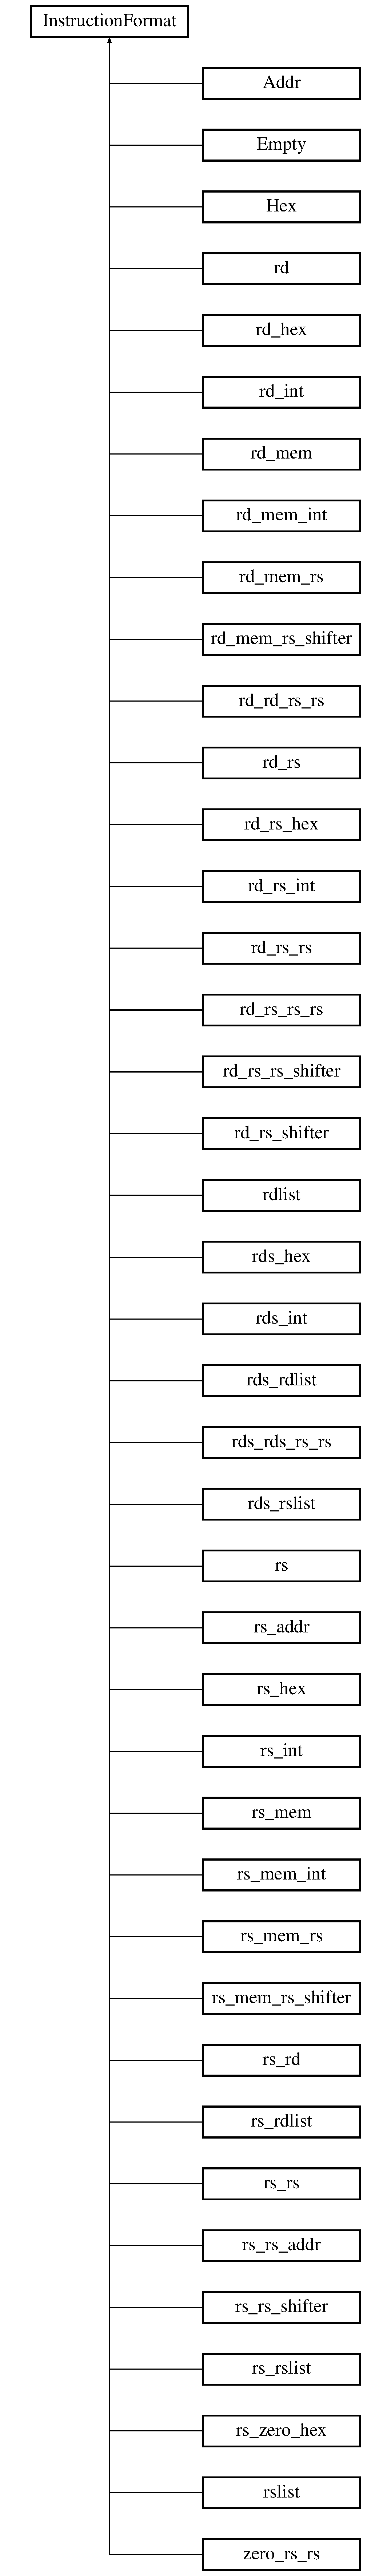
\includegraphics[height=12.000000cm]{classInstructionFormat}
\end{center}
\end{figure}
\subsection*{Public Member Functions}
\begin{DoxyCompactItemize}
\item 
virtual bool \hyperlink{classInstructionFormat_a9fdcf94dcd7d9a55ba86e7a63f04d1fe}{is\+Format} (const vector$<$ string $>$ \&operands)=0
\item 
virtual vector$<$ string $>$ \hyperlink{classInstructionFormat_a09775d3a3c22f40a0f44504664e586e4}{get\+Resource\+Inputs} (const vector$<$ string $>$ \&operands)=0
\item 
virtual vector$<$ string $>$ \hyperlink{classInstructionFormat_a95cd28ffb1bde59b67f676880ab10536}{get\+Resource\+Outputs} (const vector$<$ string $>$ \&operands)=0
\item 
virtual \hyperlink{classInstructionFormat_a104e78d49e31e4e88ac9545dbadf9f7a}{$\sim$\+Instruction\+Format} ()
\end{DoxyCompactItemize}


\subsection{Constructor \& Destructor Documentation}
\mbox{\Hypertarget{classInstructionFormat_a104e78d49e31e4e88ac9545dbadf9f7a}\label{classInstructionFormat_a104e78d49e31e4e88ac9545dbadf9f7a}} 
\index{Instruction\+Format@{Instruction\+Format}!````~Instruction\+Format@{$\sim$\+Instruction\+Format}}
\index{````~Instruction\+Format@{$\sim$\+Instruction\+Format}!Instruction\+Format@{Instruction\+Format}}
\subsubsection{\texorpdfstring{$\sim$\+Instruction\+Format()}{~InstructionFormat()}}
{\footnotesize\ttfamily virtual Instruction\+Format\+::$\sim$\+Instruction\+Format (\begin{DoxyParamCaption}{ }\end{DoxyParamCaption})\hspace{0.3cm}{\ttfamily [inline]}, {\ttfamily [virtual]}}

Virtual destructor 

\subsection{Member Function Documentation}
\mbox{\Hypertarget{classInstructionFormat_a09775d3a3c22f40a0f44504664e586e4}\label{classInstructionFormat_a09775d3a3c22f40a0f44504664e586e4}} 
\index{Instruction\+Format@{Instruction\+Format}!get\+Resource\+Inputs@{get\+Resource\+Inputs}}
\index{get\+Resource\+Inputs@{get\+Resource\+Inputs}!Instruction\+Format@{Instruction\+Format}}
\subsubsection{\texorpdfstring{get\+Resource\+Inputs()}{getResourceInputs()}}
{\footnotesize\ttfamily virtual vector$<$string$>$ Instruction\+Format\+::get\+Resource\+Inputs (\begin{DoxyParamCaption}\item[{const vector$<$ string $>$ \&}]{operands }\end{DoxyParamCaption})\hspace{0.3cm}{\ttfamily [pure virtual]}}

Returns the input resources 

Implemented in \hyperlink{classrds__rdlist_aaece2a143143616bd8a08665bde1a617}{rds\+\_\+rdlist}, \hyperlink{classrs__rdlist_a52adf024855b236f038cc7140b9f5cc9}{rs\+\_\+rdlist}, \hyperlink{classrds__rslist_a8b7009023b3cfecdd39dc36118c33069}{rds\+\_\+rslist}, \hyperlink{classrs__rslist_a6e678afc02083eaa9c815a291ca010c9}{rs\+\_\+rslist}, \hyperlink{classrdlist_a6323881f795a77f99a05cdbea09f3a8b}{rdlist}, \hyperlink{classrslist_aecc14cc02c8e8e7cc6f1ac2989083bda}{rslist}, \hyperlink{classrd__rs__rs__shifter_a6702691c38b2f3739d3c6f754f51411e}{rd\+\_\+rs\+\_\+rs\+\_\+shifter}, \hyperlink{classrs__mem__rs__shifter_a90b19d41406d19856f18fb7f96bf415c}{rs\+\_\+mem\+\_\+rs\+\_\+shifter}, \hyperlink{classrd__mem__rs__shifter_a834887022a5d0ac6ddf56df2c2966975}{rd\+\_\+mem\+\_\+rs\+\_\+shifter}, \hyperlink{classrds__rds__rs__rs_a1e5f81778283024ee7f464bde0619a78}{rds\+\_\+rds\+\_\+rs\+\_\+rs}, \hyperlink{classrd__rs__rs__rs_af94c94f5cea0acff0acd499d15b65a84}{rd\+\_\+rs\+\_\+rs\+\_\+rs}, \hyperlink{classrd__rd__rs__rs_aa04311f97ba9aae16803046e190ecc1d}{rd\+\_\+rd\+\_\+rs\+\_\+rs}, \hyperlink{classrd__rs__shifter_ae52cf6e9a846ab34fd0d248c9c4f9008}{rd\+\_\+rs\+\_\+shifter}, \hyperlink{classrs__rs__shifter_aa4407b74c1d13c32743e484733efc95d}{rs\+\_\+rs\+\_\+shifter}, \hyperlink{classrs__mem__rs_acf80e20421747fcaa4b0ae7af2db591a}{rs\+\_\+mem\+\_\+rs}, \hyperlink{classrd__mem__rs_aab55c71432b31ddd0ac1b9a89a6e29e5}{rd\+\_\+mem\+\_\+rs}, \hyperlink{classrs__mem__int_a3a1627ce0396aa81bc60b4f36e4f669f}{rs\+\_\+mem\+\_\+int}, \hyperlink{classrd__mem__int_ae5e48b6200ba20ace72f78d1baa3a2fd}{rd\+\_\+mem\+\_\+int}, \hyperlink{classrds__hex_a2f3730108e307942aeecc3b07d2b0f5c}{rds\+\_\+hex}, \hyperlink{classrds__int_a99103f5596a0efdac0644c0a3b29ab8a}{rds\+\_\+int}, \hyperlink{classrs__hex_a98b9ec3e52203665ad8375d9cd01e17f}{rs\+\_\+hex}, \hyperlink{classrs__int_a75c4c434457fcf4a2058993acf97298f}{rs\+\_\+int}, \hyperlink{classrd__rs__hex_acef60c9ce93239e4cfcdadbe65355782}{rd\+\_\+rs\+\_\+hex}, \hyperlink{classrd__rs__int_a8774c36cc600b25365a1616f4fb5f94b}{rd\+\_\+rs\+\_\+int}, \hyperlink{classrd__rs__rs_a1df3edc555878b75cbd426889c28cec0}{rd\+\_\+rs\+\_\+rs}, \hyperlink{classzero__rs__rs_a697c00ba542cb6f8f610dce7501ecab5}{zero\+\_\+rs\+\_\+rs}, \hyperlink{classrs__rs__addr_a48fbea2fd176094ecbcfac62627a5cd7}{rs\+\_\+rs\+\_\+addr}, \hyperlink{classrs__zero__hex_a4a3e207656744266c6012e58cbab5de0}{rs\+\_\+zero\+\_\+hex}, \hyperlink{classrd__hex_a4afabb7f88c944befc0cd880b2f574f1}{rd\+\_\+hex}, \hyperlink{classrs__rs_a0f171a0f2819f3980516ee0c12707f8b}{rs\+\_\+rs}, \hyperlink{classrs__rd_aae3990a01a4cc7cb32f4c1f32fffc8ac}{rs\+\_\+rd}, \hyperlink{classrd__rs_a0e0013c3f91637813f475c12f8062e3e}{rd\+\_\+rs}, \hyperlink{classrs__addr_aa0bfc19d335d4888e8fc97edb0ef248e}{rs\+\_\+addr}, \hyperlink{classrs__mem_a4296ae1f58884fe3a3d85a265a3657a8}{rs\+\_\+mem}, \hyperlink{classrd__int_a9c533c36eeee420c88f0bd7fbf631d9d}{rd\+\_\+int}, \hyperlink{classrd__mem_a0f3a8067b15d3a7a171c15e90b10f7f0}{rd\+\_\+mem}, \hyperlink{classrs_a5bac2f73d84e28ab6037a368fab75d91}{rs}, \hyperlink{classAddr_a0ed20cdb01d8b11b023fa3b5e54bab29}{Addr}, \hyperlink{classHex_aed4f7917c651fb60226466f5f5fc9f3b}{Hex}, \hyperlink{classrd_a06b5b25f6e269bb121ad8ab63283f599}{rd}, and \hyperlink{classEmpty_a8710df419a0fe47e9a66d504a6cb016f}{Empty}.

\mbox{\Hypertarget{classInstructionFormat_a95cd28ffb1bde59b67f676880ab10536}\label{classInstructionFormat_a95cd28ffb1bde59b67f676880ab10536}} 
\index{Instruction\+Format@{Instruction\+Format}!get\+Resource\+Outputs@{get\+Resource\+Outputs}}
\index{get\+Resource\+Outputs@{get\+Resource\+Outputs}!Instruction\+Format@{Instruction\+Format}}
\subsubsection{\texorpdfstring{get\+Resource\+Outputs()}{getResourceOutputs()}}
{\footnotesize\ttfamily virtual vector$<$string$>$ Instruction\+Format\+::get\+Resource\+Outputs (\begin{DoxyParamCaption}\item[{const vector$<$ string $>$ \&}]{operands }\end{DoxyParamCaption})\hspace{0.3cm}{\ttfamily [pure virtual]}}

Returns the output resources 

Implemented in \hyperlink{classrds__rdlist_a42eb3f3d04fec1d67da0b7de1d27ac10}{rds\+\_\+rdlist}, \hyperlink{classrs__rdlist_acb2773ca764d509fe6acaeaf83064b90}{rs\+\_\+rdlist}, \hyperlink{classrds__rslist_a495f7309e2936109a910d06d9d19f9f5}{rds\+\_\+rslist}, \hyperlink{classrs__rslist_aec1bc27b2d4f484cc2f2c65dd29f8db2}{rs\+\_\+rslist}, \hyperlink{classrdlist_a5757c02c361945639b7c5f11f93a5e37}{rdlist}, \hyperlink{classrslist_adc1bf6be9d82f0a616fc374023d8a636}{rslist}, \hyperlink{classrd__rs__rs__shifter_a4ec7aa9c844e62d408c8846406d854ec}{rd\+\_\+rs\+\_\+rs\+\_\+shifter}, \hyperlink{classrs__mem__rs__shifter_a798cbf0eeae065cffc3acf44a01b2221}{rs\+\_\+mem\+\_\+rs\+\_\+shifter}, \hyperlink{classrd__mem__rs__shifter_aa0e2be11d366b4dda2b50f14194ddfbf}{rd\+\_\+mem\+\_\+rs\+\_\+shifter}, \hyperlink{classrds__rds__rs__rs_a1e28d72e1c55d801ca8fecdce34db4e2}{rds\+\_\+rds\+\_\+rs\+\_\+rs}, \hyperlink{classrd__rs__rs__rs_ae8da7457b4ac57c9a2cc470ebb8da345}{rd\+\_\+rs\+\_\+rs\+\_\+rs}, \hyperlink{classrd__rd__rs__rs_a7e666988b9c7ff5fb02074575311516c}{rd\+\_\+rd\+\_\+rs\+\_\+rs}, \hyperlink{classrd__rs__shifter_aed7186be3ead5fe24d6d63eacdf817bd}{rd\+\_\+rs\+\_\+shifter}, \hyperlink{classrs__rs__shifter_a1f34f4ebe7ad98f670811d9a43629fdb}{rs\+\_\+rs\+\_\+shifter}, \hyperlink{classrs__mem__rs_ad93e4a2a21f172863e3daf317db69ad1}{rs\+\_\+mem\+\_\+rs}, \hyperlink{classrd__mem__rs_a9f22532c1535bba6776bf7051c50de0f}{rd\+\_\+mem\+\_\+rs}, \hyperlink{classrs__mem__int_a181c97b7f9f26c5a3d0b7fd7949628b4}{rs\+\_\+mem\+\_\+int}, \hyperlink{classrd__mem__int_a73d6daee8115110da422c2dc8685c6ea}{rd\+\_\+mem\+\_\+int}, \hyperlink{classrds__hex_a40821f2b6ed827019708864a90d7ee81}{rds\+\_\+hex}, \hyperlink{classrds__int_acbcdd1ee4ccce4fab70fc88878b89eb4}{rds\+\_\+int}, \hyperlink{classrs__hex_a7b4f63e180c5641a65037eff96b339f0}{rs\+\_\+hex}, \hyperlink{classrs__int_a8c83bc7081f9ff48657aaf5d7fbbaf1d}{rs\+\_\+int}, \hyperlink{classrd__rs__hex_a268da92bc87148bd3f8f5b0086a442f5}{rd\+\_\+rs\+\_\+hex}, \hyperlink{classrd__rs__int_a48f2b5901a9a74c1cad322fa4bd50f65}{rd\+\_\+rs\+\_\+int}, \hyperlink{classrd__rs__rs_ae2fd5d87f3db344ce4f8cea452ef6913}{rd\+\_\+rs\+\_\+rs}, \hyperlink{classzero__rs__rs_a8700492ca6deb31a550493e267468c4c}{zero\+\_\+rs\+\_\+rs}, \hyperlink{classrs__rs__addr_a6918ea18f88f75f349bd59c397bb5ca1}{rs\+\_\+rs\+\_\+addr}, \hyperlink{classrs__zero__hex_ade4a0e0f8aa6fe706a2bc6059c56013e}{rs\+\_\+zero\+\_\+hex}, \hyperlink{classrd__hex_a5f437d79049848b5038272a70fb09cc3}{rd\+\_\+hex}, \hyperlink{classrs__rs_ad0ceb0c23af2d485184ca1229ab27483}{rs\+\_\+rs}, \hyperlink{classrs__rd_aeb39c1906a9ccd080b21dda0f711b6ed}{rs\+\_\+rd}, \hyperlink{classrd__rs_a52ac7e75ebef24ff1ac211d8dd0e4f5d}{rd\+\_\+rs}, \hyperlink{classrs__addr_ae38e946613927e43fc9ec274386978f7}{rs\+\_\+addr}, \hyperlink{classrs__mem_a43c0456a0a59e714915e9d7b14e2246b}{rs\+\_\+mem}, \hyperlink{classrd__int_a3728611aa3701f90fdaca2e63198ff80}{rd\+\_\+int}, \hyperlink{classrd__mem_a84b92866d710443ed821459840541f53}{rd\+\_\+mem}, \hyperlink{classrs_aa6a9c35c6eb4b5f8cfc8c41484b5a0b9}{rs}, \hyperlink{classAddr_aa42b861112df7333d93b3dd242e6621b}{Addr}, \hyperlink{classHex_a6fa1b11eff40eafe79e7291864915dd7}{Hex}, \hyperlink{classrd_a148dde5e9f8d3c68d5563dd8ec2c1bff}{rd}, and \hyperlink{classEmpty_a2952fa936d380f530b232bce35d337be}{Empty}.

\mbox{\Hypertarget{classInstructionFormat_a9fdcf94dcd7d9a55ba86e7a63f04d1fe}\label{classInstructionFormat_a9fdcf94dcd7d9a55ba86e7a63f04d1fe}} 
\index{Instruction\+Format@{Instruction\+Format}!is\+Format@{is\+Format}}
\index{is\+Format@{is\+Format}!Instruction\+Format@{Instruction\+Format}}
\subsubsection{\texorpdfstring{is\+Format()}{isFormat()}}
{\footnotesize\ttfamily virtual bool Instruction\+Format\+::is\+Format (\begin{DoxyParamCaption}\item[{const vector$<$ string $>$ \&}]{operands }\end{DoxyParamCaption})\hspace{0.3cm}{\ttfamily [pure virtual]}}

Returns true if operands match the format 

Implemented in \hyperlink{classrds__rdlist_ad3df9613000e862de6ee574509e1bf0c}{rds\+\_\+rdlist}, \hyperlink{classrs__rdlist_a3bf959757fd3abfc635485e85471dce4}{rs\+\_\+rdlist}, \hyperlink{classrds__rslist_a3b1c315345a6e795534f04788f810f31}{rds\+\_\+rslist}, \hyperlink{classrs__rslist_a761f3da0f588fcd4e93e446c98d4c263}{rs\+\_\+rslist}, \hyperlink{classrdlist_a14fd300b1148e07a48853f79cc8bdb2a}{rdlist}, \hyperlink{classrslist_aaa2d2aa941041c08369254f21e8846b7}{rslist}, \hyperlink{classrd__rs__rs__shifter_aa60a168e3fb236635bab054c85a8ef0e}{rd\+\_\+rs\+\_\+rs\+\_\+shifter}, \hyperlink{classrs__mem__rs__shifter_a8499ed65e4e65d8ffc0a15f4216de118}{rs\+\_\+mem\+\_\+rs\+\_\+shifter}, \hyperlink{classrd__mem__rs__shifter_a483c16d44defe4965af7850ba9529cd7}{rd\+\_\+mem\+\_\+rs\+\_\+shifter}, \hyperlink{classrds__rds__rs__rs_acabfdee1b6f208c2f141fdef6ba45c38}{rds\+\_\+rds\+\_\+rs\+\_\+rs}, \hyperlink{classrd__rs__rs__rs_adb8dd9ede11ef73c82f331d8ab25ad02}{rd\+\_\+rs\+\_\+rs\+\_\+rs}, \hyperlink{classrd__rd__rs__rs_a66f9df0e42a4e8fd37d4182a22321602}{rd\+\_\+rd\+\_\+rs\+\_\+rs}, \hyperlink{classrd__rs__shifter_a78e9526cc76d33f8dbfe614733ee3564}{rd\+\_\+rs\+\_\+shifter}, \hyperlink{classrs__rs__shifter_a0d8deef39f7613736c69008bedfb0265}{rs\+\_\+rs\+\_\+shifter}, \hyperlink{classrs__mem__rs_abf2731ea9f051772088147dcecb111dc}{rs\+\_\+mem\+\_\+rs}, \hyperlink{classrd__mem__rs_ad9242fac1115765f6cf9f6cf632d8d25}{rd\+\_\+mem\+\_\+rs}, \hyperlink{classrs__mem__int_a49a72c354a4ff7e9dda94f75810de59f}{rs\+\_\+mem\+\_\+int}, \hyperlink{classrd__mem__int_a7cf061c18744708846c625ccf275fc3f}{rd\+\_\+mem\+\_\+int}, \hyperlink{classrds__hex_afcf9c40012c4a3d90cc5811cca063244}{rds\+\_\+hex}, \hyperlink{classrds__int_ac34d1eca9d3ada3e8c2d2b063216d955}{rds\+\_\+int}, \hyperlink{classrs__hex_abd5955b23a014a84f32125fb9d6a75c8}{rs\+\_\+hex}, \hyperlink{classrs__int_ad8660fae74d3763a5068b22a79ffdd92}{rs\+\_\+int}, \hyperlink{classrd__rs__hex_ae39510e90b575861fdaa315308ef8638}{rd\+\_\+rs\+\_\+hex}, \hyperlink{classrd__rs__int_a0950cf3d4598c079cf88117d41fab7ea}{rd\+\_\+rs\+\_\+int}, \hyperlink{classrd__rs__rs_a9f92e9d08e1cc714507225a0fd961aba}{rd\+\_\+rs\+\_\+rs}, \hyperlink{classzero__rs__rs_a0a3cc74b189c29a3665a4ab80e3b0aba}{zero\+\_\+rs\+\_\+rs}, \hyperlink{classrs__rs__addr_a8e43a85fbdd3849d11088baa3db70185}{rs\+\_\+rs\+\_\+addr}, \hyperlink{classrs__zero__hex_ab1086f903e313eff8021b5edd83af9eb}{rs\+\_\+zero\+\_\+hex}, \hyperlink{classrd__hex_a9e91ce0f836feac13681445ef741edf2}{rd\+\_\+hex}, \hyperlink{classrs__rs_a1c8ae600e477053cc3eab27edebe6b53}{rs\+\_\+rs}, \hyperlink{classrs__rd_a982dd920345cfe325ee486e099640359}{rs\+\_\+rd}, \hyperlink{classrd__rs_a11e48da979b9ac645d90fc9bbdbfc444}{rd\+\_\+rs}, \hyperlink{classrs__addr_a49101844a8143d3ad6be1fc1435bc719}{rs\+\_\+addr}, \hyperlink{classrs__mem_a81ea68538cb372c59b98d269fb0708c5}{rs\+\_\+mem}, \hyperlink{classrd__int_aded49d47c21e49d1f71a9531d1c600b2}{rd\+\_\+int}, \hyperlink{classrd__mem_a1326e4c5e3a7f263d5dc850b0d32962f}{rd\+\_\+mem}, \hyperlink{classrs_a6b8aa703ea54d95ddb7badc5c95c29f5}{rs}, \hyperlink{classAddr_aff6fd4bf7c93990b1427843fff9069ed}{Addr}, \hyperlink{classHex_aabeb457d36ac38c382cf3735a9b32648}{Hex}, \hyperlink{classrd_a8a37174ea94c394743494d3e735d6363}{rd}, and \hyperlink{classEmpty_a2fce1c7e9e73a489c8a79a4046ae45b0}{Empty}.



The documentation for this class was generated from the following file\+:\begin{DoxyCompactItemize}
\item 
src/\hyperlink{InstructionFormat_8h}{Instruction\+Format.\+h}\end{DoxyCompactItemize}

\hypertarget{classInstructionType}{}\section{Instruction\+Type Class Reference}
\label{classInstructionType}\index{Instruction\+Type@{Instruction\+Type}}


{\ttfamily \#include $<$Instruction\+Type.\+h$>$}

Inheritance diagram for Instruction\+Type\+:\begin{figure}[H]
\begin{center}
\leavevmode
\includegraphics[height=12.000000cm]{classInstructionType}
\end{center}
\end{figure}
\subsection*{Public Member Functions}
\begin{DoxyCompactItemize}
\item 
virtual bool \hyperlink{classInstructionType_aa3d2c042a4109b1d96dc0d7f20916ba3}{is\+Load} ()
\item 
virtual bool \hyperlink{classInstructionType_aa81de3619fb9d88f52d7d8104f9ac188}{is\+Store} ()
\item 
virtual bool \hyperlink{classInstructionType_ad49a039e3b57e3b7b369a7c0c6c0932b}{is\+Call} ()
\item 
virtual bool \hyperlink{classInstructionType_a15b0f034f3536f0bc525550406e1d7c6}{is\+Return} ()
\item 
virtual bool \hyperlink{classInstructionType_a145a4e04a4db8a0ecf9e4b35b2403ed3}{is\+Unconditional\+Jump} ()
\item 
virtual bool \hyperlink{classInstructionType_a3655591172fa6acbf7b9888e879b551d}{is\+Conditional\+Jump} ()
\item 
\hyperlink{classDAAInstruction}{D\+A\+A\+Instruction} $\ast$ \hyperlink{classInstructionType_aed61394dd1528a3a68c09bef157e6da8}{get\+D\+A\+A\+Instruction} ()
\item 
int \hyperlink{classInstructionType_a737bd48f4e73da7c3a52faa052d9edfe}{get\+Latency} ()
\item 
virtual bool \hyperlink{classInstructionType_a5b28d5b2e495222817facca7b8826975}{is\+Predicated} ()
\item 
virtual bool \hyperlink{classInstructionType_ab4c4569a2cafed0655f95d9a20bd8ea1}{is\+Word} ()
\item 
virtual bool \hyperlink{classInstructionType_ada75c9091ab7e6b4b9a7df984288d1f8}{is\+Basic} ()
\item 
virtual int \hyperlink{classInstructionType_a40c94ccf0b13f186524e06972f08bca3}{get\+Size\+Of\+Memory\+Access} ()
\item 
bool \hyperlink{classInstructionType_a0711bca7a3ca0a21ff6b9ae940c13acf}{check\+Format} (const vector$<$ string $>$ \&operands)
\item 
string \hyperlink{classInstructionType_adf12516c59a85e8032770feec2e1dcae}{get\+Resource\+Functional\+Unit} ()
\item 
vector$<$ string $>$ \hyperlink{classInstructionType_acce0f34d0675a5e29518ecba9bcb13c1}{get\+Resource\+Inputs} (const vector$<$ string $>$ \&operands)
\item 
vector$<$ string $>$ \hyperlink{classInstructionType_a96e341d8911549b19e8d975297e3e131}{get\+Resource\+Outputs} (const vector$<$ string $>$ \&operands)
\item 
virtual \hyperlink{classInstructionType_ae3415fa195f43d8fd0c4c66fab307e3d}{$\sim$\+Instruction\+Type} ()
\end{DoxyCompactItemize}
\subsection*{Protected Attributes}
\begin{DoxyCompactItemize}
\item 
string \hyperlink{classInstructionType_a5163498ca8a68d727c6c89cd443a37f8}{functional\+Unit}
\item 
set$<$ \hyperlink{classInstructionFormat}{Instruction\+Format} $\ast$ $>$ \hyperlink{classInstructionType_a039493f9dcd605e25bb96ac3f510a501}{formats}
\item 
\hyperlink{classDAAInstruction}{D\+A\+A\+Instruction} $\ast$ \hyperlink{classInstructionType_a7dfb488bd47f9168dc5fa1604a18c6c4}{addr\+Analysis\+Instruction}
\item 
int \hyperlink{classInstructionType_a99de20a7ccac1417a3e777ff25dfe3ed}{latency}
\end{DoxyCompactItemize}


\subsection{Constructor \& Destructor Documentation}
\mbox{\Hypertarget{classInstructionType_ae3415fa195f43d8fd0c4c66fab307e3d}\label{classInstructionType_ae3415fa195f43d8fd0c4c66fab307e3d}} 
\index{Instruction\+Type@{Instruction\+Type}!````~Instruction\+Type@{$\sim$\+Instruction\+Type}}
\index{````~Instruction\+Type@{$\sim$\+Instruction\+Type}!Instruction\+Type@{Instruction\+Type}}
\subsubsection{\texorpdfstring{$\sim$\+Instruction\+Type()}{~InstructionType()}}
{\footnotesize\ttfamily virtual Instruction\+Type\+::$\sim$\+Instruction\+Type (\begin{DoxyParamCaption}{ }\end{DoxyParamCaption})\hspace{0.3cm}{\ttfamily [virtual]}}

Virtual destructor 

\subsection{Member Function Documentation}
\mbox{\Hypertarget{classInstructionType_a0711bca7a3ca0a21ff6b9ae940c13acf}\label{classInstructionType_a0711bca7a3ca0a21ff6b9ae940c13acf}} 
\index{Instruction\+Type@{Instruction\+Type}!check\+Format@{check\+Format}}
\index{check\+Format@{check\+Format}!Instruction\+Type@{Instruction\+Type}}
\subsubsection{\texorpdfstring{check\+Format()}{checkFormat()}}
{\footnotesize\ttfamily bool Instruction\+Type\+::check\+Format (\begin{DoxyParamCaption}\item[{const vector$<$ string $>$ \&}]{operands }\end{DoxyParamCaption})}

Returns true if one and only one \hyperlink{classInstructionFormat}{Instruction\+Format} corresponds to the operands \mbox{\Hypertarget{classInstructionType_aed61394dd1528a3a68c09bef157e6da8}\label{classInstructionType_aed61394dd1528a3a68c09bef157e6da8}} 
\index{Instruction\+Type@{Instruction\+Type}!get\+D\+A\+A\+Instruction@{get\+D\+A\+A\+Instruction}}
\index{get\+D\+A\+A\+Instruction@{get\+D\+A\+A\+Instruction}!Instruction\+Type@{Instruction\+Type}}
\subsubsection{\texorpdfstring{get\+D\+A\+A\+Instruction()}{getDAAInstruction()}}
{\footnotesize\ttfamily \hyperlink{classDAAInstruction}{D\+A\+A\+Instruction}$\ast$ Instruction\+Type\+::get\+D\+A\+A\+Instruction (\begin{DoxyParamCaption}{ }\end{DoxyParamCaption})}

Returns the address analysis instruction \mbox{\Hypertarget{classInstructionType_a737bd48f4e73da7c3a52faa052d9edfe}\label{classInstructionType_a737bd48f4e73da7c3a52faa052d9edfe}} 
\index{Instruction\+Type@{Instruction\+Type}!get\+Latency@{get\+Latency}}
\index{get\+Latency@{get\+Latency}!Instruction\+Type@{Instruction\+Type}}
\subsubsection{\texorpdfstring{get\+Latency()}{getLatency()}}
{\footnotesize\ttfamily int Instruction\+Type\+::get\+Latency (\begin{DoxyParamCaption}{ }\end{DoxyParamCaption})}

Returns the latency of the instruction \mbox{\Hypertarget{classInstructionType_adf12516c59a85e8032770feec2e1dcae}\label{classInstructionType_adf12516c59a85e8032770feec2e1dcae}} 
\index{Instruction\+Type@{Instruction\+Type}!get\+Resource\+Functional\+Unit@{get\+Resource\+Functional\+Unit}}
\index{get\+Resource\+Functional\+Unit@{get\+Resource\+Functional\+Unit}!Instruction\+Type@{Instruction\+Type}}
\subsubsection{\texorpdfstring{get\+Resource\+Functional\+Unit()}{getResourceFunctionalUnit()}}
{\footnotesize\ttfamily string Instruction\+Type\+::get\+Resource\+Functional\+Unit (\begin{DoxyParamCaption}{ }\end{DoxyParamCaption})}

Returns the functional\+Units \mbox{\Hypertarget{classInstructionType_acce0f34d0675a5e29518ecba9bcb13c1}\label{classInstructionType_acce0f34d0675a5e29518ecba9bcb13c1}} 
\index{Instruction\+Type@{Instruction\+Type}!get\+Resource\+Inputs@{get\+Resource\+Inputs}}
\index{get\+Resource\+Inputs@{get\+Resource\+Inputs}!Instruction\+Type@{Instruction\+Type}}
\subsubsection{\texorpdfstring{get\+Resource\+Inputs()}{getResourceInputs()}}
{\footnotesize\ttfamily vector$<$string$>$ Instruction\+Type\+::get\+Resource\+Inputs (\begin{DoxyParamCaption}\item[{const vector$<$ string $>$ \&}]{operands }\end{DoxyParamCaption})}

Returns the input resources \mbox{\Hypertarget{classInstructionType_a96e341d8911549b19e8d975297e3e131}\label{classInstructionType_a96e341d8911549b19e8d975297e3e131}} 
\index{Instruction\+Type@{Instruction\+Type}!get\+Resource\+Outputs@{get\+Resource\+Outputs}}
\index{get\+Resource\+Outputs@{get\+Resource\+Outputs}!Instruction\+Type@{Instruction\+Type}}
\subsubsection{\texorpdfstring{get\+Resource\+Outputs()}{getResourceOutputs()}}
{\footnotesize\ttfamily vector$<$string$>$ Instruction\+Type\+::get\+Resource\+Outputs (\begin{DoxyParamCaption}\item[{const vector$<$ string $>$ \&}]{operands }\end{DoxyParamCaption})}

Returns the output resources \mbox{\Hypertarget{classInstructionType_a40c94ccf0b13f186524e06972f08bca3}\label{classInstructionType_a40c94ccf0b13f186524e06972f08bca3}} 
\index{Instruction\+Type@{Instruction\+Type}!get\+Size\+Of\+Memory\+Access@{get\+Size\+Of\+Memory\+Access}}
\index{get\+Size\+Of\+Memory\+Access@{get\+Size\+Of\+Memory\+Access}!Instruction\+Type@{Instruction\+Type}}
\subsubsection{\texorpdfstring{get\+Size\+Of\+Memory\+Access()}{getSizeOfMemoryAccess()}}
{\footnotesize\ttfamily virtual int Instruction\+Type\+::get\+Size\+Of\+Memory\+Access (\begin{DoxyParamCaption}{ }\end{DoxyParamCaption})\hspace{0.3cm}{\ttfamily [virtual]}}

Returns the size of the memory access in bytes, if the instruction is a load/store and 0 otherwise 

Reimplemented in \hyperlink{classPredicatedLoad_a0f4d0a0830281e9f87c733eb253a1a5e}{Predicated\+Load}, \hyperlink{classPredicatedStore_a79f5e84001443055c5ae0547ec337759}{Predicated\+Store}, \hyperlink{classLoad_a35d504d74dfa9ea02ae719f41dd766a8}{Load}, and \hyperlink{classStore_a1b788e1fc3364a4eb304a2611ad37415}{Store}.

\mbox{\Hypertarget{classInstructionType_ada75c9091ab7e6b4b9a7df984288d1f8}\label{classInstructionType_ada75c9091ab7e6b4b9a7df984288d1f8}} 
\index{Instruction\+Type@{Instruction\+Type}!is\+Basic@{is\+Basic}}
\index{is\+Basic@{is\+Basic}!Instruction\+Type@{Instruction\+Type}}
\subsubsection{\texorpdfstring{is\+Basic()}{isBasic()}}
{\footnotesize\ttfamily virtual bool Instruction\+Type\+::is\+Basic (\begin{DoxyParamCaption}{ }\end{DoxyParamCaption})\hspace{0.3cm}{\ttfamily [virtual]}}

Returns true if the instruction is a basic instruction 

Reimplemented in \hyperlink{classPredicatedBasic_ad3f2e7d2feaef666dd784fcae0f03125}{Predicated\+Basic}, and \hyperlink{classBasic_a3ab68a71a2c405d7e14a11a8ce24fd07}{Basic}.

\mbox{\Hypertarget{classInstructionType_ad49a039e3b57e3b7b369a7c0c6c0932b}\label{classInstructionType_ad49a039e3b57e3b7b369a7c0c6c0932b}} 
\index{Instruction\+Type@{Instruction\+Type}!is\+Call@{is\+Call}}
\index{is\+Call@{is\+Call}!Instruction\+Type@{Instruction\+Type}}
\subsubsection{\texorpdfstring{is\+Call()}{isCall()}}
{\footnotesize\ttfamily virtual bool Instruction\+Type\+::is\+Call (\begin{DoxyParamCaption}{ }\end{DoxyParamCaption})\hspace{0.3cm}{\ttfamily [virtual]}}

Returns true if the instruction is a call instruction 

Reimplemented in \hyperlink{classCall_a2f33492c84abcac87ff5e388535f6cfb}{Call}.

\mbox{\Hypertarget{classInstructionType_a3655591172fa6acbf7b9888e879b551d}\label{classInstructionType_a3655591172fa6acbf7b9888e879b551d}} 
\index{Instruction\+Type@{Instruction\+Type}!is\+Conditional\+Jump@{is\+Conditional\+Jump}}
\index{is\+Conditional\+Jump@{is\+Conditional\+Jump}!Instruction\+Type@{Instruction\+Type}}
\subsubsection{\texorpdfstring{is\+Conditional\+Jump()}{isConditionalJump()}}
{\footnotesize\ttfamily virtual bool Instruction\+Type\+::is\+Conditional\+Jump (\begin{DoxyParamCaption}{ }\end{DoxyParamCaption})\hspace{0.3cm}{\ttfamily [virtual]}}

Returns true if the instruction is a Conditionnal Jump instruction 

Reimplemented in \hyperlink{classConditionalJump_a2341c5b034b189c24b858651a51d6dba}{Conditional\+Jump}.

\mbox{\Hypertarget{classInstructionType_aa3d2c042a4109b1d96dc0d7f20916ba3}\label{classInstructionType_aa3d2c042a4109b1d96dc0d7f20916ba3}} 
\index{Instruction\+Type@{Instruction\+Type}!is\+Load@{is\+Load}}
\index{is\+Load@{is\+Load}!Instruction\+Type@{Instruction\+Type}}
\subsubsection{\texorpdfstring{is\+Load()}{isLoad()}}
{\footnotesize\ttfamily virtual bool Instruction\+Type\+::is\+Load (\begin{DoxyParamCaption}{ }\end{DoxyParamCaption})\hspace{0.3cm}{\ttfamily [virtual]}}

Returns true if the instruction is a load instruction 

Reimplemented in \hyperlink{classPredicatedLoad_a6eba0b6ea212b012d2015fb023804fc3}{Predicated\+Load}, and \hyperlink{classLoad_aa7fbffafad6cbfa1b9866f6d09cc7e30}{Load}.

\mbox{\Hypertarget{classInstructionType_a5b28d5b2e495222817facca7b8826975}\label{classInstructionType_a5b28d5b2e495222817facca7b8826975}} 
\index{Instruction\+Type@{Instruction\+Type}!is\+Predicated@{is\+Predicated}}
\index{is\+Predicated@{is\+Predicated}!Instruction\+Type@{Instruction\+Type}}
\subsubsection{\texorpdfstring{is\+Predicated()}{isPredicated()}}
{\footnotesize\ttfamily virtual bool Instruction\+Type\+::is\+Predicated (\begin{DoxyParamCaption}{ }\end{DoxyParamCaption})\hspace{0.3cm}{\ttfamily [virtual]}}

Returns true if the instruction is Predicated (with a condition) 

Reimplemented in \hyperlink{classPredicatedLoad_aebf98efc7d6d09ec1d8f9c578a65e156}{Predicated\+Load}, \hyperlink{classPredicatedStore_a204c4cac7241d1d1b61719c5fcbc6512}{Predicated\+Store}, and \hyperlink{classPredicatedBasic_aa63e9f18308f45cc3f74e27d9db3ef29}{Predicated\+Basic}.

\mbox{\Hypertarget{classInstructionType_a15b0f034f3536f0bc525550406e1d7c6}\label{classInstructionType_a15b0f034f3536f0bc525550406e1d7c6}} 
\index{Instruction\+Type@{Instruction\+Type}!is\+Return@{is\+Return}}
\index{is\+Return@{is\+Return}!Instruction\+Type@{Instruction\+Type}}
\subsubsection{\texorpdfstring{is\+Return()}{isReturn()}}
{\footnotesize\ttfamily virtual bool Instruction\+Type\+::is\+Return (\begin{DoxyParamCaption}{ }\end{DoxyParamCaption})\hspace{0.3cm}{\ttfamily [virtual]}}

Returns true if the instruction is a return instruction 

Reimplemented in \hyperlink{classReturn_ad3412361560f4acdb1e4f73ab65d3bc7}{Return}.

\mbox{\Hypertarget{classInstructionType_aa81de3619fb9d88f52d7d8104f9ac188}\label{classInstructionType_aa81de3619fb9d88f52d7d8104f9ac188}} 
\index{Instruction\+Type@{Instruction\+Type}!is\+Store@{is\+Store}}
\index{is\+Store@{is\+Store}!Instruction\+Type@{Instruction\+Type}}
\subsubsection{\texorpdfstring{is\+Store()}{isStore()}}
{\footnotesize\ttfamily virtual bool Instruction\+Type\+::is\+Store (\begin{DoxyParamCaption}{ }\end{DoxyParamCaption})\hspace{0.3cm}{\ttfamily [virtual]}}

Returns true if the instruction is a store instruction 

Reimplemented in \hyperlink{classPredicatedStore_ada88354c4a4838c8ff5fa7b225f8a751}{Predicated\+Store}, and \hyperlink{classStore_a773c447c4ac4b781ea6d18d91ff3dd50}{Store}.

\mbox{\Hypertarget{classInstructionType_a145a4e04a4db8a0ecf9e4b35b2403ed3}\label{classInstructionType_a145a4e04a4db8a0ecf9e4b35b2403ed3}} 
\index{Instruction\+Type@{Instruction\+Type}!is\+Unconditional\+Jump@{is\+Unconditional\+Jump}}
\index{is\+Unconditional\+Jump@{is\+Unconditional\+Jump}!Instruction\+Type@{Instruction\+Type}}
\subsubsection{\texorpdfstring{is\+Unconditional\+Jump()}{isUnconditionalJump()}}
{\footnotesize\ttfamily virtual bool Instruction\+Type\+::is\+Unconditional\+Jump (\begin{DoxyParamCaption}{ }\end{DoxyParamCaption})\hspace{0.3cm}{\ttfamily [virtual]}}

Returns true if the instruction is a Unconditionnal Jump instruction 

Reimplemented in \hyperlink{classUnconditionalJump_ab4588132d702a35f1dc1102dacba2be5}{Unconditional\+Jump}.

\mbox{\Hypertarget{classInstructionType_ab4c4569a2cafed0655f95d9a20bd8ea1}\label{classInstructionType_ab4c4569a2cafed0655f95d9a20bd8ea1}} 
\index{Instruction\+Type@{Instruction\+Type}!is\+Word@{is\+Word}}
\index{is\+Word@{is\+Word}!Instruction\+Type@{Instruction\+Type}}
\subsubsection{\texorpdfstring{is\+Word()}{isWord()}}
{\footnotesize\ttfamily virtual bool Instruction\+Type\+::is\+Word (\begin{DoxyParamCaption}{ }\end{DoxyParamCaption})\hspace{0.3cm}{\ttfamily [virtual]}}

Returns true if the instruction is a \hyperlink{classWord}{Word} 

Reimplemented in \hyperlink{classWord_a2dde02496b26f4c78881259cb44f70e5}{Word}.



\subsection{Member Data Documentation}
\mbox{\Hypertarget{classInstructionType_a7dfb488bd47f9168dc5fa1604a18c6c4}\label{classInstructionType_a7dfb488bd47f9168dc5fa1604a18c6c4}} 
\index{Instruction\+Type@{Instruction\+Type}!addr\+Analysis\+Instruction@{addr\+Analysis\+Instruction}}
\index{addr\+Analysis\+Instruction@{addr\+Analysis\+Instruction}!Instruction\+Type@{Instruction\+Type}}
\subsubsection{\texorpdfstring{addr\+Analysis\+Instruction}{addrAnalysisInstruction}}
{\footnotesize\ttfamily \hyperlink{classDAAInstruction}{D\+A\+A\+Instruction}$\ast$ Instruction\+Type\+::addr\+Analysis\+Instruction\hspace{0.3cm}{\ttfamily [protected]}}

\mbox{\Hypertarget{classInstructionType_a039493f9dcd605e25bb96ac3f510a501}\label{classInstructionType_a039493f9dcd605e25bb96ac3f510a501}} 
\index{Instruction\+Type@{Instruction\+Type}!formats@{formats}}
\index{formats@{formats}!Instruction\+Type@{Instruction\+Type}}
\subsubsection{\texorpdfstring{formats}{formats}}
{\footnotesize\ttfamily set$<$\hyperlink{classInstructionFormat}{Instruction\+Format}$\ast$$>$ Instruction\+Type\+::formats\hspace{0.3cm}{\ttfamily [protected]}}

\mbox{\Hypertarget{classInstructionType_a5163498ca8a68d727c6c89cd443a37f8}\label{classInstructionType_a5163498ca8a68d727c6c89cd443a37f8}} 
\index{Instruction\+Type@{Instruction\+Type}!functional\+Unit@{functional\+Unit}}
\index{functional\+Unit@{functional\+Unit}!Instruction\+Type@{Instruction\+Type}}
\subsubsection{\texorpdfstring{functional\+Unit}{functionalUnit}}
{\footnotesize\ttfamily string Instruction\+Type\+::functional\+Unit\hspace{0.3cm}{\ttfamily [protected]}}

\mbox{\Hypertarget{classInstructionType_a99de20a7ccac1417a3e777ff25dfe3ed}\label{classInstructionType_a99de20a7ccac1417a3e777ff25dfe3ed}} 
\index{Instruction\+Type@{Instruction\+Type}!latency@{latency}}
\index{latency@{latency}!Instruction\+Type@{Instruction\+Type}}
\subsubsection{\texorpdfstring{latency}{latency}}
{\footnotesize\ttfamily int Instruction\+Type\+::latency\hspace{0.3cm}{\ttfamily [protected]}}



The documentation for this class was generated from the following file\+:\begin{DoxyCompactItemize}
\item 
src/\hyperlink{InstructionType_8h}{Instruction\+Type.\+h}\end{DoxyCompactItemize}

\input{classKillOp1}
\input{classKillOp2}
\input{classLi}
\hypertarget{classLoad}{}\section{Load Class Reference}
\label{classLoad}\index{Load@{Load}}


{\ttfamily \#include $<$Instruction\+Type.\+h$>$}

Inheritance diagram for Load\+:\begin{figure}[H]
\begin{center}
\leavevmode
\includegraphics[height=2.000000cm]{classLoad}
\end{center}
\end{figure}
\subsection*{Public Member Functions}
\begin{DoxyCompactItemize}
\item 
\hyperlink{classLoad_a31df9cdc72b2e48362ee6c29b7fdbc96}{Load} (int size, const string \&fu, const set$<$ \hyperlink{classInstructionFormat}{Instruction\+Format} $\ast$$>$ \&f, \hyperlink{classDAAInstruction}{D\+A\+A\+Instruction} $\ast$daainstr, int lat)
\item 
bool \hyperlink{classLoad_aa7fbffafad6cbfa1b9866f6d09cc7e30}{is\+Load} ()
\item 
int \hyperlink{classLoad_a35d504d74dfa9ea02ae719f41dd766a8}{get\+Size\+Of\+Memory\+Access} ()
\end{DoxyCompactItemize}
\subsection*{Additional Inherited Members}


\subsection{Constructor \& Destructor Documentation}
\mbox{\Hypertarget{classLoad_a31df9cdc72b2e48362ee6c29b7fdbc96}\label{classLoad_a31df9cdc72b2e48362ee6c29b7fdbc96}} 
\index{Load@{Load}!Load@{Load}}
\index{Load@{Load}!Load@{Load}}
\subsubsection{\texorpdfstring{Load()}{Load()}}
{\footnotesize\ttfamily Load\+::\+Load (\begin{DoxyParamCaption}\item[{int}]{size,  }\item[{const string \&}]{fu,  }\item[{const set$<$ \hyperlink{classInstructionFormat}{Instruction\+Format} $\ast$$>$ \&}]{f,  }\item[{\hyperlink{classDAAInstruction}{D\+A\+A\+Instruction} $\ast$}]{daainstr,  }\item[{int}]{lat }\end{DoxyParamCaption})}



\subsection{Member Function Documentation}
\mbox{\Hypertarget{classLoad_a35d504d74dfa9ea02ae719f41dd766a8}\label{classLoad_a35d504d74dfa9ea02ae719f41dd766a8}} 
\index{Load@{Load}!get\+Size\+Of\+Memory\+Access@{get\+Size\+Of\+Memory\+Access}}
\index{get\+Size\+Of\+Memory\+Access@{get\+Size\+Of\+Memory\+Access}!Load@{Load}}
\subsubsection{\texorpdfstring{get\+Size\+Of\+Memory\+Access()}{getSizeOfMemoryAccess()}}
{\footnotesize\ttfamily int Load\+::get\+Size\+Of\+Memory\+Access (\begin{DoxyParamCaption}{ }\end{DoxyParamCaption})\hspace{0.3cm}{\ttfamily [virtual]}}

Returns the size of the memory access in bytes, if the instruction is a load/store and 0 otherwise 

Reimplemented from \hyperlink{classInstructionType_a40c94ccf0b13f186524e06972f08bca3}{Instruction\+Type}.

\mbox{\Hypertarget{classLoad_aa7fbffafad6cbfa1b9866f6d09cc7e30}\label{classLoad_aa7fbffafad6cbfa1b9866f6d09cc7e30}} 
\index{Load@{Load}!is\+Load@{is\+Load}}
\index{is\+Load@{is\+Load}!Load@{Load}}
\subsubsection{\texorpdfstring{is\+Load()}{isLoad()}}
{\footnotesize\ttfamily bool Load\+::is\+Load (\begin{DoxyParamCaption}{ }\end{DoxyParamCaption})\hspace{0.3cm}{\ttfamily [virtual]}}

Returns true if the instruction is a load instruction 

Reimplemented from \hyperlink{classInstructionType_aa3d2c042a4109b1d96dc0d7f20916ba3}{Instruction\+Type}.



The documentation for this class was generated from the following file\+:\begin{DoxyCompactItemize}
\item 
src/\hyperlink{InstructionType_8h}{Instruction\+Type.\+h}\end{DoxyCompactItemize}

\hypertarget{classLui}{}\section{Lui Class Reference}
\label{classLui}\index{Lui@{Lui}}


{\ttfamily \#include $<$D\+A\+A\+Instruction\+\_\+\+M\+I\+P\+S.\+h$>$}

Inheritance diagram for Lui\+:\begin{figure}[H]
\begin{center}
\leavevmode
\includegraphics[height=2.000000cm]{classLui}
\end{center}
\end{figure}
\subsection*{Public Member Functions}
\begin{DoxyCompactItemize}
\item 
void \hyperlink{classLui_acdaa22ad7bf3485619585ea8c6adbda4}{simulate} (vector$<$ string $>$ \&, vector$<$ bool $>$ \&, \hyperlink{DAAInstruction_8h_a1b0e70ac1a04f06c8132055ed01f589f}{stack\+Type} \&vstack, \hyperlink{DAAInstruction_8h_ac5cb793e9dac3fa9693da78b7e29ab30}{stack\+Prec\+Type} \&v\+Stack\+Precision, const string \&)
\end{DoxyCompactItemize}
\subsection*{Additional Inherited Members}


\subsection{Detailed Description}


 \subsubsection*{Specific \hyperlink{classLoad}{Load} Instructions }

\subsubsection*{L\+UI (\hyperlink{classLoad}{Load} Upper Immediate) }

\subsection{Member Function Documentation}
\mbox{\Hypertarget{classLui_acdaa22ad7bf3485619585ea8c6adbda4}\label{classLui_acdaa22ad7bf3485619585ea8c6adbda4}} 
\index{Lui@{Lui}!simulate@{simulate}}
\index{simulate@{simulate}!Lui@{Lui}}
\subsubsection{\texorpdfstring{simulate()}{simulate()}}
{\footnotesize\ttfamily void Lui\+::simulate (\begin{DoxyParamCaption}\item[{vector$<$ string $>$ \&}]{regs,  }\item[{vector$<$ bool $>$ \&}]{precision,  }\item[{\hyperlink{DAAInstruction_8h_a1b0e70ac1a04f06c8132055ed01f589f}{stack\+Type} \&}]{vstack,  }\item[{\hyperlink{DAAInstruction_8h_ac5cb793e9dac3fa9693da78b7e29ab30}{stack\+Prec\+Type} \&}]{v\+Stack\+Precision,  }\item[{const string \&}]{asm\+Instr }\end{DoxyParamCaption})\hspace{0.3cm}{\ttfamily [virtual]}}

An instruction must implement a method simulate to compute the state of registers after its execution.

regs contains the contents of the machine registers before the simulation of the instruction. In case some computation can be done on register contents, simulate keeps the computation in textual format (ex\+: \char`\"{}sp+4\char`\"{}). String \char`\"{}$\ast$\char`\"{} denote that nothing is known about the register (and then the precision for the given register is set to false).

asm\+Instr (input) contains the textual representation of the instruction

precision contains information on registers whose contents is known precisely.

There are situations where the contents of a register is not set to \char`\"{}$\ast$\char`\"{} and its precision is set to false (see for instance, instructions of category add, used to compute offsets in arrays)

Rq\+: regs and precision are modified by the simulate function 

Implements \hyperlink{classDAAInstruction_a61d0b9bece1e0ead89a46c0197276324}{D\+A\+A\+Instruction}.



The documentation for this class was generated from the following file\+:\begin{DoxyCompactItemize}
\item 
src/\hyperlink{DAAInstruction__MIPS_8h}{D\+A\+A\+Instruction\+\_\+\+M\+I\+P\+S.\+h}\end{DoxyCompactItemize}

\hypertarget{classMIPS}{}\section{M\+I\+PS Class Reference}
\label{classMIPS}\index{M\+I\+PS@{M\+I\+PS}}


{\ttfamily \#include $<$M\+I\+P\+S.\+h$>$}

Inheritance diagram for M\+I\+PS\+:\begin{figure}[H]
\begin{center}
\leavevmode
\includegraphics[height=2.000000cm]{classMIPS}
\end{center}
\end{figure}
\subsection*{Public Member Functions}
\begin{DoxyCompactItemize}
\item 
\hyperlink{classMIPS_a758824a40d11a4d0003e781d0e8ea51c}{M\+I\+PS} (const bool is\+\_\+big\+\_\+endian\+\_\+p)
\item 
\hyperlink{classMIPS_a71b83e8e05e3a5d454faa9fe02a75fe7}{$\sim$\+M\+I\+PS} ()
\item 
bool \hyperlink{classMIPS_ae645fa32988ae74ef68ee141ee88a434}{is\+Big\+Endian} ()
\item 
bool \hyperlink{classMIPS_a2de73769c68612b81e2e15b4eaf07969}{is\+Function} (const string \&line)
\item 
bool \hyperlink{classMIPS_a86a3224889b2d3e2486072b7bc5c26f3}{is\+Instruction} (const string \&line)
\item 
\hyperlink{classObjdumpFunction}{Objdump\+Function} \hyperlink{classMIPS_a03874bd0a2a980e174ea447482a830c3}{parse\+Function} (const string \&line)
\item 
\hyperlink{classObjdumpInstruction}{Objdump\+Instruction} \hyperlink{classMIPS_a8a3bbe0cf81cf032f3e8e1d1786c888f}{parse\+Instruction} (const string \&line)
\item 
t\+\_\+address \hyperlink{classMIPS_a64b2312c1817faef2ca139497ffa7ec9}{get\+Jump\+Destination} (const \hyperlink{classObjdumpInstruction}{Objdump\+Instruction} \&instr)
\item 
bool \hyperlink{classMIPS_a73e4206a1a7c2ee6461520c52fa5dcde}{is\+Mem\+Pattern} (const string \&operand)
\item 
int \hyperlink{classMIPS_a15519e774487809038024a6cc0febab3}{get\+N\+B\+Instr\+In\+Delay\+Slot} ()
\item 
int \hyperlink{classMIPS_ad192996344511aa0152adf644cf84238}{get\+Instruction\+Size} ()
\item 
vector$<$ string $>$ \hyperlink{classMIPS_acf8659c9a36074bbe47455275a4829f7}{extract\+Input\+Registers\+From\+Mem} (const string \&operand)
\item 
vector$<$ string $>$ \hyperlink{classMIPS_af03518e68285f24da7a0b2e16020d8d2}{extract\+Output\+Registers\+From\+Mem} (const string \&operand)
\item 
bool \hyperlink{classMIPS_aeb0b38a8be26d938889beb59ee1a98fb}{is\+Load\+Multiple} (const string \&instr)
\item 
int \hyperlink{classMIPS_ad2447a7ac47005463a13e4e78dd55594}{get\+Number\+Of\+Loads} (const string \&instr)
\item 
bool \hyperlink{classMIPS_a781bec4f737ea512ada3f3fa166463c9}{is\+Store\+Multiple} (const string \&instr)
\item 
int \hyperlink{classMIPS_a8555188088fbf6dba02c37ca43e036c6}{get\+Number\+Of\+Stores} (const string \&instr)
\item 
bool \hyperlink{classMIPS_af2307adac1cb8289cb7510829051f45d}{is\+Return} (const \hyperlink{classObjdumpInstruction}{Objdump\+Instruction} \&instr)
\item 
string \hyperlink{classMIPS_adc2a687a1c64a5240d7d1ce7e294fdfc}{get\+Callee\+Name} (const \hyperlink{classObjdumpInstruction}{Objdump\+Instruction} \&instr)
\item 
void \hyperlink{classMIPS_ae63e651cee1687716908f3c9f66d9f3f}{parse\+Symbol\+Table\+Line} (const string \&line, \hyperlink{classObjdumpSymbolTable}{Objdump\+Symbol\+Table} \&table)
\item 
\hyperlink{classObjdumpWord}{Objdump\+Word} \hyperlink{classMIPS_a28a3d7f0cc8a69881d46dfa1363351cf}{read\+Word\+Instruction} (const \hyperlink{classObjdumpInstruction}{Objdump\+Instruction} \&instr, \hyperlink{classObjdumpSymbolTable}{Objdump\+Symbol\+Table} \&table)
\item 
bool \hyperlink{classMIPS_affd67799c774ea1ca747f15d7a483a8c}{is\+Pc\+In\+Input\+Resources} (const \hyperlink{classObjdumpInstruction}{Objdump\+Instruction} \&instr)
\item 
bool \hyperlink{classMIPS_a68497c5e46c6106133d4bf5a01db6e7d}{is\+Pc\+In\+Output\+Resources} (const \hyperlink{classObjdumpInstruction}{Objdump\+Instruction} \&instr)
\item 
vector$<$ \hyperlink{classObjdumpWord}{Objdump\+Word} $>$ \hyperlink{classMIPS_a1e122412b5edefe1b92b2b4851255a69}{get\+Words\+From\+Instr} (const \hyperlink{classObjdumpInstruction}{Objdump\+Instruction} \&instr1, const \hyperlink{classObjdumpInstruction}{Objdump\+Instruction} \&instr2, vector$<$ \hyperlink{classObjdumpWord}{Objdump\+Word} $>$ words, bool \&is\+\_\+instr2\+\_\+consumed)
\item 
bool \hyperlink{classMIPS_a9bdb629497575a212f34ee951f1adfe0}{is\+Input\+Written\+Register} (const string \&operand)
\item 
string \hyperlink{classMIPS_a53017c6d42bb7bee24a36e45bf0300b9}{extract\+Register\+From\+Input\+Written\+Operand} (const string \&operand)
\item 
bool \hyperlink{classMIPS_aa1efaf59e1d461388886db68f5e54e06}{is\+Register\+List} (const string \&operand)
\item 
vector$<$ string $>$ \hyperlink{classMIPS_a6eecdd7a94436748b1bc224cf78ac075}{extract\+Registers\+From\+Register\+List} (const string \&operand)
\item 
int \hyperlink{classMIPS_a475db73349cc940f47e5e0c310ac8912}{get\+Size\+Register\+List} (const string \&operand)
\item 
bool \hyperlink{classMIPS_a9390579a78d85c1024dcde783bff27b7}{is\+Shifter\+Operand} (const string \&operand)
\item 
string \hyperlink{classMIPS_ae48954f0e93827c1cb8225cac3857464}{extract\+Register\+From\+Shifter\+Operand} (const string \&operand)
\item 
bool \hyperlink{classMIPS_a2aa733a21db8dc973feddaac233d66a2}{get\+Load\+Store\+A\+R\+M\+Infos} (bool strong\+Context, string \&instr, string \&codeinstr, string \&oregister, \hyperlink{arch_8h_aa5cfff0cd9c5ad5ebda7aeecc4a50c2b}{Addressing\+Mode} $\ast$vaddrmode, \hyperlink{arch_8h_a63b66e201ffc27bbc8f89c8808382044}{offset\+Type} $\ast$Type\+Operand, string \&operand1, string \&operand2, string \&operand3)
\item 
bool \hyperlink{classMIPS_ae38afe5659e9efe2ff909fa5c4acc047}{is\+Pc\+Load\+Instruction} (string \&instr)
\item 
bool \hyperlink{classMIPS_add97e24f0dff226385044368b82cb6f1}{get\+Instr1\+A\+R\+M\+Infos} (string \&instr, string \&codeinstr, string \&oregister, \hyperlink{arch_8h_a63b66e201ffc27bbc8f89c8808382044}{offset\+Type} $\ast$Type\+Operand, string \&operand1, string \&operand2)
\item 
bool \hyperlink{classMIPS_aefb9849f91cfe9bcb6baa71bcf0b4aa8}{get\+Instr2\+A\+R\+M\+Infos} (string \&instr, string \&codeinstr, string \&oregister, \hyperlink{arch_8h_a63b66e201ffc27bbc8f89c8808382044}{offset\+Type} $\ast$Type\+Operand, string \&operand1, string \&operand2, string \&operand3)
\item 
bool \hyperlink{classMIPS_aa234e9a3a6942ce0a38894fa4caddbd9}{is\+A\+R\+M\+Class\+Instr} (const string \&codeop, const string \&prefix)
\item 
bool \hyperlink{classMIPS_a1ef435e9100290e46e91863960b64c71}{is\+Conditionned\+A\+R\+M\+Instr} (const string \&codeop, const string \&prefix)
\item 
bool \hyperlink{classMIPS_ae09bc40a4598430935a4deb91e81703c}{get\+Multiple\+Load\+Store\+A\+R\+M\+Infos} (string \&instr, string \&codeinstr, string \&oregister, vector$<$ string $>$ \&reg\+List, bool $\ast$write\+Back)
\item 
bool \hyperlink{classMIPS_a32b86b25f6547ba12fc2a8bc348b4aad}{get\+Register\+And\+Index\+Stack} (const string \&instruction\+Asm, string \&reg, int $\ast$i)
\item 
int \hyperlink{classMIPS_a4a7d7555f5e7fb53cf39be02f6f27fc5}{get\+Memory\+Store\+Latency} ()
\item 
int \hyperlink{classMIPS_a9b69a65d964ddba7bcc00d6219262740}{get\+Memory\+Load\+Latency} ()
\item 
void \hyperlink{classMIPS_a2c58b6b1405f9fa38305e2b064ed83b8}{set\+Memory\+Store\+Latency} (int val)
\item 
void \hyperlink{classMIPS_ab6fbe5813d16f00c5a66c28211b4eec5}{set\+Memory\+Load\+Latency} (int val)
\end{DoxyCompactItemize}
\subsection*{Additional Inherited Members}


\subsection{Constructor \& Destructor Documentation}
\mbox{\Hypertarget{classMIPS_a758824a40d11a4d0003e781d0e8ea51c}\label{classMIPS_a758824a40d11a4d0003e781d0e8ea51c}} 
\index{M\+I\+PS@{M\+I\+PS}!M\+I\+PS@{M\+I\+PS}}
\index{M\+I\+PS@{M\+I\+PS}!M\+I\+PS@{M\+I\+PS}}
\subsubsection{\texorpdfstring{M\+I\+P\+S()}{MIPS()}}
{\footnotesize\ttfamily M\+I\+P\+S\+::\+M\+I\+PS (\begin{DoxyParamCaption}\item[{const bool}]{is\+\_\+big\+\_\+endian\+\_\+p }\end{DoxyParamCaption})}

constructor \mbox{\Hypertarget{classMIPS_a71b83e8e05e3a5d454faa9fe02a75fe7}\label{classMIPS_a71b83e8e05e3a5d454faa9fe02a75fe7}} 
\index{M\+I\+PS@{M\+I\+PS}!````~M\+I\+PS@{$\sim$\+M\+I\+PS}}
\index{````~M\+I\+PS@{$\sim$\+M\+I\+PS}!M\+I\+PS@{M\+I\+PS}}
\subsubsection{\texorpdfstring{$\sim$\+M\+I\+P\+S()}{~MIPS()}}
{\footnotesize\ttfamily M\+I\+P\+S\+::$\sim$\+M\+I\+PS (\begin{DoxyParamCaption}{ }\end{DoxyParamCaption})}

destructor 

\subsection{Member Function Documentation}
\mbox{\Hypertarget{classMIPS_acf8659c9a36074bbe47455275a4829f7}\label{classMIPS_acf8659c9a36074bbe47455275a4829f7}} 
\index{M\+I\+PS@{M\+I\+PS}!extract\+Input\+Registers\+From\+Mem@{extract\+Input\+Registers\+From\+Mem}}
\index{extract\+Input\+Registers\+From\+Mem@{extract\+Input\+Registers\+From\+Mem}!M\+I\+PS@{M\+I\+PS}}
\subsubsection{\texorpdfstring{extract\+Input\+Registers\+From\+Mem()}{extractInputRegistersFromMem()}}
{\footnotesize\ttfamily vector$<$string$>$ M\+I\+P\+S\+::extract\+Input\+Registers\+From\+Mem (\begin{DoxyParamCaption}\item[{const string \&}]{operand }\end{DoxyParamCaption})\hspace{0.3cm}{\ttfamily [virtual]}}

Returns the names of the input registers present in operand 

Implements \hyperlink{classArch__dep_a02bb8952fdf52e2a11ca009509b7bf46}{Arch\+\_\+dep}.

\mbox{\Hypertarget{classMIPS_af03518e68285f24da7a0b2e16020d8d2}\label{classMIPS_af03518e68285f24da7a0b2e16020d8d2}} 
\index{M\+I\+PS@{M\+I\+PS}!extract\+Output\+Registers\+From\+Mem@{extract\+Output\+Registers\+From\+Mem}}
\index{extract\+Output\+Registers\+From\+Mem@{extract\+Output\+Registers\+From\+Mem}!M\+I\+PS@{M\+I\+PS}}
\subsubsection{\texorpdfstring{extract\+Output\+Registers\+From\+Mem()}{extractOutputRegistersFromMem()}}
{\footnotesize\ttfamily vector$<$string$>$ M\+I\+P\+S\+::extract\+Output\+Registers\+From\+Mem (\begin{DoxyParamCaption}\item[{const string \&}]{operand }\end{DoxyParamCaption})\hspace{0.3cm}{\ttfamily [virtual]}}

Returns the names of the output registers present in operand 

Implements \hyperlink{classArch__dep_a4ef649eb06dedb67fe215fc7665f48ba}{Arch\+\_\+dep}.

\mbox{\Hypertarget{classMIPS_a53017c6d42bb7bee24a36e45bf0300b9}\label{classMIPS_a53017c6d42bb7bee24a36e45bf0300b9}} 
\index{M\+I\+PS@{M\+I\+PS}!extract\+Register\+From\+Input\+Written\+Operand@{extract\+Register\+From\+Input\+Written\+Operand}}
\index{extract\+Register\+From\+Input\+Written\+Operand@{extract\+Register\+From\+Input\+Written\+Operand}!M\+I\+PS@{M\+I\+PS}}
\subsubsection{\texorpdfstring{extract\+Register\+From\+Input\+Written\+Operand()}{extractRegisterFromInputWrittenOperand()}}
{\footnotesize\ttfamily string M\+I\+P\+S\+::extract\+Register\+From\+Input\+Written\+Operand (\begin{DoxyParamCaption}\item[{const string \&}]{operand }\end{DoxyParamCaption})\hspace{0.3cm}{\ttfamily [virtual]}}

Returns the name of the register in an Input Written Register pattern

N\+E\+V\+ER used in \hyperlink{classMIPS}{M\+I\+PS} 

Implements \hyperlink{classArch__dep_a286da739265c852e98f2efd622615b96}{Arch\+\_\+dep}.

\mbox{\Hypertarget{classMIPS_ae48954f0e93827c1cb8225cac3857464}\label{classMIPS_ae48954f0e93827c1cb8225cac3857464}} 
\index{M\+I\+PS@{M\+I\+PS}!extract\+Register\+From\+Shifter\+Operand@{extract\+Register\+From\+Shifter\+Operand}}
\index{extract\+Register\+From\+Shifter\+Operand@{extract\+Register\+From\+Shifter\+Operand}!M\+I\+PS@{M\+I\+PS}}
\subsubsection{\texorpdfstring{extract\+Register\+From\+Shifter\+Operand()}{extractRegisterFromShifterOperand()}}
{\footnotesize\ttfamily string M\+I\+P\+S\+::extract\+Register\+From\+Shifter\+Operand (\begin{DoxyParamCaption}\item[{const string \&}]{operand }\end{DoxyParamCaption})\hspace{0.3cm}{\ttfamily [virtual]}}

Returns the name of the register which is used by the shifter (result can be empty)

N\+E\+V\+ER used in \hyperlink{classMIPS}{M\+I\+PS} 

Implements \hyperlink{classArch__dep_a58002697a2ce55ff09eee606807cfab3}{Arch\+\_\+dep}.

\mbox{\Hypertarget{classMIPS_a6eecdd7a94436748b1bc224cf78ac075}\label{classMIPS_a6eecdd7a94436748b1bc224cf78ac075}} 
\index{M\+I\+PS@{M\+I\+PS}!extract\+Registers\+From\+Register\+List@{extract\+Registers\+From\+Register\+List}}
\index{extract\+Registers\+From\+Register\+List@{extract\+Registers\+From\+Register\+List}!M\+I\+PS@{M\+I\+PS}}
\subsubsection{\texorpdfstring{extract\+Registers\+From\+Register\+List()}{extractRegistersFromRegisterList()}}
{\footnotesize\ttfamily vector$<$string$>$ M\+I\+P\+S\+::extract\+Registers\+From\+Register\+List (\begin{DoxyParamCaption}\item[{const string \&}]{operand }\end{DoxyParamCaption})\hspace{0.3cm}{\ttfamily [virtual]}}

Returns the name of the registers in the list

N\+E\+V\+ER used in \hyperlink{classMIPS}{M\+I\+PS} 

Implements \hyperlink{classArch__dep_afac73b40e179fbab3fc0954aa060548f}{Arch\+\_\+dep}.

\mbox{\Hypertarget{classMIPS_adc2a687a1c64a5240d7d1ce7e294fdfc}\label{classMIPS_adc2a687a1c64a5240d7d1ce7e294fdfc}} 
\index{M\+I\+PS@{M\+I\+PS}!get\+Callee\+Name@{get\+Callee\+Name}}
\index{get\+Callee\+Name@{get\+Callee\+Name}!M\+I\+PS@{M\+I\+PS}}
\subsubsection{\texorpdfstring{get\+Callee\+Name()}{getCalleeName()}}
{\footnotesize\ttfamily string M\+I\+P\+S\+::get\+Callee\+Name (\begin{DoxyParamCaption}\item[{const \hyperlink{classObjdumpInstruction}{Objdump\+Instruction} \&}]{instr }\end{DoxyParamCaption})\hspace{0.3cm}{\ttfamily [virtual]}}

Returns the name of the function called in a \hyperlink{classCall}{Call} Instruction 

Implements \hyperlink{classArch__dep_ad09e79609dda858cdbd651064623ae2b}{Arch\+\_\+dep}.

\mbox{\Hypertarget{classMIPS_add97e24f0dff226385044368b82cb6f1}\label{classMIPS_add97e24f0dff226385044368b82cb6f1}} 
\index{M\+I\+PS@{M\+I\+PS}!get\+Instr1\+A\+R\+M\+Infos@{get\+Instr1\+A\+R\+M\+Infos}}
\index{get\+Instr1\+A\+R\+M\+Infos@{get\+Instr1\+A\+R\+M\+Infos}!M\+I\+PS@{M\+I\+PS}}
\subsubsection{\texorpdfstring{get\+Instr1\+A\+R\+M\+Infos()}{getInstr1ARMInfos()}}
{\footnotesize\ttfamily bool M\+I\+P\+S\+::get\+Instr1\+A\+R\+M\+Infos (\begin{DoxyParamCaption}\item[{string \&}]{instr,  }\item[{string \&}]{codeinstr,  }\item[{string \&}]{oregister,  }\item[{\hyperlink{arch_8h_a63b66e201ffc27bbc8f89c8808382044}{offset\+Type} $\ast$}]{Type\+Operand,  }\item[{string \&}]{operand1,  }\item[{string \&}]{operand2 }\end{DoxyParamCaption})\hspace{0.3cm}{\ttfamily [virtual]}}



Implements \hyperlink{classArch__dep_a30cdbcdc129741df876bda79fd76e9fe}{Arch\+\_\+dep}.

\mbox{\Hypertarget{classMIPS_aefb9849f91cfe9bcb6baa71bcf0b4aa8}\label{classMIPS_aefb9849f91cfe9bcb6baa71bcf0b4aa8}} 
\index{M\+I\+PS@{M\+I\+PS}!get\+Instr2\+A\+R\+M\+Infos@{get\+Instr2\+A\+R\+M\+Infos}}
\index{get\+Instr2\+A\+R\+M\+Infos@{get\+Instr2\+A\+R\+M\+Infos}!M\+I\+PS@{M\+I\+PS}}
\subsubsection{\texorpdfstring{get\+Instr2\+A\+R\+M\+Infos()}{getInstr2ARMInfos()}}
{\footnotesize\ttfamily bool M\+I\+P\+S\+::get\+Instr2\+A\+R\+M\+Infos (\begin{DoxyParamCaption}\item[{string \&}]{instr,  }\item[{string \&}]{codeinstr,  }\item[{string \&}]{oregister,  }\item[{\hyperlink{arch_8h_a63b66e201ffc27bbc8f89c8808382044}{offset\+Type} $\ast$}]{Type\+Operand,  }\item[{string \&}]{operand1,  }\item[{string \&}]{operand2,  }\item[{string \&}]{operand3 }\end{DoxyParamCaption})\hspace{0.3cm}{\ttfamily [virtual]}}



Implements \hyperlink{classArch__dep_ae9c1e0474e6414808dc6c8658ef0ddba}{Arch\+\_\+dep}.

\mbox{\Hypertarget{classMIPS_ad192996344511aa0152adf644cf84238}\label{classMIPS_ad192996344511aa0152adf644cf84238}} 
\index{M\+I\+PS@{M\+I\+PS}!get\+Instruction\+Size@{get\+Instruction\+Size}}
\index{get\+Instruction\+Size@{get\+Instruction\+Size}!M\+I\+PS@{M\+I\+PS}}
\subsubsection{\texorpdfstring{get\+Instruction\+Size()}{getInstructionSize()}}
{\footnotesize\ttfamily int M\+I\+P\+S\+::get\+Instruction\+Size (\begin{DoxyParamCaption}{ }\end{DoxyParamCaption})\hspace{0.3cm}{\ttfamily [inline]}, {\ttfamily [virtual]}}

Returns the size in bytes of an instruction 

Implements \hyperlink{classArch__dep_a845395b8503a23b2c192e8b4a05ccba9}{Arch\+\_\+dep}.

\mbox{\Hypertarget{classMIPS_a64b2312c1817faef2ca139497ffa7ec9}\label{classMIPS_a64b2312c1817faef2ca139497ffa7ec9}} 
\index{M\+I\+PS@{M\+I\+PS}!get\+Jump\+Destination@{get\+Jump\+Destination}}
\index{get\+Jump\+Destination@{get\+Jump\+Destination}!M\+I\+PS@{M\+I\+PS}}
\subsubsection{\texorpdfstring{get\+Jump\+Destination()}{getJumpDestination()}}
{\footnotesize\ttfamily t\+\_\+address M\+I\+P\+S\+::get\+Jump\+Destination (\begin{DoxyParamCaption}\item[{const \hyperlink{classObjdumpInstruction}{Objdump\+Instruction} \&}]{instr }\end{DoxyParamCaption})\hspace{0.3cm}{\ttfamily [virtual]}}

Returns the jump target of instr 

Implements \hyperlink{classArch__dep_a78780a4581807e2974057810e6aaa6c1}{Arch\+\_\+dep}.

\mbox{\Hypertarget{classMIPS_a2aa733a21db8dc973feddaac233d66a2}\label{classMIPS_a2aa733a21db8dc973feddaac233d66a2}} 
\index{M\+I\+PS@{M\+I\+PS}!get\+Load\+Store\+A\+R\+M\+Infos@{get\+Load\+Store\+A\+R\+M\+Infos}}
\index{get\+Load\+Store\+A\+R\+M\+Infos@{get\+Load\+Store\+A\+R\+M\+Infos}!M\+I\+PS@{M\+I\+PS}}
\subsubsection{\texorpdfstring{get\+Load\+Store\+A\+R\+M\+Infos()}{getLoadStoreARMInfos()}}
{\footnotesize\ttfamily bool M\+I\+P\+S\+::get\+Load\+Store\+A\+R\+M\+Infos (\begin{DoxyParamCaption}\item[{bool}]{strong\+Context,  }\item[{string \&}]{instr,  }\item[{string \&}]{codeinstr,  }\item[{string \&}]{oregister,  }\item[{\hyperlink{arch_8h_aa5cfff0cd9c5ad5ebda7aeecc4a50c2b}{Addressing\+Mode} $\ast$}]{vaddrmode,  }\item[{\hyperlink{arch_8h_a63b66e201ffc27bbc8f89c8808382044}{offset\+Type} $\ast$}]{Type\+Operand,  }\item[{string \&}]{operand1,  }\item[{string \&}]{operand2,  }\item[{string \&}]{operand3 }\end{DoxyParamCaption})\hspace{0.3cm}{\ttfamily [virtual]}}

N\+E\+V\+ER used in \hyperlink{classMIPS}{M\+I\+PS} 

Implements \hyperlink{classArch__dep_a18db69d3e03bcfbcf5b7d3b36b4f409c}{Arch\+\_\+dep}.

\mbox{\Hypertarget{classMIPS_a9b69a65d964ddba7bcc00d6219262740}\label{classMIPS_a9b69a65d964ddba7bcc00d6219262740}} 
\index{M\+I\+PS@{M\+I\+PS}!get\+Memory\+Load\+Latency@{get\+Memory\+Load\+Latency}}
\index{get\+Memory\+Load\+Latency@{get\+Memory\+Load\+Latency}!M\+I\+PS@{M\+I\+PS}}
\subsubsection{\texorpdfstring{get\+Memory\+Load\+Latency()}{getMemoryLoadLatency()}}
{\footnotesize\ttfamily int M\+I\+P\+S\+::get\+Memory\+Load\+Latency (\begin{DoxyParamCaption}{ }\end{DoxyParamCaption})}

\mbox{\Hypertarget{classMIPS_a4a7d7555f5e7fb53cf39be02f6f27fc5}\label{classMIPS_a4a7d7555f5e7fb53cf39be02f6f27fc5}} 
\index{M\+I\+PS@{M\+I\+PS}!get\+Memory\+Store\+Latency@{get\+Memory\+Store\+Latency}}
\index{get\+Memory\+Store\+Latency@{get\+Memory\+Store\+Latency}!M\+I\+PS@{M\+I\+PS}}
\subsubsection{\texorpdfstring{get\+Memory\+Store\+Latency()}{getMemoryStoreLatency()}}
{\footnotesize\ttfamily int M\+I\+P\+S\+::get\+Memory\+Store\+Latency (\begin{DoxyParamCaption}{ }\end{DoxyParamCaption})}

\mbox{\Hypertarget{classMIPS_ae09bc40a4598430935a4deb91e81703c}\label{classMIPS_ae09bc40a4598430935a4deb91e81703c}} 
\index{M\+I\+PS@{M\+I\+PS}!get\+Multiple\+Load\+Store\+A\+R\+M\+Infos@{get\+Multiple\+Load\+Store\+A\+R\+M\+Infos}}
\index{get\+Multiple\+Load\+Store\+A\+R\+M\+Infos@{get\+Multiple\+Load\+Store\+A\+R\+M\+Infos}!M\+I\+PS@{M\+I\+PS}}
\subsubsection{\texorpdfstring{get\+Multiple\+Load\+Store\+A\+R\+M\+Infos()}{getMultipleLoadStoreARMInfos()}}
{\footnotesize\ttfamily bool M\+I\+P\+S\+::get\+Multiple\+Load\+Store\+A\+R\+M\+Infos (\begin{DoxyParamCaption}\item[{string \&}]{instr,  }\item[{string \&}]{codeinstr,  }\item[{string \&}]{oregister,  }\item[{vector$<$ string $>$ \&}]{reg\+List,  }\item[{bool $\ast$}]{write\+Back }\end{DoxyParamCaption})\hspace{0.3cm}{\ttfamily [virtual]}}



Implements \hyperlink{classArch__dep_a6d74b532181cea3a40eb28b262a9f6f5}{Arch\+\_\+dep}.

\mbox{\Hypertarget{classMIPS_a15519e774487809038024a6cc0febab3}\label{classMIPS_a15519e774487809038024a6cc0febab3}} 
\index{M\+I\+PS@{M\+I\+PS}!get\+N\+B\+Instr\+In\+Delay\+Slot@{get\+N\+B\+Instr\+In\+Delay\+Slot}}
\index{get\+N\+B\+Instr\+In\+Delay\+Slot@{get\+N\+B\+Instr\+In\+Delay\+Slot}!M\+I\+PS@{M\+I\+PS}}
\subsubsection{\texorpdfstring{get\+N\+B\+Instr\+In\+Delay\+Slot()}{getNBInstrInDelaySlot()}}
{\footnotesize\ttfamily int M\+I\+P\+S\+::get\+N\+B\+Instr\+In\+Delay\+Slot (\begin{DoxyParamCaption}{ }\end{DoxyParamCaption})\hspace{0.3cm}{\ttfamily [inline]}, {\ttfamily [virtual]}}

Returns the number of instructions in the delay slot 

Implements \hyperlink{classArch__dep_a7f9d441d7b402294c6faf7b81ee5aa59}{Arch\+\_\+dep}.

\mbox{\Hypertarget{classMIPS_ad2447a7ac47005463a13e4e78dd55594}\label{classMIPS_ad2447a7ac47005463a13e4e78dd55594}} 
\index{M\+I\+PS@{M\+I\+PS}!get\+Number\+Of\+Loads@{get\+Number\+Of\+Loads}}
\index{get\+Number\+Of\+Loads@{get\+Number\+Of\+Loads}!M\+I\+PS@{M\+I\+PS}}
\subsubsection{\texorpdfstring{get\+Number\+Of\+Loads()}{getNumberOfLoads()}}
{\footnotesize\ttfamily int M\+I\+P\+S\+::get\+Number\+Of\+Loads (\begin{DoxyParamCaption}\item[{const string \&}]{instr }\end{DoxyParamCaption})\hspace{0.3cm}{\ttfamily [virtual]}}

Returns the number of Loads in an instruction 

Implements \hyperlink{classArch__dep_a914556a124481b77698440f0cf6a5f24}{Arch\+\_\+dep}.

\mbox{\Hypertarget{classMIPS_a8555188088fbf6dba02c37ca43e036c6}\label{classMIPS_a8555188088fbf6dba02c37ca43e036c6}} 
\index{M\+I\+PS@{M\+I\+PS}!get\+Number\+Of\+Stores@{get\+Number\+Of\+Stores}}
\index{get\+Number\+Of\+Stores@{get\+Number\+Of\+Stores}!M\+I\+PS@{M\+I\+PS}}
\subsubsection{\texorpdfstring{get\+Number\+Of\+Stores()}{getNumberOfStores()}}
{\footnotesize\ttfamily int M\+I\+P\+S\+::get\+Number\+Of\+Stores (\begin{DoxyParamCaption}\item[{const string \&}]{instr }\end{DoxyParamCaption})\hspace{0.3cm}{\ttfamily [virtual]}}

Returns the number of Stores in an instruction 

Implements \hyperlink{classArch__dep_afd76af2d5947f461e8a04be6b45c2596}{Arch\+\_\+dep}.

\mbox{\Hypertarget{classMIPS_a32b86b25f6547ba12fc2a8bc348b4aad}\label{classMIPS_a32b86b25f6547ba12fc2a8bc348b4aad}} 
\index{M\+I\+PS@{M\+I\+PS}!get\+Register\+And\+Index\+Stack@{get\+Register\+And\+Index\+Stack}}
\index{get\+Register\+And\+Index\+Stack@{get\+Register\+And\+Index\+Stack}!M\+I\+PS@{M\+I\+PS}}
\subsubsection{\texorpdfstring{get\+Register\+And\+Index\+Stack()}{getRegisterAndIndexStack()}}
{\footnotesize\ttfamily bool M\+I\+P\+S\+::get\+Register\+And\+Index\+Stack (\begin{DoxyParamCaption}\item[{const string \&}]{instruction\+Asm,  }\item[{string \&}]{reg,  }\item[{int $\ast$}]{i }\end{DoxyParamCaption})\hspace{0.3cm}{\ttfamily [virtual]}}



Implements \hyperlink{classArch__dep_a449f2174ec019b4526e1904716d7bae1}{Arch\+\_\+dep}.

\mbox{\Hypertarget{classMIPS_a475db73349cc940f47e5e0c310ac8912}\label{classMIPS_a475db73349cc940f47e5e0c310ac8912}} 
\index{M\+I\+PS@{M\+I\+PS}!get\+Size\+Register\+List@{get\+Size\+Register\+List}}
\index{get\+Size\+Register\+List@{get\+Size\+Register\+List}!M\+I\+PS@{M\+I\+PS}}
\subsubsection{\texorpdfstring{get\+Size\+Register\+List()}{getSizeRegisterList()}}
{\footnotesize\ttfamily int M\+I\+P\+S\+::get\+Size\+Register\+List (\begin{DoxyParamCaption}\item[{const string \&}]{operand }\end{DoxyParamCaption})\hspace{0.3cm}{\ttfamily [virtual]}}

Returns -\/1

N\+E\+V\+ER used in \hyperlink{classMIPS}{M\+I\+PS} 

Implements \hyperlink{classArch__dep_aff5899fb3e5793bf07f43512bfcc04e1}{Arch\+\_\+dep}.

\mbox{\Hypertarget{classMIPS_a1e122412b5edefe1b92b2b4851255a69}\label{classMIPS_a1e122412b5edefe1b92b2b4851255a69}} 
\index{M\+I\+PS@{M\+I\+PS}!get\+Words\+From\+Instr@{get\+Words\+From\+Instr}}
\index{get\+Words\+From\+Instr@{get\+Words\+From\+Instr}!M\+I\+PS@{M\+I\+PS}}
\subsubsection{\texorpdfstring{get\+Words\+From\+Instr()}{getWordsFromInstr()}}
{\footnotesize\ttfamily vector$<$\hyperlink{classObjdumpWord}{Objdump\+Word}$>$ M\+I\+P\+S\+::get\+Words\+From\+Instr (\begin{DoxyParamCaption}\item[{const \hyperlink{classObjdumpInstruction}{Objdump\+Instruction} \&}]{instr1,  }\item[{const \hyperlink{classObjdumpInstruction}{Objdump\+Instruction} \&}]{instr2,  }\item[{vector$<$ \hyperlink{classObjdumpWord}{Objdump\+Word} $>$}]{words,  }\item[{bool \&}]{is\+\_\+instr2\+\_\+consumed }\end{DoxyParamCaption})\hspace{0.3cm}{\ttfamily [virtual]}}

Returns the .word used by a an instruction

N\+E\+V\+ER used in \hyperlink{classMIPS}{M\+I\+PS} 

Implements \hyperlink{classArch__dep_a00e2fabd6cc0f5b9c36593a67f793d7a}{Arch\+\_\+dep}.

\mbox{\Hypertarget{classMIPS_aa234e9a3a6942ce0a38894fa4caddbd9}\label{classMIPS_aa234e9a3a6942ce0a38894fa4caddbd9}} 
\index{M\+I\+PS@{M\+I\+PS}!is\+A\+R\+M\+Class\+Instr@{is\+A\+R\+M\+Class\+Instr}}
\index{is\+A\+R\+M\+Class\+Instr@{is\+A\+R\+M\+Class\+Instr}!M\+I\+PS@{M\+I\+PS}}
\subsubsection{\texorpdfstring{is\+A\+R\+M\+Class\+Instr()}{isARMClassInstr()}}
{\footnotesize\ttfamily bool M\+I\+P\+S\+::is\+A\+R\+M\+Class\+Instr (\begin{DoxyParamCaption}\item[{const string \&}]{codeop,  }\item[{const string \&}]{prefix }\end{DoxyParamCaption})\hspace{0.3cm}{\ttfamily [virtual]}}



Implements \hyperlink{classArch__dep_a71398abb52e277ead74615af892a2dd8}{Arch\+\_\+dep}.

\mbox{\Hypertarget{classMIPS_ae645fa32988ae74ef68ee141ee88a434}\label{classMIPS_ae645fa32988ae74ef68ee141ee88a434}} 
\index{M\+I\+PS@{M\+I\+PS}!is\+Big\+Endian@{is\+Big\+Endian}}
\index{is\+Big\+Endian@{is\+Big\+Endian}!M\+I\+PS@{M\+I\+PS}}
\subsubsection{\texorpdfstring{is\+Big\+Endian()}{isBigEndian()}}
{\footnotesize\ttfamily bool M\+I\+P\+S\+::is\+Big\+Endian (\begin{DoxyParamCaption}{ }\end{DoxyParamCaption})\hspace{0.3cm}{\ttfamily [inline]}, {\ttfamily [virtual]}}

Returns code section indicator of an objdump file

Returns true if the architecture is a big endian architecture 

Implements \hyperlink{classArch__dep_a2734ff9ad6b2d894a2573eaedcd46989}{Arch\+\_\+dep}.

\mbox{\Hypertarget{classMIPS_a1ef435e9100290e46e91863960b64c71}\label{classMIPS_a1ef435e9100290e46e91863960b64c71}} 
\index{M\+I\+PS@{M\+I\+PS}!is\+Conditionned\+A\+R\+M\+Instr@{is\+Conditionned\+A\+R\+M\+Instr}}
\index{is\+Conditionned\+A\+R\+M\+Instr@{is\+Conditionned\+A\+R\+M\+Instr}!M\+I\+PS@{M\+I\+PS}}
\subsubsection{\texorpdfstring{is\+Conditionned\+A\+R\+M\+Instr()}{isConditionnedARMInstr()}}
{\footnotesize\ttfamily bool M\+I\+P\+S\+::is\+Conditionned\+A\+R\+M\+Instr (\begin{DoxyParamCaption}\item[{const string \&}]{codeop,  }\item[{const string \&}]{prefix }\end{DoxyParamCaption})\hspace{0.3cm}{\ttfamily [virtual]}}



Implements \hyperlink{classArch__dep_a41eb152029e2792b59337bc4b370ec9f}{Arch\+\_\+dep}.

\mbox{\Hypertarget{classMIPS_a2de73769c68612b81e2e15b4eaf07969}\label{classMIPS_a2de73769c68612b81e2e15b4eaf07969}} 
\index{M\+I\+PS@{M\+I\+PS}!is\+Function@{is\+Function}}
\index{is\+Function@{is\+Function}!M\+I\+PS@{M\+I\+PS}}
\subsubsection{\texorpdfstring{is\+Function()}{isFunction()}}
{\footnotesize\ttfamily bool M\+I\+P\+S\+::is\+Function (\begin{DoxyParamCaption}\item[{const string \&}]{line }\end{DoxyParamCaption})\hspace{0.3cm}{\ttfamily [virtual]}}

Returns true if the line corresponds to a function declaration in the objdump file 

Implements \hyperlink{classArch__dep_ae876048f1f6ac62a6f7cb84067189866}{Arch\+\_\+dep}.

\mbox{\Hypertarget{classMIPS_a9bdb629497575a212f34ee951f1adfe0}\label{classMIPS_a9bdb629497575a212f34ee951f1adfe0}} 
\index{M\+I\+PS@{M\+I\+PS}!is\+Input\+Written\+Register@{is\+Input\+Written\+Register}}
\index{is\+Input\+Written\+Register@{is\+Input\+Written\+Register}!M\+I\+PS@{M\+I\+PS}}
\subsubsection{\texorpdfstring{is\+Input\+Written\+Register()}{isInputWrittenRegister()}}
{\footnotesize\ttfamily bool M\+I\+P\+S\+::is\+Input\+Written\+Register (\begin{DoxyParamCaption}\item[{const string \&}]{operand }\end{DoxyParamCaption})\hspace{0.3cm}{\ttfamily [virtual]}}

Returns true if the operand is an Input register which is written

N\+E\+V\+ER used in \hyperlink{classMIPS}{M\+I\+PS} 

Implements \hyperlink{classArch__dep_a3d926dc01afb4aebf1136dbe0962a30d}{Arch\+\_\+dep}.

\mbox{\Hypertarget{classMIPS_a86a3224889b2d3e2486072b7bc5c26f3}\label{classMIPS_a86a3224889b2d3e2486072b7bc5c26f3}} 
\index{M\+I\+PS@{M\+I\+PS}!is\+Instruction@{is\+Instruction}}
\index{is\+Instruction@{is\+Instruction}!M\+I\+PS@{M\+I\+PS}}
\subsubsection{\texorpdfstring{is\+Instruction()}{isInstruction()}}
{\footnotesize\ttfamily bool M\+I\+P\+S\+::is\+Instruction (\begin{DoxyParamCaption}\item[{const string \&}]{line }\end{DoxyParamCaption})\hspace{0.3cm}{\ttfamily [virtual]}}

Returns true if the line corresponds to an instruction in the objdump file 

Implements \hyperlink{classArch__dep_ac537200db0a4cdd0eb3321b65111ccd5}{Arch\+\_\+dep}.

\mbox{\Hypertarget{classMIPS_aeb0b38a8be26d938889beb59ee1a98fb}\label{classMIPS_aeb0b38a8be26d938889beb59ee1a98fb}} 
\index{M\+I\+PS@{M\+I\+PS}!is\+Load\+Multiple@{is\+Load\+Multiple}}
\index{is\+Load\+Multiple@{is\+Load\+Multiple}!M\+I\+PS@{M\+I\+PS}}
\subsubsection{\texorpdfstring{is\+Load\+Multiple()}{isLoadMultiple()}}
{\footnotesize\ttfamily bool M\+I\+P\+S\+::is\+Load\+Multiple (\begin{DoxyParamCaption}\item[{const string \&}]{instr }\end{DoxyParamCaption})\hspace{0.3cm}{\ttfamily [virtual]}}

Returns true if the instructions is a \hyperlink{classLoad}{Load} of multiple data 

Implements \hyperlink{classArch__dep_a1d8126e04db14a502e3b26be2f032552}{Arch\+\_\+dep}.

\mbox{\Hypertarget{classMIPS_a73e4206a1a7c2ee6461520c52fa5dcde}\label{classMIPS_a73e4206a1a7c2ee6461520c52fa5dcde}} 
\index{M\+I\+PS@{M\+I\+PS}!is\+Mem\+Pattern@{is\+Mem\+Pattern}}
\index{is\+Mem\+Pattern@{is\+Mem\+Pattern}!M\+I\+PS@{M\+I\+PS}}
\subsubsection{\texorpdfstring{is\+Mem\+Pattern()}{isMemPattern()}}
{\footnotesize\ttfamily bool M\+I\+P\+S\+::is\+Mem\+Pattern (\begin{DoxyParamCaption}\item[{const string \&}]{operand }\end{DoxyParamCaption})\hspace{0.3cm}{\ttfamily [virtual]}}

Returns true if operand is a memory access pattern 

Implements \hyperlink{classArch__dep_aa965a7ac1af14109f60aa2ceab99b6d6}{Arch\+\_\+dep}.

\mbox{\Hypertarget{classMIPS_affd67799c774ea1ca747f15d7a483a8c}\label{classMIPS_affd67799c774ea1ca747f15d7a483a8c}} 
\index{M\+I\+PS@{M\+I\+PS}!is\+Pc\+In\+Input\+Resources@{is\+Pc\+In\+Input\+Resources}}
\index{is\+Pc\+In\+Input\+Resources@{is\+Pc\+In\+Input\+Resources}!M\+I\+PS@{M\+I\+PS}}
\subsubsection{\texorpdfstring{is\+Pc\+In\+Input\+Resources()}{isPcInInputResources()}}
{\footnotesize\ttfamily bool M\+I\+P\+S\+::is\+Pc\+In\+Input\+Resources (\begin{DoxyParamCaption}\item[{const \hyperlink{classObjdumpInstruction}{Objdump\+Instruction} \&}]{instr }\end{DoxyParamCaption})\hspace{0.3cm}{\ttfamily [virtual]}}

Returns true if the instruction has PC (program counter) in input registers

N\+E\+V\+ER used in \hyperlink{classMIPS}{M\+I\+PS} 

Implements \hyperlink{classArch__dep_ac6456dfba496bcf104d460c8610a484f}{Arch\+\_\+dep}.

\mbox{\Hypertarget{classMIPS_a68497c5e46c6106133d4bf5a01db6e7d}\label{classMIPS_a68497c5e46c6106133d4bf5a01db6e7d}} 
\index{M\+I\+PS@{M\+I\+PS}!is\+Pc\+In\+Output\+Resources@{is\+Pc\+In\+Output\+Resources}}
\index{is\+Pc\+In\+Output\+Resources@{is\+Pc\+In\+Output\+Resources}!M\+I\+PS@{M\+I\+PS}}
\subsubsection{\texorpdfstring{is\+Pc\+In\+Output\+Resources()}{isPcInOutputResources()}}
{\footnotesize\ttfamily bool M\+I\+P\+S\+::is\+Pc\+In\+Output\+Resources (\begin{DoxyParamCaption}\item[{const \hyperlink{classObjdumpInstruction}{Objdump\+Instruction} \&}]{instr }\end{DoxyParamCaption})\hspace{0.3cm}{\ttfamily [virtual]}}

Returns true if the instruction has PC (program counter) in output registers

N\+E\+V\+ER used in \hyperlink{classMIPS}{M\+I\+PS} 

Implements \hyperlink{classArch__dep_a89b89f3e5248442dda296986f5673bb6}{Arch\+\_\+dep}.

\mbox{\Hypertarget{classMIPS_ae38afe5659e9efe2ff909fa5c4acc047}\label{classMIPS_ae38afe5659e9efe2ff909fa5c4acc047}} 
\index{M\+I\+PS@{M\+I\+PS}!is\+Pc\+Load\+Instruction@{is\+Pc\+Load\+Instruction}}
\index{is\+Pc\+Load\+Instruction@{is\+Pc\+Load\+Instruction}!M\+I\+PS@{M\+I\+PS}}
\subsubsection{\texorpdfstring{is\+Pc\+Load\+Instruction()}{isPcLoadInstruction()}}
{\footnotesize\ttfamily bool M\+I\+P\+S\+::is\+Pc\+Load\+Instruction (\begin{DoxyParamCaption}\item[{string \&}]{instr }\end{DoxyParamCaption})\hspace{0.3cm}{\ttfamily [virtual]}}



Implements \hyperlink{classArch__dep_aa96008928838f1ff0f96ba83b07b90e2}{Arch\+\_\+dep}.

\mbox{\Hypertarget{classMIPS_aa1efaf59e1d461388886db68f5e54e06}\label{classMIPS_aa1efaf59e1d461388886db68f5e54e06}} 
\index{M\+I\+PS@{M\+I\+PS}!is\+Register\+List@{is\+Register\+List}}
\index{is\+Register\+List@{is\+Register\+List}!M\+I\+PS@{M\+I\+PS}}
\subsubsection{\texorpdfstring{is\+Register\+List()}{isRegisterList()}}
{\footnotesize\ttfamily bool M\+I\+P\+S\+::is\+Register\+List (\begin{DoxyParamCaption}\item[{const string \&}]{operand }\end{DoxyParamCaption})\hspace{0.3cm}{\ttfamily [virtual]}}

Returns true if the operand is a register list

N\+E\+V\+ER used in \hyperlink{classMIPS}{M\+I\+PS} 

Implements \hyperlink{classArch__dep_a6c37096e67b2c02e9c0bd38313245979}{Arch\+\_\+dep}.

\mbox{\Hypertarget{classMIPS_af2307adac1cb8289cb7510829051f45d}\label{classMIPS_af2307adac1cb8289cb7510829051f45d}} 
\index{M\+I\+PS@{M\+I\+PS}!is\+Return@{is\+Return}}
\index{is\+Return@{is\+Return}!M\+I\+PS@{M\+I\+PS}}
\subsubsection{\texorpdfstring{is\+Return()}{isReturn()}}
{\footnotesize\ttfamily bool M\+I\+P\+S\+::is\+Return (\begin{DoxyParamCaption}\item[{const \hyperlink{classObjdumpInstruction}{Objdump\+Instruction} \&}]{instr }\end{DoxyParamCaption})\hspace{0.3cm}{\ttfamily [virtual]}}

Returns true if instr is a return instruction 

Implements \hyperlink{classArch__dep_a0f8a68b8dc2188a0578f3b4d92a289ca}{Arch\+\_\+dep}.

\mbox{\Hypertarget{classMIPS_a9390579a78d85c1024dcde783bff27b7}\label{classMIPS_a9390579a78d85c1024dcde783bff27b7}} 
\index{M\+I\+PS@{M\+I\+PS}!is\+Shifter\+Operand@{is\+Shifter\+Operand}}
\index{is\+Shifter\+Operand@{is\+Shifter\+Operand}!M\+I\+PS@{M\+I\+PS}}
\subsubsection{\texorpdfstring{is\+Shifter\+Operand()}{isShifterOperand()}}
{\footnotesize\ttfamily bool M\+I\+P\+S\+::is\+Shifter\+Operand (\begin{DoxyParamCaption}\item[{const string \&}]{operand }\end{DoxyParamCaption})\hspace{0.3cm}{\ttfamily [virtual]}}

Returns true if the operand is a shifter

N\+E\+V\+ER used in \hyperlink{classMIPS}{M\+I\+PS} 

Implements \hyperlink{classArch__dep_ad56e95263903d54aabbb91efdcf7eba4}{Arch\+\_\+dep}.

\mbox{\Hypertarget{classMIPS_a781bec4f737ea512ada3f3fa166463c9}\label{classMIPS_a781bec4f737ea512ada3f3fa166463c9}} 
\index{M\+I\+PS@{M\+I\+PS}!is\+Store\+Multiple@{is\+Store\+Multiple}}
\index{is\+Store\+Multiple@{is\+Store\+Multiple}!M\+I\+PS@{M\+I\+PS}}
\subsubsection{\texorpdfstring{is\+Store\+Multiple()}{isStoreMultiple()}}
{\footnotesize\ttfamily bool M\+I\+P\+S\+::is\+Store\+Multiple (\begin{DoxyParamCaption}\item[{const string \&}]{instr }\end{DoxyParamCaption})\hspace{0.3cm}{\ttfamily [virtual]}}

Returns true if the instructions is a \hyperlink{classStore}{Store} of multiple data 

Implements \hyperlink{classArch__dep_a54438a476a16d55659124aea0c38397a}{Arch\+\_\+dep}.

\mbox{\Hypertarget{classMIPS_a03874bd0a2a980e174ea447482a830c3}\label{classMIPS_a03874bd0a2a980e174ea447482a830c3}} 
\index{M\+I\+PS@{M\+I\+PS}!parse\+Function@{parse\+Function}}
\index{parse\+Function@{parse\+Function}!M\+I\+PS@{M\+I\+PS}}
\subsubsection{\texorpdfstring{parse\+Function()}{parseFunction()}}
{\footnotesize\ttfamily \hyperlink{classObjdumpFunction}{Objdump\+Function} M\+I\+P\+S\+::parse\+Function (\begin{DoxyParamCaption}\item[{const string \&}]{line }\end{DoxyParamCaption})\hspace{0.3cm}{\ttfamily [virtual]}}

Parser of a function declaration line 

Implements \hyperlink{classArch__dep_a5d004c41d6eaf7975b69f767a52d2e30}{Arch\+\_\+dep}.

\mbox{\Hypertarget{classMIPS_a8a3bbe0cf81cf032f3e8e1d1786c888f}\label{classMIPS_a8a3bbe0cf81cf032f3e8e1d1786c888f}} 
\index{M\+I\+PS@{M\+I\+PS}!parse\+Instruction@{parse\+Instruction}}
\index{parse\+Instruction@{parse\+Instruction}!M\+I\+PS@{M\+I\+PS}}
\subsubsection{\texorpdfstring{parse\+Instruction()}{parseInstruction()}}
{\footnotesize\ttfamily \hyperlink{classObjdumpInstruction}{Objdump\+Instruction} M\+I\+P\+S\+::parse\+Instruction (\begin{DoxyParamCaption}\item[{const string \&}]{line }\end{DoxyParamCaption})\hspace{0.3cm}{\ttfamily [virtual]}}

Parser of an instruction line 

Implements \hyperlink{classArch__dep_a6408104eb77881932f05dab9e913ca87}{Arch\+\_\+dep}.

\mbox{\Hypertarget{classMIPS_ae63e651cee1687716908f3c9f66d9f3f}\label{classMIPS_ae63e651cee1687716908f3c9f66d9f3f}} 
\index{M\+I\+PS@{M\+I\+PS}!parse\+Symbol\+Table\+Line@{parse\+Symbol\+Table\+Line}}
\index{parse\+Symbol\+Table\+Line@{parse\+Symbol\+Table\+Line}!M\+I\+PS@{M\+I\+PS}}
\subsubsection{\texorpdfstring{parse\+Symbol\+Table\+Line()}{parseSymbolTableLine()}}
{\footnotesize\ttfamily void M\+I\+P\+S\+::parse\+Symbol\+Table\+Line (\begin{DoxyParamCaption}\item[{const string \&}]{line,  }\item[{\hyperlink{classObjdumpSymbolTable}{Objdump\+Symbol\+Table} \&}]{table }\end{DoxyParamCaption})\hspace{0.3cm}{\ttfamily [virtual]}}

Parse a line of the symbol table and update the \hyperlink{classObjdumpSymbolTable}{Objdump\+Symbol\+Table} object in parameter 

Implements \hyperlink{classArch__dep_a5d50b1a54bf2afc034b813d1008c9f8e}{Arch\+\_\+dep}.

\mbox{\Hypertarget{classMIPS_a28a3d7f0cc8a69881d46dfa1363351cf}\label{classMIPS_a28a3d7f0cc8a69881d46dfa1363351cf}} 
\index{M\+I\+PS@{M\+I\+PS}!read\+Word\+Instruction@{read\+Word\+Instruction}}
\index{read\+Word\+Instruction@{read\+Word\+Instruction}!M\+I\+PS@{M\+I\+PS}}
\subsubsection{\texorpdfstring{read\+Word\+Instruction()}{readWordInstruction()}}
{\footnotesize\ttfamily \hyperlink{classObjdumpWord}{Objdump\+Word} M\+I\+P\+S\+::read\+Word\+Instruction (\begin{DoxyParamCaption}\item[{const \hyperlink{classObjdumpInstruction}{Objdump\+Instruction} \&}]{instr,  }\item[{\hyperlink{classObjdumpSymbolTable}{Objdump\+Symbol\+Table} \&}]{table }\end{DoxyParamCaption})\hspace{0.3cm}{\ttfamily [virtual]}}

Returns a \hyperlink{classWord}{Word} object containing all the useful information from instr

N\+E\+V\+ER used in \hyperlink{classMIPS}{M\+I\+PS} 

Implements \hyperlink{classArch__dep_a9e6075dd5bc43a1522aa65f2d11dad06}{Arch\+\_\+dep}.

\mbox{\Hypertarget{classMIPS_ab6fbe5813d16f00c5a66c28211b4eec5}\label{classMIPS_ab6fbe5813d16f00c5a66c28211b4eec5}} 
\index{M\+I\+PS@{M\+I\+PS}!set\+Memory\+Load\+Latency@{set\+Memory\+Load\+Latency}}
\index{set\+Memory\+Load\+Latency@{set\+Memory\+Load\+Latency}!M\+I\+PS@{M\+I\+PS}}
\subsubsection{\texorpdfstring{set\+Memory\+Load\+Latency()}{setMemoryLoadLatency()}}
{\footnotesize\ttfamily void M\+I\+P\+S\+::set\+Memory\+Load\+Latency (\begin{DoxyParamCaption}\item[{int}]{val }\end{DoxyParamCaption})}

\mbox{\Hypertarget{classMIPS_a2c58b6b1405f9fa38305e2b064ed83b8}\label{classMIPS_a2c58b6b1405f9fa38305e2b064ed83b8}} 
\index{M\+I\+PS@{M\+I\+PS}!set\+Memory\+Store\+Latency@{set\+Memory\+Store\+Latency}}
\index{set\+Memory\+Store\+Latency@{set\+Memory\+Store\+Latency}!M\+I\+PS@{M\+I\+PS}}
\subsubsection{\texorpdfstring{set\+Memory\+Store\+Latency()}{setMemoryStoreLatency()}}
{\footnotesize\ttfamily void M\+I\+P\+S\+::set\+Memory\+Store\+Latency (\begin{DoxyParamCaption}\item[{int}]{val }\end{DoxyParamCaption})}



The documentation for this class was generated from the following file\+:\begin{DoxyCompactItemize}
\item 
src/\hyperlink{MIPS_8h}{M\+I\+P\+S.\+h}\end{DoxyCompactItemize}

\hypertarget{classMove}{}\section{Move Class Reference}
\label{classMove}\index{Move@{Move}}


{\ttfamily \#include $<$D\+A\+A\+Instruction\+\_\+\+M\+I\+P\+S.\+h$>$}

Inheritance diagram for Move\+:\begin{figure}[H]
\begin{center}
\leavevmode
\includegraphics[height=2.000000cm]{classMove}
\end{center}
\end{figure}
\subsection*{Public Member Functions}
\begin{DoxyCompactItemize}
\item 
void \hyperlink{classMove_a50865c6a36b58a052e97ef3d8f8bb171}{simulate} (vector$<$ string $>$ \&, vector$<$ bool $>$ \&, \hyperlink{DAAInstruction_8h_a1b0e70ac1a04f06c8132055ed01f589f}{stack\+Type} \&vstack, \hyperlink{DAAInstruction_8h_ac5cb793e9dac3fa9693da78b7e29ab30}{stack\+Prec\+Type} \&v\+Stack\+Precision, const string \&)
\end{DoxyCompactItemize}
\subsection*{Additional Inherited Members}


\subsection{Member Function Documentation}
\mbox{\Hypertarget{classMove_a50865c6a36b58a052e97ef3d8f8bb171}\label{classMove_a50865c6a36b58a052e97ef3d8f8bb171}} 
\index{Move@{Move}!simulate@{simulate}}
\index{simulate@{simulate}!Move@{Move}}
\subsubsection{\texorpdfstring{simulate()}{simulate()}}
{\footnotesize\ttfamily void Move\+::simulate (\begin{DoxyParamCaption}\item[{vector$<$ string $>$ \&}]{regs,  }\item[{vector$<$ bool $>$ \&}]{precision,  }\item[{\hyperlink{DAAInstruction_8h_a1b0e70ac1a04f06c8132055ed01f589f}{stack\+Type} \&}]{vstack,  }\item[{\hyperlink{DAAInstruction_8h_ac5cb793e9dac3fa9693da78b7e29ab30}{stack\+Prec\+Type} \&}]{v\+Stack\+Precision,  }\item[{const string \&}]{asm\+Instr }\end{DoxyParamCaption})\hspace{0.3cm}{\ttfamily [virtual]}}

An instruction must implement a method simulate to compute the state of registers after its execution.

regs contains the contents of the machine registers before the simulation of the instruction. In case some computation can be done on register contents, simulate keeps the computation in textual format (ex\+: \char`\"{}sp+4\char`\"{}). String \char`\"{}$\ast$\char`\"{} denote that nothing is known about the register (and then the precision for the given register is set to false).

asm\+Instr (input) contains the textual representation of the instruction

precision contains information on registers whose contents is known precisely.

There are situations where the contents of a register is not set to \char`\"{}$\ast$\char`\"{} and its precision is set to false (see for instance, instructions of category add, used to compute offsets in arrays)

Rq\+: regs and precision are modified by the simulate function 

Implements \hyperlink{classDAAInstruction_a61d0b9bece1e0ead89a46c0197276324}{D\+A\+A\+Instruction}.



The documentation for this class was generated from the following file\+:\begin{DoxyCompactItemize}
\item 
src/\hyperlink{DAAInstruction__MIPS_8h}{D\+A\+A\+Instruction\+\_\+\+M\+I\+P\+S.\+h}\end{DoxyCompactItemize}

\input{classNop}
\hypertarget{classObjdumpFunction}{}\section{Objdump\+Function Class Reference}
\label{classObjdumpFunction}\index{Objdump\+Function@{Objdump\+Function}}


{\ttfamily \#include $<$Parsing\+Structure.\+h$>$}

\subsection*{Public Attributes}
\begin{DoxyCompactItemize}
\item 
string \hyperlink{classObjdumpFunction_a9b888572d051a5b6c101b65d207d0154}{name}
\item 
t\+\_\+address \hyperlink{classObjdumpFunction_a5c44504ae2b34b910210d8602e4d19cd}{addr}
\item 
string \hyperlink{classObjdumpFunction_a4872e7fb22baa03ee385087174586b6f}{line}
\end{DoxyCompactItemize}


\subsection{Member Data Documentation}
\mbox{\Hypertarget{classObjdumpFunction_a5c44504ae2b34b910210d8602e4d19cd}\label{classObjdumpFunction_a5c44504ae2b34b910210d8602e4d19cd}} 
\index{Objdump\+Function@{Objdump\+Function}!addr@{addr}}
\index{addr@{addr}!Objdump\+Function@{Objdump\+Function}}
\subsubsection{\texorpdfstring{addr}{addr}}
{\footnotesize\ttfamily t\+\_\+address Objdump\+Function\+::addr}

\mbox{\Hypertarget{classObjdumpFunction_a4872e7fb22baa03ee385087174586b6f}\label{classObjdumpFunction_a4872e7fb22baa03ee385087174586b6f}} 
\index{Objdump\+Function@{Objdump\+Function}!line@{line}}
\index{line@{line}!Objdump\+Function@{Objdump\+Function}}
\subsubsection{\texorpdfstring{line}{line}}
{\footnotesize\ttfamily string Objdump\+Function\+::line}

\mbox{\Hypertarget{classObjdumpFunction_a9b888572d051a5b6c101b65d207d0154}\label{classObjdumpFunction_a9b888572d051a5b6c101b65d207d0154}} 
\index{Objdump\+Function@{Objdump\+Function}!name@{name}}
\index{name@{name}!Objdump\+Function@{Objdump\+Function}}
\subsubsection{\texorpdfstring{name}{name}}
{\footnotesize\ttfamily string Objdump\+Function\+::name}



The documentation for this class was generated from the following file\+:\begin{DoxyCompactItemize}
\item 
src/\hyperlink{ParsingStructure_8h}{Parsing\+Structure.\+h}\end{DoxyCompactItemize}

\hypertarget{classObjdumpInstruction}{}\section{Objdump\+Instruction Class Reference}
\label{classObjdumpInstruction}\index{Objdump\+Instruction@{Objdump\+Instruction}}


{\ttfamily \#include $<$Parsing\+Structure.\+h$>$}

\subsection*{Public Attributes}
\begin{DoxyCompactItemize}
\item 
string \hyperlink{classObjdumpInstruction_a0593c29d8097e0e8ebbde4905dbe397c}{mnemonic}
\item 
vector$<$ string $>$ \hyperlink{classObjdumpInstruction_abcd33dab22101163203d32e0de8590ec}{operands}
\item 
t\+\_\+address \hyperlink{classObjdumpInstruction_ae1208e95ad7ae197e46fa51cb02bc38b}{addr}
\item 
string \hyperlink{classObjdumpInstruction_a56754e1d9bf82ebcdc4da2cb9b8819fc}{extra}
\item 
string \hyperlink{classObjdumpInstruction_a9ff2153d3ffe9494c32de1e8675d5d8f}{line}
\item 
string \hyperlink{classObjdumpInstruction_a8e2ef18c1d7e4f88967219bb98b19b98}{asm\+\_\+code}
\end{DoxyCompactItemize}


\subsection{Member Data Documentation}
\mbox{\Hypertarget{classObjdumpInstruction_ae1208e95ad7ae197e46fa51cb02bc38b}\label{classObjdumpInstruction_ae1208e95ad7ae197e46fa51cb02bc38b}} 
\index{Objdump\+Instruction@{Objdump\+Instruction}!addr@{addr}}
\index{addr@{addr}!Objdump\+Instruction@{Objdump\+Instruction}}
\subsubsection{\texorpdfstring{addr}{addr}}
{\footnotesize\ttfamily t\+\_\+address Objdump\+Instruction\+::addr}

\mbox{\Hypertarget{classObjdumpInstruction_a8e2ef18c1d7e4f88967219bb98b19b98}\label{classObjdumpInstruction_a8e2ef18c1d7e4f88967219bb98b19b98}} 
\index{Objdump\+Instruction@{Objdump\+Instruction}!asm\+\_\+code@{asm\+\_\+code}}
\index{asm\+\_\+code@{asm\+\_\+code}!Objdump\+Instruction@{Objdump\+Instruction}}
\subsubsection{\texorpdfstring{asm\+\_\+code}{asm\_code}}
{\footnotesize\ttfamily string Objdump\+Instruction\+::asm\+\_\+code}

\mbox{\Hypertarget{classObjdumpInstruction_a56754e1d9bf82ebcdc4da2cb9b8819fc}\label{classObjdumpInstruction_a56754e1d9bf82ebcdc4da2cb9b8819fc}} 
\index{Objdump\+Instruction@{Objdump\+Instruction}!extra@{extra}}
\index{extra@{extra}!Objdump\+Instruction@{Objdump\+Instruction}}
\subsubsection{\texorpdfstring{extra}{extra}}
{\footnotesize\ttfamily string Objdump\+Instruction\+::extra}

\mbox{\Hypertarget{classObjdumpInstruction_a9ff2153d3ffe9494c32de1e8675d5d8f}\label{classObjdumpInstruction_a9ff2153d3ffe9494c32de1e8675d5d8f}} 
\index{Objdump\+Instruction@{Objdump\+Instruction}!line@{line}}
\index{line@{line}!Objdump\+Instruction@{Objdump\+Instruction}}
\subsubsection{\texorpdfstring{line}{line}}
{\footnotesize\ttfamily string Objdump\+Instruction\+::line}

\mbox{\Hypertarget{classObjdumpInstruction_a0593c29d8097e0e8ebbde4905dbe397c}\label{classObjdumpInstruction_a0593c29d8097e0e8ebbde4905dbe397c}} 
\index{Objdump\+Instruction@{Objdump\+Instruction}!mnemonic@{mnemonic}}
\index{mnemonic@{mnemonic}!Objdump\+Instruction@{Objdump\+Instruction}}
\subsubsection{\texorpdfstring{mnemonic}{mnemonic}}
{\footnotesize\ttfamily string Objdump\+Instruction\+::mnemonic}

\mbox{\Hypertarget{classObjdumpInstruction_abcd33dab22101163203d32e0de8590ec}\label{classObjdumpInstruction_abcd33dab22101163203d32e0de8590ec}} 
\index{Objdump\+Instruction@{Objdump\+Instruction}!operands@{operands}}
\index{operands@{operands}!Objdump\+Instruction@{Objdump\+Instruction}}
\subsubsection{\texorpdfstring{operands}{operands}}
{\footnotesize\ttfamily vector$<$string$>$ Objdump\+Instruction\+::operands}



The documentation for this class was generated from the following file\+:\begin{DoxyCompactItemize}
\item 
src/\hyperlink{ParsingStructure_8h}{Parsing\+Structure.\+h}\end{DoxyCompactItemize}

\hypertarget{classObjdumpSection}{}\section{Objdump\+Section Class Reference}
\label{classObjdumpSection}\index{Objdump\+Section@{Objdump\+Section}}


{\ttfamily \#include $<$Parsing\+Structure.\+h$>$}

\subsection*{Public Attributes}
\begin{DoxyCompactItemize}
\item 
string \hyperlink{classObjdumpSection_a5798e7748cf015c1e583f70123d974cb}{name}
\item 
t\+\_\+address \hyperlink{classObjdumpSection_aed2bc15f39c0ff267808a3e39045c078}{addr}
\item 
int \hyperlink{classObjdumpSection_aa5e87b1c5ce9245d327c621fb07f5590}{size}
\end{DoxyCompactItemize}


\subsection{Member Data Documentation}
\mbox{\Hypertarget{classObjdumpSection_aed2bc15f39c0ff267808a3e39045c078}\label{classObjdumpSection_aed2bc15f39c0ff267808a3e39045c078}} 
\index{Objdump\+Section@{Objdump\+Section}!addr@{addr}}
\index{addr@{addr}!Objdump\+Section@{Objdump\+Section}}
\subsubsection{\texorpdfstring{addr}{addr}}
{\footnotesize\ttfamily t\+\_\+address Objdump\+Section\+::addr}

\mbox{\Hypertarget{classObjdumpSection_a5798e7748cf015c1e583f70123d974cb}\label{classObjdumpSection_a5798e7748cf015c1e583f70123d974cb}} 
\index{Objdump\+Section@{Objdump\+Section}!name@{name}}
\index{name@{name}!Objdump\+Section@{Objdump\+Section}}
\subsubsection{\texorpdfstring{name}{name}}
{\footnotesize\ttfamily string Objdump\+Section\+::name}

\mbox{\Hypertarget{classObjdumpSection_aa5e87b1c5ce9245d327c621fb07f5590}\label{classObjdumpSection_aa5e87b1c5ce9245d327c621fb07f5590}} 
\index{Objdump\+Section@{Objdump\+Section}!size@{size}}
\index{size@{size}!Objdump\+Section@{Objdump\+Section}}
\subsubsection{\texorpdfstring{size}{size}}
{\footnotesize\ttfamily int Objdump\+Section\+::size}



The documentation for this class was generated from the following file\+:\begin{DoxyCompactItemize}
\item 
src/\hyperlink{ParsingStructure_8h}{Parsing\+Structure.\+h}\end{DoxyCompactItemize}

\hypertarget{classObjdumpSymbolTable}{}\section{Objdump\+Symbol\+Table Class Reference}
\label{classObjdumpSymbolTable}\index{Objdump\+Symbol\+Table@{Objdump\+Symbol\+Table}}


{\ttfamily \#include $<$Parsing\+Structure.\+h$>$}

\subsection*{Public Attributes}
\begin{DoxyCompactItemize}
\item 
\hyperlink{ParsingStructure_8h_ad79e005bed4a85debb44d5568444887a}{type\+Table\+Functions} \hyperlink{classObjdumpSymbolTable_a847d9dee179949a91a6419a68c04832a}{functions}
\item 
vector$<$ \hyperlink{classObjdumpVariable}{Objdump\+Variable} $>$ \hyperlink{classObjdumpSymbolTable_adfc2a9a65eddc1af3f7e493ef9287cdb}{variables}
\item 
vector$<$ \hyperlink{classObjdumpSection}{Objdump\+Section} $>$ \hyperlink{classObjdumpSymbolTable_a0a58d1a9bf16f9e3cf5cc14b16bbc5e0}{sections}
\item 
t\+\_\+address \hyperlink{classObjdumpSymbolTable_a6623818803960d73cf63007bddec4732}{M\+I\+P\+S\+\_\+gp}
\end{DoxyCompactItemize}


\subsection{Member Data Documentation}
\mbox{\Hypertarget{classObjdumpSymbolTable_a847d9dee179949a91a6419a68c04832a}\label{classObjdumpSymbolTable_a847d9dee179949a91a6419a68c04832a}} 
\index{Objdump\+Symbol\+Table@{Objdump\+Symbol\+Table}!functions@{functions}}
\index{functions@{functions}!Objdump\+Symbol\+Table@{Objdump\+Symbol\+Table}}
\subsubsection{\texorpdfstring{functions}{functions}}
{\footnotesize\ttfamily \hyperlink{ParsingStructure_8h_ad79e005bed4a85debb44d5568444887a}{type\+Table\+Functions} Objdump\+Symbol\+Table\+::functions}

\mbox{\Hypertarget{classObjdumpSymbolTable_a6623818803960d73cf63007bddec4732}\label{classObjdumpSymbolTable_a6623818803960d73cf63007bddec4732}} 
\index{Objdump\+Symbol\+Table@{Objdump\+Symbol\+Table}!M\+I\+P\+S\+\_\+gp@{M\+I\+P\+S\+\_\+gp}}
\index{M\+I\+P\+S\+\_\+gp@{M\+I\+P\+S\+\_\+gp}!Objdump\+Symbol\+Table@{Objdump\+Symbol\+Table}}
\subsubsection{\texorpdfstring{M\+I\+P\+S\+\_\+gp}{MIPS\_gp}}
{\footnotesize\ttfamily t\+\_\+address Objdump\+Symbol\+Table\+::\+M\+I\+P\+S\+\_\+gp}

\mbox{\Hypertarget{classObjdumpSymbolTable_a0a58d1a9bf16f9e3cf5cc14b16bbc5e0}\label{classObjdumpSymbolTable_a0a58d1a9bf16f9e3cf5cc14b16bbc5e0}} 
\index{Objdump\+Symbol\+Table@{Objdump\+Symbol\+Table}!sections@{sections}}
\index{sections@{sections}!Objdump\+Symbol\+Table@{Objdump\+Symbol\+Table}}
\subsubsection{\texorpdfstring{sections}{sections}}
{\footnotesize\ttfamily vector$<$\hyperlink{classObjdumpSection}{Objdump\+Section}$>$ Objdump\+Symbol\+Table\+::sections}

\mbox{\Hypertarget{classObjdumpSymbolTable_adfc2a9a65eddc1af3f7e493ef9287cdb}\label{classObjdumpSymbolTable_adfc2a9a65eddc1af3f7e493ef9287cdb}} 
\index{Objdump\+Symbol\+Table@{Objdump\+Symbol\+Table}!variables@{variables}}
\index{variables@{variables}!Objdump\+Symbol\+Table@{Objdump\+Symbol\+Table}}
\subsubsection{\texorpdfstring{variables}{variables}}
{\footnotesize\ttfamily vector$<$\hyperlink{classObjdumpVariable}{Objdump\+Variable}$>$ Objdump\+Symbol\+Table\+::variables}



The documentation for this class was generated from the following file\+:\begin{DoxyCompactItemize}
\item 
src/\hyperlink{ParsingStructure_8h}{Parsing\+Structure.\+h}\end{DoxyCompactItemize}

\hypertarget{classObjdumpVariable}{}\section{Objdump\+Variable Class Reference}
\label{classObjdumpVariable}\index{Objdump\+Variable@{Objdump\+Variable}}


{\ttfamily \#include $<$Parsing\+Structure.\+h$>$}

\subsection*{Public Attributes}
\begin{DoxyCompactItemize}
\item 
string \hyperlink{classObjdumpVariable_afd8cf5fe1be6ddb0c06e48f5101afe43}{name}
\item 
t\+\_\+address \hyperlink{classObjdumpVariable_a5895c2da8765c8a5a9f55fb4ef7f7cc8}{addr}
\item 
int \hyperlink{classObjdumpVariable_ac3d9609f3f9dfaf34b750d4d04f2935a}{size}
\item 
string \hyperlink{classObjdumpVariable_aa5939518d5ef92b43be57a8daeef30e7}{section\+\_\+name}
\end{DoxyCompactItemize}


\subsection{Member Data Documentation}
\mbox{\Hypertarget{classObjdumpVariable_a5895c2da8765c8a5a9f55fb4ef7f7cc8}\label{classObjdumpVariable_a5895c2da8765c8a5a9f55fb4ef7f7cc8}} 
\index{Objdump\+Variable@{Objdump\+Variable}!addr@{addr}}
\index{addr@{addr}!Objdump\+Variable@{Objdump\+Variable}}
\subsubsection{\texorpdfstring{addr}{addr}}
{\footnotesize\ttfamily t\+\_\+address Objdump\+Variable\+::addr}

\mbox{\Hypertarget{classObjdumpVariable_afd8cf5fe1be6ddb0c06e48f5101afe43}\label{classObjdumpVariable_afd8cf5fe1be6ddb0c06e48f5101afe43}} 
\index{Objdump\+Variable@{Objdump\+Variable}!name@{name}}
\index{name@{name}!Objdump\+Variable@{Objdump\+Variable}}
\subsubsection{\texorpdfstring{name}{name}}
{\footnotesize\ttfamily string Objdump\+Variable\+::name}

\mbox{\Hypertarget{classObjdumpVariable_aa5939518d5ef92b43be57a8daeef30e7}\label{classObjdumpVariable_aa5939518d5ef92b43be57a8daeef30e7}} 
\index{Objdump\+Variable@{Objdump\+Variable}!section\+\_\+name@{section\+\_\+name}}
\index{section\+\_\+name@{section\+\_\+name}!Objdump\+Variable@{Objdump\+Variable}}
\subsubsection{\texorpdfstring{section\+\_\+name}{section\_name}}
{\footnotesize\ttfamily string Objdump\+Variable\+::section\+\_\+name}

\mbox{\Hypertarget{classObjdumpVariable_ac3d9609f3f9dfaf34b750d4d04f2935a}\label{classObjdumpVariable_ac3d9609f3f9dfaf34b750d4d04f2935a}} 
\index{Objdump\+Variable@{Objdump\+Variable}!size@{size}}
\index{size@{size}!Objdump\+Variable@{Objdump\+Variable}}
\subsubsection{\texorpdfstring{size}{size}}
{\footnotesize\ttfamily int Objdump\+Variable\+::size}



The documentation for this class was generated from the following file\+:\begin{DoxyCompactItemize}
\item 
src/\hyperlink{ParsingStructure_8h}{Parsing\+Structure.\+h}\end{DoxyCompactItemize}

\hypertarget{classObjdumpWord}{}\section{Objdump\+Word Class Reference}
\label{classObjdumpWord}\index{Objdump\+Word@{Objdump\+Word}}


{\ttfamily \#include $<$Parsing\+Structure.\+h$>$}

\subsection*{Public Attributes}
\begin{DoxyCompactItemize}
\item 
t\+\_\+address \hyperlink{classObjdumpWord_a8d4d5d9f5a680719718e51925e972ec5}{addr}
\item 
string \hyperlink{classObjdumpWord_ac6760d667bde27a2cbef8094dee19cbe}{type}
\item 
unsigned long \hyperlink{classObjdumpWord_a8e47cb84235c1722e0aa3025237ccb7f}{value}
\end{DoxyCompactItemize}


\subsection{Member Data Documentation}
\mbox{\Hypertarget{classObjdumpWord_a8d4d5d9f5a680719718e51925e972ec5}\label{classObjdumpWord_a8d4d5d9f5a680719718e51925e972ec5}} 
\index{Objdump\+Word@{Objdump\+Word}!addr@{addr}}
\index{addr@{addr}!Objdump\+Word@{Objdump\+Word}}
\subsubsection{\texorpdfstring{addr}{addr}}
{\footnotesize\ttfamily t\+\_\+address Objdump\+Word\+::addr}

\mbox{\Hypertarget{classObjdumpWord_ac6760d667bde27a2cbef8094dee19cbe}\label{classObjdumpWord_ac6760d667bde27a2cbef8094dee19cbe}} 
\index{Objdump\+Word@{Objdump\+Word}!type@{type}}
\index{type@{type}!Objdump\+Word@{Objdump\+Word}}
\subsubsection{\texorpdfstring{type}{type}}
{\footnotesize\ttfamily string Objdump\+Word\+::type}

\mbox{\Hypertarget{classObjdumpWord_a8e47cb84235c1722e0aa3025237ccb7f}\label{classObjdumpWord_a8e47cb84235c1722e0aa3025237ccb7f}} 
\index{Objdump\+Word@{Objdump\+Word}!value@{value}}
\index{value@{value}!Objdump\+Word@{Objdump\+Word}}
\subsubsection{\texorpdfstring{value}{value}}
{\footnotesize\ttfamily unsigned long Objdump\+Word\+::value}



The documentation for this class was generated from the following file\+:\begin{DoxyCompactItemize}
\item 
src/\hyperlink{ParsingStructure_8h}{Parsing\+Structure.\+h}\end{DoxyCompactItemize}

\hypertarget{classPredicatedBasic}{}\section{Predicated\+Basic Class Reference}
\label{classPredicatedBasic}\index{Predicated\+Basic@{Predicated\+Basic}}


{\ttfamily \#include $<$Instruction\+Type.\+h$>$}

Inheritance diagram for Predicated\+Basic\+:\begin{figure}[H]
\begin{center}
\leavevmode
\includegraphics[height=2.000000cm]{classPredicatedBasic}
\end{center}
\end{figure}
\subsection*{Public Member Functions}
\begin{DoxyCompactItemize}
\item 
\hyperlink{classPredicatedBasic_ae4e8193a68972eccd8eb23b7d3f23c27}{Predicated\+Basic} ()
\item 
\hyperlink{classPredicatedBasic_a4c246f86d2d5b6239fa61e9ef8abeec8}{Predicated\+Basic} (const string \&fu, const set$<$ \hyperlink{classInstructionFormat}{Instruction\+Format} $\ast$$>$ \&f, \hyperlink{classDAAInstruction}{D\+A\+A\+Instruction} $\ast$daainstr, int lat)
\item 
bool \hyperlink{classPredicatedBasic_aa63e9f18308f45cc3f74e27d9db3ef29}{is\+Predicated} ()
\item 
bool \hyperlink{classPredicatedBasic_ad3f2e7d2feaef666dd784fcae0f03125}{is\+Basic} ()
\end{DoxyCompactItemize}
\subsection*{Additional Inherited Members}


\subsection{Constructor \& Destructor Documentation}
\mbox{\Hypertarget{classPredicatedBasic_ae4e8193a68972eccd8eb23b7d3f23c27}\label{classPredicatedBasic_ae4e8193a68972eccd8eb23b7d3f23c27}} 
\index{Predicated\+Basic@{Predicated\+Basic}!Predicated\+Basic@{Predicated\+Basic}}
\index{Predicated\+Basic@{Predicated\+Basic}!Predicated\+Basic@{Predicated\+Basic}}
\subsubsection{\texorpdfstring{Predicated\+Basic()}{PredicatedBasic()}\hspace{0.1cm}{\footnotesize\ttfamily [1/2]}}
{\footnotesize\ttfamily Predicated\+Basic\+::\+Predicated\+Basic (\begin{DoxyParamCaption}{ }\end{DoxyParamCaption})}

\mbox{\Hypertarget{classPredicatedBasic_a4c246f86d2d5b6239fa61e9ef8abeec8}\label{classPredicatedBasic_a4c246f86d2d5b6239fa61e9ef8abeec8}} 
\index{Predicated\+Basic@{Predicated\+Basic}!Predicated\+Basic@{Predicated\+Basic}}
\index{Predicated\+Basic@{Predicated\+Basic}!Predicated\+Basic@{Predicated\+Basic}}
\subsubsection{\texorpdfstring{Predicated\+Basic()}{PredicatedBasic()}\hspace{0.1cm}{\footnotesize\ttfamily [2/2]}}
{\footnotesize\ttfamily Predicated\+Basic\+::\+Predicated\+Basic (\begin{DoxyParamCaption}\item[{const string \&}]{fu,  }\item[{const set$<$ \hyperlink{classInstructionFormat}{Instruction\+Format} $\ast$$>$ \&}]{f,  }\item[{\hyperlink{classDAAInstruction}{D\+A\+A\+Instruction} $\ast$}]{daainstr,  }\item[{int}]{lat }\end{DoxyParamCaption})}



\subsection{Member Function Documentation}
\mbox{\Hypertarget{classPredicatedBasic_ad3f2e7d2feaef666dd784fcae0f03125}\label{classPredicatedBasic_ad3f2e7d2feaef666dd784fcae0f03125}} 
\index{Predicated\+Basic@{Predicated\+Basic}!is\+Basic@{is\+Basic}}
\index{is\+Basic@{is\+Basic}!Predicated\+Basic@{Predicated\+Basic}}
\subsubsection{\texorpdfstring{is\+Basic()}{isBasic()}}
{\footnotesize\ttfamily bool Predicated\+Basic\+::is\+Basic (\begin{DoxyParamCaption}{ }\end{DoxyParamCaption})\hspace{0.3cm}{\ttfamily [virtual]}}

Returns true if the instruction is a basic instruction 

Reimplemented from \hyperlink{classInstructionType_ada75c9091ab7e6b4b9a7df984288d1f8}{Instruction\+Type}.

\mbox{\Hypertarget{classPredicatedBasic_aa63e9f18308f45cc3f74e27d9db3ef29}\label{classPredicatedBasic_aa63e9f18308f45cc3f74e27d9db3ef29}} 
\index{Predicated\+Basic@{Predicated\+Basic}!is\+Predicated@{is\+Predicated}}
\index{is\+Predicated@{is\+Predicated}!Predicated\+Basic@{Predicated\+Basic}}
\subsubsection{\texorpdfstring{is\+Predicated()}{isPredicated()}}
{\footnotesize\ttfamily bool Predicated\+Basic\+::is\+Predicated (\begin{DoxyParamCaption}{ }\end{DoxyParamCaption})\hspace{0.3cm}{\ttfamily [virtual]}}

Returns true if the instruction is Predicated (with a condition) 

Reimplemented from \hyperlink{classInstructionType_a5b28d5b2e495222817facca7b8826975}{Instruction\+Type}.



The documentation for this class was generated from the following file\+:\begin{DoxyCompactItemize}
\item 
src/\hyperlink{InstructionType_8h}{Instruction\+Type.\+h}\end{DoxyCompactItemize}

\hypertarget{classPredicatedLoad}{}\section{Predicated\+Load Class Reference}
\label{classPredicatedLoad}\index{Predicated\+Load@{Predicated\+Load}}


{\ttfamily \#include $<$Instruction\+Type.\+h$>$}

Inheritance diagram for Predicated\+Load\+:\begin{figure}[H]
\begin{center}
\leavevmode
\includegraphics[height=2.000000cm]{classPredicatedLoad}
\end{center}
\end{figure}
\subsection*{Public Member Functions}
\begin{DoxyCompactItemize}
\item 
\hyperlink{classPredicatedLoad_a51029c14a98b327ab6acb15be5835057}{Predicated\+Load} (int size, const string \&fu, const set$<$ \hyperlink{classInstructionFormat}{Instruction\+Format} $\ast$$>$ \&f, \hyperlink{classDAAInstruction}{D\+A\+A\+Instruction} $\ast$daainstr, int lat)
\item 
bool \hyperlink{classPredicatedLoad_a6eba0b6ea212b012d2015fb023804fc3}{is\+Load} ()
\item 
bool \hyperlink{classPredicatedLoad_aebf98efc7d6d09ec1d8f9c578a65e156}{is\+Predicated} ()
\item 
int \hyperlink{classPredicatedLoad_a0f4d0a0830281e9f87c733eb253a1a5e}{get\+Size\+Of\+Memory\+Access} ()
\end{DoxyCompactItemize}
\subsection*{Additional Inherited Members}


\subsection{Constructor \& Destructor Documentation}
\mbox{\Hypertarget{classPredicatedLoad_a51029c14a98b327ab6acb15be5835057}\label{classPredicatedLoad_a51029c14a98b327ab6acb15be5835057}} 
\index{Predicated\+Load@{Predicated\+Load}!Predicated\+Load@{Predicated\+Load}}
\index{Predicated\+Load@{Predicated\+Load}!Predicated\+Load@{Predicated\+Load}}
\subsubsection{\texorpdfstring{Predicated\+Load()}{PredicatedLoad()}}
{\footnotesize\ttfamily Predicated\+Load\+::\+Predicated\+Load (\begin{DoxyParamCaption}\item[{int}]{size,  }\item[{const string \&}]{fu,  }\item[{const set$<$ \hyperlink{classInstructionFormat}{Instruction\+Format} $\ast$$>$ \&}]{f,  }\item[{\hyperlink{classDAAInstruction}{D\+A\+A\+Instruction} $\ast$}]{daainstr,  }\item[{int}]{lat }\end{DoxyParamCaption})}



\subsection{Member Function Documentation}
\mbox{\Hypertarget{classPredicatedLoad_a0f4d0a0830281e9f87c733eb253a1a5e}\label{classPredicatedLoad_a0f4d0a0830281e9f87c733eb253a1a5e}} 
\index{Predicated\+Load@{Predicated\+Load}!get\+Size\+Of\+Memory\+Access@{get\+Size\+Of\+Memory\+Access}}
\index{get\+Size\+Of\+Memory\+Access@{get\+Size\+Of\+Memory\+Access}!Predicated\+Load@{Predicated\+Load}}
\subsubsection{\texorpdfstring{get\+Size\+Of\+Memory\+Access()}{getSizeOfMemoryAccess()}}
{\footnotesize\ttfamily int Predicated\+Load\+::get\+Size\+Of\+Memory\+Access (\begin{DoxyParamCaption}{ }\end{DoxyParamCaption})\hspace{0.3cm}{\ttfamily [virtual]}}

Returns the size of the memory access in bytes, if the instruction is a load/store and 0 otherwise 

Reimplemented from \hyperlink{classInstructionType_a40c94ccf0b13f186524e06972f08bca3}{Instruction\+Type}.

\mbox{\Hypertarget{classPredicatedLoad_a6eba0b6ea212b012d2015fb023804fc3}\label{classPredicatedLoad_a6eba0b6ea212b012d2015fb023804fc3}} 
\index{Predicated\+Load@{Predicated\+Load}!is\+Load@{is\+Load}}
\index{is\+Load@{is\+Load}!Predicated\+Load@{Predicated\+Load}}
\subsubsection{\texorpdfstring{is\+Load()}{isLoad()}}
{\footnotesize\ttfamily bool Predicated\+Load\+::is\+Load (\begin{DoxyParamCaption}{ }\end{DoxyParamCaption})\hspace{0.3cm}{\ttfamily [virtual]}}

Returns true if the instruction is a load instruction 

Reimplemented from \hyperlink{classInstructionType_aa3d2c042a4109b1d96dc0d7f20916ba3}{Instruction\+Type}.

\mbox{\Hypertarget{classPredicatedLoad_aebf98efc7d6d09ec1d8f9c578a65e156}\label{classPredicatedLoad_aebf98efc7d6d09ec1d8f9c578a65e156}} 
\index{Predicated\+Load@{Predicated\+Load}!is\+Predicated@{is\+Predicated}}
\index{is\+Predicated@{is\+Predicated}!Predicated\+Load@{Predicated\+Load}}
\subsubsection{\texorpdfstring{is\+Predicated()}{isPredicated()}}
{\footnotesize\ttfamily bool Predicated\+Load\+::is\+Predicated (\begin{DoxyParamCaption}{ }\end{DoxyParamCaption})\hspace{0.3cm}{\ttfamily [virtual]}}

Returns true if the instruction is Predicated (with a condition) 

Reimplemented from \hyperlink{classInstructionType_a5b28d5b2e495222817facca7b8826975}{Instruction\+Type}.



The documentation for this class was generated from the following file\+:\begin{DoxyCompactItemize}
\item 
src/\hyperlink{InstructionType_8h}{Instruction\+Type.\+h}\end{DoxyCompactItemize}

\hypertarget{classPredicatedStore}{}\section{Predicated\+Store Class Reference}
\label{classPredicatedStore}\index{Predicated\+Store@{Predicated\+Store}}


{\ttfamily \#include $<$Instruction\+Type.\+h$>$}

Inheritance diagram for Predicated\+Store\+:\begin{figure}[H]
\begin{center}
\leavevmode
\includegraphics[height=2.000000cm]{classPredicatedStore}
\end{center}
\end{figure}
\subsection*{Public Member Functions}
\begin{DoxyCompactItemize}
\item 
\hyperlink{classPredicatedStore_aeb981f4e954183897fc0e4a200620142}{Predicated\+Store} (int size, const string \&fu, const set$<$ \hyperlink{classInstructionFormat}{Instruction\+Format} $\ast$$>$ \&f, \hyperlink{classDAAInstruction}{D\+A\+A\+Instruction} $\ast$daainstr, int lat)
\item 
bool \hyperlink{classPredicatedStore_ada88354c4a4838c8ff5fa7b225f8a751}{is\+Store} ()
\item 
bool \hyperlink{classPredicatedStore_a204c4cac7241d1d1b61719c5fcbc6512}{is\+Predicated} ()
\item 
int \hyperlink{classPredicatedStore_a79f5e84001443055c5ae0547ec337759}{get\+Size\+Of\+Memory\+Access} ()
\end{DoxyCompactItemize}
\subsection*{Additional Inherited Members}


\subsection{Constructor \& Destructor Documentation}
\mbox{\Hypertarget{classPredicatedStore_aeb981f4e954183897fc0e4a200620142}\label{classPredicatedStore_aeb981f4e954183897fc0e4a200620142}} 
\index{Predicated\+Store@{Predicated\+Store}!Predicated\+Store@{Predicated\+Store}}
\index{Predicated\+Store@{Predicated\+Store}!Predicated\+Store@{Predicated\+Store}}
\subsubsection{\texorpdfstring{Predicated\+Store()}{PredicatedStore()}}
{\footnotesize\ttfamily Predicated\+Store\+::\+Predicated\+Store (\begin{DoxyParamCaption}\item[{int}]{size,  }\item[{const string \&}]{fu,  }\item[{const set$<$ \hyperlink{classInstructionFormat}{Instruction\+Format} $\ast$$>$ \&}]{f,  }\item[{\hyperlink{classDAAInstruction}{D\+A\+A\+Instruction} $\ast$}]{daainstr,  }\item[{int}]{lat }\end{DoxyParamCaption})}



\subsection{Member Function Documentation}
\mbox{\Hypertarget{classPredicatedStore_a79f5e84001443055c5ae0547ec337759}\label{classPredicatedStore_a79f5e84001443055c5ae0547ec337759}} 
\index{Predicated\+Store@{Predicated\+Store}!get\+Size\+Of\+Memory\+Access@{get\+Size\+Of\+Memory\+Access}}
\index{get\+Size\+Of\+Memory\+Access@{get\+Size\+Of\+Memory\+Access}!Predicated\+Store@{Predicated\+Store}}
\subsubsection{\texorpdfstring{get\+Size\+Of\+Memory\+Access()}{getSizeOfMemoryAccess()}}
{\footnotesize\ttfamily int Predicated\+Store\+::get\+Size\+Of\+Memory\+Access (\begin{DoxyParamCaption}{ }\end{DoxyParamCaption})\hspace{0.3cm}{\ttfamily [virtual]}}

Returns the size of the memory access in bytes, if the instruction is a load/store and 0 otherwise 

Reimplemented from \hyperlink{classInstructionType_a40c94ccf0b13f186524e06972f08bca3}{Instruction\+Type}.

\mbox{\Hypertarget{classPredicatedStore_a204c4cac7241d1d1b61719c5fcbc6512}\label{classPredicatedStore_a204c4cac7241d1d1b61719c5fcbc6512}} 
\index{Predicated\+Store@{Predicated\+Store}!is\+Predicated@{is\+Predicated}}
\index{is\+Predicated@{is\+Predicated}!Predicated\+Store@{Predicated\+Store}}
\subsubsection{\texorpdfstring{is\+Predicated()}{isPredicated()}}
{\footnotesize\ttfamily bool Predicated\+Store\+::is\+Predicated (\begin{DoxyParamCaption}{ }\end{DoxyParamCaption})\hspace{0.3cm}{\ttfamily [virtual]}}

Returns true if the instruction is Predicated (with a condition) 

Reimplemented from \hyperlink{classInstructionType_a5b28d5b2e495222817facca7b8826975}{Instruction\+Type}.

\mbox{\Hypertarget{classPredicatedStore_ada88354c4a4838c8ff5fa7b225f8a751}\label{classPredicatedStore_ada88354c4a4838c8ff5fa7b225f8a751}} 
\index{Predicated\+Store@{Predicated\+Store}!is\+Store@{is\+Store}}
\index{is\+Store@{is\+Store}!Predicated\+Store@{Predicated\+Store}}
\subsubsection{\texorpdfstring{is\+Store()}{isStore()}}
{\footnotesize\ttfamily bool Predicated\+Store\+::is\+Store (\begin{DoxyParamCaption}{ }\end{DoxyParamCaption})\hspace{0.3cm}{\ttfamily [virtual]}}

Returns true if the instruction is a store instruction 

Reimplemented from \hyperlink{classInstructionType_aa81de3619fb9d88f52d7d8104f9ac188}{Instruction\+Type}.



The documentation for this class was generated from the following file\+:\begin{DoxyCompactItemize}
\item 
src/\hyperlink{InstructionType_8h}{Instruction\+Type.\+h}\end{DoxyCompactItemize}

\hypertarget{classrd}{}\section{rd Class Reference}
\label{classrd}\index{rd@{rd}}


{\ttfamily \#include $<$Instruction\+Format.\+h$>$}

Inheritance diagram for rd\+:\begin{figure}[H]
\begin{center}
\leavevmode
\includegraphics[height=2.000000cm]{classrd}
\end{center}
\end{figure}
\subsection*{Public Member Functions}
\begin{DoxyCompactItemize}
\item 
\hyperlink{classrd_abd7bd495bec1c605e6f62f4762992597}{rd} (const string \&in)
\item 
bool \hyperlink{classrd_a8a37174ea94c394743494d3e735d6363}{is\+Format} (const vector$<$ string $>$ \&operands)
\item 
vector$<$ string $>$ \hyperlink{classrd_a06b5b25f6e269bb121ad8ab63283f599}{get\+Resource\+Inputs} (const vector$<$ string $>$ \&operands)
\item 
vector$<$ string $>$ \hyperlink{classrd_a148dde5e9f8d3c68d5563dd8ec2c1bff}{get\+Resource\+Outputs} (const vector$<$ string $>$ \&operands)
\end{DoxyCompactItemize}


\subsection{Constructor \& Destructor Documentation}
\mbox{\Hypertarget{classrd_abd7bd495bec1c605e6f62f4762992597}\label{classrd_abd7bd495bec1c605e6f62f4762992597}} 
\index{rd@{rd}!rd@{rd}}
\index{rd@{rd}!rd@{rd}}
\subsubsection{\texorpdfstring{rd()}{rd()}}
{\footnotesize\ttfamily rd\+::rd (\begin{DoxyParamCaption}\item[{const string \&}]{in }\end{DoxyParamCaption})}

If there are several ressources, separate them with comas, like \char`\"{}\+L\+O, H\+I\char`\"{} 

\subsection{Member Function Documentation}
\mbox{\Hypertarget{classrd_a06b5b25f6e269bb121ad8ab63283f599}\label{classrd_a06b5b25f6e269bb121ad8ab63283f599}} 
\index{rd@{rd}!get\+Resource\+Inputs@{get\+Resource\+Inputs}}
\index{get\+Resource\+Inputs@{get\+Resource\+Inputs}!rd@{rd}}
\subsubsection{\texorpdfstring{get\+Resource\+Inputs()}{getResourceInputs()}}
{\footnotesize\ttfamily vector$<$string$>$ rd\+::get\+Resource\+Inputs (\begin{DoxyParamCaption}\item[{const vector$<$ string $>$ \&}]{operands }\end{DoxyParamCaption})\hspace{0.3cm}{\ttfamily [virtual]}}

Returns the input resources 

Implements \hyperlink{classInstructionFormat_a09775d3a3c22f40a0f44504664e586e4}{Instruction\+Format}.

\mbox{\Hypertarget{classrd_a148dde5e9f8d3c68d5563dd8ec2c1bff}\label{classrd_a148dde5e9f8d3c68d5563dd8ec2c1bff}} 
\index{rd@{rd}!get\+Resource\+Outputs@{get\+Resource\+Outputs}}
\index{get\+Resource\+Outputs@{get\+Resource\+Outputs}!rd@{rd}}
\subsubsection{\texorpdfstring{get\+Resource\+Outputs()}{getResourceOutputs()}}
{\footnotesize\ttfamily vector$<$string$>$ rd\+::get\+Resource\+Outputs (\begin{DoxyParamCaption}\item[{const vector$<$ string $>$ \&}]{operands }\end{DoxyParamCaption})\hspace{0.3cm}{\ttfamily [virtual]}}

Returns the output resources 

Implements \hyperlink{classInstructionFormat_a95cd28ffb1bde59b67f676880ab10536}{Instruction\+Format}.

\mbox{\Hypertarget{classrd_a8a37174ea94c394743494d3e735d6363}\label{classrd_a8a37174ea94c394743494d3e735d6363}} 
\index{rd@{rd}!is\+Format@{is\+Format}}
\index{is\+Format@{is\+Format}!rd@{rd}}
\subsubsection{\texorpdfstring{is\+Format()}{isFormat()}}
{\footnotesize\ttfamily bool rd\+::is\+Format (\begin{DoxyParamCaption}\item[{const vector$<$ string $>$ \&}]{operands }\end{DoxyParamCaption})\hspace{0.3cm}{\ttfamily [virtual]}}

Returns true if operands match the format 

Implements \hyperlink{classInstructionFormat_a9fdcf94dcd7d9a55ba86e7a63f04d1fe}{Instruction\+Format}.



The documentation for this class was generated from the following file\+:\begin{DoxyCompactItemize}
\item 
src/\hyperlink{InstructionFormat_8h}{Instruction\+Format.\+h}\end{DoxyCompactItemize}

\hypertarget{classrd__hex}{}\section{rd\+\_\+hex Class Reference}
\label{classrd__hex}\index{rd\+\_\+hex@{rd\+\_\+hex}}


{\ttfamily \#include $<$Instruction\+Format.\+h$>$}

Inheritance diagram for rd\+\_\+hex\+:\begin{figure}[H]
\begin{center}
\leavevmode
\includegraphics[height=2.000000cm]{classrd__hex}
\end{center}
\end{figure}
\subsection*{Public Member Functions}
\begin{DoxyCompactItemize}
\item 
bool \hyperlink{classrd__hex_a9e91ce0f836feac13681445ef741edf2}{is\+Format} (const vector$<$ string $>$ \&operands)
\item 
vector$<$ string $>$ \hyperlink{classrd__hex_a4afabb7f88c944befc0cd880b2f574f1}{get\+Resource\+Inputs} (const vector$<$ string $>$ \&operands)
\item 
vector$<$ string $>$ \hyperlink{classrd__hex_a5f437d79049848b5038272a70fb09cc3}{get\+Resource\+Outputs} (const vector$<$ string $>$ \&operands)
\end{DoxyCompactItemize}


\subsection{Member Function Documentation}
\mbox{\Hypertarget{classrd__hex_a4afabb7f88c944befc0cd880b2f574f1}\label{classrd__hex_a4afabb7f88c944befc0cd880b2f574f1}} 
\index{rd\+\_\+hex@{rd\+\_\+hex}!get\+Resource\+Inputs@{get\+Resource\+Inputs}}
\index{get\+Resource\+Inputs@{get\+Resource\+Inputs}!rd\+\_\+hex@{rd\+\_\+hex}}
\subsubsection{\texorpdfstring{get\+Resource\+Inputs()}{getResourceInputs()}}
{\footnotesize\ttfamily vector$<$string$>$ rd\+\_\+hex\+::get\+Resource\+Inputs (\begin{DoxyParamCaption}\item[{const vector$<$ string $>$ \&}]{operands }\end{DoxyParamCaption})\hspace{0.3cm}{\ttfamily [virtual]}}

Returns the input resources 

Implements \hyperlink{classInstructionFormat_a09775d3a3c22f40a0f44504664e586e4}{Instruction\+Format}.

\mbox{\Hypertarget{classrd__hex_a5f437d79049848b5038272a70fb09cc3}\label{classrd__hex_a5f437d79049848b5038272a70fb09cc3}} 
\index{rd\+\_\+hex@{rd\+\_\+hex}!get\+Resource\+Outputs@{get\+Resource\+Outputs}}
\index{get\+Resource\+Outputs@{get\+Resource\+Outputs}!rd\+\_\+hex@{rd\+\_\+hex}}
\subsubsection{\texorpdfstring{get\+Resource\+Outputs()}{getResourceOutputs()}}
{\footnotesize\ttfamily vector$<$string$>$ rd\+\_\+hex\+::get\+Resource\+Outputs (\begin{DoxyParamCaption}\item[{const vector$<$ string $>$ \&}]{operands }\end{DoxyParamCaption})\hspace{0.3cm}{\ttfamily [virtual]}}

Returns the output resources 

Implements \hyperlink{classInstructionFormat_a95cd28ffb1bde59b67f676880ab10536}{Instruction\+Format}.

\mbox{\Hypertarget{classrd__hex_a9e91ce0f836feac13681445ef741edf2}\label{classrd__hex_a9e91ce0f836feac13681445ef741edf2}} 
\index{rd\+\_\+hex@{rd\+\_\+hex}!is\+Format@{is\+Format}}
\index{is\+Format@{is\+Format}!rd\+\_\+hex@{rd\+\_\+hex}}
\subsubsection{\texorpdfstring{is\+Format()}{isFormat()}}
{\footnotesize\ttfamily bool rd\+\_\+hex\+::is\+Format (\begin{DoxyParamCaption}\item[{const vector$<$ string $>$ \&}]{operands }\end{DoxyParamCaption})\hspace{0.3cm}{\ttfamily [virtual]}}

Returns true if operands match the format 

Implements \hyperlink{classInstructionFormat_a9fdcf94dcd7d9a55ba86e7a63f04d1fe}{Instruction\+Format}.



The documentation for this class was generated from the following file\+:\begin{DoxyCompactItemize}
\item 
src/\hyperlink{InstructionFormat_8h}{Instruction\+Format.\+h}\end{DoxyCompactItemize}

\hypertarget{classrd__int}{}\section{rd\+\_\+int Class Reference}
\label{classrd__int}\index{rd\+\_\+int@{rd\+\_\+int}}


{\ttfamily \#include $<$Instruction\+Format.\+h$>$}

Inheritance diagram for rd\+\_\+int\+:\begin{figure}[H]
\begin{center}
\leavevmode
\includegraphics[height=2.000000cm]{classrd__int}
\end{center}
\end{figure}
\subsection*{Public Member Functions}
\begin{DoxyCompactItemize}
\item 
bool \hyperlink{classrd__int_aded49d47c21e49d1f71a9531d1c600b2}{is\+Format} (const vector$<$ string $>$ \&operands)
\item 
vector$<$ string $>$ \hyperlink{classrd__int_a9c533c36eeee420c88f0bd7fbf631d9d}{get\+Resource\+Inputs} (const vector$<$ string $>$ \&operands)
\item 
vector$<$ string $>$ \hyperlink{classrd__int_a3728611aa3701f90fdaca2e63198ff80}{get\+Resource\+Outputs} (const vector$<$ string $>$ \&operands)
\end{DoxyCompactItemize}


\subsection{Member Function Documentation}
\mbox{\Hypertarget{classrd__int_a9c533c36eeee420c88f0bd7fbf631d9d}\label{classrd__int_a9c533c36eeee420c88f0bd7fbf631d9d}} 
\index{rd\+\_\+int@{rd\+\_\+int}!get\+Resource\+Inputs@{get\+Resource\+Inputs}}
\index{get\+Resource\+Inputs@{get\+Resource\+Inputs}!rd\+\_\+int@{rd\+\_\+int}}
\subsubsection{\texorpdfstring{get\+Resource\+Inputs()}{getResourceInputs()}}
{\footnotesize\ttfamily vector$<$string$>$ rd\+\_\+int\+::get\+Resource\+Inputs (\begin{DoxyParamCaption}\item[{const vector$<$ string $>$ \&}]{operands }\end{DoxyParamCaption})\hspace{0.3cm}{\ttfamily [virtual]}}

Returns the input resources 

Implements \hyperlink{classInstructionFormat_a09775d3a3c22f40a0f44504664e586e4}{Instruction\+Format}.

\mbox{\Hypertarget{classrd__int_a3728611aa3701f90fdaca2e63198ff80}\label{classrd__int_a3728611aa3701f90fdaca2e63198ff80}} 
\index{rd\+\_\+int@{rd\+\_\+int}!get\+Resource\+Outputs@{get\+Resource\+Outputs}}
\index{get\+Resource\+Outputs@{get\+Resource\+Outputs}!rd\+\_\+int@{rd\+\_\+int}}
\subsubsection{\texorpdfstring{get\+Resource\+Outputs()}{getResourceOutputs()}}
{\footnotesize\ttfamily vector$<$string$>$ rd\+\_\+int\+::get\+Resource\+Outputs (\begin{DoxyParamCaption}\item[{const vector$<$ string $>$ \&}]{operands }\end{DoxyParamCaption})\hspace{0.3cm}{\ttfamily [virtual]}}

Returns the output resources 

Implements \hyperlink{classInstructionFormat_a95cd28ffb1bde59b67f676880ab10536}{Instruction\+Format}.

\mbox{\Hypertarget{classrd__int_aded49d47c21e49d1f71a9531d1c600b2}\label{classrd__int_aded49d47c21e49d1f71a9531d1c600b2}} 
\index{rd\+\_\+int@{rd\+\_\+int}!is\+Format@{is\+Format}}
\index{is\+Format@{is\+Format}!rd\+\_\+int@{rd\+\_\+int}}
\subsubsection{\texorpdfstring{is\+Format()}{isFormat()}}
{\footnotesize\ttfamily bool rd\+\_\+int\+::is\+Format (\begin{DoxyParamCaption}\item[{const vector$<$ string $>$ \&}]{operands }\end{DoxyParamCaption})\hspace{0.3cm}{\ttfamily [virtual]}}

Returns true if operands match the format 

Implements \hyperlink{classInstructionFormat_a9fdcf94dcd7d9a55ba86e7a63f04d1fe}{Instruction\+Format}.



The documentation for this class was generated from the following file\+:\begin{DoxyCompactItemize}
\item 
src/\hyperlink{InstructionFormat_8h}{Instruction\+Format.\+h}\end{DoxyCompactItemize}

\hypertarget{classrd__mem}{}\section{rd\+\_\+mem Class Reference}
\label{classrd__mem}\index{rd\+\_\+mem@{rd\+\_\+mem}}


{\ttfamily \#include $<$Instruction\+Format.\+h$>$}

Inheritance diagram for rd\+\_\+mem\+:\begin{figure}[H]
\begin{center}
\leavevmode
\includegraphics[height=2.000000cm]{classrd__mem}
\end{center}
\end{figure}
\subsection*{Public Member Functions}
\begin{DoxyCompactItemize}
\item 
bool \hyperlink{classrd__mem_a1326e4c5e3a7f263d5dc850b0d32962f}{is\+Format} (const vector$<$ string $>$ \&operands)
\item 
vector$<$ string $>$ \hyperlink{classrd__mem_a0f3a8067b15d3a7a171c15e90b10f7f0}{get\+Resource\+Inputs} (const vector$<$ string $>$ \&operands)
\item 
vector$<$ string $>$ \hyperlink{classrd__mem_a84b92866d710443ed821459840541f53}{get\+Resource\+Outputs} (const vector$<$ string $>$ \&operands)
\end{DoxyCompactItemize}


\subsection{Member Function Documentation}
\mbox{\Hypertarget{classrd__mem_a0f3a8067b15d3a7a171c15e90b10f7f0}\label{classrd__mem_a0f3a8067b15d3a7a171c15e90b10f7f0}} 
\index{rd\+\_\+mem@{rd\+\_\+mem}!get\+Resource\+Inputs@{get\+Resource\+Inputs}}
\index{get\+Resource\+Inputs@{get\+Resource\+Inputs}!rd\+\_\+mem@{rd\+\_\+mem}}
\subsubsection{\texorpdfstring{get\+Resource\+Inputs()}{getResourceInputs()}}
{\footnotesize\ttfamily vector$<$string$>$ rd\+\_\+mem\+::get\+Resource\+Inputs (\begin{DoxyParamCaption}\item[{const vector$<$ string $>$ \&}]{operands }\end{DoxyParamCaption})\hspace{0.3cm}{\ttfamily [virtual]}}

Returns the input resources 

Implements \hyperlink{classInstructionFormat_a09775d3a3c22f40a0f44504664e586e4}{Instruction\+Format}.

\mbox{\Hypertarget{classrd__mem_a84b92866d710443ed821459840541f53}\label{classrd__mem_a84b92866d710443ed821459840541f53}} 
\index{rd\+\_\+mem@{rd\+\_\+mem}!get\+Resource\+Outputs@{get\+Resource\+Outputs}}
\index{get\+Resource\+Outputs@{get\+Resource\+Outputs}!rd\+\_\+mem@{rd\+\_\+mem}}
\subsubsection{\texorpdfstring{get\+Resource\+Outputs()}{getResourceOutputs()}}
{\footnotesize\ttfamily vector$<$string$>$ rd\+\_\+mem\+::get\+Resource\+Outputs (\begin{DoxyParamCaption}\item[{const vector$<$ string $>$ \&}]{operands }\end{DoxyParamCaption})\hspace{0.3cm}{\ttfamily [virtual]}}

Returns the output resources 

Implements \hyperlink{classInstructionFormat_a95cd28ffb1bde59b67f676880ab10536}{Instruction\+Format}.

\mbox{\Hypertarget{classrd__mem_a1326e4c5e3a7f263d5dc850b0d32962f}\label{classrd__mem_a1326e4c5e3a7f263d5dc850b0d32962f}} 
\index{rd\+\_\+mem@{rd\+\_\+mem}!is\+Format@{is\+Format}}
\index{is\+Format@{is\+Format}!rd\+\_\+mem@{rd\+\_\+mem}}
\subsubsection{\texorpdfstring{is\+Format()}{isFormat()}}
{\footnotesize\ttfamily bool rd\+\_\+mem\+::is\+Format (\begin{DoxyParamCaption}\item[{const vector$<$ string $>$ \&}]{operands }\end{DoxyParamCaption})\hspace{0.3cm}{\ttfamily [virtual]}}

Returns true if operands match the format 

Implements \hyperlink{classInstructionFormat_a9fdcf94dcd7d9a55ba86e7a63f04d1fe}{Instruction\+Format}.



The documentation for this class was generated from the following file\+:\begin{DoxyCompactItemize}
\item 
src/\hyperlink{InstructionFormat_8h}{Instruction\+Format.\+h}\end{DoxyCompactItemize}

\input{classrd__mem__int}
\hypertarget{classrd__mem__rs}{}\section{rd\+\_\+mem\+\_\+rs Class Reference}
\label{classrd__mem__rs}\index{rd\+\_\+mem\+\_\+rs@{rd\+\_\+mem\+\_\+rs}}


{\ttfamily \#include $<$Instruction\+Format.\+h$>$}

Inheritance diagram for rd\+\_\+mem\+\_\+rs\+:\begin{figure}[H]
\begin{center}
\leavevmode
\includegraphics[height=2.000000cm]{classrd__mem__rs}
\end{center}
\end{figure}
\subsection*{Public Member Functions}
\begin{DoxyCompactItemize}
\item 
bool \hyperlink{classrd__mem__rs_ad9242fac1115765f6cf9f6cf632d8d25}{is\+Format} (const vector$<$ string $>$ \&operands)
\item 
vector$<$ string $>$ \hyperlink{classrd__mem__rs_aab55c71432b31ddd0ac1b9a89a6e29e5}{get\+Resource\+Inputs} (const vector$<$ string $>$ \&operands)
\item 
vector$<$ string $>$ \hyperlink{classrd__mem__rs_a9f22532c1535bba6776bf7051c50de0f}{get\+Resource\+Outputs} (const vector$<$ string $>$ \&operands)
\end{DoxyCompactItemize}


\subsection{Member Function Documentation}
\mbox{\Hypertarget{classrd__mem__rs_aab55c71432b31ddd0ac1b9a89a6e29e5}\label{classrd__mem__rs_aab55c71432b31ddd0ac1b9a89a6e29e5}} 
\index{rd\+\_\+mem\+\_\+rs@{rd\+\_\+mem\+\_\+rs}!get\+Resource\+Inputs@{get\+Resource\+Inputs}}
\index{get\+Resource\+Inputs@{get\+Resource\+Inputs}!rd\+\_\+mem\+\_\+rs@{rd\+\_\+mem\+\_\+rs}}
\subsubsection{\texorpdfstring{get\+Resource\+Inputs()}{getResourceInputs()}}
{\footnotesize\ttfamily vector$<$string$>$ rd\+\_\+mem\+\_\+rs\+::get\+Resource\+Inputs (\begin{DoxyParamCaption}\item[{const vector$<$ string $>$ \&}]{operands }\end{DoxyParamCaption})\hspace{0.3cm}{\ttfamily [virtual]}}

Returns the input resources 

Implements \hyperlink{classInstructionFormat_a09775d3a3c22f40a0f44504664e586e4}{Instruction\+Format}.

\mbox{\Hypertarget{classrd__mem__rs_a9f22532c1535bba6776bf7051c50de0f}\label{classrd__mem__rs_a9f22532c1535bba6776bf7051c50de0f}} 
\index{rd\+\_\+mem\+\_\+rs@{rd\+\_\+mem\+\_\+rs}!get\+Resource\+Outputs@{get\+Resource\+Outputs}}
\index{get\+Resource\+Outputs@{get\+Resource\+Outputs}!rd\+\_\+mem\+\_\+rs@{rd\+\_\+mem\+\_\+rs}}
\subsubsection{\texorpdfstring{get\+Resource\+Outputs()}{getResourceOutputs()}}
{\footnotesize\ttfamily vector$<$string$>$ rd\+\_\+mem\+\_\+rs\+::get\+Resource\+Outputs (\begin{DoxyParamCaption}\item[{const vector$<$ string $>$ \&}]{operands }\end{DoxyParamCaption})\hspace{0.3cm}{\ttfamily [virtual]}}

Returns the output resources 

Implements \hyperlink{classInstructionFormat_a95cd28ffb1bde59b67f676880ab10536}{Instruction\+Format}.

\mbox{\Hypertarget{classrd__mem__rs_ad9242fac1115765f6cf9f6cf632d8d25}\label{classrd__mem__rs_ad9242fac1115765f6cf9f6cf632d8d25}} 
\index{rd\+\_\+mem\+\_\+rs@{rd\+\_\+mem\+\_\+rs}!is\+Format@{is\+Format}}
\index{is\+Format@{is\+Format}!rd\+\_\+mem\+\_\+rs@{rd\+\_\+mem\+\_\+rs}}
\subsubsection{\texorpdfstring{is\+Format()}{isFormat()}}
{\footnotesize\ttfamily bool rd\+\_\+mem\+\_\+rs\+::is\+Format (\begin{DoxyParamCaption}\item[{const vector$<$ string $>$ \&}]{operands }\end{DoxyParamCaption})\hspace{0.3cm}{\ttfamily [virtual]}}

Returns true if operands match the format 

Implements \hyperlink{classInstructionFormat_a9fdcf94dcd7d9a55ba86e7a63f04d1fe}{Instruction\+Format}.



The documentation for this class was generated from the following file\+:\begin{DoxyCompactItemize}
\item 
src/\hyperlink{InstructionFormat_8h}{Instruction\+Format.\+h}\end{DoxyCompactItemize}

\hypertarget{classrd__mem__rs__shifter}{}\section{rd\+\_\+mem\+\_\+rs\+\_\+shifter Class Reference}
\label{classrd__mem__rs__shifter}\index{rd\+\_\+mem\+\_\+rs\+\_\+shifter@{rd\+\_\+mem\+\_\+rs\+\_\+shifter}}


{\ttfamily \#include $<$Instruction\+Format.\+h$>$}

Inheritance diagram for rd\+\_\+mem\+\_\+rs\+\_\+shifter\+:\begin{figure}[H]
\begin{center}
\leavevmode
\includegraphics[height=2.000000cm]{classrd__mem__rs__shifter}
\end{center}
\end{figure}
\subsection*{Public Member Functions}
\begin{DoxyCompactItemize}
\item 
bool \hyperlink{classrd__mem__rs__shifter_a483c16d44defe4965af7850ba9529cd7}{is\+Format} (const vector$<$ string $>$ \&operands)
\item 
vector$<$ string $>$ \hyperlink{classrd__mem__rs__shifter_a834887022a5d0ac6ddf56df2c2966975}{get\+Resource\+Inputs} (const vector$<$ string $>$ \&operands)
\item 
vector$<$ string $>$ \hyperlink{classrd__mem__rs__shifter_aa0e2be11d366b4dda2b50f14194ddfbf}{get\+Resource\+Outputs} (const vector$<$ string $>$ \&operands)
\end{DoxyCompactItemize}


\subsection{Member Function Documentation}
\mbox{\Hypertarget{classrd__mem__rs__shifter_a834887022a5d0ac6ddf56df2c2966975}\label{classrd__mem__rs__shifter_a834887022a5d0ac6ddf56df2c2966975}} 
\index{rd\+\_\+mem\+\_\+rs\+\_\+shifter@{rd\+\_\+mem\+\_\+rs\+\_\+shifter}!get\+Resource\+Inputs@{get\+Resource\+Inputs}}
\index{get\+Resource\+Inputs@{get\+Resource\+Inputs}!rd\+\_\+mem\+\_\+rs\+\_\+shifter@{rd\+\_\+mem\+\_\+rs\+\_\+shifter}}
\subsubsection{\texorpdfstring{get\+Resource\+Inputs()}{getResourceInputs()}}
{\footnotesize\ttfamily vector$<$string$>$ rd\+\_\+mem\+\_\+rs\+\_\+shifter\+::get\+Resource\+Inputs (\begin{DoxyParamCaption}\item[{const vector$<$ string $>$ \&}]{operands }\end{DoxyParamCaption})\hspace{0.3cm}{\ttfamily [virtual]}}

Returns the input resources 

Implements \hyperlink{classInstructionFormat_a09775d3a3c22f40a0f44504664e586e4}{Instruction\+Format}.

\mbox{\Hypertarget{classrd__mem__rs__shifter_aa0e2be11d366b4dda2b50f14194ddfbf}\label{classrd__mem__rs__shifter_aa0e2be11d366b4dda2b50f14194ddfbf}} 
\index{rd\+\_\+mem\+\_\+rs\+\_\+shifter@{rd\+\_\+mem\+\_\+rs\+\_\+shifter}!get\+Resource\+Outputs@{get\+Resource\+Outputs}}
\index{get\+Resource\+Outputs@{get\+Resource\+Outputs}!rd\+\_\+mem\+\_\+rs\+\_\+shifter@{rd\+\_\+mem\+\_\+rs\+\_\+shifter}}
\subsubsection{\texorpdfstring{get\+Resource\+Outputs()}{getResourceOutputs()}}
{\footnotesize\ttfamily vector$<$string$>$ rd\+\_\+mem\+\_\+rs\+\_\+shifter\+::get\+Resource\+Outputs (\begin{DoxyParamCaption}\item[{const vector$<$ string $>$ \&}]{operands }\end{DoxyParamCaption})\hspace{0.3cm}{\ttfamily [virtual]}}

Returns the output resources 

Implements \hyperlink{classInstructionFormat_a95cd28ffb1bde59b67f676880ab10536}{Instruction\+Format}.

\mbox{\Hypertarget{classrd__mem__rs__shifter_a483c16d44defe4965af7850ba9529cd7}\label{classrd__mem__rs__shifter_a483c16d44defe4965af7850ba9529cd7}} 
\index{rd\+\_\+mem\+\_\+rs\+\_\+shifter@{rd\+\_\+mem\+\_\+rs\+\_\+shifter}!is\+Format@{is\+Format}}
\index{is\+Format@{is\+Format}!rd\+\_\+mem\+\_\+rs\+\_\+shifter@{rd\+\_\+mem\+\_\+rs\+\_\+shifter}}
\subsubsection{\texorpdfstring{is\+Format()}{isFormat()}}
{\footnotesize\ttfamily bool rd\+\_\+mem\+\_\+rs\+\_\+shifter\+::is\+Format (\begin{DoxyParamCaption}\item[{const vector$<$ string $>$ \&}]{operands }\end{DoxyParamCaption})\hspace{0.3cm}{\ttfamily [virtual]}}

Returns true if operands match the format 

Implements \hyperlink{classInstructionFormat_a9fdcf94dcd7d9a55ba86e7a63f04d1fe}{Instruction\+Format}.



The documentation for this class was generated from the following file\+:\begin{DoxyCompactItemize}
\item 
src/\hyperlink{InstructionFormat_8h}{Instruction\+Format.\+h}\end{DoxyCompactItemize}

\hypertarget{classrd__rd__rs__rs}{}\section{rd\+\_\+rd\+\_\+rs\+\_\+rs Class Reference}
\label{classrd__rd__rs__rs}\index{rd\+\_\+rd\+\_\+rs\+\_\+rs@{rd\+\_\+rd\+\_\+rs\+\_\+rs}}


{\ttfamily \#include $<$Instruction\+Format.\+h$>$}

Inheritance diagram for rd\+\_\+rd\+\_\+rs\+\_\+rs\+:\begin{figure}[H]
\begin{center}
\leavevmode
\includegraphics[height=2.000000cm]{classrd__rd__rs__rs}
\end{center}
\end{figure}
\subsection*{Public Member Functions}
\begin{DoxyCompactItemize}
\item 
bool \hyperlink{classrd__rd__rs__rs_a66f9df0e42a4e8fd37d4182a22321602}{is\+Format} (const vector$<$ string $>$ \&operands)
\item 
vector$<$ string $>$ \hyperlink{classrd__rd__rs__rs_aa04311f97ba9aae16803046e190ecc1d}{get\+Resource\+Inputs} (const vector$<$ string $>$ \&operands)
\item 
vector$<$ string $>$ \hyperlink{classrd__rd__rs__rs_a7e666988b9c7ff5fb02074575311516c}{get\+Resource\+Outputs} (const vector$<$ string $>$ \&operands)
\end{DoxyCompactItemize}


\subsection{Member Function Documentation}
\mbox{\Hypertarget{classrd__rd__rs__rs_aa04311f97ba9aae16803046e190ecc1d}\label{classrd__rd__rs__rs_aa04311f97ba9aae16803046e190ecc1d}} 
\index{rd\+\_\+rd\+\_\+rs\+\_\+rs@{rd\+\_\+rd\+\_\+rs\+\_\+rs}!get\+Resource\+Inputs@{get\+Resource\+Inputs}}
\index{get\+Resource\+Inputs@{get\+Resource\+Inputs}!rd\+\_\+rd\+\_\+rs\+\_\+rs@{rd\+\_\+rd\+\_\+rs\+\_\+rs}}
\subsubsection{\texorpdfstring{get\+Resource\+Inputs()}{getResourceInputs()}}
{\footnotesize\ttfamily vector$<$string$>$ rd\+\_\+rd\+\_\+rs\+\_\+rs\+::get\+Resource\+Inputs (\begin{DoxyParamCaption}\item[{const vector$<$ string $>$ \&}]{operands }\end{DoxyParamCaption})\hspace{0.3cm}{\ttfamily [virtual]}}

Returns the input resources 

Implements \hyperlink{classInstructionFormat_a09775d3a3c22f40a0f44504664e586e4}{Instruction\+Format}.

\mbox{\Hypertarget{classrd__rd__rs__rs_a7e666988b9c7ff5fb02074575311516c}\label{classrd__rd__rs__rs_a7e666988b9c7ff5fb02074575311516c}} 
\index{rd\+\_\+rd\+\_\+rs\+\_\+rs@{rd\+\_\+rd\+\_\+rs\+\_\+rs}!get\+Resource\+Outputs@{get\+Resource\+Outputs}}
\index{get\+Resource\+Outputs@{get\+Resource\+Outputs}!rd\+\_\+rd\+\_\+rs\+\_\+rs@{rd\+\_\+rd\+\_\+rs\+\_\+rs}}
\subsubsection{\texorpdfstring{get\+Resource\+Outputs()}{getResourceOutputs()}}
{\footnotesize\ttfamily vector$<$string$>$ rd\+\_\+rd\+\_\+rs\+\_\+rs\+::get\+Resource\+Outputs (\begin{DoxyParamCaption}\item[{const vector$<$ string $>$ \&}]{operands }\end{DoxyParamCaption})\hspace{0.3cm}{\ttfamily [virtual]}}

Returns the output resources 

Implements \hyperlink{classInstructionFormat_a95cd28ffb1bde59b67f676880ab10536}{Instruction\+Format}.

\mbox{\Hypertarget{classrd__rd__rs__rs_a66f9df0e42a4e8fd37d4182a22321602}\label{classrd__rd__rs__rs_a66f9df0e42a4e8fd37d4182a22321602}} 
\index{rd\+\_\+rd\+\_\+rs\+\_\+rs@{rd\+\_\+rd\+\_\+rs\+\_\+rs}!is\+Format@{is\+Format}}
\index{is\+Format@{is\+Format}!rd\+\_\+rd\+\_\+rs\+\_\+rs@{rd\+\_\+rd\+\_\+rs\+\_\+rs}}
\subsubsection{\texorpdfstring{is\+Format()}{isFormat()}}
{\footnotesize\ttfamily bool rd\+\_\+rd\+\_\+rs\+\_\+rs\+::is\+Format (\begin{DoxyParamCaption}\item[{const vector$<$ string $>$ \&}]{operands }\end{DoxyParamCaption})\hspace{0.3cm}{\ttfamily [virtual]}}

Returns true if operands match the format 

Implements \hyperlink{classInstructionFormat_a9fdcf94dcd7d9a55ba86e7a63f04d1fe}{Instruction\+Format}.



The documentation for this class was generated from the following file\+:\begin{DoxyCompactItemize}
\item 
src/\hyperlink{InstructionFormat_8h}{Instruction\+Format.\+h}\end{DoxyCompactItemize}

\hypertarget{classrd__rs}{}\section{rd\+\_\+rs Class Reference}
\label{classrd__rs}\index{rd\+\_\+rs@{rd\+\_\+rs}}


{\ttfamily \#include $<$Instruction\+Format.\+h$>$}

Inheritance diagram for rd\+\_\+rs\+:\begin{figure}[H]
\begin{center}
\leavevmode
\includegraphics[height=2.000000cm]{classrd__rs}
\end{center}
\end{figure}
\subsection*{Public Member Functions}
\begin{DoxyCompactItemize}
\item 
bool \hyperlink{classrd__rs_a11e48da979b9ac645d90fc9bbdbfc444}{is\+Format} (const vector$<$ string $>$ \&operands)
\item 
vector$<$ string $>$ \hyperlink{classrd__rs_a0e0013c3f91637813f475c12f8062e3e}{get\+Resource\+Inputs} (const vector$<$ string $>$ \&operands)
\item 
vector$<$ string $>$ \hyperlink{classrd__rs_a52ac7e75ebef24ff1ac211d8dd0e4f5d}{get\+Resource\+Outputs} (const vector$<$ string $>$ \&operands)
\end{DoxyCompactItemize}


\subsection{Member Function Documentation}
\mbox{\Hypertarget{classrd__rs_a0e0013c3f91637813f475c12f8062e3e}\label{classrd__rs_a0e0013c3f91637813f475c12f8062e3e}} 
\index{rd\+\_\+rs@{rd\+\_\+rs}!get\+Resource\+Inputs@{get\+Resource\+Inputs}}
\index{get\+Resource\+Inputs@{get\+Resource\+Inputs}!rd\+\_\+rs@{rd\+\_\+rs}}
\subsubsection{\texorpdfstring{get\+Resource\+Inputs()}{getResourceInputs()}}
{\footnotesize\ttfamily vector$<$string$>$ rd\+\_\+rs\+::get\+Resource\+Inputs (\begin{DoxyParamCaption}\item[{const vector$<$ string $>$ \&}]{operands }\end{DoxyParamCaption})\hspace{0.3cm}{\ttfamily [virtual]}}

Returns the input resources 

Implements \hyperlink{classInstructionFormat_a09775d3a3c22f40a0f44504664e586e4}{Instruction\+Format}.

\mbox{\Hypertarget{classrd__rs_a52ac7e75ebef24ff1ac211d8dd0e4f5d}\label{classrd__rs_a52ac7e75ebef24ff1ac211d8dd0e4f5d}} 
\index{rd\+\_\+rs@{rd\+\_\+rs}!get\+Resource\+Outputs@{get\+Resource\+Outputs}}
\index{get\+Resource\+Outputs@{get\+Resource\+Outputs}!rd\+\_\+rs@{rd\+\_\+rs}}
\subsubsection{\texorpdfstring{get\+Resource\+Outputs()}{getResourceOutputs()}}
{\footnotesize\ttfamily vector$<$string$>$ rd\+\_\+rs\+::get\+Resource\+Outputs (\begin{DoxyParamCaption}\item[{const vector$<$ string $>$ \&}]{operands }\end{DoxyParamCaption})\hspace{0.3cm}{\ttfamily [virtual]}}

Returns the output resources 

Implements \hyperlink{classInstructionFormat_a95cd28ffb1bde59b67f676880ab10536}{Instruction\+Format}.

\mbox{\Hypertarget{classrd__rs_a11e48da979b9ac645d90fc9bbdbfc444}\label{classrd__rs_a11e48da979b9ac645d90fc9bbdbfc444}} 
\index{rd\+\_\+rs@{rd\+\_\+rs}!is\+Format@{is\+Format}}
\index{is\+Format@{is\+Format}!rd\+\_\+rs@{rd\+\_\+rs}}
\subsubsection{\texorpdfstring{is\+Format()}{isFormat()}}
{\footnotesize\ttfamily bool rd\+\_\+rs\+::is\+Format (\begin{DoxyParamCaption}\item[{const vector$<$ string $>$ \&}]{operands }\end{DoxyParamCaption})\hspace{0.3cm}{\ttfamily [virtual]}}

Returns true if operands match the format 

Implements \hyperlink{classInstructionFormat_a9fdcf94dcd7d9a55ba86e7a63f04d1fe}{Instruction\+Format}.



The documentation for this class was generated from the following file\+:\begin{DoxyCompactItemize}
\item 
src/\hyperlink{InstructionFormat_8h}{Instruction\+Format.\+h}\end{DoxyCompactItemize}

\hypertarget{classrd__rs__hex}{}\section{rd\+\_\+rs\+\_\+hex Class Reference}
\label{classrd__rs__hex}\index{rd\+\_\+rs\+\_\+hex@{rd\+\_\+rs\+\_\+hex}}


{\ttfamily \#include $<$Instruction\+Format.\+h$>$}

Inheritance diagram for rd\+\_\+rs\+\_\+hex\+:\begin{figure}[H]
\begin{center}
\leavevmode
\includegraphics[height=2.000000cm]{classrd__rs__hex}
\end{center}
\end{figure}
\subsection*{Public Member Functions}
\begin{DoxyCompactItemize}
\item 
bool \hyperlink{classrd__rs__hex_ae39510e90b575861fdaa315308ef8638}{is\+Format} (const vector$<$ string $>$ \&operands)
\item 
vector$<$ string $>$ \hyperlink{classrd__rs__hex_acef60c9ce93239e4cfcdadbe65355782}{get\+Resource\+Inputs} (const vector$<$ string $>$ \&operands)
\item 
vector$<$ string $>$ \hyperlink{classrd__rs__hex_a268da92bc87148bd3f8f5b0086a442f5}{get\+Resource\+Outputs} (const vector$<$ string $>$ \&operands)
\end{DoxyCompactItemize}


\subsection{Member Function Documentation}
\mbox{\Hypertarget{classrd__rs__hex_acef60c9ce93239e4cfcdadbe65355782}\label{classrd__rs__hex_acef60c9ce93239e4cfcdadbe65355782}} 
\index{rd\+\_\+rs\+\_\+hex@{rd\+\_\+rs\+\_\+hex}!get\+Resource\+Inputs@{get\+Resource\+Inputs}}
\index{get\+Resource\+Inputs@{get\+Resource\+Inputs}!rd\+\_\+rs\+\_\+hex@{rd\+\_\+rs\+\_\+hex}}
\subsubsection{\texorpdfstring{get\+Resource\+Inputs()}{getResourceInputs()}}
{\footnotesize\ttfamily vector$<$string$>$ rd\+\_\+rs\+\_\+hex\+::get\+Resource\+Inputs (\begin{DoxyParamCaption}\item[{const vector$<$ string $>$ \&}]{operands }\end{DoxyParamCaption})\hspace{0.3cm}{\ttfamily [virtual]}}

Returns the input resources 

Implements \hyperlink{classInstructionFormat_a09775d3a3c22f40a0f44504664e586e4}{Instruction\+Format}.

\mbox{\Hypertarget{classrd__rs__hex_a268da92bc87148bd3f8f5b0086a442f5}\label{classrd__rs__hex_a268da92bc87148bd3f8f5b0086a442f5}} 
\index{rd\+\_\+rs\+\_\+hex@{rd\+\_\+rs\+\_\+hex}!get\+Resource\+Outputs@{get\+Resource\+Outputs}}
\index{get\+Resource\+Outputs@{get\+Resource\+Outputs}!rd\+\_\+rs\+\_\+hex@{rd\+\_\+rs\+\_\+hex}}
\subsubsection{\texorpdfstring{get\+Resource\+Outputs()}{getResourceOutputs()}}
{\footnotesize\ttfamily vector$<$string$>$ rd\+\_\+rs\+\_\+hex\+::get\+Resource\+Outputs (\begin{DoxyParamCaption}\item[{const vector$<$ string $>$ \&}]{operands }\end{DoxyParamCaption})\hspace{0.3cm}{\ttfamily [virtual]}}

Returns the output resources 

Implements \hyperlink{classInstructionFormat_a95cd28ffb1bde59b67f676880ab10536}{Instruction\+Format}.

\mbox{\Hypertarget{classrd__rs__hex_ae39510e90b575861fdaa315308ef8638}\label{classrd__rs__hex_ae39510e90b575861fdaa315308ef8638}} 
\index{rd\+\_\+rs\+\_\+hex@{rd\+\_\+rs\+\_\+hex}!is\+Format@{is\+Format}}
\index{is\+Format@{is\+Format}!rd\+\_\+rs\+\_\+hex@{rd\+\_\+rs\+\_\+hex}}
\subsubsection{\texorpdfstring{is\+Format()}{isFormat()}}
{\footnotesize\ttfamily bool rd\+\_\+rs\+\_\+hex\+::is\+Format (\begin{DoxyParamCaption}\item[{const vector$<$ string $>$ \&}]{operands }\end{DoxyParamCaption})\hspace{0.3cm}{\ttfamily [virtual]}}

Returns true if operands match the format 

Implements \hyperlink{classInstructionFormat_a9fdcf94dcd7d9a55ba86e7a63f04d1fe}{Instruction\+Format}.



The documentation for this class was generated from the following file\+:\begin{DoxyCompactItemize}
\item 
src/\hyperlink{InstructionFormat_8h}{Instruction\+Format.\+h}\end{DoxyCompactItemize}

\hypertarget{classrd__rs__int}{}\section{rd\+\_\+rs\+\_\+int Class Reference}
\label{classrd__rs__int}\index{rd\+\_\+rs\+\_\+int@{rd\+\_\+rs\+\_\+int}}


{\ttfamily \#include $<$Instruction\+Format.\+h$>$}

Inheritance diagram for rd\+\_\+rs\+\_\+int\+:\begin{figure}[H]
\begin{center}
\leavevmode
\includegraphics[height=2.000000cm]{classrd__rs__int}
\end{center}
\end{figure}
\subsection*{Public Member Functions}
\begin{DoxyCompactItemize}
\item 
bool \hyperlink{classrd__rs__int_a0950cf3d4598c079cf88117d41fab7ea}{is\+Format} (const vector$<$ string $>$ \&operands)
\item 
vector$<$ string $>$ \hyperlink{classrd__rs__int_a8774c36cc600b25365a1616f4fb5f94b}{get\+Resource\+Inputs} (const vector$<$ string $>$ \&operands)
\item 
vector$<$ string $>$ \hyperlink{classrd__rs__int_a48f2b5901a9a74c1cad322fa4bd50f65}{get\+Resource\+Outputs} (const vector$<$ string $>$ \&operands)
\end{DoxyCompactItemize}


\subsection{Member Function Documentation}
\mbox{\Hypertarget{classrd__rs__int_a8774c36cc600b25365a1616f4fb5f94b}\label{classrd__rs__int_a8774c36cc600b25365a1616f4fb5f94b}} 
\index{rd\+\_\+rs\+\_\+int@{rd\+\_\+rs\+\_\+int}!get\+Resource\+Inputs@{get\+Resource\+Inputs}}
\index{get\+Resource\+Inputs@{get\+Resource\+Inputs}!rd\+\_\+rs\+\_\+int@{rd\+\_\+rs\+\_\+int}}
\subsubsection{\texorpdfstring{get\+Resource\+Inputs()}{getResourceInputs()}}
{\footnotesize\ttfamily vector$<$string$>$ rd\+\_\+rs\+\_\+int\+::get\+Resource\+Inputs (\begin{DoxyParamCaption}\item[{const vector$<$ string $>$ \&}]{operands }\end{DoxyParamCaption})\hspace{0.3cm}{\ttfamily [virtual]}}

Returns the input resources 

Implements \hyperlink{classInstructionFormat_a09775d3a3c22f40a0f44504664e586e4}{Instruction\+Format}.

\mbox{\Hypertarget{classrd__rs__int_a48f2b5901a9a74c1cad322fa4bd50f65}\label{classrd__rs__int_a48f2b5901a9a74c1cad322fa4bd50f65}} 
\index{rd\+\_\+rs\+\_\+int@{rd\+\_\+rs\+\_\+int}!get\+Resource\+Outputs@{get\+Resource\+Outputs}}
\index{get\+Resource\+Outputs@{get\+Resource\+Outputs}!rd\+\_\+rs\+\_\+int@{rd\+\_\+rs\+\_\+int}}
\subsubsection{\texorpdfstring{get\+Resource\+Outputs()}{getResourceOutputs()}}
{\footnotesize\ttfamily vector$<$string$>$ rd\+\_\+rs\+\_\+int\+::get\+Resource\+Outputs (\begin{DoxyParamCaption}\item[{const vector$<$ string $>$ \&}]{operands }\end{DoxyParamCaption})\hspace{0.3cm}{\ttfamily [virtual]}}

Returns the output resources 

Implements \hyperlink{classInstructionFormat_a95cd28ffb1bde59b67f676880ab10536}{Instruction\+Format}.

\mbox{\Hypertarget{classrd__rs__int_a0950cf3d4598c079cf88117d41fab7ea}\label{classrd__rs__int_a0950cf3d4598c079cf88117d41fab7ea}} 
\index{rd\+\_\+rs\+\_\+int@{rd\+\_\+rs\+\_\+int}!is\+Format@{is\+Format}}
\index{is\+Format@{is\+Format}!rd\+\_\+rs\+\_\+int@{rd\+\_\+rs\+\_\+int}}
\subsubsection{\texorpdfstring{is\+Format()}{isFormat()}}
{\footnotesize\ttfamily bool rd\+\_\+rs\+\_\+int\+::is\+Format (\begin{DoxyParamCaption}\item[{const vector$<$ string $>$ \&}]{operands }\end{DoxyParamCaption})\hspace{0.3cm}{\ttfamily [virtual]}}

Returns true if operands match the format 

Implements \hyperlink{classInstructionFormat_a9fdcf94dcd7d9a55ba86e7a63f04d1fe}{Instruction\+Format}.



The documentation for this class was generated from the following file\+:\begin{DoxyCompactItemize}
\item 
src/\hyperlink{InstructionFormat_8h}{Instruction\+Format.\+h}\end{DoxyCompactItemize}

\input{classrd__rs__rs}
\hypertarget{classrd__rs__rs__rs}{}\section{rd\+\_\+rs\+\_\+rs\+\_\+rs Class Reference}
\label{classrd__rs__rs__rs}\index{rd\+\_\+rs\+\_\+rs\+\_\+rs@{rd\+\_\+rs\+\_\+rs\+\_\+rs}}


{\ttfamily \#include $<$Instruction\+Format.\+h$>$}

Inheritance diagram for rd\+\_\+rs\+\_\+rs\+\_\+rs\+:\begin{figure}[H]
\begin{center}
\leavevmode
\includegraphics[height=2.000000cm]{classrd__rs__rs__rs}
\end{center}
\end{figure}
\subsection*{Public Member Functions}
\begin{DoxyCompactItemize}
\item 
bool \hyperlink{classrd__rs__rs__rs_adb8dd9ede11ef73c82f331d8ab25ad02}{is\+Format} (const vector$<$ string $>$ \&operands)
\item 
vector$<$ string $>$ \hyperlink{classrd__rs__rs__rs_af94c94f5cea0acff0acd499d15b65a84}{get\+Resource\+Inputs} (const vector$<$ string $>$ \&operands)
\item 
vector$<$ string $>$ \hyperlink{classrd__rs__rs__rs_ae8da7457b4ac57c9a2cc470ebb8da345}{get\+Resource\+Outputs} (const vector$<$ string $>$ \&operands)
\end{DoxyCompactItemize}


\subsection{Member Function Documentation}
\mbox{\Hypertarget{classrd__rs__rs__rs_af94c94f5cea0acff0acd499d15b65a84}\label{classrd__rs__rs__rs_af94c94f5cea0acff0acd499d15b65a84}} 
\index{rd\+\_\+rs\+\_\+rs\+\_\+rs@{rd\+\_\+rs\+\_\+rs\+\_\+rs}!get\+Resource\+Inputs@{get\+Resource\+Inputs}}
\index{get\+Resource\+Inputs@{get\+Resource\+Inputs}!rd\+\_\+rs\+\_\+rs\+\_\+rs@{rd\+\_\+rs\+\_\+rs\+\_\+rs}}
\subsubsection{\texorpdfstring{get\+Resource\+Inputs()}{getResourceInputs()}}
{\footnotesize\ttfamily vector$<$string$>$ rd\+\_\+rs\+\_\+rs\+\_\+rs\+::get\+Resource\+Inputs (\begin{DoxyParamCaption}\item[{const vector$<$ string $>$ \&}]{operands }\end{DoxyParamCaption})\hspace{0.3cm}{\ttfamily [virtual]}}

Returns the input resources 

Implements \hyperlink{classInstructionFormat_a09775d3a3c22f40a0f44504664e586e4}{Instruction\+Format}.

\mbox{\Hypertarget{classrd__rs__rs__rs_ae8da7457b4ac57c9a2cc470ebb8da345}\label{classrd__rs__rs__rs_ae8da7457b4ac57c9a2cc470ebb8da345}} 
\index{rd\+\_\+rs\+\_\+rs\+\_\+rs@{rd\+\_\+rs\+\_\+rs\+\_\+rs}!get\+Resource\+Outputs@{get\+Resource\+Outputs}}
\index{get\+Resource\+Outputs@{get\+Resource\+Outputs}!rd\+\_\+rs\+\_\+rs\+\_\+rs@{rd\+\_\+rs\+\_\+rs\+\_\+rs}}
\subsubsection{\texorpdfstring{get\+Resource\+Outputs()}{getResourceOutputs()}}
{\footnotesize\ttfamily vector$<$string$>$ rd\+\_\+rs\+\_\+rs\+\_\+rs\+::get\+Resource\+Outputs (\begin{DoxyParamCaption}\item[{const vector$<$ string $>$ \&}]{operands }\end{DoxyParamCaption})\hspace{0.3cm}{\ttfamily [virtual]}}

Returns the output resources 

Implements \hyperlink{classInstructionFormat_a95cd28ffb1bde59b67f676880ab10536}{Instruction\+Format}.

\mbox{\Hypertarget{classrd__rs__rs__rs_adb8dd9ede11ef73c82f331d8ab25ad02}\label{classrd__rs__rs__rs_adb8dd9ede11ef73c82f331d8ab25ad02}} 
\index{rd\+\_\+rs\+\_\+rs\+\_\+rs@{rd\+\_\+rs\+\_\+rs\+\_\+rs}!is\+Format@{is\+Format}}
\index{is\+Format@{is\+Format}!rd\+\_\+rs\+\_\+rs\+\_\+rs@{rd\+\_\+rs\+\_\+rs\+\_\+rs}}
\subsubsection{\texorpdfstring{is\+Format()}{isFormat()}}
{\footnotesize\ttfamily bool rd\+\_\+rs\+\_\+rs\+\_\+rs\+::is\+Format (\begin{DoxyParamCaption}\item[{const vector$<$ string $>$ \&}]{operands }\end{DoxyParamCaption})\hspace{0.3cm}{\ttfamily [virtual]}}

Returns true if operands match the format 

Implements \hyperlink{classInstructionFormat_a9fdcf94dcd7d9a55ba86e7a63f04d1fe}{Instruction\+Format}.



The documentation for this class was generated from the following file\+:\begin{DoxyCompactItemize}
\item 
src/\hyperlink{InstructionFormat_8h}{Instruction\+Format.\+h}\end{DoxyCompactItemize}

\hypertarget{classrd__rs__rs__shifter}{}\section{rd\+\_\+rs\+\_\+rs\+\_\+shifter Class Reference}
\label{classrd__rs__rs__shifter}\index{rd\+\_\+rs\+\_\+rs\+\_\+shifter@{rd\+\_\+rs\+\_\+rs\+\_\+shifter}}


{\ttfamily \#include $<$Instruction\+Format.\+h$>$}

Inheritance diagram for rd\+\_\+rs\+\_\+rs\+\_\+shifter\+:\begin{figure}[H]
\begin{center}
\leavevmode
\includegraphics[height=2.000000cm]{classrd__rs__rs__shifter}
\end{center}
\end{figure}
\subsection*{Public Member Functions}
\begin{DoxyCompactItemize}
\item 
bool \hyperlink{classrd__rs__rs__shifter_aa60a168e3fb236635bab054c85a8ef0e}{is\+Format} (const vector$<$ string $>$ \&operands)
\item 
vector$<$ string $>$ \hyperlink{classrd__rs__rs__shifter_a6702691c38b2f3739d3c6f754f51411e}{get\+Resource\+Inputs} (const vector$<$ string $>$ \&operands)
\item 
vector$<$ string $>$ \hyperlink{classrd__rs__rs__shifter_a4ec7aa9c844e62d408c8846406d854ec}{get\+Resource\+Outputs} (const vector$<$ string $>$ \&operands)
\end{DoxyCompactItemize}


\subsection{Member Function Documentation}
\mbox{\Hypertarget{classrd__rs__rs__shifter_a6702691c38b2f3739d3c6f754f51411e}\label{classrd__rs__rs__shifter_a6702691c38b2f3739d3c6f754f51411e}} 
\index{rd\+\_\+rs\+\_\+rs\+\_\+shifter@{rd\+\_\+rs\+\_\+rs\+\_\+shifter}!get\+Resource\+Inputs@{get\+Resource\+Inputs}}
\index{get\+Resource\+Inputs@{get\+Resource\+Inputs}!rd\+\_\+rs\+\_\+rs\+\_\+shifter@{rd\+\_\+rs\+\_\+rs\+\_\+shifter}}
\subsubsection{\texorpdfstring{get\+Resource\+Inputs()}{getResourceInputs()}}
{\footnotesize\ttfamily vector$<$string$>$ rd\+\_\+rs\+\_\+rs\+\_\+shifter\+::get\+Resource\+Inputs (\begin{DoxyParamCaption}\item[{const vector$<$ string $>$ \&}]{operands }\end{DoxyParamCaption})\hspace{0.3cm}{\ttfamily [virtual]}}

Returns the input resources 

Implements \hyperlink{classInstructionFormat_a09775d3a3c22f40a0f44504664e586e4}{Instruction\+Format}.

\mbox{\Hypertarget{classrd__rs__rs__shifter_a4ec7aa9c844e62d408c8846406d854ec}\label{classrd__rs__rs__shifter_a4ec7aa9c844e62d408c8846406d854ec}} 
\index{rd\+\_\+rs\+\_\+rs\+\_\+shifter@{rd\+\_\+rs\+\_\+rs\+\_\+shifter}!get\+Resource\+Outputs@{get\+Resource\+Outputs}}
\index{get\+Resource\+Outputs@{get\+Resource\+Outputs}!rd\+\_\+rs\+\_\+rs\+\_\+shifter@{rd\+\_\+rs\+\_\+rs\+\_\+shifter}}
\subsubsection{\texorpdfstring{get\+Resource\+Outputs()}{getResourceOutputs()}}
{\footnotesize\ttfamily vector$<$string$>$ rd\+\_\+rs\+\_\+rs\+\_\+shifter\+::get\+Resource\+Outputs (\begin{DoxyParamCaption}\item[{const vector$<$ string $>$ \&}]{operands }\end{DoxyParamCaption})\hspace{0.3cm}{\ttfamily [virtual]}}

Returns the output resources 

Implements \hyperlink{classInstructionFormat_a95cd28ffb1bde59b67f676880ab10536}{Instruction\+Format}.

\mbox{\Hypertarget{classrd__rs__rs__shifter_aa60a168e3fb236635bab054c85a8ef0e}\label{classrd__rs__rs__shifter_aa60a168e3fb236635bab054c85a8ef0e}} 
\index{rd\+\_\+rs\+\_\+rs\+\_\+shifter@{rd\+\_\+rs\+\_\+rs\+\_\+shifter}!is\+Format@{is\+Format}}
\index{is\+Format@{is\+Format}!rd\+\_\+rs\+\_\+rs\+\_\+shifter@{rd\+\_\+rs\+\_\+rs\+\_\+shifter}}
\subsubsection{\texorpdfstring{is\+Format()}{isFormat()}}
{\footnotesize\ttfamily bool rd\+\_\+rs\+\_\+rs\+\_\+shifter\+::is\+Format (\begin{DoxyParamCaption}\item[{const vector$<$ string $>$ \&}]{operands }\end{DoxyParamCaption})\hspace{0.3cm}{\ttfamily [virtual]}}

Returns true if operands match the format 

Implements \hyperlink{classInstructionFormat_a9fdcf94dcd7d9a55ba86e7a63f04d1fe}{Instruction\+Format}.



The documentation for this class was generated from the following file\+:\begin{DoxyCompactItemize}
\item 
src/\hyperlink{InstructionFormat_8h}{Instruction\+Format.\+h}\end{DoxyCompactItemize}

\hypertarget{classrd__rs__shifter}{}\section{rd\+\_\+rs\+\_\+shifter Class Reference}
\label{classrd__rs__shifter}\index{rd\+\_\+rs\+\_\+shifter@{rd\+\_\+rs\+\_\+shifter}}


{\ttfamily \#include $<$Instruction\+Format.\+h$>$}

Inheritance diagram for rd\+\_\+rs\+\_\+shifter\+:\begin{figure}[H]
\begin{center}
\leavevmode
\includegraphics[height=2.000000cm]{classrd__rs__shifter}
\end{center}
\end{figure}
\subsection*{Public Member Functions}
\begin{DoxyCompactItemize}
\item 
bool \hyperlink{classrd__rs__shifter_a78e9526cc76d33f8dbfe614733ee3564}{is\+Format} (const vector$<$ string $>$ \&operands)
\item 
vector$<$ string $>$ \hyperlink{classrd__rs__shifter_ae52cf6e9a846ab34fd0d248c9c4f9008}{get\+Resource\+Inputs} (const vector$<$ string $>$ \&operands)
\item 
vector$<$ string $>$ \hyperlink{classrd__rs__shifter_aed7186be3ead5fe24d6d63eacdf817bd}{get\+Resource\+Outputs} (const vector$<$ string $>$ \&operands)
\end{DoxyCompactItemize}


\subsection{Member Function Documentation}
\mbox{\Hypertarget{classrd__rs__shifter_ae52cf6e9a846ab34fd0d248c9c4f9008}\label{classrd__rs__shifter_ae52cf6e9a846ab34fd0d248c9c4f9008}} 
\index{rd\+\_\+rs\+\_\+shifter@{rd\+\_\+rs\+\_\+shifter}!get\+Resource\+Inputs@{get\+Resource\+Inputs}}
\index{get\+Resource\+Inputs@{get\+Resource\+Inputs}!rd\+\_\+rs\+\_\+shifter@{rd\+\_\+rs\+\_\+shifter}}
\subsubsection{\texorpdfstring{get\+Resource\+Inputs()}{getResourceInputs()}}
{\footnotesize\ttfamily vector$<$string$>$ rd\+\_\+rs\+\_\+shifter\+::get\+Resource\+Inputs (\begin{DoxyParamCaption}\item[{const vector$<$ string $>$ \&}]{operands }\end{DoxyParamCaption})\hspace{0.3cm}{\ttfamily [virtual]}}

Returns the input resources 

Implements \hyperlink{classInstructionFormat_a09775d3a3c22f40a0f44504664e586e4}{Instruction\+Format}.

\mbox{\Hypertarget{classrd__rs__shifter_aed7186be3ead5fe24d6d63eacdf817bd}\label{classrd__rs__shifter_aed7186be3ead5fe24d6d63eacdf817bd}} 
\index{rd\+\_\+rs\+\_\+shifter@{rd\+\_\+rs\+\_\+shifter}!get\+Resource\+Outputs@{get\+Resource\+Outputs}}
\index{get\+Resource\+Outputs@{get\+Resource\+Outputs}!rd\+\_\+rs\+\_\+shifter@{rd\+\_\+rs\+\_\+shifter}}
\subsubsection{\texorpdfstring{get\+Resource\+Outputs()}{getResourceOutputs()}}
{\footnotesize\ttfamily vector$<$string$>$ rd\+\_\+rs\+\_\+shifter\+::get\+Resource\+Outputs (\begin{DoxyParamCaption}\item[{const vector$<$ string $>$ \&}]{operands }\end{DoxyParamCaption})\hspace{0.3cm}{\ttfamily [virtual]}}

Returns the output resources 

Implements \hyperlink{classInstructionFormat_a95cd28ffb1bde59b67f676880ab10536}{Instruction\+Format}.

\mbox{\Hypertarget{classrd__rs__shifter_a78e9526cc76d33f8dbfe614733ee3564}\label{classrd__rs__shifter_a78e9526cc76d33f8dbfe614733ee3564}} 
\index{rd\+\_\+rs\+\_\+shifter@{rd\+\_\+rs\+\_\+shifter}!is\+Format@{is\+Format}}
\index{is\+Format@{is\+Format}!rd\+\_\+rs\+\_\+shifter@{rd\+\_\+rs\+\_\+shifter}}
\subsubsection{\texorpdfstring{is\+Format()}{isFormat()}}
{\footnotesize\ttfamily bool rd\+\_\+rs\+\_\+shifter\+::is\+Format (\begin{DoxyParamCaption}\item[{const vector$<$ string $>$ \&}]{operands }\end{DoxyParamCaption})\hspace{0.3cm}{\ttfamily [virtual]}}

Returns true if operands match the format 

Implements \hyperlink{classInstructionFormat_a9fdcf94dcd7d9a55ba86e7a63f04d1fe}{Instruction\+Format}.



The documentation for this class was generated from the following file\+:\begin{DoxyCompactItemize}
\item 
src/\hyperlink{InstructionFormat_8h}{Instruction\+Format.\+h}\end{DoxyCompactItemize}

\hypertarget{classrdlist}{}\section{rdlist Class Reference}
\label{classrdlist}\index{rdlist@{rdlist}}


{\ttfamily \#include $<$Instruction\+Format.\+h$>$}

Inheritance diagram for rdlist\+:\begin{figure}[H]
\begin{center}
\leavevmode
\includegraphics[height=2.000000cm]{classrdlist}
\end{center}
\end{figure}
\subsection*{Public Member Functions}
\begin{DoxyCompactItemize}
\item 
\hyperlink{classrdlist_a568bd733af56fe1515010cb624f4a684}{rdlist} (const string \&in=\char`\"{}\char`\"{}, const string \&out=\char`\"{}\char`\"{})
\item 
bool \hyperlink{classrdlist_a14fd300b1148e07a48853f79cc8bdb2a}{is\+Format} (const vector$<$ string $>$ \&operands)
\item 
vector$<$ string $>$ \hyperlink{classrdlist_a6323881f795a77f99a05cdbea09f3a8b}{get\+Resource\+Inputs} (const vector$<$ string $>$ \&operands)
\item 
vector$<$ string $>$ \hyperlink{classrdlist_a5757c02c361945639b7c5f11f93a5e37}{get\+Resource\+Outputs} (const vector$<$ string $>$ \&operands)
\end{DoxyCompactItemize}


\subsection{Constructor \& Destructor Documentation}
\mbox{\Hypertarget{classrdlist_a568bd733af56fe1515010cb624f4a684}\label{classrdlist_a568bd733af56fe1515010cb624f4a684}} 
\index{rdlist@{rdlist}!rdlist@{rdlist}}
\index{rdlist@{rdlist}!rdlist@{rdlist}}
\subsubsection{\texorpdfstring{rdlist()}{rdlist()}}
{\footnotesize\ttfamily rdlist\+::rdlist (\begin{DoxyParamCaption}\item[{const string \&}]{in = {\ttfamily \char`\"{}\char`\"{}},  }\item[{const string \&}]{out = {\ttfamily \char`\"{}\char`\"{}} }\end{DoxyParamCaption})}

If there are several ressources, separate them with comas, like \char`\"{}\+L\+O, H\+I\char`\"{} 

\subsection{Member Function Documentation}
\mbox{\Hypertarget{classrdlist_a6323881f795a77f99a05cdbea09f3a8b}\label{classrdlist_a6323881f795a77f99a05cdbea09f3a8b}} 
\index{rdlist@{rdlist}!get\+Resource\+Inputs@{get\+Resource\+Inputs}}
\index{get\+Resource\+Inputs@{get\+Resource\+Inputs}!rdlist@{rdlist}}
\subsubsection{\texorpdfstring{get\+Resource\+Inputs()}{getResourceInputs()}}
{\footnotesize\ttfamily vector$<$string$>$ rdlist\+::get\+Resource\+Inputs (\begin{DoxyParamCaption}\item[{const vector$<$ string $>$ \&}]{operands }\end{DoxyParamCaption})\hspace{0.3cm}{\ttfamily [virtual]}}

Returns the input resources 

Implements \hyperlink{classInstructionFormat_a09775d3a3c22f40a0f44504664e586e4}{Instruction\+Format}.

\mbox{\Hypertarget{classrdlist_a5757c02c361945639b7c5f11f93a5e37}\label{classrdlist_a5757c02c361945639b7c5f11f93a5e37}} 
\index{rdlist@{rdlist}!get\+Resource\+Outputs@{get\+Resource\+Outputs}}
\index{get\+Resource\+Outputs@{get\+Resource\+Outputs}!rdlist@{rdlist}}
\subsubsection{\texorpdfstring{get\+Resource\+Outputs()}{getResourceOutputs()}}
{\footnotesize\ttfamily vector$<$string$>$ rdlist\+::get\+Resource\+Outputs (\begin{DoxyParamCaption}\item[{const vector$<$ string $>$ \&}]{operands }\end{DoxyParamCaption})\hspace{0.3cm}{\ttfamily [virtual]}}

Returns the output resources 

Implements \hyperlink{classInstructionFormat_a95cd28ffb1bde59b67f676880ab10536}{Instruction\+Format}.

\mbox{\Hypertarget{classrdlist_a14fd300b1148e07a48853f79cc8bdb2a}\label{classrdlist_a14fd300b1148e07a48853f79cc8bdb2a}} 
\index{rdlist@{rdlist}!is\+Format@{is\+Format}}
\index{is\+Format@{is\+Format}!rdlist@{rdlist}}
\subsubsection{\texorpdfstring{is\+Format()}{isFormat()}}
{\footnotesize\ttfamily bool rdlist\+::is\+Format (\begin{DoxyParamCaption}\item[{const vector$<$ string $>$ \&}]{operands }\end{DoxyParamCaption})\hspace{0.3cm}{\ttfamily [virtual]}}

Returns true if operands match the format 

Implements \hyperlink{classInstructionFormat_a9fdcf94dcd7d9a55ba86e7a63f04d1fe}{Instruction\+Format}.



The documentation for this class was generated from the following file\+:\begin{DoxyCompactItemize}
\item 
src/\hyperlink{InstructionFormat_8h}{Instruction\+Format.\+h}\end{DoxyCompactItemize}

\hypertarget{classrds__hex}{}\section{rds\+\_\+hex Class Reference}
\label{classrds__hex}\index{rds\+\_\+hex@{rds\+\_\+hex}}


{\ttfamily \#include $<$Instruction\+Format.\+h$>$}

Inheritance diagram for rds\+\_\+hex\+:\begin{figure}[H]
\begin{center}
\leavevmode
\includegraphics[height=2.000000cm]{classrds__hex}
\end{center}
\end{figure}
\subsection*{Public Member Functions}
\begin{DoxyCompactItemize}
\item 
bool \hyperlink{classrds__hex_afcf9c40012c4a3d90cc5811cca063244}{is\+Format} (const vector$<$ string $>$ \&operands)
\item 
vector$<$ string $>$ \hyperlink{classrds__hex_a2f3730108e307942aeecc3b07d2b0f5c}{get\+Resource\+Inputs} (const vector$<$ string $>$ \&operands)
\item 
vector$<$ string $>$ \hyperlink{classrds__hex_a40821f2b6ed827019708864a90d7ee81}{get\+Resource\+Outputs} (const vector$<$ string $>$ \&operands)
\end{DoxyCompactItemize}


\subsection{Member Function Documentation}
\mbox{\Hypertarget{classrds__hex_a2f3730108e307942aeecc3b07d2b0f5c}\label{classrds__hex_a2f3730108e307942aeecc3b07d2b0f5c}} 
\index{rds\+\_\+hex@{rds\+\_\+hex}!get\+Resource\+Inputs@{get\+Resource\+Inputs}}
\index{get\+Resource\+Inputs@{get\+Resource\+Inputs}!rds\+\_\+hex@{rds\+\_\+hex}}
\subsubsection{\texorpdfstring{get\+Resource\+Inputs()}{getResourceInputs()}}
{\footnotesize\ttfamily vector$<$string$>$ rds\+\_\+hex\+::get\+Resource\+Inputs (\begin{DoxyParamCaption}\item[{const vector$<$ string $>$ \&}]{operands }\end{DoxyParamCaption})\hspace{0.3cm}{\ttfamily [virtual]}}

Returns the input resources 

Implements \hyperlink{classInstructionFormat_a09775d3a3c22f40a0f44504664e586e4}{Instruction\+Format}.

\mbox{\Hypertarget{classrds__hex_a40821f2b6ed827019708864a90d7ee81}\label{classrds__hex_a40821f2b6ed827019708864a90d7ee81}} 
\index{rds\+\_\+hex@{rds\+\_\+hex}!get\+Resource\+Outputs@{get\+Resource\+Outputs}}
\index{get\+Resource\+Outputs@{get\+Resource\+Outputs}!rds\+\_\+hex@{rds\+\_\+hex}}
\subsubsection{\texorpdfstring{get\+Resource\+Outputs()}{getResourceOutputs()}}
{\footnotesize\ttfamily vector$<$string$>$ rds\+\_\+hex\+::get\+Resource\+Outputs (\begin{DoxyParamCaption}\item[{const vector$<$ string $>$ \&}]{operands }\end{DoxyParamCaption})\hspace{0.3cm}{\ttfamily [virtual]}}

Returns the output resources 

Implements \hyperlink{classInstructionFormat_a95cd28ffb1bde59b67f676880ab10536}{Instruction\+Format}.

\mbox{\Hypertarget{classrds__hex_afcf9c40012c4a3d90cc5811cca063244}\label{classrds__hex_afcf9c40012c4a3d90cc5811cca063244}} 
\index{rds\+\_\+hex@{rds\+\_\+hex}!is\+Format@{is\+Format}}
\index{is\+Format@{is\+Format}!rds\+\_\+hex@{rds\+\_\+hex}}
\subsubsection{\texorpdfstring{is\+Format()}{isFormat()}}
{\footnotesize\ttfamily bool rds\+\_\+hex\+::is\+Format (\begin{DoxyParamCaption}\item[{const vector$<$ string $>$ \&}]{operands }\end{DoxyParamCaption})\hspace{0.3cm}{\ttfamily [virtual]}}

Returns true if operands match the format 

Implements \hyperlink{classInstructionFormat_a9fdcf94dcd7d9a55ba86e7a63f04d1fe}{Instruction\+Format}.



The documentation for this class was generated from the following file\+:\begin{DoxyCompactItemize}
\item 
src/\hyperlink{InstructionFormat_8h}{Instruction\+Format.\+h}\end{DoxyCompactItemize}

\input{classrds__int}
\hypertarget{classrds__rdlist}{}\section{rds\+\_\+rdlist Class Reference}
\label{classrds__rdlist}\index{rds\+\_\+rdlist@{rds\+\_\+rdlist}}


{\ttfamily \#include $<$Instruction\+Format.\+h$>$}

Inheritance diagram for rds\+\_\+rdlist\+:\begin{figure}[H]
\begin{center}
\leavevmode
\includegraphics[height=2.000000cm]{classrds__rdlist}
\end{center}
\end{figure}
\subsection*{Public Member Functions}
\begin{DoxyCompactItemize}
\item 
bool \hyperlink{classrds__rdlist_ad3df9613000e862de6ee574509e1bf0c}{is\+Format} (const vector$<$ string $>$ \&operands)
\item 
vector$<$ string $>$ \hyperlink{classrds__rdlist_aaece2a143143616bd8a08665bde1a617}{get\+Resource\+Inputs} (const vector$<$ string $>$ \&operands)
\item 
vector$<$ string $>$ \hyperlink{classrds__rdlist_a42eb3f3d04fec1d67da0b7de1d27ac10}{get\+Resource\+Outputs} (const vector$<$ string $>$ \&operands)
\end{DoxyCompactItemize}


\subsection{Member Function Documentation}
\mbox{\Hypertarget{classrds__rdlist_aaece2a143143616bd8a08665bde1a617}\label{classrds__rdlist_aaece2a143143616bd8a08665bde1a617}} 
\index{rds\+\_\+rdlist@{rds\+\_\+rdlist}!get\+Resource\+Inputs@{get\+Resource\+Inputs}}
\index{get\+Resource\+Inputs@{get\+Resource\+Inputs}!rds\+\_\+rdlist@{rds\+\_\+rdlist}}
\subsubsection{\texorpdfstring{get\+Resource\+Inputs()}{getResourceInputs()}}
{\footnotesize\ttfamily vector$<$string$>$ rds\+\_\+rdlist\+::get\+Resource\+Inputs (\begin{DoxyParamCaption}\item[{const vector$<$ string $>$ \&}]{operands }\end{DoxyParamCaption})\hspace{0.3cm}{\ttfamily [virtual]}}

Returns the input resources 

Implements \hyperlink{classInstructionFormat_a09775d3a3c22f40a0f44504664e586e4}{Instruction\+Format}.

\mbox{\Hypertarget{classrds__rdlist_a42eb3f3d04fec1d67da0b7de1d27ac10}\label{classrds__rdlist_a42eb3f3d04fec1d67da0b7de1d27ac10}} 
\index{rds\+\_\+rdlist@{rds\+\_\+rdlist}!get\+Resource\+Outputs@{get\+Resource\+Outputs}}
\index{get\+Resource\+Outputs@{get\+Resource\+Outputs}!rds\+\_\+rdlist@{rds\+\_\+rdlist}}
\subsubsection{\texorpdfstring{get\+Resource\+Outputs()}{getResourceOutputs()}}
{\footnotesize\ttfamily vector$<$string$>$ rds\+\_\+rdlist\+::get\+Resource\+Outputs (\begin{DoxyParamCaption}\item[{const vector$<$ string $>$ \&}]{operands }\end{DoxyParamCaption})\hspace{0.3cm}{\ttfamily [virtual]}}

Returns the output resources 

Implements \hyperlink{classInstructionFormat_a95cd28ffb1bde59b67f676880ab10536}{Instruction\+Format}.

\mbox{\Hypertarget{classrds__rdlist_ad3df9613000e862de6ee574509e1bf0c}\label{classrds__rdlist_ad3df9613000e862de6ee574509e1bf0c}} 
\index{rds\+\_\+rdlist@{rds\+\_\+rdlist}!is\+Format@{is\+Format}}
\index{is\+Format@{is\+Format}!rds\+\_\+rdlist@{rds\+\_\+rdlist}}
\subsubsection{\texorpdfstring{is\+Format()}{isFormat()}}
{\footnotesize\ttfamily bool rds\+\_\+rdlist\+::is\+Format (\begin{DoxyParamCaption}\item[{const vector$<$ string $>$ \&}]{operands }\end{DoxyParamCaption})\hspace{0.3cm}{\ttfamily [virtual]}}

Returns true if operands match the format 

Implements \hyperlink{classInstructionFormat_a9fdcf94dcd7d9a55ba86e7a63f04d1fe}{Instruction\+Format}.



The documentation for this class was generated from the following file\+:\begin{DoxyCompactItemize}
\item 
src/\hyperlink{InstructionFormat_8h}{Instruction\+Format.\+h}\end{DoxyCompactItemize}

\input{classrds__rds__rs__rs}
\hypertarget{classrds__rslist}{}\section{rds\+\_\+rslist Class Reference}
\label{classrds__rslist}\index{rds\+\_\+rslist@{rds\+\_\+rslist}}


{\ttfamily \#include $<$Instruction\+Format.\+h$>$}

Inheritance diagram for rds\+\_\+rslist\+:\begin{figure}[H]
\begin{center}
\leavevmode
\includegraphics[height=2.000000cm]{classrds__rslist}
\end{center}
\end{figure}
\subsection*{Public Member Functions}
\begin{DoxyCompactItemize}
\item 
bool \hyperlink{classrds__rslist_a3b1c315345a6e795534f04788f810f31}{is\+Format} (const vector$<$ string $>$ \&operands)
\item 
vector$<$ string $>$ \hyperlink{classrds__rslist_a8b7009023b3cfecdd39dc36118c33069}{get\+Resource\+Inputs} (const vector$<$ string $>$ \&operands)
\item 
vector$<$ string $>$ \hyperlink{classrds__rslist_a495f7309e2936109a910d06d9d19f9f5}{get\+Resource\+Outputs} (const vector$<$ string $>$ \&operands)
\end{DoxyCompactItemize}


\subsection{Member Function Documentation}
\mbox{\Hypertarget{classrds__rslist_a8b7009023b3cfecdd39dc36118c33069}\label{classrds__rslist_a8b7009023b3cfecdd39dc36118c33069}} 
\index{rds\+\_\+rslist@{rds\+\_\+rslist}!get\+Resource\+Inputs@{get\+Resource\+Inputs}}
\index{get\+Resource\+Inputs@{get\+Resource\+Inputs}!rds\+\_\+rslist@{rds\+\_\+rslist}}
\subsubsection{\texorpdfstring{get\+Resource\+Inputs()}{getResourceInputs()}}
{\footnotesize\ttfamily vector$<$string$>$ rds\+\_\+rslist\+::get\+Resource\+Inputs (\begin{DoxyParamCaption}\item[{const vector$<$ string $>$ \&}]{operands }\end{DoxyParamCaption})\hspace{0.3cm}{\ttfamily [virtual]}}

Returns the input resources 

Implements \hyperlink{classInstructionFormat_a09775d3a3c22f40a0f44504664e586e4}{Instruction\+Format}.

\mbox{\Hypertarget{classrds__rslist_a495f7309e2936109a910d06d9d19f9f5}\label{classrds__rslist_a495f7309e2936109a910d06d9d19f9f5}} 
\index{rds\+\_\+rslist@{rds\+\_\+rslist}!get\+Resource\+Outputs@{get\+Resource\+Outputs}}
\index{get\+Resource\+Outputs@{get\+Resource\+Outputs}!rds\+\_\+rslist@{rds\+\_\+rslist}}
\subsubsection{\texorpdfstring{get\+Resource\+Outputs()}{getResourceOutputs()}}
{\footnotesize\ttfamily vector$<$string$>$ rds\+\_\+rslist\+::get\+Resource\+Outputs (\begin{DoxyParamCaption}\item[{const vector$<$ string $>$ \&}]{operands }\end{DoxyParamCaption})\hspace{0.3cm}{\ttfamily [virtual]}}

Returns the output resources 

Implements \hyperlink{classInstructionFormat_a95cd28ffb1bde59b67f676880ab10536}{Instruction\+Format}.

\mbox{\Hypertarget{classrds__rslist_a3b1c315345a6e795534f04788f810f31}\label{classrds__rslist_a3b1c315345a6e795534f04788f810f31}} 
\index{rds\+\_\+rslist@{rds\+\_\+rslist}!is\+Format@{is\+Format}}
\index{is\+Format@{is\+Format}!rds\+\_\+rslist@{rds\+\_\+rslist}}
\subsubsection{\texorpdfstring{is\+Format()}{isFormat()}}
{\footnotesize\ttfamily bool rds\+\_\+rslist\+::is\+Format (\begin{DoxyParamCaption}\item[{const vector$<$ string $>$ \&}]{operands }\end{DoxyParamCaption})\hspace{0.3cm}{\ttfamily [virtual]}}

Returns true if operands match the format 

Implements \hyperlink{classInstructionFormat_a9fdcf94dcd7d9a55ba86e7a63f04d1fe}{Instruction\+Format}.



The documentation for this class was generated from the following file\+:\begin{DoxyCompactItemize}
\item 
src/\hyperlink{InstructionFormat_8h}{Instruction\+Format.\+h}\end{DoxyCompactItemize}

\hypertarget{classReturn}{}\section{Return Class Reference}
\label{classReturn}\index{Return@{Return}}


{\ttfamily \#include $<$Instruction\+Type.\+h$>$}

Inheritance diagram for Return\+:\begin{figure}[H]
\begin{center}
\leavevmode
\includegraphics[height=2.000000cm]{classReturn}
\end{center}
\end{figure}
\subsection*{Public Member Functions}
\begin{DoxyCompactItemize}
\item 
\hyperlink{classReturn_a6c2b38e370795f8ab4411ca80f55a6f2}{Return} (const string \&fu, const set$<$ \hyperlink{classInstructionFormat}{Instruction\+Format} $\ast$$>$ \&f, \hyperlink{classDAAInstruction}{D\+A\+A\+Instruction} $\ast$daainstr, int lat)
\item 
bool \hyperlink{classReturn_ad3412361560f4acdb1e4f73ab65d3bc7}{is\+Return} ()
\end{DoxyCompactItemize}
\subsection*{Additional Inherited Members}


\subsection{Constructor \& Destructor Documentation}
\mbox{\Hypertarget{classReturn_a6c2b38e370795f8ab4411ca80f55a6f2}\label{classReturn_a6c2b38e370795f8ab4411ca80f55a6f2}} 
\index{Return@{Return}!Return@{Return}}
\index{Return@{Return}!Return@{Return}}
\subsubsection{\texorpdfstring{Return()}{Return()}}
{\footnotesize\ttfamily Return\+::\+Return (\begin{DoxyParamCaption}\item[{const string \&}]{fu,  }\item[{const set$<$ \hyperlink{classInstructionFormat}{Instruction\+Format} $\ast$$>$ \&}]{f,  }\item[{\hyperlink{classDAAInstruction}{D\+A\+A\+Instruction} $\ast$}]{daainstr,  }\item[{int}]{lat }\end{DoxyParamCaption})}



\subsection{Member Function Documentation}
\mbox{\Hypertarget{classReturn_ad3412361560f4acdb1e4f73ab65d3bc7}\label{classReturn_ad3412361560f4acdb1e4f73ab65d3bc7}} 
\index{Return@{Return}!is\+Return@{is\+Return}}
\index{is\+Return@{is\+Return}!Return@{Return}}
\subsubsection{\texorpdfstring{is\+Return()}{isReturn()}}
{\footnotesize\ttfamily bool Return\+::is\+Return (\begin{DoxyParamCaption}{ }\end{DoxyParamCaption})\hspace{0.3cm}{\ttfamily [virtual]}}

Returns true if the instruction is a return instruction 

Reimplemented from \hyperlink{classInstructionType_a15b0f034f3536f0bc525550406e1d7c6}{Instruction\+Type}.



The documentation for this class was generated from the following file\+:\begin{DoxyCompactItemize}
\item 
src/\hyperlink{InstructionType_8h}{Instruction\+Type.\+h}\end{DoxyCompactItemize}

\input{classrs}
\hypertarget{classrs__addr}{}\section{rs\+\_\+addr Class Reference}
\label{classrs__addr}\index{rs\+\_\+addr@{rs\+\_\+addr}}


{\ttfamily \#include $<$Instruction\+Format.\+h$>$}

Inheritance diagram for rs\+\_\+addr\+:\begin{figure}[H]
\begin{center}
\leavevmode
\includegraphics[height=2.000000cm]{classrs__addr}
\end{center}
\end{figure}
\subsection*{Public Member Functions}
\begin{DoxyCompactItemize}
\item 
bool \hyperlink{classrs__addr_a49101844a8143d3ad6be1fc1435bc719}{is\+Format} (const vector$<$ string $>$ \&operands)
\item 
vector$<$ string $>$ \hyperlink{classrs__addr_aa0bfc19d335d4888e8fc97edb0ef248e}{get\+Resource\+Inputs} (const vector$<$ string $>$ \&operands)
\item 
vector$<$ string $>$ \hyperlink{classrs__addr_ae38e946613927e43fc9ec274386978f7}{get\+Resource\+Outputs} (const vector$<$ string $>$ \&operands)
\end{DoxyCompactItemize}


\subsection{Member Function Documentation}
\mbox{\Hypertarget{classrs__addr_aa0bfc19d335d4888e8fc97edb0ef248e}\label{classrs__addr_aa0bfc19d335d4888e8fc97edb0ef248e}} 
\index{rs\+\_\+addr@{rs\+\_\+addr}!get\+Resource\+Inputs@{get\+Resource\+Inputs}}
\index{get\+Resource\+Inputs@{get\+Resource\+Inputs}!rs\+\_\+addr@{rs\+\_\+addr}}
\subsubsection{\texorpdfstring{get\+Resource\+Inputs()}{getResourceInputs()}}
{\footnotesize\ttfamily vector$<$string$>$ rs\+\_\+addr\+::get\+Resource\+Inputs (\begin{DoxyParamCaption}\item[{const vector$<$ string $>$ \&}]{operands }\end{DoxyParamCaption})\hspace{0.3cm}{\ttfamily [virtual]}}

Returns the input resources 

Implements \hyperlink{classInstructionFormat_a09775d3a3c22f40a0f44504664e586e4}{Instruction\+Format}.

\mbox{\Hypertarget{classrs__addr_ae38e946613927e43fc9ec274386978f7}\label{classrs__addr_ae38e946613927e43fc9ec274386978f7}} 
\index{rs\+\_\+addr@{rs\+\_\+addr}!get\+Resource\+Outputs@{get\+Resource\+Outputs}}
\index{get\+Resource\+Outputs@{get\+Resource\+Outputs}!rs\+\_\+addr@{rs\+\_\+addr}}
\subsubsection{\texorpdfstring{get\+Resource\+Outputs()}{getResourceOutputs()}}
{\footnotesize\ttfamily vector$<$string$>$ rs\+\_\+addr\+::get\+Resource\+Outputs (\begin{DoxyParamCaption}\item[{const vector$<$ string $>$ \&}]{operands }\end{DoxyParamCaption})\hspace{0.3cm}{\ttfamily [virtual]}}

Returns the output resources 

Implements \hyperlink{classInstructionFormat_a95cd28ffb1bde59b67f676880ab10536}{Instruction\+Format}.

\mbox{\Hypertarget{classrs__addr_a49101844a8143d3ad6be1fc1435bc719}\label{classrs__addr_a49101844a8143d3ad6be1fc1435bc719}} 
\index{rs\+\_\+addr@{rs\+\_\+addr}!is\+Format@{is\+Format}}
\index{is\+Format@{is\+Format}!rs\+\_\+addr@{rs\+\_\+addr}}
\subsubsection{\texorpdfstring{is\+Format()}{isFormat()}}
{\footnotesize\ttfamily bool rs\+\_\+addr\+::is\+Format (\begin{DoxyParamCaption}\item[{const vector$<$ string $>$ \&}]{operands }\end{DoxyParamCaption})\hspace{0.3cm}{\ttfamily [virtual]}}

Returns true if operands match the format 

Implements \hyperlink{classInstructionFormat_a9fdcf94dcd7d9a55ba86e7a63f04d1fe}{Instruction\+Format}.



The documentation for this class was generated from the following file\+:\begin{DoxyCompactItemize}
\item 
src/\hyperlink{InstructionFormat_8h}{Instruction\+Format.\+h}\end{DoxyCompactItemize}

\hypertarget{classrs__hex}{}\section{rs\+\_\+hex Class Reference}
\label{classrs__hex}\index{rs\+\_\+hex@{rs\+\_\+hex}}


{\ttfamily \#include $<$Instruction\+Format.\+h$>$}

Inheritance diagram for rs\+\_\+hex\+:\begin{figure}[H]
\begin{center}
\leavevmode
\includegraphics[height=2.000000cm]{classrs__hex}
\end{center}
\end{figure}
\subsection*{Public Member Functions}
\begin{DoxyCompactItemize}
\item 
bool \hyperlink{classrs__hex_abd5955b23a014a84f32125fb9d6a75c8}{is\+Format} (const vector$<$ string $>$ \&operands)
\item 
vector$<$ string $>$ \hyperlink{classrs__hex_a98b9ec3e52203665ad8375d9cd01e17f}{get\+Resource\+Inputs} (const vector$<$ string $>$ \&operands)
\item 
vector$<$ string $>$ \hyperlink{classrs__hex_a7b4f63e180c5641a65037eff96b339f0}{get\+Resource\+Outputs} (const vector$<$ string $>$ \&operands)
\end{DoxyCompactItemize}


\subsection{Member Function Documentation}
\mbox{\Hypertarget{classrs__hex_a98b9ec3e52203665ad8375d9cd01e17f}\label{classrs__hex_a98b9ec3e52203665ad8375d9cd01e17f}} 
\index{rs\+\_\+hex@{rs\+\_\+hex}!get\+Resource\+Inputs@{get\+Resource\+Inputs}}
\index{get\+Resource\+Inputs@{get\+Resource\+Inputs}!rs\+\_\+hex@{rs\+\_\+hex}}
\subsubsection{\texorpdfstring{get\+Resource\+Inputs()}{getResourceInputs()}}
{\footnotesize\ttfamily vector$<$string$>$ rs\+\_\+hex\+::get\+Resource\+Inputs (\begin{DoxyParamCaption}\item[{const vector$<$ string $>$ \&}]{operands }\end{DoxyParamCaption})\hspace{0.3cm}{\ttfamily [virtual]}}

Returns the input resources 

Implements \hyperlink{classInstructionFormat_a09775d3a3c22f40a0f44504664e586e4}{Instruction\+Format}.

\mbox{\Hypertarget{classrs__hex_a7b4f63e180c5641a65037eff96b339f0}\label{classrs__hex_a7b4f63e180c5641a65037eff96b339f0}} 
\index{rs\+\_\+hex@{rs\+\_\+hex}!get\+Resource\+Outputs@{get\+Resource\+Outputs}}
\index{get\+Resource\+Outputs@{get\+Resource\+Outputs}!rs\+\_\+hex@{rs\+\_\+hex}}
\subsubsection{\texorpdfstring{get\+Resource\+Outputs()}{getResourceOutputs()}}
{\footnotesize\ttfamily vector$<$string$>$ rs\+\_\+hex\+::get\+Resource\+Outputs (\begin{DoxyParamCaption}\item[{const vector$<$ string $>$ \&}]{operands }\end{DoxyParamCaption})\hspace{0.3cm}{\ttfamily [virtual]}}

Returns the output resources 

Implements \hyperlink{classInstructionFormat_a95cd28ffb1bde59b67f676880ab10536}{Instruction\+Format}.

\mbox{\Hypertarget{classrs__hex_abd5955b23a014a84f32125fb9d6a75c8}\label{classrs__hex_abd5955b23a014a84f32125fb9d6a75c8}} 
\index{rs\+\_\+hex@{rs\+\_\+hex}!is\+Format@{is\+Format}}
\index{is\+Format@{is\+Format}!rs\+\_\+hex@{rs\+\_\+hex}}
\subsubsection{\texorpdfstring{is\+Format()}{isFormat()}}
{\footnotesize\ttfamily bool rs\+\_\+hex\+::is\+Format (\begin{DoxyParamCaption}\item[{const vector$<$ string $>$ \&}]{operands }\end{DoxyParamCaption})\hspace{0.3cm}{\ttfamily [virtual]}}

Returns true if operands match the format 

Implements \hyperlink{classInstructionFormat_a9fdcf94dcd7d9a55ba86e7a63f04d1fe}{Instruction\+Format}.



The documentation for this class was generated from the following file\+:\begin{DoxyCompactItemize}
\item 
src/\hyperlink{InstructionFormat_8h}{Instruction\+Format.\+h}\end{DoxyCompactItemize}

\hypertarget{classrs__int}{}\section{rs\+\_\+int Class Reference}
\label{classrs__int}\index{rs\+\_\+int@{rs\+\_\+int}}


{\ttfamily \#include $<$Instruction\+Format.\+h$>$}

Inheritance diagram for rs\+\_\+int\+:\begin{figure}[H]
\begin{center}
\leavevmode
\includegraphics[height=2.000000cm]{classrs__int}
\end{center}
\end{figure}
\subsection*{Public Member Functions}
\begin{DoxyCompactItemize}
\item 
bool \hyperlink{classrs__int_ad8660fae74d3763a5068b22a79ffdd92}{is\+Format} (const vector$<$ string $>$ \&operands)
\item 
vector$<$ string $>$ \hyperlink{classrs__int_a75c4c434457fcf4a2058993acf97298f}{get\+Resource\+Inputs} (const vector$<$ string $>$ \&operands)
\item 
vector$<$ string $>$ \hyperlink{classrs__int_a8c83bc7081f9ff48657aaf5d7fbbaf1d}{get\+Resource\+Outputs} (const vector$<$ string $>$ \&operands)
\end{DoxyCompactItemize}


\subsection{Member Function Documentation}
\mbox{\Hypertarget{classrs__int_a75c4c434457fcf4a2058993acf97298f}\label{classrs__int_a75c4c434457fcf4a2058993acf97298f}} 
\index{rs\+\_\+int@{rs\+\_\+int}!get\+Resource\+Inputs@{get\+Resource\+Inputs}}
\index{get\+Resource\+Inputs@{get\+Resource\+Inputs}!rs\+\_\+int@{rs\+\_\+int}}
\subsubsection{\texorpdfstring{get\+Resource\+Inputs()}{getResourceInputs()}}
{\footnotesize\ttfamily vector$<$string$>$ rs\+\_\+int\+::get\+Resource\+Inputs (\begin{DoxyParamCaption}\item[{const vector$<$ string $>$ \&}]{operands }\end{DoxyParamCaption})\hspace{0.3cm}{\ttfamily [virtual]}}

Returns the input resources 

Implements \hyperlink{classInstructionFormat_a09775d3a3c22f40a0f44504664e586e4}{Instruction\+Format}.

\mbox{\Hypertarget{classrs__int_a8c83bc7081f9ff48657aaf5d7fbbaf1d}\label{classrs__int_a8c83bc7081f9ff48657aaf5d7fbbaf1d}} 
\index{rs\+\_\+int@{rs\+\_\+int}!get\+Resource\+Outputs@{get\+Resource\+Outputs}}
\index{get\+Resource\+Outputs@{get\+Resource\+Outputs}!rs\+\_\+int@{rs\+\_\+int}}
\subsubsection{\texorpdfstring{get\+Resource\+Outputs()}{getResourceOutputs()}}
{\footnotesize\ttfamily vector$<$string$>$ rs\+\_\+int\+::get\+Resource\+Outputs (\begin{DoxyParamCaption}\item[{const vector$<$ string $>$ \&}]{operands }\end{DoxyParamCaption})\hspace{0.3cm}{\ttfamily [virtual]}}

Returns the output resources 

Implements \hyperlink{classInstructionFormat_a95cd28ffb1bde59b67f676880ab10536}{Instruction\+Format}.

\mbox{\Hypertarget{classrs__int_ad8660fae74d3763a5068b22a79ffdd92}\label{classrs__int_ad8660fae74d3763a5068b22a79ffdd92}} 
\index{rs\+\_\+int@{rs\+\_\+int}!is\+Format@{is\+Format}}
\index{is\+Format@{is\+Format}!rs\+\_\+int@{rs\+\_\+int}}
\subsubsection{\texorpdfstring{is\+Format()}{isFormat()}}
{\footnotesize\ttfamily bool rs\+\_\+int\+::is\+Format (\begin{DoxyParamCaption}\item[{const vector$<$ string $>$ \&}]{operands }\end{DoxyParamCaption})\hspace{0.3cm}{\ttfamily [virtual]}}

Returns true if operands match the format 

Implements \hyperlink{classInstructionFormat_a9fdcf94dcd7d9a55ba86e7a63f04d1fe}{Instruction\+Format}.



The documentation for this class was generated from the following file\+:\begin{DoxyCompactItemize}
\item 
src/\hyperlink{InstructionFormat_8h}{Instruction\+Format.\+h}\end{DoxyCompactItemize}

\hypertarget{classrs__mem}{}\section{rs\+\_\+mem Class Reference}
\label{classrs__mem}\index{rs\+\_\+mem@{rs\+\_\+mem}}


{\ttfamily \#include $<$Instruction\+Format.\+h$>$}

Inheritance diagram for rs\+\_\+mem\+:\begin{figure}[H]
\begin{center}
\leavevmode
\includegraphics[height=2.000000cm]{classrs__mem}
\end{center}
\end{figure}
\subsection*{Public Member Functions}
\begin{DoxyCompactItemize}
\item 
bool \hyperlink{classrs__mem_a81ea68538cb372c59b98d269fb0708c5}{is\+Format} (const vector$<$ string $>$ \&operands)
\item 
vector$<$ string $>$ \hyperlink{classrs__mem_a4296ae1f58884fe3a3d85a265a3657a8}{get\+Resource\+Inputs} (const vector$<$ string $>$ \&operands)
\item 
vector$<$ string $>$ \hyperlink{classrs__mem_a43c0456a0a59e714915e9d7b14e2246b}{get\+Resource\+Outputs} (const vector$<$ string $>$ \&operands)
\end{DoxyCompactItemize}


\subsection{Member Function Documentation}
\mbox{\Hypertarget{classrs__mem_a4296ae1f58884fe3a3d85a265a3657a8}\label{classrs__mem_a4296ae1f58884fe3a3d85a265a3657a8}} 
\index{rs\+\_\+mem@{rs\+\_\+mem}!get\+Resource\+Inputs@{get\+Resource\+Inputs}}
\index{get\+Resource\+Inputs@{get\+Resource\+Inputs}!rs\+\_\+mem@{rs\+\_\+mem}}
\subsubsection{\texorpdfstring{get\+Resource\+Inputs()}{getResourceInputs()}}
{\footnotesize\ttfamily vector$<$string$>$ rs\+\_\+mem\+::get\+Resource\+Inputs (\begin{DoxyParamCaption}\item[{const vector$<$ string $>$ \&}]{operands }\end{DoxyParamCaption})\hspace{0.3cm}{\ttfamily [virtual]}}

Returns the input resources 

Implements \hyperlink{classInstructionFormat_a09775d3a3c22f40a0f44504664e586e4}{Instruction\+Format}.

\mbox{\Hypertarget{classrs__mem_a43c0456a0a59e714915e9d7b14e2246b}\label{classrs__mem_a43c0456a0a59e714915e9d7b14e2246b}} 
\index{rs\+\_\+mem@{rs\+\_\+mem}!get\+Resource\+Outputs@{get\+Resource\+Outputs}}
\index{get\+Resource\+Outputs@{get\+Resource\+Outputs}!rs\+\_\+mem@{rs\+\_\+mem}}
\subsubsection{\texorpdfstring{get\+Resource\+Outputs()}{getResourceOutputs()}}
{\footnotesize\ttfamily vector$<$string$>$ rs\+\_\+mem\+::get\+Resource\+Outputs (\begin{DoxyParamCaption}\item[{const vector$<$ string $>$ \&}]{operands }\end{DoxyParamCaption})\hspace{0.3cm}{\ttfamily [virtual]}}

Returns the output resources 

Implements \hyperlink{classInstructionFormat_a95cd28ffb1bde59b67f676880ab10536}{Instruction\+Format}.

\mbox{\Hypertarget{classrs__mem_a81ea68538cb372c59b98d269fb0708c5}\label{classrs__mem_a81ea68538cb372c59b98d269fb0708c5}} 
\index{rs\+\_\+mem@{rs\+\_\+mem}!is\+Format@{is\+Format}}
\index{is\+Format@{is\+Format}!rs\+\_\+mem@{rs\+\_\+mem}}
\subsubsection{\texorpdfstring{is\+Format()}{isFormat()}}
{\footnotesize\ttfamily bool rs\+\_\+mem\+::is\+Format (\begin{DoxyParamCaption}\item[{const vector$<$ string $>$ \&}]{operands }\end{DoxyParamCaption})\hspace{0.3cm}{\ttfamily [virtual]}}

Returns true if operands match the format 

Implements \hyperlink{classInstructionFormat_a9fdcf94dcd7d9a55ba86e7a63f04d1fe}{Instruction\+Format}.



The documentation for this class was generated from the following file\+:\begin{DoxyCompactItemize}
\item 
src/\hyperlink{InstructionFormat_8h}{Instruction\+Format.\+h}\end{DoxyCompactItemize}

\hypertarget{classrs__mem__int}{}\section{rs\+\_\+mem\+\_\+int Class Reference}
\label{classrs__mem__int}\index{rs\+\_\+mem\+\_\+int@{rs\+\_\+mem\+\_\+int}}


{\ttfamily \#include $<$Instruction\+Format.\+h$>$}

Inheritance diagram for rs\+\_\+mem\+\_\+int\+:\begin{figure}[H]
\begin{center}
\leavevmode
\includegraphics[height=2.000000cm]{classrs__mem__int}
\end{center}
\end{figure}
\subsection*{Public Member Functions}
\begin{DoxyCompactItemize}
\item 
bool \hyperlink{classrs__mem__int_a49a72c354a4ff7e9dda94f75810de59f}{is\+Format} (const vector$<$ string $>$ \&operands)
\item 
vector$<$ string $>$ \hyperlink{classrs__mem__int_a3a1627ce0396aa81bc60b4f36e4f669f}{get\+Resource\+Inputs} (const vector$<$ string $>$ \&operands)
\item 
vector$<$ string $>$ \hyperlink{classrs__mem__int_a181c97b7f9f26c5a3d0b7fd7949628b4}{get\+Resource\+Outputs} (const vector$<$ string $>$ \&operands)
\end{DoxyCompactItemize}


\subsection{Member Function Documentation}
\mbox{\Hypertarget{classrs__mem__int_a3a1627ce0396aa81bc60b4f36e4f669f}\label{classrs__mem__int_a3a1627ce0396aa81bc60b4f36e4f669f}} 
\index{rs\+\_\+mem\+\_\+int@{rs\+\_\+mem\+\_\+int}!get\+Resource\+Inputs@{get\+Resource\+Inputs}}
\index{get\+Resource\+Inputs@{get\+Resource\+Inputs}!rs\+\_\+mem\+\_\+int@{rs\+\_\+mem\+\_\+int}}
\subsubsection{\texorpdfstring{get\+Resource\+Inputs()}{getResourceInputs()}}
{\footnotesize\ttfamily vector$<$string$>$ rs\+\_\+mem\+\_\+int\+::get\+Resource\+Inputs (\begin{DoxyParamCaption}\item[{const vector$<$ string $>$ \&}]{operands }\end{DoxyParamCaption})\hspace{0.3cm}{\ttfamily [virtual]}}

Returns the input resources 

Implements \hyperlink{classInstructionFormat_a09775d3a3c22f40a0f44504664e586e4}{Instruction\+Format}.

\mbox{\Hypertarget{classrs__mem__int_a181c97b7f9f26c5a3d0b7fd7949628b4}\label{classrs__mem__int_a181c97b7f9f26c5a3d0b7fd7949628b4}} 
\index{rs\+\_\+mem\+\_\+int@{rs\+\_\+mem\+\_\+int}!get\+Resource\+Outputs@{get\+Resource\+Outputs}}
\index{get\+Resource\+Outputs@{get\+Resource\+Outputs}!rs\+\_\+mem\+\_\+int@{rs\+\_\+mem\+\_\+int}}
\subsubsection{\texorpdfstring{get\+Resource\+Outputs()}{getResourceOutputs()}}
{\footnotesize\ttfamily vector$<$string$>$ rs\+\_\+mem\+\_\+int\+::get\+Resource\+Outputs (\begin{DoxyParamCaption}\item[{const vector$<$ string $>$ \&}]{operands }\end{DoxyParamCaption})\hspace{0.3cm}{\ttfamily [virtual]}}

Returns the output resources 

Implements \hyperlink{classInstructionFormat_a95cd28ffb1bde59b67f676880ab10536}{Instruction\+Format}.

\mbox{\Hypertarget{classrs__mem__int_a49a72c354a4ff7e9dda94f75810de59f}\label{classrs__mem__int_a49a72c354a4ff7e9dda94f75810de59f}} 
\index{rs\+\_\+mem\+\_\+int@{rs\+\_\+mem\+\_\+int}!is\+Format@{is\+Format}}
\index{is\+Format@{is\+Format}!rs\+\_\+mem\+\_\+int@{rs\+\_\+mem\+\_\+int}}
\subsubsection{\texorpdfstring{is\+Format()}{isFormat()}}
{\footnotesize\ttfamily bool rs\+\_\+mem\+\_\+int\+::is\+Format (\begin{DoxyParamCaption}\item[{const vector$<$ string $>$ \&}]{operands }\end{DoxyParamCaption})\hspace{0.3cm}{\ttfamily [virtual]}}

Returns true if operands match the format 

Implements \hyperlink{classInstructionFormat_a9fdcf94dcd7d9a55ba86e7a63f04d1fe}{Instruction\+Format}.



The documentation for this class was generated from the following file\+:\begin{DoxyCompactItemize}
\item 
src/\hyperlink{InstructionFormat_8h}{Instruction\+Format.\+h}\end{DoxyCompactItemize}

\hypertarget{classrs__mem__rs}{}\section{rs\+\_\+mem\+\_\+rs Class Reference}
\label{classrs__mem__rs}\index{rs\+\_\+mem\+\_\+rs@{rs\+\_\+mem\+\_\+rs}}


{\ttfamily \#include $<$Instruction\+Format.\+h$>$}

Inheritance diagram for rs\+\_\+mem\+\_\+rs\+:\begin{figure}[H]
\begin{center}
\leavevmode
\includegraphics[height=2.000000cm]{classrs__mem__rs}
\end{center}
\end{figure}
\subsection*{Public Member Functions}
\begin{DoxyCompactItemize}
\item 
bool \hyperlink{classrs__mem__rs_abf2731ea9f051772088147dcecb111dc}{is\+Format} (const vector$<$ string $>$ \&operands)
\item 
vector$<$ string $>$ \hyperlink{classrs__mem__rs_acf80e20421747fcaa4b0ae7af2db591a}{get\+Resource\+Inputs} (const vector$<$ string $>$ \&operands)
\item 
vector$<$ string $>$ \hyperlink{classrs__mem__rs_ad93e4a2a21f172863e3daf317db69ad1}{get\+Resource\+Outputs} (const vector$<$ string $>$ \&operands)
\end{DoxyCompactItemize}


\subsection{Member Function Documentation}
\mbox{\Hypertarget{classrs__mem__rs_acf80e20421747fcaa4b0ae7af2db591a}\label{classrs__mem__rs_acf80e20421747fcaa4b0ae7af2db591a}} 
\index{rs\+\_\+mem\+\_\+rs@{rs\+\_\+mem\+\_\+rs}!get\+Resource\+Inputs@{get\+Resource\+Inputs}}
\index{get\+Resource\+Inputs@{get\+Resource\+Inputs}!rs\+\_\+mem\+\_\+rs@{rs\+\_\+mem\+\_\+rs}}
\subsubsection{\texorpdfstring{get\+Resource\+Inputs()}{getResourceInputs()}}
{\footnotesize\ttfamily vector$<$string$>$ rs\+\_\+mem\+\_\+rs\+::get\+Resource\+Inputs (\begin{DoxyParamCaption}\item[{const vector$<$ string $>$ \&}]{operands }\end{DoxyParamCaption})\hspace{0.3cm}{\ttfamily [virtual]}}

Returns the input resources 

Implements \hyperlink{classInstructionFormat_a09775d3a3c22f40a0f44504664e586e4}{Instruction\+Format}.

\mbox{\Hypertarget{classrs__mem__rs_ad93e4a2a21f172863e3daf317db69ad1}\label{classrs__mem__rs_ad93e4a2a21f172863e3daf317db69ad1}} 
\index{rs\+\_\+mem\+\_\+rs@{rs\+\_\+mem\+\_\+rs}!get\+Resource\+Outputs@{get\+Resource\+Outputs}}
\index{get\+Resource\+Outputs@{get\+Resource\+Outputs}!rs\+\_\+mem\+\_\+rs@{rs\+\_\+mem\+\_\+rs}}
\subsubsection{\texorpdfstring{get\+Resource\+Outputs()}{getResourceOutputs()}}
{\footnotesize\ttfamily vector$<$string$>$ rs\+\_\+mem\+\_\+rs\+::get\+Resource\+Outputs (\begin{DoxyParamCaption}\item[{const vector$<$ string $>$ \&}]{operands }\end{DoxyParamCaption})\hspace{0.3cm}{\ttfamily [virtual]}}

Returns the output resources 

Implements \hyperlink{classInstructionFormat_a95cd28ffb1bde59b67f676880ab10536}{Instruction\+Format}.

\mbox{\Hypertarget{classrs__mem__rs_abf2731ea9f051772088147dcecb111dc}\label{classrs__mem__rs_abf2731ea9f051772088147dcecb111dc}} 
\index{rs\+\_\+mem\+\_\+rs@{rs\+\_\+mem\+\_\+rs}!is\+Format@{is\+Format}}
\index{is\+Format@{is\+Format}!rs\+\_\+mem\+\_\+rs@{rs\+\_\+mem\+\_\+rs}}
\subsubsection{\texorpdfstring{is\+Format()}{isFormat()}}
{\footnotesize\ttfamily bool rs\+\_\+mem\+\_\+rs\+::is\+Format (\begin{DoxyParamCaption}\item[{const vector$<$ string $>$ \&}]{operands }\end{DoxyParamCaption})\hspace{0.3cm}{\ttfamily [virtual]}}

Returns true if operands match the format 

Implements \hyperlink{classInstructionFormat_a9fdcf94dcd7d9a55ba86e7a63f04d1fe}{Instruction\+Format}.



The documentation for this class was generated from the following file\+:\begin{DoxyCompactItemize}
\item 
src/\hyperlink{InstructionFormat_8h}{Instruction\+Format.\+h}\end{DoxyCompactItemize}

\input{classrs__mem__rs__shifter}
\hypertarget{classrs__rd}{}\section{rs\+\_\+rd Class Reference}
\label{classrs__rd}\index{rs\+\_\+rd@{rs\+\_\+rd}}


{\ttfamily \#include $<$Instruction\+Format.\+h$>$}

Inheritance diagram for rs\+\_\+rd\+:\begin{figure}[H]
\begin{center}
\leavevmode
\includegraphics[height=2.000000cm]{classrs__rd}
\end{center}
\end{figure}
\subsection*{Public Member Functions}
\begin{DoxyCompactItemize}
\item 
bool \hyperlink{classrs__rd_a982dd920345cfe325ee486e099640359}{is\+Format} (const vector$<$ string $>$ \&operands)
\item 
vector$<$ string $>$ \hyperlink{classrs__rd_aae3990a01a4cc7cb32f4c1f32fffc8ac}{get\+Resource\+Inputs} (const vector$<$ string $>$ \&operands)
\item 
vector$<$ string $>$ \hyperlink{classrs__rd_aeb39c1906a9ccd080b21dda0f711b6ed}{get\+Resource\+Outputs} (const vector$<$ string $>$ \&operands)
\end{DoxyCompactItemize}


\subsection{Member Function Documentation}
\mbox{\Hypertarget{classrs__rd_aae3990a01a4cc7cb32f4c1f32fffc8ac}\label{classrs__rd_aae3990a01a4cc7cb32f4c1f32fffc8ac}} 
\index{rs\+\_\+rd@{rs\+\_\+rd}!get\+Resource\+Inputs@{get\+Resource\+Inputs}}
\index{get\+Resource\+Inputs@{get\+Resource\+Inputs}!rs\+\_\+rd@{rs\+\_\+rd}}
\subsubsection{\texorpdfstring{get\+Resource\+Inputs()}{getResourceInputs()}}
{\footnotesize\ttfamily vector$<$string$>$ rs\+\_\+rd\+::get\+Resource\+Inputs (\begin{DoxyParamCaption}\item[{const vector$<$ string $>$ \&}]{operands }\end{DoxyParamCaption})\hspace{0.3cm}{\ttfamily [virtual]}}

Returns the input resources 

Implements \hyperlink{classInstructionFormat_a09775d3a3c22f40a0f44504664e586e4}{Instruction\+Format}.

\mbox{\Hypertarget{classrs__rd_aeb39c1906a9ccd080b21dda0f711b6ed}\label{classrs__rd_aeb39c1906a9ccd080b21dda0f711b6ed}} 
\index{rs\+\_\+rd@{rs\+\_\+rd}!get\+Resource\+Outputs@{get\+Resource\+Outputs}}
\index{get\+Resource\+Outputs@{get\+Resource\+Outputs}!rs\+\_\+rd@{rs\+\_\+rd}}
\subsubsection{\texorpdfstring{get\+Resource\+Outputs()}{getResourceOutputs()}}
{\footnotesize\ttfamily vector$<$string$>$ rs\+\_\+rd\+::get\+Resource\+Outputs (\begin{DoxyParamCaption}\item[{const vector$<$ string $>$ \&}]{operands }\end{DoxyParamCaption})\hspace{0.3cm}{\ttfamily [virtual]}}

Returns the output resources 

Implements \hyperlink{classInstructionFormat_a95cd28ffb1bde59b67f676880ab10536}{Instruction\+Format}.

\mbox{\Hypertarget{classrs__rd_a982dd920345cfe325ee486e099640359}\label{classrs__rd_a982dd920345cfe325ee486e099640359}} 
\index{rs\+\_\+rd@{rs\+\_\+rd}!is\+Format@{is\+Format}}
\index{is\+Format@{is\+Format}!rs\+\_\+rd@{rs\+\_\+rd}}
\subsubsection{\texorpdfstring{is\+Format()}{isFormat()}}
{\footnotesize\ttfamily bool rs\+\_\+rd\+::is\+Format (\begin{DoxyParamCaption}\item[{const vector$<$ string $>$ \&}]{operands }\end{DoxyParamCaption})\hspace{0.3cm}{\ttfamily [virtual]}}

Returns true if operands match the format 

Implements \hyperlink{classInstructionFormat_a9fdcf94dcd7d9a55ba86e7a63f04d1fe}{Instruction\+Format}.



The documentation for this class was generated from the following file\+:\begin{DoxyCompactItemize}
\item 
src/\hyperlink{InstructionFormat_8h}{Instruction\+Format.\+h}\end{DoxyCompactItemize}

\hypertarget{classrs__rdlist}{}\section{rs\+\_\+rdlist Class Reference}
\label{classrs__rdlist}\index{rs\+\_\+rdlist@{rs\+\_\+rdlist}}


{\ttfamily \#include $<$Instruction\+Format.\+h$>$}

Inheritance diagram for rs\+\_\+rdlist\+:\begin{figure}[H]
\begin{center}
\leavevmode
\includegraphics[height=2.000000cm]{classrs__rdlist}
\end{center}
\end{figure}
\subsection*{Public Member Functions}
\begin{DoxyCompactItemize}
\item 
bool \hyperlink{classrs__rdlist_a3bf959757fd3abfc635485e85471dce4}{is\+Format} (const vector$<$ string $>$ \&operands)
\item 
vector$<$ string $>$ \hyperlink{classrs__rdlist_a52adf024855b236f038cc7140b9f5cc9}{get\+Resource\+Inputs} (const vector$<$ string $>$ \&operands)
\item 
vector$<$ string $>$ \hyperlink{classrs__rdlist_acb2773ca764d509fe6acaeaf83064b90}{get\+Resource\+Outputs} (const vector$<$ string $>$ \&operands)
\end{DoxyCompactItemize}


\subsection{Member Function Documentation}
\mbox{\Hypertarget{classrs__rdlist_a52adf024855b236f038cc7140b9f5cc9}\label{classrs__rdlist_a52adf024855b236f038cc7140b9f5cc9}} 
\index{rs\+\_\+rdlist@{rs\+\_\+rdlist}!get\+Resource\+Inputs@{get\+Resource\+Inputs}}
\index{get\+Resource\+Inputs@{get\+Resource\+Inputs}!rs\+\_\+rdlist@{rs\+\_\+rdlist}}
\subsubsection{\texorpdfstring{get\+Resource\+Inputs()}{getResourceInputs()}}
{\footnotesize\ttfamily vector$<$string$>$ rs\+\_\+rdlist\+::get\+Resource\+Inputs (\begin{DoxyParamCaption}\item[{const vector$<$ string $>$ \&}]{operands }\end{DoxyParamCaption})\hspace{0.3cm}{\ttfamily [virtual]}}

Returns the input resources 

Implements \hyperlink{classInstructionFormat_a09775d3a3c22f40a0f44504664e586e4}{Instruction\+Format}.

\mbox{\Hypertarget{classrs__rdlist_acb2773ca764d509fe6acaeaf83064b90}\label{classrs__rdlist_acb2773ca764d509fe6acaeaf83064b90}} 
\index{rs\+\_\+rdlist@{rs\+\_\+rdlist}!get\+Resource\+Outputs@{get\+Resource\+Outputs}}
\index{get\+Resource\+Outputs@{get\+Resource\+Outputs}!rs\+\_\+rdlist@{rs\+\_\+rdlist}}
\subsubsection{\texorpdfstring{get\+Resource\+Outputs()}{getResourceOutputs()}}
{\footnotesize\ttfamily vector$<$string$>$ rs\+\_\+rdlist\+::get\+Resource\+Outputs (\begin{DoxyParamCaption}\item[{const vector$<$ string $>$ \&}]{operands }\end{DoxyParamCaption})\hspace{0.3cm}{\ttfamily [virtual]}}

Returns the output resources 

Implements \hyperlink{classInstructionFormat_a95cd28ffb1bde59b67f676880ab10536}{Instruction\+Format}.

\mbox{\Hypertarget{classrs__rdlist_a3bf959757fd3abfc635485e85471dce4}\label{classrs__rdlist_a3bf959757fd3abfc635485e85471dce4}} 
\index{rs\+\_\+rdlist@{rs\+\_\+rdlist}!is\+Format@{is\+Format}}
\index{is\+Format@{is\+Format}!rs\+\_\+rdlist@{rs\+\_\+rdlist}}
\subsubsection{\texorpdfstring{is\+Format()}{isFormat()}}
{\footnotesize\ttfamily bool rs\+\_\+rdlist\+::is\+Format (\begin{DoxyParamCaption}\item[{const vector$<$ string $>$ \&}]{operands }\end{DoxyParamCaption})\hspace{0.3cm}{\ttfamily [virtual]}}

Returns true if operands match the format 

Implements \hyperlink{classInstructionFormat_a9fdcf94dcd7d9a55ba86e7a63f04d1fe}{Instruction\+Format}.



The documentation for this class was generated from the following file\+:\begin{DoxyCompactItemize}
\item 
src/\hyperlink{InstructionFormat_8h}{Instruction\+Format.\+h}\end{DoxyCompactItemize}

\hypertarget{classrs__rs}{}\section{rs\+\_\+rs Class Reference}
\label{classrs__rs}\index{rs\+\_\+rs@{rs\+\_\+rs}}


{\ttfamily \#include $<$Instruction\+Format.\+h$>$}

Inheritance diagram for rs\+\_\+rs\+:\begin{figure}[H]
\begin{center}
\leavevmode
\includegraphics[height=2.000000cm]{classrs__rs}
\end{center}
\end{figure}
\subsection*{Public Member Functions}
\begin{DoxyCompactItemize}
\item 
\hyperlink{classrs__rs_a0ab259a7a6119dbbc4f97ad88db801e8}{rs\+\_\+rs} (const string \&out)
\item 
bool \hyperlink{classrs__rs_a1c8ae600e477053cc3eab27edebe6b53}{is\+Format} (const vector$<$ string $>$ \&operands)
\item 
vector$<$ string $>$ \hyperlink{classrs__rs_a0f171a0f2819f3980516ee0c12707f8b}{get\+Resource\+Inputs} (const vector$<$ string $>$ \&operands)
\item 
vector$<$ string $>$ \hyperlink{classrs__rs_ad0ceb0c23af2d485184ca1229ab27483}{get\+Resource\+Outputs} (const vector$<$ string $>$ \&operands)
\end{DoxyCompactItemize}


\subsection{Constructor \& Destructor Documentation}
\mbox{\Hypertarget{classrs__rs_a0ab259a7a6119dbbc4f97ad88db801e8}\label{classrs__rs_a0ab259a7a6119dbbc4f97ad88db801e8}} 
\index{rs\+\_\+rs@{rs\+\_\+rs}!rs\+\_\+rs@{rs\+\_\+rs}}
\index{rs\+\_\+rs@{rs\+\_\+rs}!rs\+\_\+rs@{rs\+\_\+rs}}
\subsubsection{\texorpdfstring{rs\+\_\+rs()}{rs\_rs()}}
{\footnotesize\ttfamily rs\+\_\+rs\+::rs\+\_\+rs (\begin{DoxyParamCaption}\item[{const string \&}]{out }\end{DoxyParamCaption})}

If there are several ressources, separate them with comas, like \char`\"{}\+L\+O, H\+I\char`\"{} 

\subsection{Member Function Documentation}
\mbox{\Hypertarget{classrs__rs_a0f171a0f2819f3980516ee0c12707f8b}\label{classrs__rs_a0f171a0f2819f3980516ee0c12707f8b}} 
\index{rs\+\_\+rs@{rs\+\_\+rs}!get\+Resource\+Inputs@{get\+Resource\+Inputs}}
\index{get\+Resource\+Inputs@{get\+Resource\+Inputs}!rs\+\_\+rs@{rs\+\_\+rs}}
\subsubsection{\texorpdfstring{get\+Resource\+Inputs()}{getResourceInputs()}}
{\footnotesize\ttfamily vector$<$string$>$ rs\+\_\+rs\+::get\+Resource\+Inputs (\begin{DoxyParamCaption}\item[{const vector$<$ string $>$ \&}]{operands }\end{DoxyParamCaption})\hspace{0.3cm}{\ttfamily [virtual]}}

Returns the input resources 

Implements \hyperlink{classInstructionFormat_a09775d3a3c22f40a0f44504664e586e4}{Instruction\+Format}.

\mbox{\Hypertarget{classrs__rs_ad0ceb0c23af2d485184ca1229ab27483}\label{classrs__rs_ad0ceb0c23af2d485184ca1229ab27483}} 
\index{rs\+\_\+rs@{rs\+\_\+rs}!get\+Resource\+Outputs@{get\+Resource\+Outputs}}
\index{get\+Resource\+Outputs@{get\+Resource\+Outputs}!rs\+\_\+rs@{rs\+\_\+rs}}
\subsubsection{\texorpdfstring{get\+Resource\+Outputs()}{getResourceOutputs()}}
{\footnotesize\ttfamily vector$<$string$>$ rs\+\_\+rs\+::get\+Resource\+Outputs (\begin{DoxyParamCaption}\item[{const vector$<$ string $>$ \&}]{operands }\end{DoxyParamCaption})\hspace{0.3cm}{\ttfamily [virtual]}}

Returns the output resources 

Implements \hyperlink{classInstructionFormat_a95cd28ffb1bde59b67f676880ab10536}{Instruction\+Format}.

\mbox{\Hypertarget{classrs__rs_a1c8ae600e477053cc3eab27edebe6b53}\label{classrs__rs_a1c8ae600e477053cc3eab27edebe6b53}} 
\index{rs\+\_\+rs@{rs\+\_\+rs}!is\+Format@{is\+Format}}
\index{is\+Format@{is\+Format}!rs\+\_\+rs@{rs\+\_\+rs}}
\subsubsection{\texorpdfstring{is\+Format()}{isFormat()}}
{\footnotesize\ttfamily bool rs\+\_\+rs\+::is\+Format (\begin{DoxyParamCaption}\item[{const vector$<$ string $>$ \&}]{operands }\end{DoxyParamCaption})\hspace{0.3cm}{\ttfamily [virtual]}}

Returns true if operands match the format 

Implements \hyperlink{classInstructionFormat_a9fdcf94dcd7d9a55ba86e7a63f04d1fe}{Instruction\+Format}.



The documentation for this class was generated from the following file\+:\begin{DoxyCompactItemize}
\item 
src/\hyperlink{InstructionFormat_8h}{Instruction\+Format.\+h}\end{DoxyCompactItemize}

\input{classrs__rs__addr}
\hypertarget{classrs__rs__shifter}{}\section{rs\+\_\+rs\+\_\+shifter Class Reference}
\label{classrs__rs__shifter}\index{rs\+\_\+rs\+\_\+shifter@{rs\+\_\+rs\+\_\+shifter}}


{\ttfamily \#include $<$Instruction\+Format.\+h$>$}

Inheritance diagram for rs\+\_\+rs\+\_\+shifter\+:\begin{figure}[H]
\begin{center}
\leavevmode
\includegraphics[height=2.000000cm]{classrs__rs__shifter}
\end{center}
\end{figure}
\subsection*{Public Member Functions}
\begin{DoxyCompactItemize}
\item 
bool \hyperlink{classrs__rs__shifter_a0d8deef39f7613736c69008bedfb0265}{is\+Format} (const vector$<$ string $>$ \&operands)
\item 
vector$<$ string $>$ \hyperlink{classrs__rs__shifter_aa4407b74c1d13c32743e484733efc95d}{get\+Resource\+Inputs} (const vector$<$ string $>$ \&operands)
\item 
vector$<$ string $>$ \hyperlink{classrs__rs__shifter_a1f34f4ebe7ad98f670811d9a43629fdb}{get\+Resource\+Outputs} (const vector$<$ string $>$ \&operands)
\end{DoxyCompactItemize}


\subsection{Member Function Documentation}
\mbox{\Hypertarget{classrs__rs__shifter_aa4407b74c1d13c32743e484733efc95d}\label{classrs__rs__shifter_aa4407b74c1d13c32743e484733efc95d}} 
\index{rs\+\_\+rs\+\_\+shifter@{rs\+\_\+rs\+\_\+shifter}!get\+Resource\+Inputs@{get\+Resource\+Inputs}}
\index{get\+Resource\+Inputs@{get\+Resource\+Inputs}!rs\+\_\+rs\+\_\+shifter@{rs\+\_\+rs\+\_\+shifter}}
\subsubsection{\texorpdfstring{get\+Resource\+Inputs()}{getResourceInputs()}}
{\footnotesize\ttfamily vector$<$string$>$ rs\+\_\+rs\+\_\+shifter\+::get\+Resource\+Inputs (\begin{DoxyParamCaption}\item[{const vector$<$ string $>$ \&}]{operands }\end{DoxyParamCaption})\hspace{0.3cm}{\ttfamily [virtual]}}

Returns the input resources 

Implements \hyperlink{classInstructionFormat_a09775d3a3c22f40a0f44504664e586e4}{Instruction\+Format}.

\mbox{\Hypertarget{classrs__rs__shifter_a1f34f4ebe7ad98f670811d9a43629fdb}\label{classrs__rs__shifter_a1f34f4ebe7ad98f670811d9a43629fdb}} 
\index{rs\+\_\+rs\+\_\+shifter@{rs\+\_\+rs\+\_\+shifter}!get\+Resource\+Outputs@{get\+Resource\+Outputs}}
\index{get\+Resource\+Outputs@{get\+Resource\+Outputs}!rs\+\_\+rs\+\_\+shifter@{rs\+\_\+rs\+\_\+shifter}}
\subsubsection{\texorpdfstring{get\+Resource\+Outputs()}{getResourceOutputs()}}
{\footnotesize\ttfamily vector$<$string$>$ rs\+\_\+rs\+\_\+shifter\+::get\+Resource\+Outputs (\begin{DoxyParamCaption}\item[{const vector$<$ string $>$ \&}]{operands }\end{DoxyParamCaption})\hspace{0.3cm}{\ttfamily [virtual]}}

Returns the output resources 

Implements \hyperlink{classInstructionFormat_a95cd28ffb1bde59b67f676880ab10536}{Instruction\+Format}.

\mbox{\Hypertarget{classrs__rs__shifter_a0d8deef39f7613736c69008bedfb0265}\label{classrs__rs__shifter_a0d8deef39f7613736c69008bedfb0265}} 
\index{rs\+\_\+rs\+\_\+shifter@{rs\+\_\+rs\+\_\+shifter}!is\+Format@{is\+Format}}
\index{is\+Format@{is\+Format}!rs\+\_\+rs\+\_\+shifter@{rs\+\_\+rs\+\_\+shifter}}
\subsubsection{\texorpdfstring{is\+Format()}{isFormat()}}
{\footnotesize\ttfamily bool rs\+\_\+rs\+\_\+shifter\+::is\+Format (\begin{DoxyParamCaption}\item[{const vector$<$ string $>$ \&}]{operands }\end{DoxyParamCaption})\hspace{0.3cm}{\ttfamily [virtual]}}

Returns true if operands match the format 

Implements \hyperlink{classInstructionFormat_a9fdcf94dcd7d9a55ba86e7a63f04d1fe}{Instruction\+Format}.



The documentation for this class was generated from the following file\+:\begin{DoxyCompactItemize}
\item 
src/\hyperlink{InstructionFormat_8h}{Instruction\+Format.\+h}\end{DoxyCompactItemize}

\hypertarget{classrs__rslist}{}\section{rs\+\_\+rslist Class Reference}
\label{classrs__rslist}\index{rs\+\_\+rslist@{rs\+\_\+rslist}}


{\ttfamily \#include $<$Instruction\+Format.\+h$>$}

Inheritance diagram for rs\+\_\+rslist\+:\begin{figure}[H]
\begin{center}
\leavevmode
\includegraphics[height=2.000000cm]{classrs__rslist}
\end{center}
\end{figure}
\subsection*{Public Member Functions}
\begin{DoxyCompactItemize}
\item 
bool \hyperlink{classrs__rslist_a761f3da0f588fcd4e93e446c98d4c263}{is\+Format} (const vector$<$ string $>$ \&operands)
\item 
vector$<$ string $>$ \hyperlink{classrs__rslist_a6e678afc02083eaa9c815a291ca010c9}{get\+Resource\+Inputs} (const vector$<$ string $>$ \&operands)
\item 
vector$<$ string $>$ \hyperlink{classrs__rslist_aec1bc27b2d4f484cc2f2c65dd29f8db2}{get\+Resource\+Outputs} (const vector$<$ string $>$ \&operands)
\end{DoxyCompactItemize}


\subsection{Member Function Documentation}
\mbox{\Hypertarget{classrs__rslist_a6e678afc02083eaa9c815a291ca010c9}\label{classrs__rslist_a6e678afc02083eaa9c815a291ca010c9}} 
\index{rs\+\_\+rslist@{rs\+\_\+rslist}!get\+Resource\+Inputs@{get\+Resource\+Inputs}}
\index{get\+Resource\+Inputs@{get\+Resource\+Inputs}!rs\+\_\+rslist@{rs\+\_\+rslist}}
\subsubsection{\texorpdfstring{get\+Resource\+Inputs()}{getResourceInputs()}}
{\footnotesize\ttfamily vector$<$string$>$ rs\+\_\+rslist\+::get\+Resource\+Inputs (\begin{DoxyParamCaption}\item[{const vector$<$ string $>$ \&}]{operands }\end{DoxyParamCaption})\hspace{0.3cm}{\ttfamily [virtual]}}

Returns the input resources 

Implements \hyperlink{classInstructionFormat_a09775d3a3c22f40a0f44504664e586e4}{Instruction\+Format}.

\mbox{\Hypertarget{classrs__rslist_aec1bc27b2d4f484cc2f2c65dd29f8db2}\label{classrs__rslist_aec1bc27b2d4f484cc2f2c65dd29f8db2}} 
\index{rs\+\_\+rslist@{rs\+\_\+rslist}!get\+Resource\+Outputs@{get\+Resource\+Outputs}}
\index{get\+Resource\+Outputs@{get\+Resource\+Outputs}!rs\+\_\+rslist@{rs\+\_\+rslist}}
\subsubsection{\texorpdfstring{get\+Resource\+Outputs()}{getResourceOutputs()}}
{\footnotesize\ttfamily vector$<$string$>$ rs\+\_\+rslist\+::get\+Resource\+Outputs (\begin{DoxyParamCaption}\item[{const vector$<$ string $>$ \&}]{operands }\end{DoxyParamCaption})\hspace{0.3cm}{\ttfamily [virtual]}}

Returns the output resources 

Implements \hyperlink{classInstructionFormat_a95cd28ffb1bde59b67f676880ab10536}{Instruction\+Format}.

\mbox{\Hypertarget{classrs__rslist_a761f3da0f588fcd4e93e446c98d4c263}\label{classrs__rslist_a761f3da0f588fcd4e93e446c98d4c263}} 
\index{rs\+\_\+rslist@{rs\+\_\+rslist}!is\+Format@{is\+Format}}
\index{is\+Format@{is\+Format}!rs\+\_\+rslist@{rs\+\_\+rslist}}
\subsubsection{\texorpdfstring{is\+Format()}{isFormat()}}
{\footnotesize\ttfamily bool rs\+\_\+rslist\+::is\+Format (\begin{DoxyParamCaption}\item[{const vector$<$ string $>$ \&}]{operands }\end{DoxyParamCaption})\hspace{0.3cm}{\ttfamily [virtual]}}

Returns true if operands match the format 

Implements \hyperlink{classInstructionFormat_a9fdcf94dcd7d9a55ba86e7a63f04d1fe}{Instruction\+Format}.



The documentation for this class was generated from the following file\+:\begin{DoxyCompactItemize}
\item 
src/\hyperlink{InstructionFormat_8h}{Instruction\+Format.\+h}\end{DoxyCompactItemize}

\input{classrs__zero__hex}
\hypertarget{classrslist}{}\section{rslist Class Reference}
\label{classrslist}\index{rslist@{rslist}}


{\ttfamily \#include $<$Instruction\+Format.\+h$>$}

Inheritance diagram for rslist\+:\begin{figure}[H]
\begin{center}
\leavevmode
\includegraphics[height=2.000000cm]{classrslist}
\end{center}
\end{figure}
\subsection*{Public Member Functions}
\begin{DoxyCompactItemize}
\item 
\hyperlink{classrslist_a8cc8507bb7463598b7af671bb9beadd9}{rslist} (const string \&in=\char`\"{}\char`\"{}, const string \&out=\char`\"{}\char`\"{})
\item 
bool \hyperlink{classrslist_aaa2d2aa941041c08369254f21e8846b7}{is\+Format} (const vector$<$ string $>$ \&operands)
\item 
vector$<$ string $>$ \hyperlink{classrslist_aecc14cc02c8e8e7cc6f1ac2989083bda}{get\+Resource\+Inputs} (const vector$<$ string $>$ \&operands)
\item 
vector$<$ string $>$ \hyperlink{classrslist_adc1bf6be9d82f0a616fc374023d8a636}{get\+Resource\+Outputs} (const vector$<$ string $>$ \&operands)
\end{DoxyCompactItemize}


\subsection{Constructor \& Destructor Documentation}
\mbox{\Hypertarget{classrslist_a8cc8507bb7463598b7af671bb9beadd9}\label{classrslist_a8cc8507bb7463598b7af671bb9beadd9}} 
\index{rslist@{rslist}!rslist@{rslist}}
\index{rslist@{rslist}!rslist@{rslist}}
\subsubsection{\texorpdfstring{rslist()}{rslist()}}
{\footnotesize\ttfamily rslist\+::rslist (\begin{DoxyParamCaption}\item[{const string \&}]{in = {\ttfamily \char`\"{}\char`\"{}},  }\item[{const string \&}]{out = {\ttfamily \char`\"{}\char`\"{}} }\end{DoxyParamCaption})}

If there are several ressources, separate them with comas, like \char`\"{}\+L\+O, H\+I\char`\"{} 

\subsection{Member Function Documentation}
\mbox{\Hypertarget{classrslist_aecc14cc02c8e8e7cc6f1ac2989083bda}\label{classrslist_aecc14cc02c8e8e7cc6f1ac2989083bda}} 
\index{rslist@{rslist}!get\+Resource\+Inputs@{get\+Resource\+Inputs}}
\index{get\+Resource\+Inputs@{get\+Resource\+Inputs}!rslist@{rslist}}
\subsubsection{\texorpdfstring{get\+Resource\+Inputs()}{getResourceInputs()}}
{\footnotesize\ttfamily vector$<$string$>$ rslist\+::get\+Resource\+Inputs (\begin{DoxyParamCaption}\item[{const vector$<$ string $>$ \&}]{operands }\end{DoxyParamCaption})\hspace{0.3cm}{\ttfamily [virtual]}}

Returns the input resources 

Implements \hyperlink{classInstructionFormat_a09775d3a3c22f40a0f44504664e586e4}{Instruction\+Format}.

\mbox{\Hypertarget{classrslist_adc1bf6be9d82f0a616fc374023d8a636}\label{classrslist_adc1bf6be9d82f0a616fc374023d8a636}} 
\index{rslist@{rslist}!get\+Resource\+Outputs@{get\+Resource\+Outputs}}
\index{get\+Resource\+Outputs@{get\+Resource\+Outputs}!rslist@{rslist}}
\subsubsection{\texorpdfstring{get\+Resource\+Outputs()}{getResourceOutputs()}}
{\footnotesize\ttfamily vector$<$string$>$ rslist\+::get\+Resource\+Outputs (\begin{DoxyParamCaption}\item[{const vector$<$ string $>$ \&}]{operands }\end{DoxyParamCaption})\hspace{0.3cm}{\ttfamily [virtual]}}

Returns the output resources 

Implements \hyperlink{classInstructionFormat_a95cd28ffb1bde59b67f676880ab10536}{Instruction\+Format}.

\mbox{\Hypertarget{classrslist_aaa2d2aa941041c08369254f21e8846b7}\label{classrslist_aaa2d2aa941041c08369254f21e8846b7}} 
\index{rslist@{rslist}!is\+Format@{is\+Format}}
\index{is\+Format@{is\+Format}!rslist@{rslist}}
\subsubsection{\texorpdfstring{is\+Format()}{isFormat()}}
{\footnotesize\ttfamily bool rslist\+::is\+Format (\begin{DoxyParamCaption}\item[{const vector$<$ string $>$ \&}]{operands }\end{DoxyParamCaption})\hspace{0.3cm}{\ttfamily [virtual]}}

Returns true if operands match the format 

Implements \hyperlink{classInstructionFormat_a9fdcf94dcd7d9a55ba86e7a63f04d1fe}{Instruction\+Format}.



The documentation for this class was generated from the following file\+:\begin{DoxyCompactItemize}
\item 
src/\hyperlink{InstructionFormat_8h}{Instruction\+Format.\+h}\end{DoxyCompactItemize}

\hypertarget{classShift}{}\section{Shift Class Reference}
\label{classShift}\index{Shift@{Shift}}


{\ttfamily \#include $<$D\+A\+A\+Instruction\+\_\+\+M\+I\+P\+S.\+h$>$}

Inheritance diagram for Shift\+:\begin{figure}[H]
\begin{center}
\leavevmode
\includegraphics[height=2.000000cm]{classShift}
\end{center}
\end{figure}
\subsection*{Public Member Functions}
\begin{DoxyCompactItemize}
\item 
void \hyperlink{classShift_a1dd9f0dff19b0b13ec8f4583ac0231cb}{simulate} (vector$<$ string $>$ \&, vector$<$ bool $>$ \&, \hyperlink{DAAInstruction_8h_a1b0e70ac1a04f06c8132055ed01f589f}{stack\+Type} \&vstack, \hyperlink{DAAInstruction_8h_ac5cb793e9dac3fa9693da78b7e29ab30}{stack\+Prec\+Type} \&v\+Stack\+Precision, const string \&)
\end{DoxyCompactItemize}
\subsection*{Additional Inherited Members}


\subsection{Detailed Description}


 \subsubsection*{S\+H\+I\+FT (sll) }

\subsection{Member Function Documentation}
\mbox{\Hypertarget{classShift_a1dd9f0dff19b0b13ec8f4583ac0231cb}\label{classShift_a1dd9f0dff19b0b13ec8f4583ac0231cb}} 
\index{Shift@{Shift}!simulate@{simulate}}
\index{simulate@{simulate}!Shift@{Shift}}
\subsubsection{\texorpdfstring{simulate()}{simulate()}}
{\footnotesize\ttfamily void Shift\+::simulate (\begin{DoxyParamCaption}\item[{vector$<$ string $>$ \&}]{regs,  }\item[{vector$<$ bool $>$ \&}]{precision,  }\item[{\hyperlink{DAAInstruction_8h_a1b0e70ac1a04f06c8132055ed01f589f}{stack\+Type} \&}]{vstack,  }\item[{\hyperlink{DAAInstruction_8h_ac5cb793e9dac3fa9693da78b7e29ab30}{stack\+Prec\+Type} \&}]{v\+Stack\+Precision,  }\item[{const string \&}]{asm\+Instr }\end{DoxyParamCaption})\hspace{0.3cm}{\ttfamily [virtual]}}

An instruction must implement a method simulate to compute the state of registers after its execution.

regs contains the contents of the machine registers before the simulation of the instruction. In case some computation can be done on register contents, simulate keeps the computation in textual format (ex\+: \char`\"{}sp+4\char`\"{}). String \char`\"{}$\ast$\char`\"{} denote that nothing is known about the register (and then the precision for the given register is set to false).

asm\+Instr (input) contains the textual representation of the instruction

precision contains information on registers whose contents is known precisely.

There are situations where the contents of a register is not set to \char`\"{}$\ast$\char`\"{} and its precision is set to false (see for instance, instructions of category add, used to compute offsets in arrays)

Rq\+: regs and precision are modified by the simulate function 

Implements \hyperlink{classDAAInstruction_a61d0b9bece1e0ead89a46c0197276324}{D\+A\+A\+Instruction}.



The documentation for this class was generated from the following file\+:\begin{DoxyCompactItemize}
\item 
src/\hyperlink{DAAInstruction__MIPS_8h}{D\+A\+A\+Instruction\+\_\+\+M\+I\+P\+S.\+h}\end{DoxyCompactItemize}

\hypertarget{classStore}{}\section{Store Class Reference}
\label{classStore}\index{Store@{Store}}


{\ttfamily \#include $<$Instruction\+Type.\+h$>$}

Inheritance diagram for Store\+:\begin{figure}[H]
\begin{center}
\leavevmode
\includegraphics[height=2.000000cm]{classStore}
\end{center}
\end{figure}
\subsection*{Public Member Functions}
\begin{DoxyCompactItemize}
\item 
\hyperlink{classStore_af7bb7bf7ccfd067bb6a29fd454f1b8c4}{Store} (int size, const string \&fu, const set$<$ \hyperlink{classInstructionFormat}{Instruction\+Format} $\ast$$>$ \&f, \hyperlink{classDAAInstruction}{D\+A\+A\+Instruction} $\ast$daainstr, int lat)
\item 
bool \hyperlink{classStore_a773c447c4ac4b781ea6d18d91ff3dd50}{is\+Store} ()
\item 
int \hyperlink{classStore_a1b788e1fc3364a4eb304a2611ad37415}{get\+Size\+Of\+Memory\+Access} ()
\end{DoxyCompactItemize}
\subsection*{Additional Inherited Members}


\subsection{Constructor \& Destructor Documentation}
\mbox{\Hypertarget{classStore_af7bb7bf7ccfd067bb6a29fd454f1b8c4}\label{classStore_af7bb7bf7ccfd067bb6a29fd454f1b8c4}} 
\index{Store@{Store}!Store@{Store}}
\index{Store@{Store}!Store@{Store}}
\subsubsection{\texorpdfstring{Store()}{Store()}}
{\footnotesize\ttfamily Store\+::\+Store (\begin{DoxyParamCaption}\item[{int}]{size,  }\item[{const string \&}]{fu,  }\item[{const set$<$ \hyperlink{classInstructionFormat}{Instruction\+Format} $\ast$$>$ \&}]{f,  }\item[{\hyperlink{classDAAInstruction}{D\+A\+A\+Instruction} $\ast$}]{daainstr,  }\item[{int}]{lat }\end{DoxyParamCaption})}



\subsection{Member Function Documentation}
\mbox{\Hypertarget{classStore_a1b788e1fc3364a4eb304a2611ad37415}\label{classStore_a1b788e1fc3364a4eb304a2611ad37415}} 
\index{Store@{Store}!get\+Size\+Of\+Memory\+Access@{get\+Size\+Of\+Memory\+Access}}
\index{get\+Size\+Of\+Memory\+Access@{get\+Size\+Of\+Memory\+Access}!Store@{Store}}
\subsubsection{\texorpdfstring{get\+Size\+Of\+Memory\+Access()}{getSizeOfMemoryAccess()}}
{\footnotesize\ttfamily int Store\+::get\+Size\+Of\+Memory\+Access (\begin{DoxyParamCaption}{ }\end{DoxyParamCaption})\hspace{0.3cm}{\ttfamily [virtual]}}

Returns the size of the memory access in bytes, if the instruction is a load/store and 0 otherwise 

Reimplemented from \hyperlink{classInstructionType_a40c94ccf0b13f186524e06972f08bca3}{Instruction\+Type}.

\mbox{\Hypertarget{classStore_a773c447c4ac4b781ea6d18d91ff3dd50}\label{classStore_a773c447c4ac4b781ea6d18d91ff3dd50}} 
\index{Store@{Store}!is\+Store@{is\+Store}}
\index{is\+Store@{is\+Store}!Store@{Store}}
\subsubsection{\texorpdfstring{is\+Store()}{isStore()}}
{\footnotesize\ttfamily bool Store\+::is\+Store (\begin{DoxyParamCaption}{ }\end{DoxyParamCaption})\hspace{0.3cm}{\ttfamily [virtual]}}

Returns true if the instruction is a store instruction 

Reimplemented from \hyperlink{classInstructionType_aa81de3619fb9d88f52d7d8104f9ac188}{Instruction\+Type}.



The documentation for this class was generated from the following file\+:\begin{DoxyCompactItemize}
\item 
src/\hyperlink{InstructionType_8h}{Instruction\+Type.\+h}\end{DoxyCompactItemize}

\input{classSubu}
\hypertarget{classUnconditionalJump}{}\section{Unconditional\+Jump Class Reference}
\label{classUnconditionalJump}\index{Unconditional\+Jump@{Unconditional\+Jump}}


{\ttfamily \#include $<$Instruction\+Type.\+h$>$}

Inheritance diagram for Unconditional\+Jump\+:\begin{figure}[H]
\begin{center}
\leavevmode
\includegraphics[height=2.000000cm]{classUnconditionalJump}
\end{center}
\end{figure}
\subsection*{Public Member Functions}
\begin{DoxyCompactItemize}
\item 
\hyperlink{classUnconditionalJump_a011a19858383959186b82ce5470e530a}{Unconditional\+Jump} (const string \&fu, const set$<$ \hyperlink{classInstructionFormat}{Instruction\+Format} $\ast$$>$ \&f, \hyperlink{classDAAInstruction}{D\+A\+A\+Instruction} $\ast$daainstr, int lat)
\item 
bool \hyperlink{classUnconditionalJump_ab4588132d702a35f1dc1102dacba2be5}{is\+Unconditional\+Jump} ()
\end{DoxyCompactItemize}
\subsection*{Additional Inherited Members}


\subsection{Constructor \& Destructor Documentation}
\mbox{\Hypertarget{classUnconditionalJump_a011a19858383959186b82ce5470e530a}\label{classUnconditionalJump_a011a19858383959186b82ce5470e530a}} 
\index{Unconditional\+Jump@{Unconditional\+Jump}!Unconditional\+Jump@{Unconditional\+Jump}}
\index{Unconditional\+Jump@{Unconditional\+Jump}!Unconditional\+Jump@{Unconditional\+Jump}}
\subsubsection{\texorpdfstring{Unconditional\+Jump()}{UnconditionalJump()}}
{\footnotesize\ttfamily Unconditional\+Jump\+::\+Unconditional\+Jump (\begin{DoxyParamCaption}\item[{const string \&}]{fu,  }\item[{const set$<$ \hyperlink{classInstructionFormat}{Instruction\+Format} $\ast$$>$ \&}]{f,  }\item[{\hyperlink{classDAAInstruction}{D\+A\+A\+Instruction} $\ast$}]{daainstr,  }\item[{int}]{lat }\end{DoxyParamCaption})}



\subsection{Member Function Documentation}
\mbox{\Hypertarget{classUnconditionalJump_ab4588132d702a35f1dc1102dacba2be5}\label{classUnconditionalJump_ab4588132d702a35f1dc1102dacba2be5}} 
\index{Unconditional\+Jump@{Unconditional\+Jump}!is\+Unconditional\+Jump@{is\+Unconditional\+Jump}}
\index{is\+Unconditional\+Jump@{is\+Unconditional\+Jump}!Unconditional\+Jump@{Unconditional\+Jump}}
\subsubsection{\texorpdfstring{is\+Unconditional\+Jump()}{isUnconditionalJump()}}
{\footnotesize\ttfamily bool Unconditional\+Jump\+::is\+Unconditional\+Jump (\begin{DoxyParamCaption}{ }\end{DoxyParamCaption})\hspace{0.3cm}{\ttfamily [virtual]}}

Returns true if the instruction is a Unconditionnal Jump instruction 

Reimplemented from \hyperlink{classInstructionType_a145a4e04a4db8a0ecf9e4b35b2403ed3}{Instruction\+Type}.



The documentation for this class was generated from the following file\+:\begin{DoxyCompactItemize}
\item 
src/\hyperlink{InstructionType_8h}{Instruction\+Type.\+h}\end{DoxyCompactItemize}

\hypertarget{classWord}{}\section{Word Class Reference}
\label{classWord}\index{Word@{Word}}


{\ttfamily \#include $<$Instruction\+Type.\+h$>$}

Inheritance diagram for Word\+:\begin{figure}[H]
\begin{center}
\leavevmode
\includegraphics[height=2.000000cm]{classWord}
\end{center}
\end{figure}
\subsection*{Public Member Functions}
\begin{DoxyCompactItemize}
\item 
\hyperlink{classWord_a4353b6fa01927fe471ca32811ab5b3b4}{Word} (const set$<$ \hyperlink{classInstructionFormat}{Instruction\+Format} $\ast$$>$ \&f)
\item 
bool \hyperlink{classWord_a2dde02496b26f4c78881259cb44f70e5}{is\+Word} ()
\end{DoxyCompactItemize}
\subsection*{Additional Inherited Members}


\subsection{Constructor \& Destructor Documentation}
\mbox{\Hypertarget{classWord_a4353b6fa01927fe471ca32811ab5b3b4}\label{classWord_a4353b6fa01927fe471ca32811ab5b3b4}} 
\index{Word@{Word}!Word@{Word}}
\index{Word@{Word}!Word@{Word}}
\subsubsection{\texorpdfstring{Word()}{Word()}}
{\footnotesize\ttfamily Word\+::\+Word (\begin{DoxyParamCaption}\item[{const set$<$ \hyperlink{classInstructionFormat}{Instruction\+Format} $\ast$$>$ \&}]{f }\end{DoxyParamCaption})}



\subsection{Member Function Documentation}
\mbox{\Hypertarget{classWord_a2dde02496b26f4c78881259cb44f70e5}\label{classWord_a2dde02496b26f4c78881259cb44f70e5}} 
\index{Word@{Word}!is\+Word@{is\+Word}}
\index{is\+Word@{is\+Word}!Word@{Word}}
\subsubsection{\texorpdfstring{is\+Word()}{isWord()}}
{\footnotesize\ttfamily bool Word\+::is\+Word (\begin{DoxyParamCaption}{ }\end{DoxyParamCaption})\hspace{0.3cm}{\ttfamily [virtual]}}

Returns true if the instruction is a \hyperlink{classWord}{Word} 

Reimplemented from \hyperlink{classInstructionType_ab4c4569a2cafed0655f95d9a20bd8ea1}{Instruction\+Type}.



The documentation for this class was generated from the following file\+:\begin{DoxyCompactItemize}
\item 
src/\hyperlink{InstructionType_8h}{Instruction\+Type.\+h}\end{DoxyCompactItemize}

\hypertarget{classzero__rs__rs}{}\section{zero\+\_\+rs\+\_\+rs Class Reference}
\label{classzero__rs__rs}\index{zero\+\_\+rs\+\_\+rs@{zero\+\_\+rs\+\_\+rs}}


{\ttfamily \#include $<$Instruction\+Format.\+h$>$}

Inheritance diagram for zero\+\_\+rs\+\_\+rs\+:\begin{figure}[H]
\begin{center}
\leavevmode
\includegraphics[height=2.000000cm]{classzero__rs__rs}
\end{center}
\end{figure}
\subsection*{Public Member Functions}
\begin{DoxyCompactItemize}
\item 
\hyperlink{classzero__rs__rs_aea7bb56f80a5f415c1cc161fb88960f4}{zero\+\_\+rs\+\_\+rs} (const string \&out)
\item 
bool \hyperlink{classzero__rs__rs_a0a3cc74b189c29a3665a4ab80e3b0aba}{is\+Format} (const vector$<$ string $>$ \&operands)
\item 
vector$<$ string $>$ \hyperlink{classzero__rs__rs_a697c00ba542cb6f8f610dce7501ecab5}{get\+Resource\+Inputs} (const vector$<$ string $>$ \&operands)
\item 
vector$<$ string $>$ \hyperlink{classzero__rs__rs_a8700492ca6deb31a550493e267468c4c}{get\+Resource\+Outputs} (const vector$<$ string $>$ \&operands)
\end{DoxyCompactItemize}


\subsection{Constructor \& Destructor Documentation}
\mbox{\Hypertarget{classzero__rs__rs_aea7bb56f80a5f415c1cc161fb88960f4}\label{classzero__rs__rs_aea7bb56f80a5f415c1cc161fb88960f4}} 
\index{zero\+\_\+rs\+\_\+rs@{zero\+\_\+rs\+\_\+rs}!zero\+\_\+rs\+\_\+rs@{zero\+\_\+rs\+\_\+rs}}
\index{zero\+\_\+rs\+\_\+rs@{zero\+\_\+rs\+\_\+rs}!zero\+\_\+rs\+\_\+rs@{zero\+\_\+rs\+\_\+rs}}
\subsubsection{\texorpdfstring{zero\+\_\+rs\+\_\+rs()}{zero\_rs\_rs()}}
{\footnotesize\ttfamily zero\+\_\+rs\+\_\+rs\+::zero\+\_\+rs\+\_\+rs (\begin{DoxyParamCaption}\item[{const string \&}]{out }\end{DoxyParamCaption})}

If there are several ressources, separate them with comas, like \char`\"{}\+L\+O, H\+I\char`\"{} 

\subsection{Member Function Documentation}
\mbox{\Hypertarget{classzero__rs__rs_a697c00ba542cb6f8f610dce7501ecab5}\label{classzero__rs__rs_a697c00ba542cb6f8f610dce7501ecab5}} 
\index{zero\+\_\+rs\+\_\+rs@{zero\+\_\+rs\+\_\+rs}!get\+Resource\+Inputs@{get\+Resource\+Inputs}}
\index{get\+Resource\+Inputs@{get\+Resource\+Inputs}!zero\+\_\+rs\+\_\+rs@{zero\+\_\+rs\+\_\+rs}}
\subsubsection{\texorpdfstring{get\+Resource\+Inputs()}{getResourceInputs()}}
{\footnotesize\ttfamily vector$<$string$>$ zero\+\_\+rs\+\_\+rs\+::get\+Resource\+Inputs (\begin{DoxyParamCaption}\item[{const vector$<$ string $>$ \&}]{operands }\end{DoxyParamCaption})\hspace{0.3cm}{\ttfamily [virtual]}}

Returns the input resources 

Implements \hyperlink{classInstructionFormat_a09775d3a3c22f40a0f44504664e586e4}{Instruction\+Format}.

\mbox{\Hypertarget{classzero__rs__rs_a8700492ca6deb31a550493e267468c4c}\label{classzero__rs__rs_a8700492ca6deb31a550493e267468c4c}} 
\index{zero\+\_\+rs\+\_\+rs@{zero\+\_\+rs\+\_\+rs}!get\+Resource\+Outputs@{get\+Resource\+Outputs}}
\index{get\+Resource\+Outputs@{get\+Resource\+Outputs}!zero\+\_\+rs\+\_\+rs@{zero\+\_\+rs\+\_\+rs}}
\subsubsection{\texorpdfstring{get\+Resource\+Outputs()}{getResourceOutputs()}}
{\footnotesize\ttfamily vector$<$string$>$ zero\+\_\+rs\+\_\+rs\+::get\+Resource\+Outputs (\begin{DoxyParamCaption}\item[{const vector$<$ string $>$ \&}]{operands }\end{DoxyParamCaption})\hspace{0.3cm}{\ttfamily [virtual]}}

Returns the output resources 

Implements \hyperlink{classInstructionFormat_a95cd28ffb1bde59b67f676880ab10536}{Instruction\+Format}.

\mbox{\Hypertarget{classzero__rs__rs_a0a3cc74b189c29a3665a4ab80e3b0aba}\label{classzero__rs__rs_a0a3cc74b189c29a3665a4ab80e3b0aba}} 
\index{zero\+\_\+rs\+\_\+rs@{zero\+\_\+rs\+\_\+rs}!is\+Format@{is\+Format}}
\index{is\+Format@{is\+Format}!zero\+\_\+rs\+\_\+rs@{zero\+\_\+rs\+\_\+rs}}
\subsubsection{\texorpdfstring{is\+Format()}{isFormat()}}
{\footnotesize\ttfamily bool zero\+\_\+rs\+\_\+rs\+::is\+Format (\begin{DoxyParamCaption}\item[{const vector$<$ string $>$ \&}]{operands }\end{DoxyParamCaption})\hspace{0.3cm}{\ttfamily [virtual]}}

Returns true if operands match the format 

Implements \hyperlink{classInstructionFormat_a9fdcf94dcd7d9a55ba86e7a63f04d1fe}{Instruction\+Format}.



The documentation for this class was generated from the following file\+:\begin{DoxyCompactItemize}
\item 
src/\hyperlink{InstructionFormat_8h}{Instruction\+Format.\+h}\end{DoxyCompactItemize}

\chapter{File Documentation}
\hypertarget{arch_8h}{}\section{src/arch.h File Reference}
\label{arch_8h}\index{src/arch.\+h@{src/arch.\+h}}
{\ttfamily \#include $<$iostream$>$}\newline
{\ttfamily \#include $<$fstream$>$}\newline
{\ttfamily \#include $<$sstream$>$}\newline
{\ttfamily \#include $<$string$>$}\newline
{\ttfamily \#include $<$cassert$>$}\newline
{\ttfamily \#include $<$vector$>$}\newline
{\ttfamily \#include $<$set$>$}\newline
{\ttfamily \#include $<$map$>$}\newline
{\ttfamily \#include $<$stdlib.\+h$>$}\newline
{\ttfamily \#include \char`\"{}Parsing\+Structure.\+h\char`\"{}}\newline
{\ttfamily \#include \char`\"{}Instruction\+Type.\+h\char`\"{}}\newline
{\ttfamily \#include \char`\"{}Instruction\+Format.\+h\char`\"{}}\newline
{\ttfamily \#include \char`\"{}D\+A\+A\+Instruction.\+h\char`\"{}}\newline
\subsection*{Classes}
\begin{DoxyCompactItemize}
\item 
class \hyperlink{classArch}{Arch}
\item 
class \hyperlink{classArch__dep}{Arch\+\_\+dep}
\end{DoxyCompactItemize}
\subsection*{Enumerations}
\begin{DoxyCompactItemize}
\item 
enum \hyperlink{arch_8h_a63b66e201ffc27bbc8f89c8808382044}{offset\+Type} \{ \hyperlink{arch_8h_a63b66e201ffc27bbc8f89c8808382044acd6ee626d91f5cad585ff543248ac78f}{none\+\_\+offset}, 
\hyperlink{arch_8h_a63b66e201ffc27bbc8f89c8808382044af657f57f8eb8b94ec9bab1e7591c81c5}{immediate\+\_\+offset}, 
\hyperlink{arch_8h_a63b66e201ffc27bbc8f89c8808382044ab171816cc76b3d1001ac20665a5e5880}{register\+\_\+offset}, 
\hyperlink{arch_8h_a63b66e201ffc27bbc8f89c8808382044a30f71b9678bc6cbb893b9aa85373a4f1}{scaled\+\_\+register\+\_\+offset}
 \}
\item 
enum \hyperlink{arch_8h_aa5cfff0cd9c5ad5ebda7aeecc4a50c2b}{Addressing\+Mode} \{ \hyperlink{arch_8h_aa5cfff0cd9c5ad5ebda7aeecc4a50c2ba4fb638d94a83ddb3fcf931be7c7e274e}{pre\+\_\+indexing}, 
\hyperlink{arch_8h_aa5cfff0cd9c5ad5ebda7aeecc4a50c2ba0a0da8d8eb1b66913974dc658769aa7c}{auto\+\_\+indexing}, 
\hyperlink{arch_8h_aa5cfff0cd9c5ad5ebda7aeecc4a50c2bade2099fcb70508682cf12af4a07fd8c7}{post\+\_\+indexing}
 \}
\end{DoxyCompactItemize}


\subsection{Enumeration Type Documentation}
\mbox{\Hypertarget{arch_8h_aa5cfff0cd9c5ad5ebda7aeecc4a50c2b}\label{arch_8h_aa5cfff0cd9c5ad5ebda7aeecc4a50c2b}} 
\index{arch.\+h@{arch.\+h}!Addressing\+Mode@{Addressing\+Mode}}
\index{Addressing\+Mode@{Addressing\+Mode}!arch.\+h@{arch.\+h}}
\subsubsection{\texorpdfstring{Addressing\+Mode}{AddressingMode}}
{\footnotesize\ttfamily enum \hyperlink{arch_8h_aa5cfff0cd9c5ad5ebda7aeecc4a50c2b}{Addressing\+Mode}}

\begin{DoxyEnumFields}{Enumerator}
\raisebox{\heightof{T}}[0pt][0pt]{\index{pre\+\_\+indexing@{pre\+\_\+indexing}!arch.\+h@{arch.\+h}}\index{arch.\+h@{arch.\+h}!pre\+\_\+indexing@{pre\+\_\+indexing}}}\mbox{\Hypertarget{arch_8h_aa5cfff0cd9c5ad5ebda7aeecc4a50c2ba4fb638d94a83ddb3fcf931be7c7e274e}\label{arch_8h_aa5cfff0cd9c5ad5ebda7aeecc4a50c2ba4fb638d94a83ddb3fcf931be7c7e274e}} 
pre\+\_\+indexing&\\
\hline

\raisebox{\heightof{T}}[0pt][0pt]{\index{auto\+\_\+indexing@{auto\+\_\+indexing}!arch.\+h@{arch.\+h}}\index{arch.\+h@{arch.\+h}!auto\+\_\+indexing@{auto\+\_\+indexing}}}\mbox{\Hypertarget{arch_8h_aa5cfff0cd9c5ad5ebda7aeecc4a50c2ba0a0da8d8eb1b66913974dc658769aa7c}\label{arch_8h_aa5cfff0cd9c5ad5ebda7aeecc4a50c2ba0a0da8d8eb1b66913974dc658769aa7c}} 
auto\+\_\+indexing&\\
\hline

\raisebox{\heightof{T}}[0pt][0pt]{\index{post\+\_\+indexing@{post\+\_\+indexing}!arch.\+h@{arch.\+h}}\index{arch.\+h@{arch.\+h}!post\+\_\+indexing@{post\+\_\+indexing}}}\mbox{\Hypertarget{arch_8h_aa5cfff0cd9c5ad5ebda7aeecc4a50c2bade2099fcb70508682cf12af4a07fd8c7}\label{arch_8h_aa5cfff0cd9c5ad5ebda7aeecc4a50c2bade2099fcb70508682cf12af4a07fd8c7}} 
post\+\_\+indexing&\\
\hline

\end{DoxyEnumFields}
\mbox{\Hypertarget{arch_8h_a63b66e201ffc27bbc8f89c8808382044}\label{arch_8h_a63b66e201ffc27bbc8f89c8808382044}} 
\index{arch.\+h@{arch.\+h}!offset\+Type@{offset\+Type}}
\index{offset\+Type@{offset\+Type}!arch.\+h@{arch.\+h}}
\subsubsection{\texorpdfstring{offset\+Type}{offsetType}}
{\footnotesize\ttfamily enum \hyperlink{arch_8h_a63b66e201ffc27bbc8f89c8808382044}{offset\+Type}}

\begin{DoxyEnumFields}{Enumerator}
\raisebox{\heightof{T}}[0pt][0pt]{\index{none\+\_\+offset@{none\+\_\+offset}!arch.\+h@{arch.\+h}}\index{arch.\+h@{arch.\+h}!none\+\_\+offset@{none\+\_\+offset}}}\mbox{\Hypertarget{arch_8h_a63b66e201ffc27bbc8f89c8808382044acd6ee626d91f5cad585ff543248ac78f}\label{arch_8h_a63b66e201ffc27bbc8f89c8808382044acd6ee626d91f5cad585ff543248ac78f}} 
none\+\_\+offset&\\
\hline

\raisebox{\heightof{T}}[0pt][0pt]{\index{immediate\+\_\+offset@{immediate\+\_\+offset}!arch.\+h@{arch.\+h}}\index{arch.\+h@{arch.\+h}!immediate\+\_\+offset@{immediate\+\_\+offset}}}\mbox{\Hypertarget{arch_8h_a63b66e201ffc27bbc8f89c8808382044af657f57f8eb8b94ec9bab1e7591c81c5}\label{arch_8h_a63b66e201ffc27bbc8f89c8808382044af657f57f8eb8b94ec9bab1e7591c81c5}} 
immediate\+\_\+offset&\\
\hline

\raisebox{\heightof{T}}[0pt][0pt]{\index{register\+\_\+offset@{register\+\_\+offset}!arch.\+h@{arch.\+h}}\index{arch.\+h@{arch.\+h}!register\+\_\+offset@{register\+\_\+offset}}}\mbox{\Hypertarget{arch_8h_a63b66e201ffc27bbc8f89c8808382044ab171816cc76b3d1001ac20665a5e5880}\label{arch_8h_a63b66e201ffc27bbc8f89c8808382044ab171816cc76b3d1001ac20665a5e5880}} 
register\+\_\+offset&\\
\hline

\raisebox{\heightof{T}}[0pt][0pt]{\index{scaled\+\_\+register\+\_\+offset@{scaled\+\_\+register\+\_\+offset}!arch.\+h@{arch.\+h}}\index{arch.\+h@{arch.\+h}!scaled\+\_\+register\+\_\+offset@{scaled\+\_\+register\+\_\+offset}}}\mbox{\Hypertarget{arch_8h_a63b66e201ffc27bbc8f89c8808382044a30f71b9678bc6cbb893b9aa85373a4f1}\label{arch_8h_a63b66e201ffc27bbc8f89c8808382044a30f71b9678bc6cbb893b9aa85373a4f1}} 
scaled\+\_\+register\+\_\+offset&\\
\hline

\end{DoxyEnumFields}

\hypertarget{ARM_8h}{}\section{src/\+A\+RM.h File Reference}
\label{ARM_8h}\index{src/\+A\+R\+M.\+h@{src/\+A\+R\+M.\+h}}
{\ttfamily \#include $<$iostream$>$}\newline
{\ttfamily \#include $<$fstream$>$}\newline
{\ttfamily \#include $<$sstream$>$}\newline
{\ttfamily \#include $<$string$>$}\newline
{\ttfamily \#include $<$cassert$>$}\newline
{\ttfamily \#include $<$vector$>$}\newline
{\ttfamily \#include $<$set$>$}\newline
{\ttfamily \#include $<$map$>$}\newline
{\ttfamily \#include $<$stdlib.\+h$>$}\newline
{\ttfamily \#include \char`\"{}arch.\+h\char`\"{}}\newline
\subsection*{Classes}
\begin{DoxyCompactItemize}
\item 
class \hyperlink{classARM}{A\+RM}
\end{DoxyCompactItemize}
\subsection*{Macros}
\begin{DoxyCompactItemize}
\item 
\#define \hyperlink{ARM_8h_ac31a4e74be32e57945f8670dff175c43}{A\+R\+M\+\_\+\+S\+P\+\_\+\+R\+E\+G\+I\+S\+T\+ER}~13
\item 
\#define \hyperlink{ARM_8h_ac2293d494b16f2652ab96a821634c438}{A\+R\+M\+\_\+\+P\+C\+\_\+\+R\+E\+G\+I\+S\+T\+ER}~15
\item 
\#define \hyperlink{ARM_8h_a331f195ad163c8d6c63de66b72f22a53}{A\+R\+M\+\_\+\+A\+U\+X\+\_\+\+R\+E\+G\+I\+S\+T\+ER}~25
\item 
\#define \hyperlink{ARM_8h_ab7592c50db1ba60f3f32cd1c67df9b92}{A\+R\+M\+\_\+\+N\+B\+\_\+\+R\+E\+G\+I\+S\+T\+E\+RS}~26 /$\ast$ Using an auxiliary register (\hyperlink{ARM_8h_a331f195ad163c8d6c63de66b72f22a53}{A\+R\+M\+\_\+\+A\+U\+X\+\_\+\+R\+E\+G\+I\+S\+T\+ER}) $\ast$/
\item 
\#define \hyperlink{ARM_8h_a604ef60aba08c91ce189259867e6e6ba}{I\+S\+\_\+\+P\+C\+\_\+\+R\+E\+G\+I\+S\+T\+ER}(regnum)~(regnum == \hyperlink{ARM_8h_ac2293d494b16f2652ab96a821634c438}{A\+R\+M\+\_\+\+P\+C\+\_\+\+R\+E\+G\+I\+S\+T\+ER})
\end{DoxyCompactItemize}


\subsection{Macro Definition Documentation}
\mbox{\Hypertarget{ARM_8h_a331f195ad163c8d6c63de66b72f22a53}\label{ARM_8h_a331f195ad163c8d6c63de66b72f22a53}} 
\index{A\+R\+M.\+h@{A\+R\+M.\+h}!A\+R\+M\+\_\+\+A\+U\+X\+\_\+\+R\+E\+G\+I\+S\+T\+ER@{A\+R\+M\+\_\+\+A\+U\+X\+\_\+\+R\+E\+G\+I\+S\+T\+ER}}
\index{A\+R\+M\+\_\+\+A\+U\+X\+\_\+\+R\+E\+G\+I\+S\+T\+ER@{A\+R\+M\+\_\+\+A\+U\+X\+\_\+\+R\+E\+G\+I\+S\+T\+ER}!A\+R\+M.\+h@{A\+R\+M.\+h}}
\subsubsection{\texorpdfstring{A\+R\+M\+\_\+\+A\+U\+X\+\_\+\+R\+E\+G\+I\+S\+T\+ER}{ARM\_AUX\_REGISTER}}
{\footnotesize\ttfamily \#define A\+R\+M\+\_\+\+A\+U\+X\+\_\+\+R\+E\+G\+I\+S\+T\+ER~25}

\mbox{\Hypertarget{ARM_8h_ab7592c50db1ba60f3f32cd1c67df9b92}\label{ARM_8h_ab7592c50db1ba60f3f32cd1c67df9b92}} 
\index{A\+R\+M.\+h@{A\+R\+M.\+h}!A\+R\+M\+\_\+\+N\+B\+\_\+\+R\+E\+G\+I\+S\+T\+E\+RS@{A\+R\+M\+\_\+\+N\+B\+\_\+\+R\+E\+G\+I\+S\+T\+E\+RS}}
\index{A\+R\+M\+\_\+\+N\+B\+\_\+\+R\+E\+G\+I\+S\+T\+E\+RS@{A\+R\+M\+\_\+\+N\+B\+\_\+\+R\+E\+G\+I\+S\+T\+E\+RS}!A\+R\+M.\+h@{A\+R\+M.\+h}}
\subsubsection{\texorpdfstring{A\+R\+M\+\_\+\+N\+B\+\_\+\+R\+E\+G\+I\+S\+T\+E\+RS}{ARM\_NB\_REGISTERS}}
{\footnotesize\ttfamily \#define A\+R\+M\+\_\+\+N\+B\+\_\+\+R\+E\+G\+I\+S\+T\+E\+RS~26 /$\ast$ Using an auxiliary register (\hyperlink{ARM_8h_a331f195ad163c8d6c63de66b72f22a53}{A\+R\+M\+\_\+\+A\+U\+X\+\_\+\+R\+E\+G\+I\+S\+T\+ER}) $\ast$/}

\mbox{\Hypertarget{ARM_8h_ac2293d494b16f2652ab96a821634c438}\label{ARM_8h_ac2293d494b16f2652ab96a821634c438}} 
\index{A\+R\+M.\+h@{A\+R\+M.\+h}!A\+R\+M\+\_\+\+P\+C\+\_\+\+R\+E\+G\+I\+S\+T\+ER@{A\+R\+M\+\_\+\+P\+C\+\_\+\+R\+E\+G\+I\+S\+T\+ER}}
\index{A\+R\+M\+\_\+\+P\+C\+\_\+\+R\+E\+G\+I\+S\+T\+ER@{A\+R\+M\+\_\+\+P\+C\+\_\+\+R\+E\+G\+I\+S\+T\+ER}!A\+R\+M.\+h@{A\+R\+M.\+h}}
\subsubsection{\texorpdfstring{A\+R\+M\+\_\+\+P\+C\+\_\+\+R\+E\+G\+I\+S\+T\+ER}{ARM\_PC\_REGISTER}}
{\footnotesize\ttfamily \#define A\+R\+M\+\_\+\+P\+C\+\_\+\+R\+E\+G\+I\+S\+T\+ER~15}

\mbox{\Hypertarget{ARM_8h_ac31a4e74be32e57945f8670dff175c43}\label{ARM_8h_ac31a4e74be32e57945f8670dff175c43}} 
\index{A\+R\+M.\+h@{A\+R\+M.\+h}!A\+R\+M\+\_\+\+S\+P\+\_\+\+R\+E\+G\+I\+S\+T\+ER@{A\+R\+M\+\_\+\+S\+P\+\_\+\+R\+E\+G\+I\+S\+T\+ER}}
\index{A\+R\+M\+\_\+\+S\+P\+\_\+\+R\+E\+G\+I\+S\+T\+ER@{A\+R\+M\+\_\+\+S\+P\+\_\+\+R\+E\+G\+I\+S\+T\+ER}!A\+R\+M.\+h@{A\+R\+M.\+h}}
\subsubsection{\texorpdfstring{A\+R\+M\+\_\+\+S\+P\+\_\+\+R\+E\+G\+I\+S\+T\+ER}{ARM\_SP\_REGISTER}}
{\footnotesize\ttfamily \#define A\+R\+M\+\_\+\+S\+P\+\_\+\+R\+E\+G\+I\+S\+T\+ER~13}

\mbox{\Hypertarget{ARM_8h_a604ef60aba08c91ce189259867e6e6ba}\label{ARM_8h_a604ef60aba08c91ce189259867e6e6ba}} 
\index{A\+R\+M.\+h@{A\+R\+M.\+h}!I\+S\+\_\+\+P\+C\+\_\+\+R\+E\+G\+I\+S\+T\+ER@{I\+S\+\_\+\+P\+C\+\_\+\+R\+E\+G\+I\+S\+T\+ER}}
\index{I\+S\+\_\+\+P\+C\+\_\+\+R\+E\+G\+I\+S\+T\+ER@{I\+S\+\_\+\+P\+C\+\_\+\+R\+E\+G\+I\+S\+T\+ER}!A\+R\+M.\+h@{A\+R\+M.\+h}}
\subsubsection{\texorpdfstring{I\+S\+\_\+\+P\+C\+\_\+\+R\+E\+G\+I\+S\+T\+ER}{IS\_PC\_REGISTER}}
{\footnotesize\ttfamily \#define I\+S\+\_\+\+P\+C\+\_\+\+R\+E\+G\+I\+S\+T\+ER(\begin{DoxyParamCaption}\item[{}]{regnum }\end{DoxyParamCaption})~(regnum == \hyperlink{ARM_8h_ac2293d494b16f2652ab96a821634c438}{A\+R\+M\+\_\+\+P\+C\+\_\+\+R\+E\+G\+I\+S\+T\+ER})}


\hypertarget{DAAInstruction_8h}{}\section{src/\+D\+A\+A\+Instruction.h File Reference}
\label{DAAInstruction_8h}\index{src/\+D\+A\+A\+Instruction.\+h@{src/\+D\+A\+A\+Instruction.\+h}}
{\ttfamily \#include $<$vector$>$}\newline
{\ttfamily \#include $<$string$>$}\newline
{\ttfamily \#include $<$iostream$>$}\newline
{\ttfamily \#include \char`\"{}arch.\+h\char`\"{}}\newline
\subsection*{Classes}
\begin{DoxyCompactItemize}
\item 
class \hyperlink{classDAAInstruction}{D\+A\+A\+Instruction}
\end{DoxyCompactItemize}
\subsection*{Typedefs}
\begin{DoxyCompactItemize}
\item 
typedef vector$<$ bool $>$ \hyperlink{DAAInstruction_8h_a0e8cae02815a5f8adc750122d790b455}{reg\+Precision\+Table}
\item 
typedef vector$<$ string $>$ \hyperlink{DAAInstruction_8h_af0fae93a861de9cf37988d5673cac523}{reg\+Table}
\item 
typedef vector$<$ string $>$ \hyperlink{DAAInstruction_8h_a1b0e70ac1a04f06c8132055ed01f589f}{stack\+Type}
\item 
typedef vector$<$ bool $>$ \hyperlink{DAAInstruction_8h_ac5cb793e9dac3fa9693da78b7e29ab30}{stack\+Prec\+Type}
\end{DoxyCompactItemize}


\subsection{Typedef Documentation}
\mbox{\Hypertarget{DAAInstruction_8h_a0e8cae02815a5f8adc750122d790b455}\label{DAAInstruction_8h_a0e8cae02815a5f8adc750122d790b455}} 
\index{D\+A\+A\+Instruction.\+h@{D\+A\+A\+Instruction.\+h}!reg\+Precision\+Table@{reg\+Precision\+Table}}
\index{reg\+Precision\+Table@{reg\+Precision\+Table}!D\+A\+A\+Instruction.\+h@{D\+A\+A\+Instruction.\+h}}
\subsubsection{\texorpdfstring{reg\+Precision\+Table}{regPrecisionTable}}
{\footnotesize\ttfamily typedef vector$<$ bool $>$ \hyperlink{DAAInstruction_8h_a0e8cae02815a5f8adc750122d790b455}{reg\+Precision\+Table}}



 \subsubsection*{Abstract class }\mbox{\Hypertarget{DAAInstruction_8h_af0fae93a861de9cf37988d5673cac523}\label{DAAInstruction_8h_af0fae93a861de9cf37988d5673cac523}} 
\index{D\+A\+A\+Instruction.\+h@{D\+A\+A\+Instruction.\+h}!reg\+Table@{reg\+Table}}
\index{reg\+Table@{reg\+Table}!D\+A\+A\+Instruction.\+h@{D\+A\+A\+Instruction.\+h}}
\subsubsection{\texorpdfstring{reg\+Table}{regTable}}
{\footnotesize\ttfamily typedef vector$<$ string $>$ \hyperlink{DAAInstruction_8h_af0fae93a861de9cf37988d5673cac523}{reg\+Table}}

\mbox{\Hypertarget{DAAInstruction_8h_ac5cb793e9dac3fa9693da78b7e29ab30}\label{DAAInstruction_8h_ac5cb793e9dac3fa9693da78b7e29ab30}} 
\index{D\+A\+A\+Instruction.\+h@{D\+A\+A\+Instruction.\+h}!stack\+Prec\+Type@{stack\+Prec\+Type}}
\index{stack\+Prec\+Type@{stack\+Prec\+Type}!D\+A\+A\+Instruction.\+h@{D\+A\+A\+Instruction.\+h}}
\subsubsection{\texorpdfstring{stack\+Prec\+Type}{stackPrecType}}
{\footnotesize\ttfamily typedef vector$<$ bool $>$ \hyperlink{DAAInstruction_8h_ac5cb793e9dac3fa9693da78b7e29ab30}{stack\+Prec\+Type}}

\mbox{\Hypertarget{DAAInstruction_8h_a1b0e70ac1a04f06c8132055ed01f589f}\label{DAAInstruction_8h_a1b0e70ac1a04f06c8132055ed01f589f}} 
\index{D\+A\+A\+Instruction.\+h@{D\+A\+A\+Instruction.\+h}!stack\+Type@{stack\+Type}}
\index{stack\+Type@{stack\+Type}!D\+A\+A\+Instruction.\+h@{D\+A\+A\+Instruction.\+h}}
\subsubsection{\texorpdfstring{stack\+Type}{stackType}}
{\footnotesize\ttfamily typedef vector$<$ string $>$ \hyperlink{DAAInstruction_8h_a1b0e70ac1a04f06c8132055ed01f589f}{stack\+Type}}


\hypertarget{DAAInstruction__ARM_8h}{}\section{src/\+D\+A\+A\+Instruction\+\_\+\+A\+RM.h File Reference}
\label{DAAInstruction__ARM_8h}\index{src/\+D\+A\+A\+Instruction\+\_\+\+A\+R\+M.\+h@{src/\+D\+A\+A\+Instruction\+\_\+\+A\+R\+M.\+h}}
{\ttfamily \#include \char`\"{}D\+A\+A\+Instruction.\+h\char`\"{}}\newline
{\ttfamily \#include \char`\"{}A\+R\+M.\+h\char`\"{}}\newline
\subsection*{Classes}
\begin{DoxyCompactItemize}
\item 
class \hyperlink{classARM__COMMON}{A\+R\+M\+\_\+\+C\+O\+M\+M\+ON}
\item 
class \hyperlink{classARM__ADD}{A\+R\+M\+\_\+\+A\+DD}
\item 
class \hyperlink{classARM__SUBTRACT}{A\+R\+M\+\_\+\+S\+U\+B\+T\+R\+A\+CT}
\item 
class \hyperlink{classARM__REVERSE__SUB}{A\+R\+M\+\_\+\+R\+E\+V\+E\+R\+S\+E\+\_\+\+S\+UB}
\item 
class \hyperlink{classARM__MUL}{A\+R\+M\+\_\+\+M\+UL}
\item 
class \hyperlink{classARM__MOV}{A\+R\+M\+\_\+\+M\+OV}
\item 
class \hyperlink{classARM__LOAD}{A\+R\+M\+\_\+\+L\+O\+AD}
\item 
class \hyperlink{classARM__LOAD__MULTIPLE}{A\+R\+M\+\_\+\+L\+O\+A\+D\+\_\+\+M\+U\+L\+T\+I\+P\+LE}
\item 
class \hyperlink{classARM__POP}{A\+R\+M\+\_\+\+P\+OP}
\item 
class \hyperlink{classARM__NOP}{A\+R\+M\+\_\+\+N\+OP}
\item 
class \hyperlink{classARM__PUSH}{A\+R\+M\+\_\+\+P\+U\+SH}
\item 
class \hyperlink{classARM__STORE}{A\+R\+M\+\_\+\+S\+T\+O\+RE}
\item 
class \hyperlink{classARM__STORE__MULTIPLE}{A\+R\+M\+\_\+\+S\+T\+O\+R\+E\+\_\+\+M\+U\+L\+T\+I\+P\+LE}
\item 
class \hyperlink{classARM__BRANCH}{A\+R\+M\+\_\+\+B\+R\+A\+N\+CH}
\item 
class \hyperlink{classARM__SHIFT}{A\+R\+M\+\_\+\+S\+H\+I\+FT}
\item 
class \hyperlink{classARM__LOGICAL}{A\+R\+M\+\_\+\+L\+O\+G\+I\+C\+AL}
\item 
class \hyperlink{classARM__COMPARE}{A\+R\+M\+\_\+\+C\+O\+M\+P\+A\+RE}
\item 
class \hyperlink{classARM__TODO__LOIC}{A\+R\+M\+\_\+\+T\+O\+D\+O\+\_\+\+L\+O\+IC}
\end{DoxyCompactItemize}

\hypertarget{DAAInstruction__MIPS_8h}{}\section{src/\+D\+A\+A\+Instruction\+\_\+\+M\+I\+PS.h File Reference}
\label{DAAInstruction__MIPS_8h}\index{src/\+D\+A\+A\+Instruction\+\_\+\+M\+I\+P\+S.\+h@{src/\+D\+A\+A\+Instruction\+\_\+\+M\+I\+P\+S.\+h}}
{\ttfamily \#include $<$vector$>$}\newline
{\ttfamily \#include $<$string$>$}\newline
{\ttfamily \#include $<$iostream$>$}\newline
{\ttfamily \#include \char`\"{}D\+A\+A\+Instruction.\+h\char`\"{}}\newline
\subsection*{Classes}
\begin{DoxyCompactItemize}
\item 
class \hyperlink{classNop}{Nop}
\item 
class \hyperlink{classDLoad}{D\+Load}
\item 
class \hyperlink{classDStore}{D\+Store}
\item 
class \hyperlink{classDCall}{D\+Call}
\item 
class \hyperlink{classMove}{Move}
\item 
class \hyperlink{classKillOp1}{Kill\+Op1}
\item 
class \hyperlink{classKillOp2}{Kill\+Op2}
\item 
class \hyperlink{classAdd}{Add}
\item 
class \hyperlink{classAddiu}{Addiu}
\item 
class \hyperlink{classSubu}{Subu}
\item 
class \hyperlink{classLui}{Lui}
\item 
class \hyperlink{classLi}{Li}
\item 
class \hyperlink{classShift}{Shift}
\end{DoxyCompactItemize}

\hypertarget{InstructionFormat_8h}{}\section{src/\+Instruction\+Format.h File Reference}
\label{InstructionFormat_8h}\index{src/\+Instruction\+Format.\+h@{src/\+Instruction\+Format.\+h}}
{\ttfamily \#include $<$string$>$}\newline
{\ttfamily \#include $<$vector$>$}\newline
{\ttfamily \#include $<$iostream$>$}\newline
{\ttfamily \#include $<$fstream$>$}\newline
{\ttfamily \#include $<$sstream$>$}\newline
{\ttfamily \#include $<$cassert$>$}\newline
{\ttfamily \#include $<$stdlib.\+h$>$}\newline
{\ttfamily \#include \char`\"{}arch.\+h\char`\"{}}\newline
\subsection*{Classes}
\begin{DoxyCompactItemize}
\item 
class \hyperlink{classInstructionFormat}{Instruction\+Format}
\item 
class \hyperlink{classEmpty}{Empty}
\item 
class \hyperlink{classrd}{rd}
\item 
class \hyperlink{classHex}{Hex}
\item 
class \hyperlink{classAddr}{Addr}
\item 
class \hyperlink{classrs}{rs}
\item 
class \hyperlink{classrd__mem}{rd\+\_\+mem}
\item 
class \hyperlink{classrd__int}{rd\+\_\+int}
\item 
class \hyperlink{classrs__mem}{rs\+\_\+mem}
\item 
class \hyperlink{classrs__addr}{rs\+\_\+addr}
\item 
class \hyperlink{classrd__rs}{rd\+\_\+rs}
\item 
class \hyperlink{classrs__rd}{rs\+\_\+rd}
\item 
class \hyperlink{classrs__rs}{rs\+\_\+rs}
\item 
class \hyperlink{classrd__hex}{rd\+\_\+hex}
\item 
class \hyperlink{classrs__zero__hex}{rs\+\_\+zero\+\_\+hex}
\item 
class \hyperlink{classrs__rs__addr}{rs\+\_\+rs\+\_\+addr}
\item 
class \hyperlink{classzero__rs__rs}{zero\+\_\+rs\+\_\+rs}
\item 
class \hyperlink{classrd__rs__rs}{rd\+\_\+rs\+\_\+rs}
\item 
class \hyperlink{classrd__rs__int}{rd\+\_\+rs\+\_\+int}
\item 
class \hyperlink{classrd__rs__hex}{rd\+\_\+rs\+\_\+hex}
\item 
class \hyperlink{classrs__int}{rs\+\_\+int}
\item 
class \hyperlink{classrs__hex}{rs\+\_\+hex}
\item 
class \hyperlink{classrds__int}{rds\+\_\+int}
\item 
class \hyperlink{classrds__hex}{rds\+\_\+hex}
\item 
class \hyperlink{classrd__mem__int}{rd\+\_\+mem\+\_\+int}
\item 
class \hyperlink{classrs__mem__int}{rs\+\_\+mem\+\_\+int}
\item 
class \hyperlink{classrd__mem__rs}{rd\+\_\+mem\+\_\+rs}
\item 
class \hyperlink{classrs__mem__rs}{rs\+\_\+mem\+\_\+rs}
\item 
class \hyperlink{classrs__rs__shifter}{rs\+\_\+rs\+\_\+shifter}
\item 
class \hyperlink{classrd__rs__shifter}{rd\+\_\+rs\+\_\+shifter}
\item 
class \hyperlink{classrd__rd__rs__rs}{rd\+\_\+rd\+\_\+rs\+\_\+rs}
\item 
class \hyperlink{classrd__rs__rs__rs}{rd\+\_\+rs\+\_\+rs\+\_\+rs}
\item 
class \hyperlink{classrds__rds__rs__rs}{rds\+\_\+rds\+\_\+rs\+\_\+rs}
\item 
class \hyperlink{classrd__mem__rs__shifter}{rd\+\_\+mem\+\_\+rs\+\_\+shifter}
\item 
class \hyperlink{classrs__mem__rs__shifter}{rs\+\_\+mem\+\_\+rs\+\_\+shifter}
\item 
class \hyperlink{classrd__rs__rs__shifter}{rd\+\_\+rs\+\_\+rs\+\_\+shifter}
\item 
class \hyperlink{classrslist}{rslist}
\item 
class \hyperlink{classrdlist}{rdlist}
\item 
class \hyperlink{classrs__rslist}{rs\+\_\+rslist}
\item 
class \hyperlink{classrds__rslist}{rds\+\_\+rslist}
\item 
class \hyperlink{classrs__rdlist}{rs\+\_\+rdlist}
\item 
class \hyperlink{classrds__rdlist}{rds\+\_\+rdlist}
\end{DoxyCompactItemize}

\hypertarget{InstructionType_8h}{}\section{src/\+Instruction\+Type.h File Reference}
\label{InstructionType_8h}\index{src/\+Instruction\+Type.\+h@{src/\+Instruction\+Type.\+h}}
{\ttfamily \#include $<$map$>$}\newline
{\ttfamily \#include $<$string$>$}\newline
{\ttfamily \#include $<$iostream$>$}\newline
{\ttfamily \#include $<$fstream$>$}\newline
{\ttfamily \#include $<$sstream$>$}\newline
{\ttfamily \#include $<$cassert$>$}\newline
{\ttfamily \#include $<$set$>$}\newline
{\ttfamily \#include $<$stdlib.\+h$>$}\newline
{\ttfamily \#include \char`\"{}Instruction\+Format.\+h\char`\"{}}\newline
{\ttfamily \#include \char`\"{}D\+A\+A\+Instruction.\+h\char`\"{}}\newline
\subsection*{Classes}
\begin{DoxyCompactItemize}
\item 
class \hyperlink{classInstructionType}{Instruction\+Type}
\item 
class \hyperlink{classBasic}{Basic}
\item 
class \hyperlink{classStore}{Store}
\item 
class \hyperlink{classLoad}{Load}
\item 
class \hyperlink{classCall}{Call}
\item 
class \hyperlink{classReturn}{Return}
\item 
class \hyperlink{classUnconditionalJump}{Unconditional\+Jump}
\item 
class \hyperlink{classConditionalJump}{Conditional\+Jump}
\item 
class \hyperlink{classPredicatedBasic}{Predicated\+Basic}
\item 
class \hyperlink{classPredicatedStore}{Predicated\+Store}
\item 
class \hyperlink{classPredicatedLoad}{Predicated\+Load}
\item 
class \hyperlink{classWord}{Word}
\end{DoxyCompactItemize}

\hypertarget{MIPS_8h}{}\section{src/\+M\+I\+PS.h File Reference}
\label{MIPS_8h}\index{src/\+M\+I\+P\+S.\+h@{src/\+M\+I\+P\+S.\+h}}
{\ttfamily \#include $<$iostream$>$}\newline
{\ttfamily \#include $<$fstream$>$}\newline
{\ttfamily \#include $<$sstream$>$}\newline
{\ttfamily \#include $<$string$>$}\newline
{\ttfamily \#include $<$cassert$>$}\newline
{\ttfamily \#include $<$vector$>$}\newline
{\ttfamily \#include $<$set$>$}\newline
{\ttfamily \#include $<$map$>$}\newline
{\ttfamily \#include $<$stdlib.\+h$>$}\newline
{\ttfamily \#include \char`\"{}arch.\+h\char`\"{}}\newline
\subsection*{Classes}
\begin{DoxyCompactItemize}
\item 
class \hyperlink{classMIPS}{M\+I\+PS}
\end{DoxyCompactItemize}
\subsection*{Macros}
\begin{DoxyCompactItemize}
\item 
\#define \hyperlink{MIPS_8h_a832242b2e691b6909ca34a1932061702}{M\+I\+P\+S\+\_\+\+N\+B\+\_\+\+R\+E\+G\+I\+S\+T\+E\+RS}~66
\item 
\#define \hyperlink{MIPS_8h_aab13b6a088c685f26bda841a37e2984e}{M\+I\+P\+S\+\_\+\+A\+U\+X\+\_\+\+R\+E\+G\+I\+S\+T\+ER}~65 /$\ast$ auxiliary register. $\ast$/
\end{DoxyCompactItemize}


\subsection{Macro Definition Documentation}
\mbox{\Hypertarget{MIPS_8h_aab13b6a088c685f26bda841a37e2984e}\label{MIPS_8h_aab13b6a088c685f26bda841a37e2984e}} 
\index{M\+I\+P\+S.\+h@{M\+I\+P\+S.\+h}!M\+I\+P\+S\+\_\+\+A\+U\+X\+\_\+\+R\+E\+G\+I\+S\+T\+ER@{M\+I\+P\+S\+\_\+\+A\+U\+X\+\_\+\+R\+E\+G\+I\+S\+T\+ER}}
\index{M\+I\+P\+S\+\_\+\+A\+U\+X\+\_\+\+R\+E\+G\+I\+S\+T\+ER@{M\+I\+P\+S\+\_\+\+A\+U\+X\+\_\+\+R\+E\+G\+I\+S\+T\+ER}!M\+I\+P\+S.\+h@{M\+I\+P\+S.\+h}}
\subsubsection{\texorpdfstring{M\+I\+P\+S\+\_\+\+A\+U\+X\+\_\+\+R\+E\+G\+I\+S\+T\+ER}{MIPS\_AUX\_REGISTER}}
{\footnotesize\ttfamily \#define M\+I\+P\+S\+\_\+\+A\+U\+X\+\_\+\+R\+E\+G\+I\+S\+T\+ER~65 /$\ast$ auxiliary register. $\ast$/}

\mbox{\Hypertarget{MIPS_8h_a832242b2e691b6909ca34a1932061702}\label{MIPS_8h_a832242b2e691b6909ca34a1932061702}} 
\index{M\+I\+P\+S.\+h@{M\+I\+P\+S.\+h}!M\+I\+P\+S\+\_\+\+N\+B\+\_\+\+R\+E\+G\+I\+S\+T\+E\+RS@{M\+I\+P\+S\+\_\+\+N\+B\+\_\+\+R\+E\+G\+I\+S\+T\+E\+RS}}
\index{M\+I\+P\+S\+\_\+\+N\+B\+\_\+\+R\+E\+G\+I\+S\+T\+E\+RS@{M\+I\+P\+S\+\_\+\+N\+B\+\_\+\+R\+E\+G\+I\+S\+T\+E\+RS}!M\+I\+P\+S.\+h@{M\+I\+P\+S.\+h}}
\subsubsection{\texorpdfstring{M\+I\+P\+S\+\_\+\+N\+B\+\_\+\+R\+E\+G\+I\+S\+T\+E\+RS}{MIPS\_NB\_REGISTERS}}
{\footnotesize\ttfamily \#define M\+I\+P\+S\+\_\+\+N\+B\+\_\+\+R\+E\+G\+I\+S\+T\+E\+RS~66}


\hypertarget{ParsingStructure_8h}{}\section{src/\+Parsing\+Structure.h File Reference}
\label{ParsingStructure_8h}\index{src/\+Parsing\+Structure.\+h@{src/\+Parsing\+Structure.\+h}}
{\ttfamily \#include $<$string$>$}\newline
{\ttfamily \#include $<$vector$>$}\newline
{\ttfamily \#include $<$map$>$}\newline
{\ttfamily \#include \char`\"{}Heptane\+Std\+Types.\+h\char`\"{}}\newline
\subsection*{Classes}
\begin{DoxyCompactItemize}
\item 
class \hyperlink{classObjdumpFunction}{Objdump\+Function}
\item 
class \hyperlink{classObjdumpInstruction}{Objdump\+Instruction}
\item 
class \hyperlink{classObjdumpVariable}{Objdump\+Variable}
\item 
class \hyperlink{classObjdumpSection}{Objdump\+Section}
\item 
class \hyperlink{classObjdumpSymbolTable}{Objdump\+Symbol\+Table}
\item 
class \hyperlink{classObjdumpWord}{Objdump\+Word}
\end{DoxyCompactItemize}
\subsection*{Typedefs}
\begin{DoxyCompactItemize}
\item 
typedef list$<$ std\+::string $>$ \hyperlink{ParsingStructure_8h_a82b89f36adbbb842575a27eb077032da}{List\+Of\+String}
\item 
typedef map$<$ t\+\_\+address, \hyperlink{ParsingStructure_8h_a82b89f36adbbb842575a27eb077032da}{List\+Of\+String} $>$ \hyperlink{ParsingStructure_8h_ad79e005bed4a85debb44d5568444887a}{type\+Table\+Functions}
\end{DoxyCompactItemize}


\subsection{Typedef Documentation}
\mbox{\Hypertarget{ParsingStructure_8h_a82b89f36adbbb842575a27eb077032da}\label{ParsingStructure_8h_a82b89f36adbbb842575a27eb077032da}} 
\index{Parsing\+Structure.\+h@{Parsing\+Structure.\+h}!List\+Of\+String@{List\+Of\+String}}
\index{List\+Of\+String@{List\+Of\+String}!Parsing\+Structure.\+h@{Parsing\+Structure.\+h}}
\subsubsection{\texorpdfstring{List\+Of\+String}{ListOfString}}
{\footnotesize\ttfamily typedef list$<$std\+::string$>$ \hyperlink{ParsingStructure_8h_a82b89f36adbbb842575a27eb077032da}{List\+Of\+String}}

\mbox{\Hypertarget{ParsingStructure_8h_ad79e005bed4a85debb44d5568444887a}\label{ParsingStructure_8h_ad79e005bed4a85debb44d5568444887a}} 
\index{Parsing\+Structure.\+h@{Parsing\+Structure.\+h}!type\+Table\+Functions@{type\+Table\+Functions}}
\index{type\+Table\+Functions@{type\+Table\+Functions}!Parsing\+Structure.\+h@{Parsing\+Structure.\+h}}
\subsubsection{\texorpdfstring{type\+Table\+Functions}{typeTableFunctions}}
{\footnotesize\ttfamily typedef map$<$t\+\_\+address, \hyperlink{ParsingStructure_8h_a82b89f36adbbb842575a27eb077032da}{List\+Of\+String} $>$ \hyperlink{ParsingStructure_8h_ad79e005bed4a85debb44d5568444887a}{type\+Table\+Functions}}


%--- End generated contents ---

% Index
\backmatter
\newpage
\phantomsection
\clearemptydoublepage
\addcontentsline{toc}{chapter}{Index}
\printindex

\end{document}
